% !TEX root = .
\documentclass{article}
% \usepackage[utf8]{inputenc}
\usepackage[T1]{fontenc}
% \documentclass{report}
\usepackage{graphicx} % Required for inserting images
\usepackage{xcolor}
\usepackage{dashbox}
\usepackage{tikz}
\usetikzlibrary{arrows.meta}
\usetikzlibrary{patterns}
\usepackage{xspace}
\usepackage{xurl}
\usepackage{booktabs,multicol}
\usepackage{footnote}
\usepackage{mdframed}
\usepackage[backref=page]{hyperref}
\renewcommand*{\backref}[1]{}
\renewcommand*{\backrefalt}[4]{}
\hypersetup{
    colorlinks=true,
    linkcolor=blue,
    filecolor=magenta,
    urlcolor=blue,
    citecolor=blue,
}
\usepackage{amsthm}
\usepackage{amsmath,amsfonts,amssymb}
\usepackage{wasysym}
\usepackage{cleveref}
% \usepackage[nottoc,notlot,notlof]{tocbibind}
\usepackage[resetlabels]{multibib}
\newcites{This}{Basis of this Dissertation}
\newcites{Other}{Other Publications by the Author}
\usepackage[
    adversary,
    asymptotics,
    keys,
    lambda,
    operators,
    sets
]{cryptocode}
\usepackage{hyphenat}
\hyphenation{inter-active}
\hyphenation{block-chain}

% protocol names
\newcommand{\AAL}{A$^2$L\xspace}
\newcommand{\AALplus}{A$^2$L$^+$\xspace}
\newcommand{\AALUC}{A$^2$L$^{\rm UC}$\xspace}
\newcommand{\COCO}{C\ensuremath{\emptyset}C\ensuremath{\emptyset}}

% checkmarks / x's
\usepackage{pifont}
\newcommand{\cmark}{\ding{51}}%
\newcommand{\xmark}{\ding{55}}%

% variables
% \renewcommand{\epsilon}{\varepsilon}

% math
\newcommand{\ZZ}{\ensuremath{\mathbb{Z}}}
\newcommand{\NN}{\ensuremath{\mathbb{N}}}
\newcommand{\GG}{\ensuremath{\mathbb{G}}}
\newcommand{\JJ}{\ensuremath{\mathbb{J}}}
\newcommand{\prob}[1]{\ensuremath{\Pr\left[#1\right]}}
\newcommand{\suchthat}{\ensuremath{\mathrm{~s.t.~}}}
\newcommand{\F}{\ensuremath{\mathcal{F}}}
\newcommand{\X}{\ensuremath{\mathcal{X}}}
\newcommand{\Y}{\ensuremath{\mathcal{Y}}}
\newcommand{\Z}{\ensuremath{\mathcal{Z}}}
\DeclareMathOperator*{\argmax}{arg\,max}
\newcommand{\sizeof}[1]{\lvert #1 \rvert}
\newcommand{\ceil}[1]{\lceil #1 \rceil}

% theorem, etc. environments
\newtheorem{construction}{Construction}
\crefname{construction}{construction}{constructions}
\Crefname{construction}{Construction}{Constructions}

% primitives
\newcommand{\ENC}{\ensuremath{\mathsf{E}}}
\newcommand{\ADP}{\ensuremath{\mathsf{ADP}}}
\newcommand{\DS}{\ensuremath{\mathsf{ADP}}}
\newcommand{\NIZK}{\ensuremath{\mathsf{NIZK}}}
\newcommand{\BCS}{\ensuremath{\mathsf{BCS}}}

%%% cryptography
\newcommand{\negln}[1]{\ensuremath{\mathsf{negl}_{#1}}}
\newcommand{\neglnf}[1]{\ensuremath{\mathsf{negl}_{#1}(\secpar)}}
\newcommand{\negl}{\ensuremath{\mathsf{negl}(\secpar)}}
\newcommand{\adv}{\ensuremath{\mathcal{A}}}
% \newcommand{\secpar}{\ensuremath{\lambda}}
% \newcommand{\secparam}{\ensuremath{1^\secpar}}
\newcommand{\sample}{\ensuremath{\stackrel{\$}{\gets}}}
\newcommand{\randout}{\ensuremath{\stackrel{\$}{\to}}}
\newcommand{\Rel}{\ensuremath{\mathcal{R}}}
\newcommand{\Lang}{\ensuremath{\mathcal{L}}}
% oracles
\newcommand{\oracle}{\ensuremath{\mathcal{O}}}
\newcommand{\oaal}{\ensuremath{\oracle^{\sf A^2L}}}
% common algorithms
\newcommand{\setup}{\ensuremath{\mathsf{Setup}}}
\newcommand{\kgen}{\ensuremath{\mathsf{KGen}}}
\newcommand{\enc}{\ensuremath{\mathsf{Enc}}}
\newcommand{\dec}{\ensuremath{\mathsf{Dec}}}
\newcommand{\ext}{\ensuremath{\mathsf{Ext}}}
\newcommand{\sign}{\ensuremath{\mathsf{Sign}}}
\newcommand{\vrfy}{\ensuremath{\mathsf{Vrfy}}}
\newcommand{\prove}{\ensuremath{\mathsf{P}}}
\newcommand{\recon}{\ensuremath{\mathsf{Reconstruct}}}
% keys
\newcommand{\vk}{\ensuremath{\mathsf{vk}}}
\newcommand{\sk}{\ensuremath{\mathsf{sk}}}
\newcommand{\ek}{\ensuremath{\mathsf{ek}}}
\newcommand{\dk}{\ensuremath{\mathsf{dk}}}
% other elements
\newcommand{\crs}{\ensuremath{\mathsf{crs}}}
\newcommand{\pp}{\ensuremath{\mathsf{pp}}}
\newcommand{\com}{\ensuremath{\mathsf{com}}}
% UC framework
\newcommand{\Sim}{\ensuremath{\mathcal{S}}}
\newcommand{\env}{\ensuremath{\mathcal{E}}}
\newcommand{\real}{\ensuremath{\textsc{real}}}
\newcommand{\ideal}{\ensuremath{\textsc{ideal}}}

%%%%% UC-SE specific stuff %%%%%
\newcommand{\fnizk}{\mathcal{F}_{\mathsf{NIZK}}}
\newcommand{\fupcrs}{\mathcal{F}_{\mathsf{up\text{-}CRS}}}

%%%%% BCS specific stuff %%%%%
\newcommand{\alice}{\ensuremath{\mathit{A}}}
\newcommand{\bob}{\ensuremath{\mathit{B}}}
% adaptor sigs
\newcommand{\presign}{\ensuremath{\mathsf{PreSig}}}
\newcommand{\prevrfy}{\ensuremath{\mathsf{PreVrfy}}}
\newcommand{\adapt}{\ensuremath{\mathsf{Adapt}}}
\newcommand{\presig}{\ensuremath{\tilde{\sigma}}}
% BCS algos
\newcommand{\Promise}{\ensuremath{\mathsf{PPromise}}}
\newcommand{\Pay}{\ensuremath{\mathsf{PSolver}}}
% BCS games
\newcommand{\expUnlink}{\ensuremath\mathsf{ExpBlnd}}
\newcommand{\expUnlock}{\ensuremath\mathsf{ExpUnlock}}
\newcommand{\expSec}{\ensuremath\mathsf{ExpUnforg}}
\newcommand{\Fbcs}{\ensuremath{\mathcal{F}_{\sf BCS}}}

%%%%% Cicada %%%%%
% HTLPs
\newcommand{\htlp}{\ensuremath{\mathsf{HTLP}}\xspace}
\newcommand{\tlp}{\ensuremath{\mathsf{TLP}}\xspace}
\newcommand{\Ttime}{\ensuremath{T}}
% Cicada syntax
\newcommand{\Setup}{\ensuremath{\mathsf{Setup}}}
\newcommand{\Seal}{\ensuremath{\mathsf{Seal}}}
\newcommand{\Aggr}{\ensuremath{\mathsf{Aggr}}}
\newcommand{\Open}{\ensuremath{\mathsf{Open}}}
\newcommand{\Finalize}{\ensuremath{\mathsf{Finalize}}}
\newcommand{\open}{\ensuremath{\mathsf{open}}}

\newcommand{\Score}{\ensuremath{\Sigma}}
\newcommand{\tally}{\ensuremath{t}}
\newcommand{\final}{\ensuremath{f}}
%%pack and unpack functions
\newcommand{\PSetup}{\mathsf{PSetup}}
\newcommand{\pack}{\mathsf{Pack}}
\newcommand{\unpack}{\mathsf{Unpack}}
% sigma protocols
\newcommand*{\poe}{\ensuremath{\mathsf{PoE}}}

%%%%% KSP %%%%%
\newcommand{\hot}{\ensuremath{\mathsf{hot}}}
\newcommand{\cold}{\ensuremath{\mathsf{cold}}}
\newcommand{\skref}{\ensuremath{\mathsf{SKRefresh}}}
\newcommand{\shref}{\ensuremath{\mathsf{ShareRefresh}}}
\newcommand{\cSign}{\mathsf{CSign}\xspace}
\newcommand{\hSign}{\mathsf{HSign}\xspace}
\newcommand{\hx}{\tilde{x}}
\newcommand{\aux}{\mathsf{aux}}
\newcommand{\cProof}{\mathsf{CProof}\xspace}
\newcommand{\hProof}{\mathsf{HProof}\xspace}
\newcommand{\timeT}{\ensuremath{T}}
\newcommand{\copied}[1]{\textcolor{red}{[copied] #1}}
\newcommand{\noemi}[1]{\textcolor{magenta}{Noemi: #1}}
\newcommand{\todo}[1]{\textcolor{red}{todo: #1}}
\newcommand{\change}[1]{\ensuremath{\boxed{#1}}}

% \title{Practical Cryptography for Blockchains: Secure Decentralized Protocols with Minimal Trust}
\title{Practical Cryptography for Blockchains: Secure Protocols with Minimal Trust}
% \title{Practical Cryptography for Blockchains: Minimizing Trust and Maximizing Security}
% \title{Cryptographic Protocols for Blockchains: Minimizing Trust and Maximizing Security}
% \title{Cryptography for Private and Secure Blockchain Applications}
% \title{Cryptography for Blockchain Applications}
% \title{Privacy-Enhancing Technologies for Blockchains}
% \title{Improving Privacy and Security of Blockchain with Cryptography}
% \title{Private and Responsible Decentralized Payments} % from MPI contract
\author{Noemi Glaeser}
\date{}

\begin{document}

\maketitle
\begin{abstract}
In 2008, Satoshi Nakamoto introduced Bitcoin, the first digital currency without a trusted authority whose security is maintained by a decentralized blockchain. Since then, a plethora of decentralized applications have been proposed utilizing blockchains as a public bulletin board. This growing popularity has put pressure on the ecosystem to prioritize scalability at the expense of trustlessness and decentralization.

This work explores the role cryptography has to play in the blockchain ecosystem to improve performance while maintaining minimal trust and strong security guarantees. 
% I discuss how to generically add universally composable security to any non-interactive zero-knowledge proof (NIZK), a crucial building block in many blockchain systems, in a way that is compatible with an updatable common reference string. This strengthens security for any system relying on NIZKs, including many blockchains and blockchain applications, while maintaining minimal trust assumptions. Next, I discuss how to improve the security of a class of coin mixing protocols by giving a formal security treatment of this class and patching the security of an existing, insecure protocol. 
I discuss a new paradigm for scalability, called \emph{naysayer proofs}, which sits between optimistic and zero-knowledge approaches.
Next, I show how to construct efficient, non-interactive, and fair on-chain protocols for a large class of elections and auctions without a trusted third party. 
Finally, I introduce a new type of threshold wallet which adds offline components at each custodian to improve security while maintaining distributed trust. Furthermore, the construction enables transparency by allowing the wallet owner to request custodians to prove ``remembrance'' of the secret key material.
All three of these works will be deployed in practice or have seen interest from practitioners in applying them. These examples show that advanced cryptography has the potential to meaningfully nudge the blockchain ecosystem towards increased security and reduced trust.

% Blockchains are inherently public, [but sometimes we want privacy. We need to use crypto to do this. And so on and so forth\dots] \noemi{actually probably need to expand to also include ``security'', since the threshold sigs project isn't really about privacy}
% A key challenge in [my area of research] is [problem I halfway figured out how to solve]. (And so on and so forth\dots)
\end{abstract}

\newpage
\section*{Acknowledgments}

\newpage %%%%%%%%%%%%%%%%%%%%%%%%%%%%%%%%%%%%%%%%%%%%%%%%%%
% \section*{Basis of this Dissertation}
\nociteThis{FC:SerGlaBon24,CTB:GSZB24,GGJLM24}
\bibliographystyleThis{alpha}
\bibliographyThis{
    cryptobib/abbrev3,
    cryptobib/crypto,
    extrarefs
}

% \section*{Other Publications by the Author}
\nociteOther{CSF:AGRS24,CCS:GKMR23,CCS:GMMMTT22}
\bibliographystyleOther{alpha}
\bibliographyOther{
    cryptobib/abbrev3,
    cryptobib/crypto,
    extrarefs
}

% reactivate backrefs for References at end of doc
\renewcommand*{\backrefalt}[4]{\scriptsize%
    \ifcase #1%
          \or \textit{[p.~#2]}%
          \else \textit{[pp.~#2]}%
    \fi%
}

\newpage %%%%%%%%%%%%%%%%%%%%%%%%%%%%%%%%%%%%%%%%%%%%%%%%%%
\tableofcontents

\newpage %%%%%%%%%%%%%%%%%%%%%%%%%%%%%%%%%%%%%%%%%%%%%%%%%%
In most blockchains with programming capabilities, e.g., Ethereum~\cite{ethereum_yellowpaper}, developers are incentivized to minimize the storage and computation complexity of on-chain programs. Applications with high compute or storage incur significant fees, commonly referred to as \emph{gas}, to compensate validators in the network. Often, these costs are passed on to users of an application. 

High gas costs have motivated many applications to utilize \emph{verifiable computation (VC)}~\cite{C:GenGenPar10}, off-loading expensive operations to powerful but untrusted off-chain entities who perform arbitrary computation and provide a short proof\footnote{More precisely, a succinct non-interactive argument of knowledge, or SNARK.} that the claimed result is correct.
This computation can even depend on secret inputs not known to the verifier by relying on zero-knowledge proofs (i.e., zkSNARKs).
 %In some cases (though not all), this proof is also zero-knowledge, hiding some inputs to the computation. This is commonly referred to as a \emph{zk-rollup} (even if it is not zero-knowledge).

 \begin{figure}[tbh]
    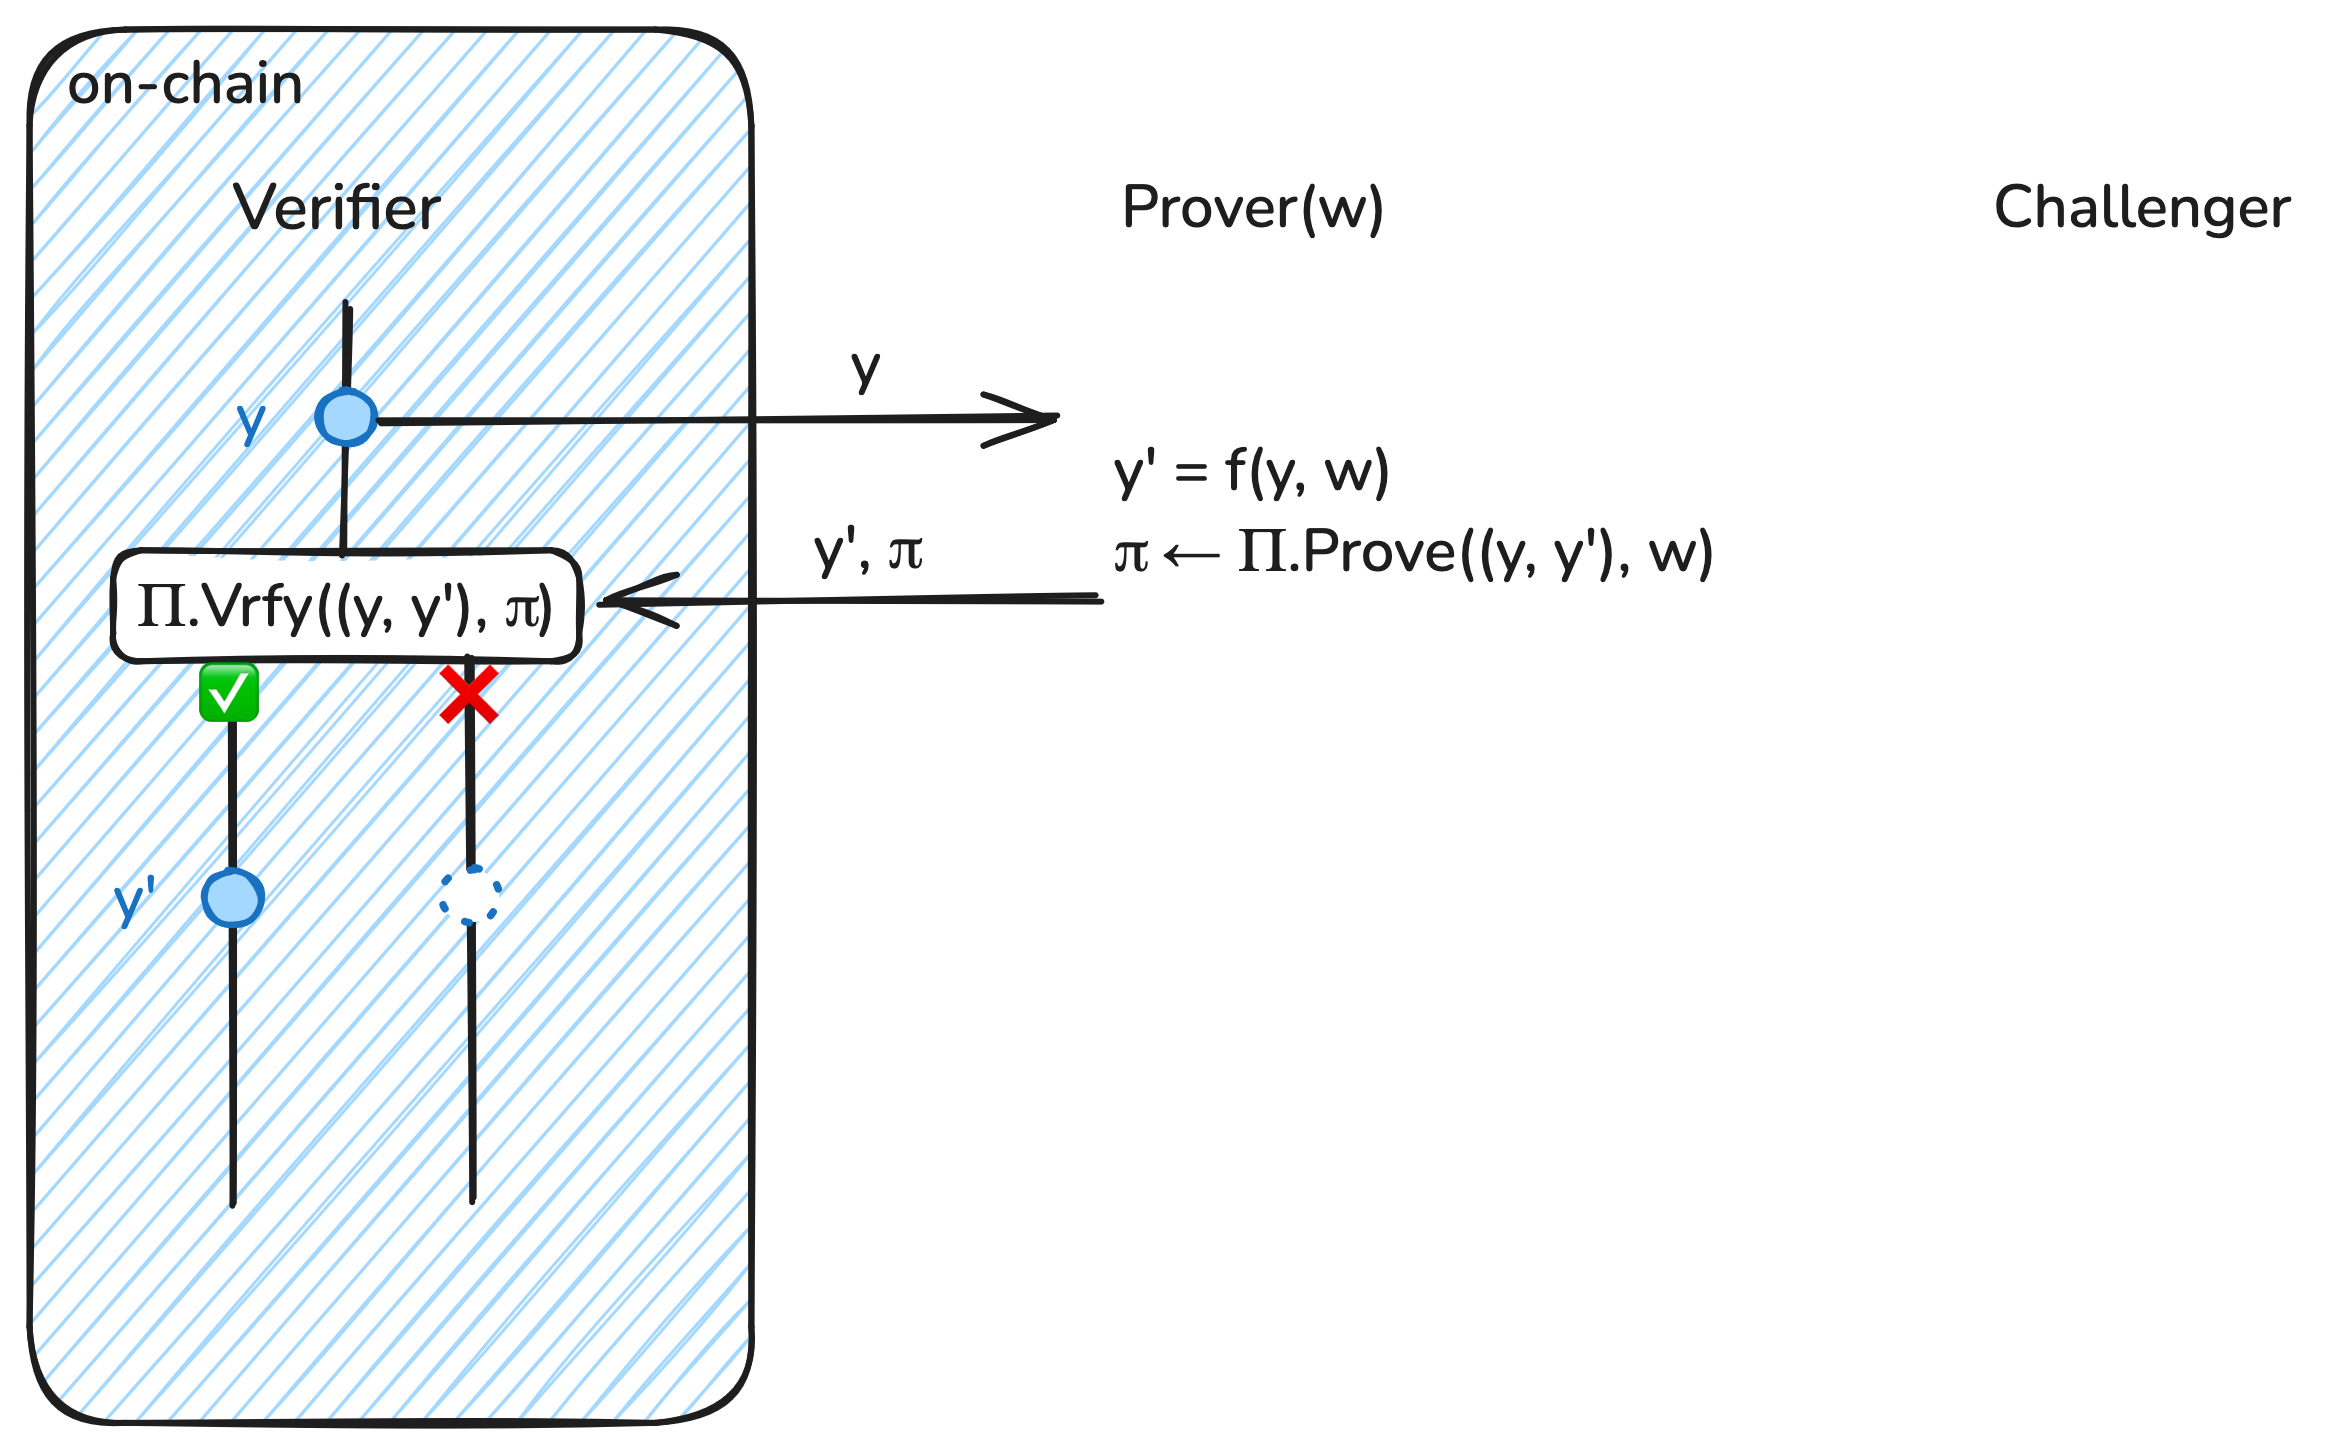
\includegraphics[width=\textwidth]{naysayer/figs/vc.png}
    \caption{\textbf{Using VC to move computation off-chain.} The off-chain ``prover'' applies the function $f$ to input $y$ and potentially an auxiliary off-chain input $w$ to get the result $y' = f(y, w)$. (In the case of a zk-rollup, $f$ is the state transition function, $y$ is the previous on-chain state, $w$ is a batch of transactions, and $y'$ is the new state after applying the transactions in $w$ to $y$.) It posts $y'$ and a proof $\pi$ of its correctness, which is verified on-chain before the output $y'$ is accepted. This paradigm does not require any challengers.\todo{update $\sf Vrfy$ to $\vrfy$ in fig}}
    \label{fig:vc}
 \end{figure}

VC leads to a paradigm in which smart contracts, while capable of arbitrary computation, primarily act as verifiers and outsource all significant computation off-chain (see \Cref{fig:vc}). A motivating application is so-called ``zk''-\emph{rollups}\footnotemark~\cite{starknet,zksync,aztec,dydx,scroll}, which combine transactions from many users into a single smart contract which verifies a proof that all have been executed correctly.
\footnotetext{The ``zk'' part of the name is often a misnomer, since these services do not necessarily offer the zero-knowledge property, and in fact most do not.} 
However, verifying these proofs can still be costly. For example, the StarkEx rollup 
%contract verifying the state transitions of the off-chain StarkEx marketplace 
has spent hundreds of thousands of dollars to date to verify FRI polynomial commitment opening proofs.\footnote{\url{https://etherscan.io/address/0x3e6118da317f7a433031f03bb71ab870d87dd2dd}}
% Even verifying simple statements can exceed the block gas limit of Ethereum~\cite{EPRINT:NRBB22}\todo{not sure about this example. Maybe a dollar figure on STARKs would more convincing?}\istvan{I had in mind the CRS for EIP-4844 that would have been exceeded the block gas limit with this solution.}.

We observe that this proof verification is often wasteful. In most applications, provers have strong incentives to post only correct proofs, suffering direct financial penalties (in the form of a lost security deposit) or indirect costs to their reputation and business for posting incorrect proofs. As a result, a significant fraction of a typical layer-1 blockchain's storage and computation is expended verifying proofs, which are almost always correct.\footnote{At the time of this writing, we are unaware of any major rollup service which has posted an incorrect proof in production.}

 \begin{figure}[tb]
    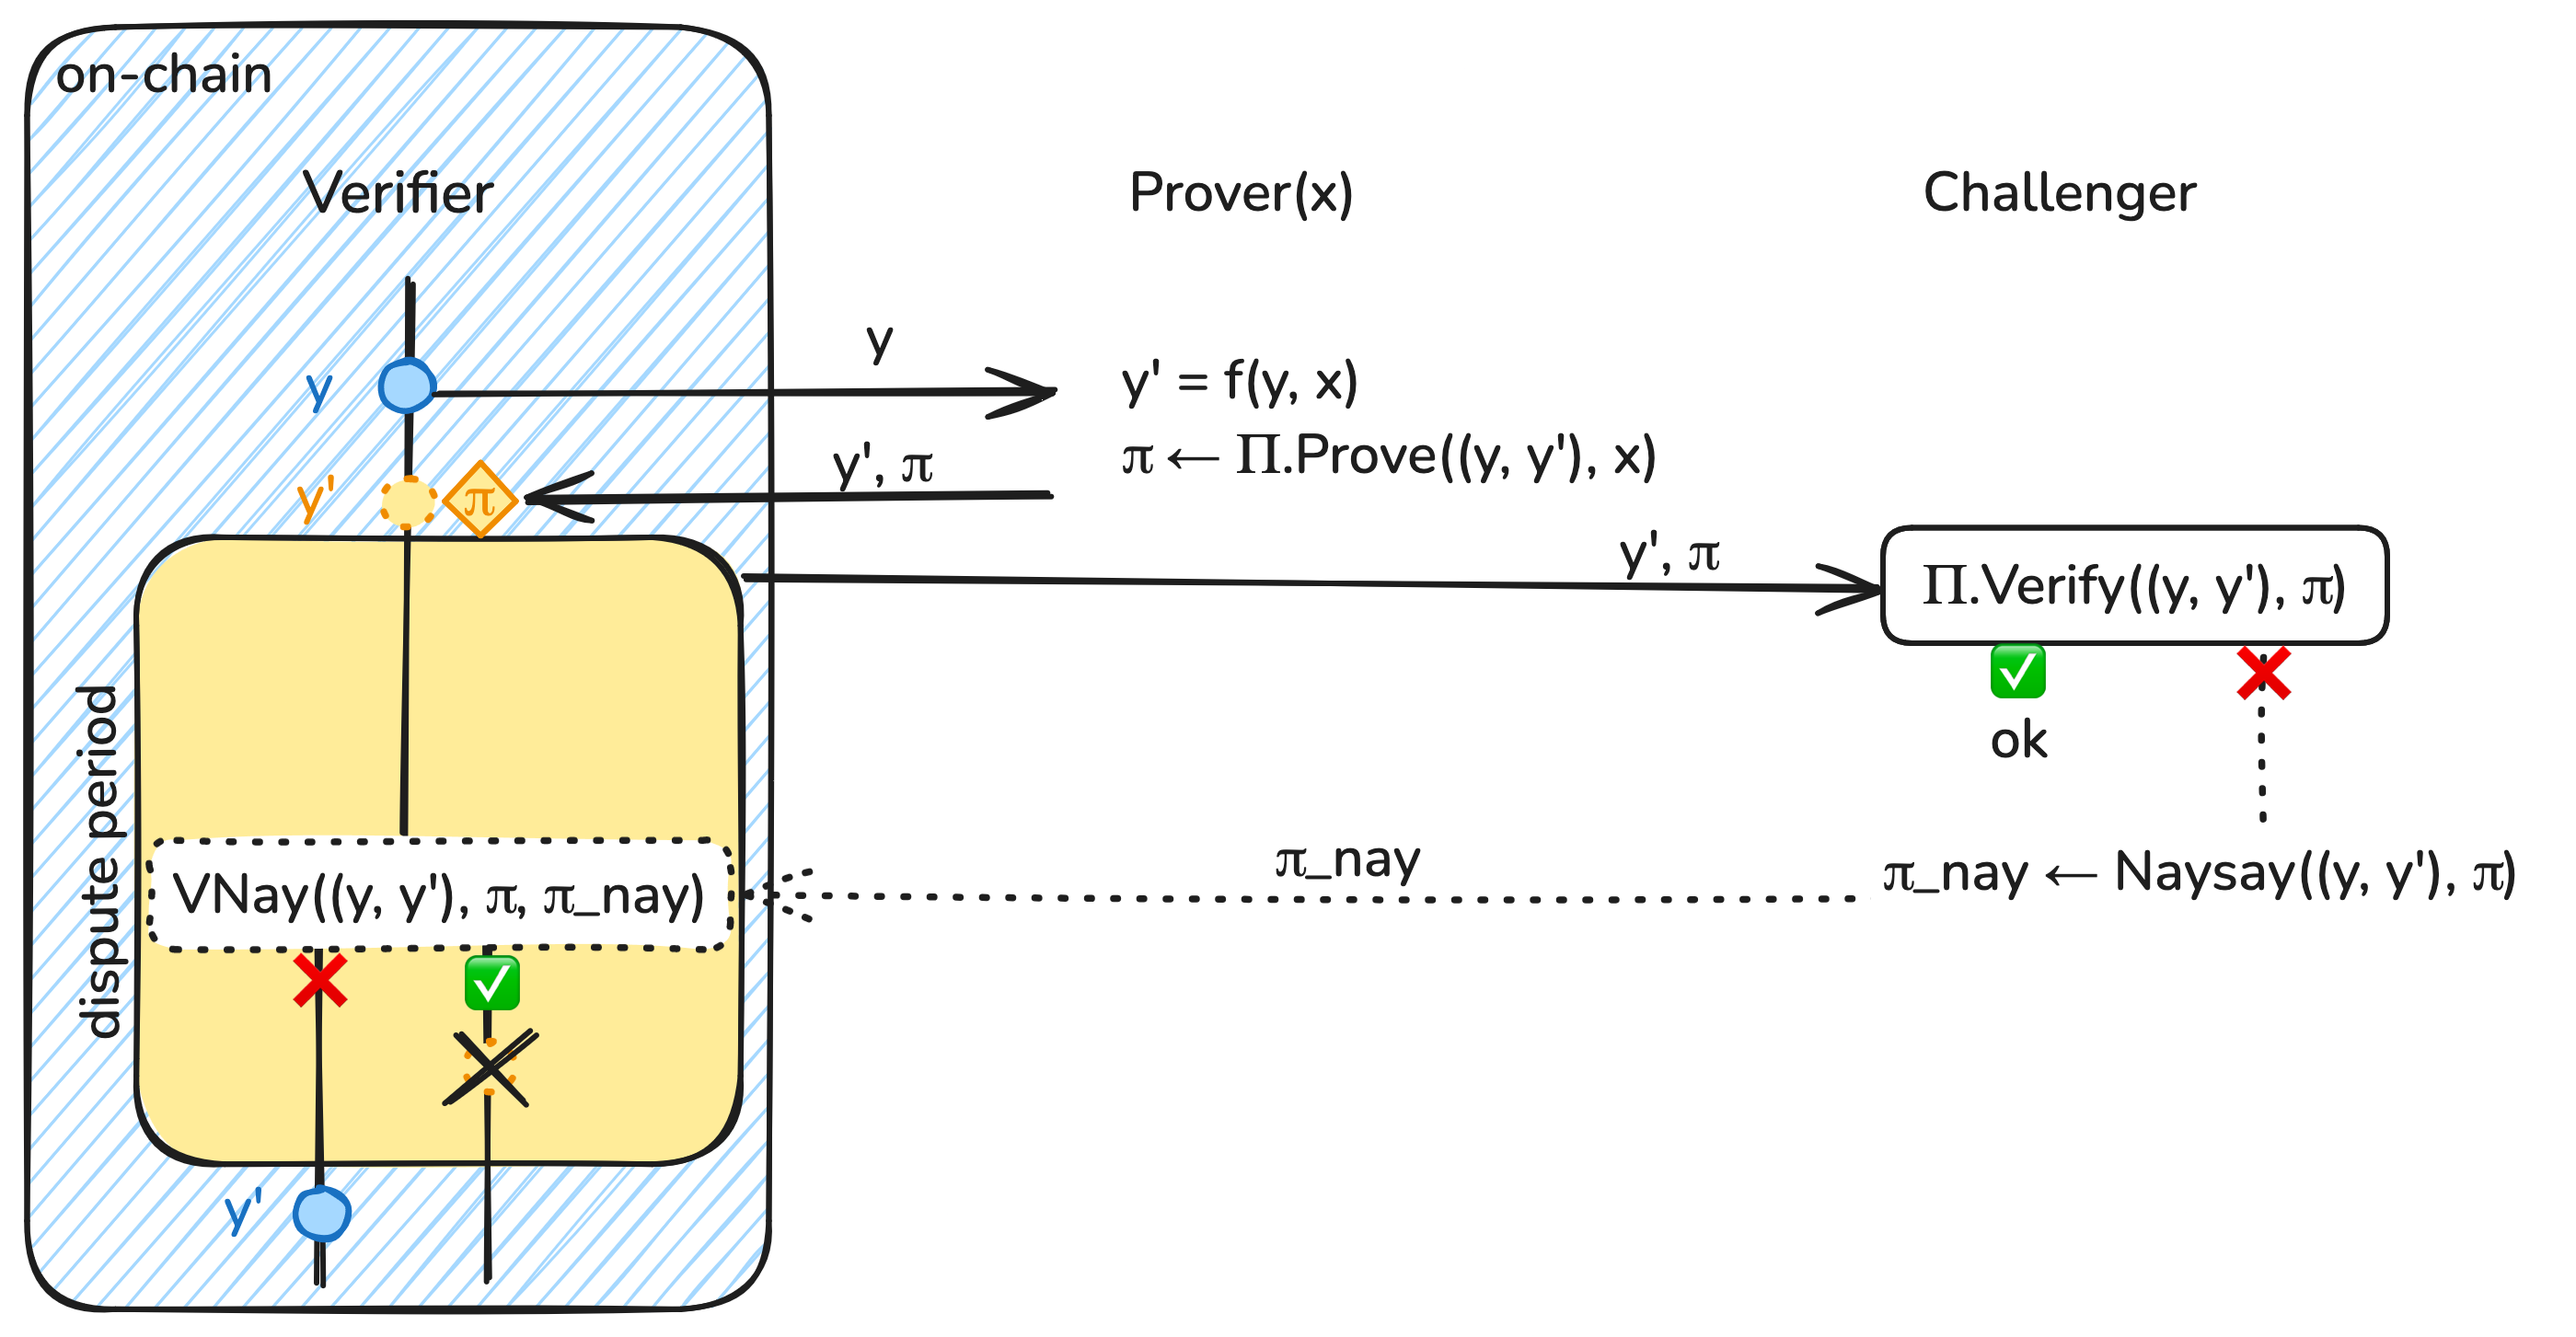
\includegraphics[width=\textwidth]{naysayer/figs/naysayer.png}
    \caption{\textbf{The naysayer proof approach.} As in VC, the off-chain prover computes $y' = f(y, w)$ and $\pi$, which it posts on-chain. This time, the proof is \emph{not} verified on-chain, but is provisionally accepted while waiting for the challenge period to pass. Any party can verify $\pi$ off-chain and, if it fails, issue a challenge by creating a naysayer proof $\pi_\nay$. The on-chain verifier checks any submitted naysayer proofs, and if they pass, it rejects the claimed result $y'$. If the challenge period elapses without any successful naysaying, $y'$ is accepted.}
    \label{fig:naysayer}
 \end{figure}

This state of affairs motivates us to propose a new paradigm called \emph{naysayer proofs} (\Cref{fig:naysayer}). In this paradigm, the verifier (e.g., a rollup smart contract) optimistically accepts a submitted proof without verifying its correctness. Instead, any observer can check the proof off-chain and, if needed, prove its \emph{incorrectness} to the verifier by submitting a \emph{naysayer proof}. The verifier then checks the naysayer proof and, if it is correct, rejects the original proof.
Otherwise, if no party successfully naysays the original proof before the end of the challenge period, the original proof is accepted.
To deter denial of service, naysayers may be required to post collateral, which is forfeited if their naysayer proof is incorrect.

This paradigm potentially saves the verifier work in two ways. 
First, in the optimistic case, where the proof is not challenged, the verifier does no work at all (just like the related fraud proof paradigm; see \Cref{sec:naysayer_related}). We expect this to almost always be the case in practice. Second, even in the pessimistic case, we will see below that checking the naysayer proof can be much more efficient than checking the original proof.
In other words, the naysayer acts as a helper to the verifier by reducing the cost of the verification procedure in fraudulent cases. At worst, checking the naysayer proof is equivalent to verifying the original proof (this is the trivial naysayer construction).

Naysayer proofs enable other interesting trade-offs. 
% for instance, %for a proof system with transparent setup and large proofs, the \naysayer proof could be instantiated generically using a short proof system with trusted setup (e.g., \cite{groth16}), or using a lower security level. 
For instance, naysayer proofs can be instantiated with a lower security level than the original proof system.
This is because a violation of the naysayer proof system's soundness undermines only the \emph{completeness} of the original proof system. %, but not its soundness. 
For an application like a rollup service, this would result in a loss of liveness; importantly, the rollup users' funds would remain secure. 
Liveness could be restored by falling back to full proof verification on-chain.

%Move this to later? Conclusion?
%The naysayer paradigm introduces a new set of criteria for evaluating the efficiency of proof systems. Previously, developers were solely focusing on the proof size and verification cost of a proof system; this paradigm allows one to instead optimize for a proof system's proof size \emph{and its accompanying naysayer proof size and verification cost}. We further detail the implications of these new selection criteria in~\Cref{sec:evaluation}.

We will formally define naysayer proofs in~\Cref{sec:naysayer_def} and show that every succinct proof system has a logarithmic-size and constant-time naysayer proof. Before that, we discuss related work in \Cref{sec:naysayer_related} and define our system model in more detail in \Cref{sec:naysayer_model}.
In~\Cref{sec:naysayer_apps}, we construct naysayer proofs for four concrete proof systems and evaluate their succinctness. % in comparison with verifying the original proof. 
We discuss storage considerations in \Cref{sec:naysayer_storage} and conclude with some open directions in~\Cref{sec:naysayer_extensions}.

\section{Preliminaries}
We use $[n]$ to denote the range $\{1, \dots, n\}$. For other ranges (mostly zero-indexed), we explicitly write the (inclusive) endpoints, e.g., $[0,n]$. 
Concatenation of vectors $\vec{x},\vec{y}$ is written as $\vec{x} || \vec{y}$. 
Let $\secpar$ be the security parameter.
We use the uppercase variable $X$ for the free variable of a polynomial, e.g., $f(X)$. 
We use a calligraphic font, e.g., $\mathcal{S}$ or $\mathcal{X}$, to denote sets or domains. When we apply an operation to two sets of equal size $\ell$ we mean pairwise application, e.g., $\mathcal{Z} = \mathcal{X} + \mathcal{Y}$ means $z_i = x_i + y_i~\forall{i \in [\ell]}$. 
Sampling an element $x$ uniformly at random from a set $\mathcal{X}$ is written as $x \sample \mathcal{X}$. 
We use $:=$ to denote variable assignment, $y \gets \mathsf{Alg}(x)$ to assign to $y$ the output of some algorithm $\mathsf{Alg}$ on input $x$, and $y \sample \mathsf{Alg}(x)$ if the algorithm is randomized. When we wish to be explicit about the randomness $r$ used, we write $y \gets \mathsf{Alg}(x; r)$. 

For a non-interactive zero-knowledge proof system $\Pi$, we write $\pi \gets \Pi.{\sf Prove}(x; w)$ to show that the proving algorithm takes as input an instance $x$ and witness $w$ and outputs a proof $\pi$. Verification is written as $\Pi.\vrfy(x, \pi)$ and outputs a bit $b$. 

We distinguish the key-pairs used in a signature scheme ($\vk, \sk$ for ``verification'' and ``signing'' key, respectively) from those used in an encryption scheme ($\ek, \dk$ for ``encryption'' and ``decryption'' key, respectively). 

\subsection{Bilinear Pairings}\label{sec:pairings}

\begin{definition}[bilinear pairing]
   A bilinear pairing is a map $e : \GG_1 \times \GG_2 \mapsto \GG_T$ where $\GG_1, \GG_2,$ and $\GG_T$ are cyclic groups of prime order $p$. (Often, $\GG_1,\GG_2$ are written in additive notation and $\GG_T$ in multiplicative notation.) Let $g_1,h_1 \in \GG_1$ and $g_2,h_2 \in \GG_2$ (generators of their respective groups). The map $e$ has the following properties:
   \begin{description}
       \item[Bilinearity:] For all $a,b \in \ZZ_p^*$, the following hold:
       \begin{align*}
           e(g_1^a, g_2) = e(g_1, g_2^a) = e(g_1, g_2)^a\\
           e(g_1 h_1, g_2) = e(g_1, g_2) \cdot e(h_1, g_2)\\
           e(g_1, g_2 h_2) = e(g_1, g_2) \cdot e(g_1, h_2)
        \end{align*}
        \item[Non-degeneracy:] $e(g_1, g_2) \neq 1$.
        \item[Computability:] There is an efficient algorithm for computing $e$.
    \end{description}
\end{definition}

Pairings are divided into types based on the (in)equality of the utilized groups $\GG_1,\GG_2$ and whether there is an efficiently computable homomorphism between the groups. For our purposes, we will use a type-3 pairing: asymmetric ($\GG_1 \neq \GG_2$) and with no such efficiently computable homomorphism. In this case, the Decisional Diffie-Hellman (DDH) assumption is believed to hold in both $\GG_1$ and $\GG_2$; this is referred to as the \emph{symmetric external Diffie-Hellman (SXDH) assumption}.

\subsection{Shamir Secret Sharing}\label{sec:shamir}
Shamir~\cite{ShamirSS} introduced a scheme to share a secret among $n$ parties such that any $t$ parties can work together to recover the secret, but with any fewer parties the secret remains information-theoretically hidden.

\begin{construction}[Shamir secret sharing \cite{ShamirSS}]
Let $p$ be a prime.
    \begin{itemize}
        \item \underline{$\{s_1, \dots, s_n\} \gets \share(s, t, n)$:} Given a secret $s \in \ZZ_p$ and $t \leq n \in \mathbb{N}$, compute a $t$-out-of-$n$ sharing of $s$ by choosing a random degree-$(t-1)$ polynomial $f(X) \in \ZZ_p[X]$ such that $f(0) = s$. For $i \in [n]$, compute $s_i := (i, f(i))$.
        \item \underline{$\{s', \perp\} \gets \recon(S, t, n)$:} Given some set of shares $S$, check if $\sizeof{S} < t$. If so, output $\perp$. Otherwise, without loss of generality, let $S' := \{s_1, \dots, s_t\}$ be the first $t$ entries of $S$, where $s_i := (x_i, y_i)$. Output the Lagrange interpolation at 0:
        \[
            s' := \sum_{i=1}^t y_i \prod_{j=1, j \neq i}^t \frac{x_j}{x_j - x_i}.
        \]
    \end{itemize}
\end{construction}

The secret sharing scheme is \emph{correct}, since for any secret $s$ and values $t \leq n \in \NN$, we have $\recon(\share(s, t, n),\allowbreak t, n) = s$. 

For notational convenience, let $\share(s,t,n; r)[i]$ denote the $i$th share of $s$ computed with randomness $r$. The reconstruction algorithm can be generalized to interpolate any point $f(k)$ (not just the secret at $k=0$) and thereby recover the $i$th share:
\begin{itemize}
    \item \underline{$\{s_k,\perp\} \gets {\sf Interpolate}(S, k, t, n)$:} If $\sizeof{S} < t$, output $\perp$. Otherwise, use the first $t$ entries $(x_1, y_1), \dots,\allowbreak (x_t, y_t)$ of $S$ to interpolate
    \[
        f(k) = \sum_{i=1}^t y_i \prod_{j=1, j \neq i}^t \frac{x_j - k}{x_j - x_i}.
    \]
    Output $s_k := (k, f(k))$.
\end{itemize}

\subsection{BLS Signatures}\label{sec:bls}

\begin{construction}[BLS signature scheme \cite{AC:BonLynSha01}]\label{con:bls}
Let $\GG_1, \GG_2$ be elliptic curve groups of order $p$ generated by $g_1$ and $g_2$, respectively, and $e: \GG_1 \times \GG_2 \rightarrow \GG_T$ be an efficiently computable asymmetric pairing between them. We also require a hash function $\blshash: \{0, 1\}^* \rightarrow \GG_1$. The signature scheme works as follows:
\begin{itemize}
\item \underline{$(\sk, \vk) \gets \kgen(\secparam)$:} Given the security parameter $1^\lambda$, sample $x \sample \ZZ_p$ and output the keypair consisting of signing key $\sk := x$ and verification key $\vk := g_2^x$.
\item \underline{$\sigma \gets \sign(\sk, m)$:} Given a signing key $\sk \in \ZZ_p$ and a message $m \in \{0,1\}^*$, compute a signature $\sigma := \blshash(m)^{sk}$.
\item \underline{$\{0,1\} \gets \vrfy(\vk, m, \sigma)$:} Given a verification key $\vk \in \GG_2$, message $m \in \bin^*$, and signature $\sigma \in \GG_1$, if $e(\sigma, g_2) = e(\blshash(m), \vk)$, output 1. Else output 0.
\end{itemize}
\end{construction}

The security of BLS relies on the gap co-Diffie Hellman assumption on $(\GG_1,\GG_2)$, i.e., co-DDH being easy but co-CDH being hard on $\GG_1,\GG_2$, as well as the existence of an efficiently computable homomorphism $\phi: \GG_2 \rightarrow \GG_1$ (type-2 pairing). Since we require a type-3 pairing for our purposes (i.e., no efficiently computable $\phi$ exists), we rely on a stronger variant of the co-GDH assumption (see discussion in \cite[\S3.1]{AC:BonLynSha01} and \cite[\S2.2]{EPRINT:SmaVer05}).

\paragraph{Threshold variant}
Sharing a BLS signing key $\sk \in \ZZ_p$ via Shamir secret sharing leads directly to a robust $t$-out-of-$n$ threshold signature \cite{AC:BonLynSha01}.
More specifically, each party $i \in [n]$ receives a $t$-out-of-$n$ Shamir secret share $\sk_i$ of the key. The ``partial'' public keys $\vk_i := g_2^{\sk_i}$ are published along with the public key $\vk$.

A partial signature is computed in exactly the same way as a regular BLS signature, but under the secret key share: $\sigma_i := \blshash(m)^{\sk_i}$. This value is publicly verifiable by checking that $(g_2, \vk_i, \blshash(m), \sigma_i)$ is a co-Diffie-Hellman tuple (i.e., it is of the form $(g_2, g_2^a, h, h^a)$ where $g_2 \in \GG_2$ and $h \in \GG_1$).

 Given $t$ valid partial signatures on a message $m \in \{0,1\}^*$ anyone can recover a regular BLS signature:

\begin{itemize}
    \item \underline{$\sigma \gets \recon(S := \{(i, \sigma_i)\})$}: Let $S' \subseteq S$ be the set of valid partial signatures in $S$. If $\sizeof{S'} < t$, output $\perp$. Otherwise, without loss of generality, assume the first $t$ valid signatures come from users $1, \dots, t$ and recover the complete signature as
    \[
        \sigma \gets \prod_{i=1}^t \sigma_i^{\lambda_i}, \text{ where } \lambda_i = \prod_{j=1,j\neq i}^t \frac{j}{j-i} \pmod{p}
    \]
\end{itemize}

Notice that the reconstruction simply performs Shamir reconstruction of the signing key shares $\sk_i$ in the exponent and thus the output will equal $\blshash(m)^{\sk}$. Hence, the complete signature is indistinguishable from a regular BLS signature, and verification proceeds exactly as in the regular scheme.

\subsection{KZG polynomial commitments}\label{sec:kzg}

We give the asymmetric version of KZG below.

\begin{construction}[KZG polynomial commitments~\cite{AC:KatZavGol10}]
Let $\GG_1, \GG_2$ be elliptic curve groups of order $p$ with generators $g_1,g_2$ and $e: \GG_1 \times \GG_2 \mapsto \GG_T$ be an elliptic curve pairing. The following is a commitment scheme for polynomials in $\ZZ_p[X]$ with degree at most $d$.
\begin{itemize}
    \item \underline{$\crs \gets \setup(d):$} Sample $\tau \sample \ZZ_p$ and output $\crs := \{g_1, g_1^\tau, g_1^{\tau^2}, \dots, g_1^{\tau^d}, g_2, g_2^\tau\}$.
    \item \underline{$\com_f \gets \Commit(\crs, f(X)):$} Let $f(X) = a_0 + a_1 X + \dots + a_d X^d \in \ZZ_p[X]$. Use $\crs$ to compute and output $g_1^{f(\tau)} = g_1^{a_0} \cdot (g_1^\tau)^{a_1} \dots (g_1^{\tau^d})^{a_d} = g_1^{a_0 + a_1 \tau + \dots + a_d \tau^d} \in \GG_1$.
    \item \underline{$(f(i), \pi_i) \gets \Open(\crs, f(X), i):$} To open $f(X)$ at $i$, let $q_i(X) := \frac{f(X) - f(i)}{X - i} \in \ZZ_p[X]$\footnote{This is a polynomial by Little Bézout's Theorem.}. Then compute $\com_{q_i} \gets \Commit(\crs, q_i(X))$ and output $(f(i), \com_{q_i}) \in \ZZ_p \times \GG_1$.
    \item \underline{$\{0,1\} \gets \vrfy(\crs, \com_f, i, y, \pi_i):$} To confirm $y = f(i)$, it suffices to check that $q_i(X) = \frac{f(X) - y}{X - i}$ at $X=\tau$. This can be done with a single pairing check:
    \[
        e(\com_f / g_1^y, g_2) \stackrel{?}{=} e(\pi_i, g_2^\tau / g_2^i)
    \]
\end{itemize}
\end{construction}

% Notice that this scheme is linearly homomorphic: given commitments $\com_f, \com_{f'}$ to two distinct polynomials $f(X),f'(X)$, the commitment to $(f+f')(X)$ is $\com_{f+f'} := \com_f \cdot \com_{f'}$. The same holds with the corresponding evaluation proofs $\pi_{f,i}, \pi_{f',i}$ at some point $i$: the evaluation proof for the point $(f+f')(i)$ is $\pi_{f+f',i} := \pi_{f,i} \cdot \pi_{f',i}$. Scaling the polynomial $f(X)$ by a constant $c \in \ZZ_p$ is also simple: the new commitment is $\com_{cf} := \com_f^c$ and an adjusted evaluation proof is obtained as $\pi_{cf, i} := \pi_{f,i}^c$.

The security of the scheme relies on the $d$-Strong Diffie Hellman assumption ($d$-SDH), which states that given $\{g_1, g_1^\tau, \dots, g_1^{\tau^d}, g_2, g_2^\tau\}$, it is difficult to compute $(c, g_1^{\frac{1}{\tau-c}})$ for any $c \in \ZZ_p \setminus \{-\tau\}$. This assumption is stronger than $d$-SDH in $\GG_1$, which in turn implies DDH in $\GG_1$.

\subsection{Pedersen Commitments}\label{sec:pedersen}

Next, we recall Pedersen commitments~\cite{C:Pedersen91}, a commitment scheme which is unconditionally (information-theroetically) hiding and computationally binding (by the discrete logarithm assumption on $\GG$). In our construction we will instantiate the scheme over $\GG_1$, so we let $\GG = \GG_1$ in the description below.

\begin{construction}[Pedersen commitment scheme~\cite{C:Pedersen91}]
Let $\GG_1$ be a group of order $p$ and $g_1,h_1$ be generators of $\GG_1$. The following is a commitment scheme for elements $x \in \ZZ_p$.
\begin{itemize}
    \item \underline{$(\com, \decom) \gets \Commit(x):$} Sample $r \sample \ZZ_p$ and return $\com := g_1^x h_1^r$ and decommitment information $(x, r)$.
    \item \underline{$(x, r) \gets \Open(\com, \decom):$} To open $\com$, directly output $\decom = (x, r)$.
    \item \underline{$\{0,1\} \gets \vrfy(\com, x, r):$} To confirm the opening of $\com$ to $x$, it suffices to check that $\com = g_1^x h_1^r$.
\end{itemize}
\end{construction}

A PoK of the committed value can be computed using a Sigma protocol due to Okamoto~\cite{C:Okamoto92}, which can be made non-interactive using the Fiat-Shamir transform~\cite{C:FiaSha86}. We refer to this protocol as $\Pi_{\sf ped}$ and present it in \Cref{fig:pi_ped}.

\begin{figure*}[tbh]
   \centering
   \begin{mdframed}
   \begin{center}
       \textsc{PoK of Pedersen opening ($\Pi_{\sf ped}$)}
   \end{center}
   \medskip
   \textbf{Parameters:} Group $\GG_1$ of order $p$ with generators $g_1, h_1$.
   \hfill\medskip\\
   \underline{$\mathsf{Prove}(\com_{\sf ped}; (v, r)) \to \pi_{\sf ped}$:} Given a Pedersen commitment $\com_{\sf ped} = g_1^v h_1^r$, a party can prove knowledge of the opening $(v,r)$ as follows:
   \begin{enumerate}
       \item The prover samples $s_1, s_2 \sample \ZZ_p$ and sends $a := g_1^{s_1} h_1^{s_2}$ to the verifier.
       \item The verifier sends back a uniform challenge $c \sample \ZZ_p$.
       \item The prover computes $t_1 := s_1 + vc$ and $t_2 := s_2 + rc$ and sends both values to the verifier.
   \end{enumerate}
   The proof is defined as $\pi_{\sf ped} := (a, c, (t_1, t_2))$.\medskip\\
   \underline{$\vrfy(\com_{\sf ped}, \pi_{\sf ped}) \to \{0,1\}$:} Given the commitment $\com_{\sf ped}$ and a proof $\pi_{\sf ped}$, the verifier parses $\pi_{\sf ped} := (a, c, (t_1, t_2))$ and outputs 1 iff $a \cdot \com_{\sf ped}^c = g_1^{t_1} h_1^{t_2}$.
   \end{mdframed}
   \caption{The proof system $\Pi_{\sf ped}$ used to prove knowledge of the opening to a Pedersen commitment~\cite{C:Okamoto92}.}
   \label{fig:pi_ped}
\end{figure*}

\subsection{Leftover Hash Lemma}\label{sec:lhl}  

We use the presentation of the leftover hash lemma (LHL)~\cite{FOCS:ImpZuc89} from~\cite{EC:AMPR19}.\footnote{We specifically use the improved version from the Journal of Cryptology version of this paper.}  Let $\left(\mathcal{X},\oplus\right)$ be a finite group of size $\left|\mathcal{X}\right|$, and let $n$ be a positive integer. For any fixed $2n$-vector of group elements $\mathbf{x} = \left\lbrace x_{j,b} \right\rbrace_{j\in \left[ n \right],b\in\left\lbrace 0,1 \right\rbrace} \in\mathcal{X}^{2n}$, denote by $\mathcal{S}_{\mathbf{x}}$ the following distribution:
\begin{equation}
	\mathcal{S}_{\mathbf{x}} = \Big\{\bigoplus_{j\in[n]}x_{j,r_j} : \left(r_1,\cdots,r_n\right)\gets\left\lbrace 0,1 \right\rbrace^n\Big\}.\nonumber
\end{equation}
Also, let $\mathcal{U}_{\mathcal{X}}$ denote the uniform distribution over $\mathcal{X}$, and let $\Delta \left(\mathcal{D}_1,\mathcal{D}_2\right)$ denote the statistical distance between the distributions $\mathcal{D}_1$ and $\mathcal{D}_2$. We will use the following special case of leftover hash lemma~\cite{FOCS:ImpZuc89}. The proof can be found in the JoC version of~\cite{EC:AMPR19}.

\begin{lemma}{\textnormal{(Leftover Hash Lemma.)}}
	\label{lemma:LHL}	
	Let $\left(\mathcal{X},\oplus\right)$ be a finite group, and let $\mathcal{S}_{\mathbf{x}}$ and $\mathcal{U}_{\mathcal{X}}$ be two distributions over $\mathcal{X}$ as defined above. For any (large enough) positive integer $n$, it holds that
	\begin{equation}
		\Pr_{\mathbf{x}\gets\mathcal{X}^{2n}}\left[\Delta\left(\mathcal{S}_{\mathbf{x}},\mathcal{U}_{\mathcal{X}}\right)> \sqrt[4]{\frac{\sizeof{\mathcal{X}}}{2^n}}  \right]\leq \sqrt[4]{\frac{\sizeof{\mathcal{X}}}{2^n}} \nonumber.
	\end{equation}
	In particular, for any $n > \log(\sizeof{\mathcal{X}}) + \omega(\log(\lambda))$, if $\mathbf{x}$ is sampled uniformly then with overwhelming probability the statistical distance between two distributions is negligible.
\end{lemma}

\subsection{Universal Composability (UC) Framework}\label{sec:uc}

In the universal composability (UC) framework~\cite{FOCS:Canetti01}, the security requirements of a protocol are defined via an \emph{ideal functionality} which is executed by a trusted party. To prove that a protocol \emph{UC-realizes} a given ideal functionality, we show that the execution of this protocol (in the real or hybrid world) can be \emph{emulated} in the ideal world, where in both worlds there is an additional adversary $\env$ (the environment) which models arbitrary concurrent protocol executions. Specifically, we show that for any adversary $\adv$ attacking the protocol execution in the real world (by controlling communication channels and corrupting parties involved in the protocol execution), there exists an adversary $\Sim$ (the simulator) in the ideal world who can produce a protocol execution which no environment $\env$ can distinguish from the real-world execution.

Below we describe the UC framework as it is presented in \cite{EPRINT:CLOS02}. 
All parties are represented as probabilistic interactive Turing machines (ITMs) with input, output, and ingoing/outgoing communication tapes. For simplicity, we assume that all communication is authenticated, so an adversary can only delay but not forge or modify messages from parties involved in the protocol. Therefore, the order of message delivery is also not guaranteed (asynchronous communication). We consider a PPT malicious, adaptive adversary who can corrupt or tamper with parties at any point during the protocol execution.
%(modeled in the ideal world via the interfaces in \Cref{fig:FSign3}).

The execution in both worlds consists of a series of sequential party activations. Only one party can be activated at a time (by writing a message on its input tape). In the real world, the execution of a protocol $\Pi$ occurs among parties $P_1, \dots, P_n$ with adversary $\adv$ and environment $\env$. In the ideal world, interaction takes place between dummy parties $\tilde{P}_1, \dots, \tilde{P}_n$ communicating with the ideal functionality $\F$, with the adversary (simulator) $\Sim$ and environment $\env$. Every copy of $\F$ is identified by a unique session identifier $\texttt{sid}$. 
% The environment $\env$ can read all parties' output tapes and write to any party's input tape, including the adversary $\adv$ or $\Sim$. $\adv$ can read the outgoing communication tapes of all parties $P_i$ and \emph{deliver} messages between parties by writing them on the corresponding incoming communication tape (this models the asynchronous but authenticated communication). $\adv$ can also \emph{corrupt} any party $P_i$, and $\env$ will be notified. In the ideal world, the dummy parties simply copy any input they receive to their outgoing communication tape. $\Sim$ interacts primarily with the ideal functionality $\F$ in several ways: it can \emph{read} the public headers of any messages on its incoming and and outgoing communication tapes, \emph{write} on $\F$'s incoming communication tape, or \emph{deliver} messages from $\F$ to a dummy party or vice versa. It can also \emph{corrupt} any dummy party $\tilde{P}_i$, and $\env$ and $\F$ will be notified.

In both the real and ideal worlds, the environment is activated first and activates either the adversary ($\adv$ resp. $\Sim$) or an uncorrupted (dummy) party by writing on its input tape. If $\adv$ (resp. $\Sim$) is activated, it can take an action or return control to $\env$. After a (dummy) party (or $\F$) is activated, control returns to $\env$. The protocol execution ends when $\env$ completes an activation without writing on the input tape of another party.

We denote with $\real_{\Pi,\adv,\env}(\secpar,x)$ the random variable describing the output of the real-world execution of $\Pi$ with security parameter $\secpar$ and input $x$ in the presence of adversary $\adv$ and environment $\env$. We write the corresponding distribution ensemble as $\{ \real_{\Pi,\adv,\env}(\secpar, x) \}_{\secpar \in \mathbb{N}, x \in \{0,1\}^*}$. The output of the ideal-world interaction with ideal functionality $\F$, adversary (simulator) $\Sim$, and environment $\env$ is represented by the random variable $\ideal_{\F,\Sim,\env}(\secpar, x)$ and corresponding distribution ensemble $\{ \ideal_{\F,\Sim,\env}(\secpar, x) \}_{\secpar \in \mathbb{N}, x \in \{0,1\}^*}$.

The actions each party can take are summarized below:
\begin{itemize}
   \item Environment $\env$: \textbf{read} output tapes of the adversary ($\adv$ or $\Sim$) and any uncorrupted (dummy) parties; then \textbf{write} on the input tape of one party (the adversary $\adv$ or $\Sim$ or any uncorrupted (dummy) parties).
   \item Adversary $\adv$: \textbf{read} its own tapes and the outgoing communication tapes of all parties; then \textbf{deliver} a pending message to party by writing it on the recipient's ingoing communication tape \emph{or} \textbf{corrupt} a party (which becomes inactive: its tapes are given to $\adv$ and $\adv$ controls its actions from this point on, and $\env$ is notified of the corruption).
   \item Real-world party $P_i$: only follows its code (potentially writing to its output tape or sending messages via its outgoing communication tape).
   \item Dummy party $\tilde{P}_i$: acts only as a simple relay with the ideal functionality $\F$, copying inputs from its input tape to its outgoing communication tape (to $\F$) and any messages received on its ingoing communication tape (from $\F$) to its output tape.
   \item Adversary $\Sim$: \textbf{read} its own input tape and the public headers (see below) of the messages on $\F$'s and dummy parties' outgoing communication tapes; then \textbf{deliver} a message to $\F$ from a dummy party or vice versa by copying it from the sender's outgoing communication tape to the recipient's incoming communication tape \emph{or} \textbf{send} its own message to $\F$ by writing on the latter's incoming communication tape \emph{or} \textbf{corrupt} a dummy party (which becomes inactive: its tapes are given to $\Sim$ and $\Sim$ controls its actions from this point on, and $\env$ and $\F$ are notified of the corruption).
   \item Ideal functionality $\F$: \textbf{read} incoming communication tape; then \textbf{send} any messages specified by its definition to the dummy parties and/or adversary $\Sim$ by writing to its outgoing communication tape.
\end{itemize}

\begin{definition}
    We say a protocol $\Pi$ \emph{UC-realizes} an ideal functionality $\F$ if for any PPT adversary $\adv$, there exists a simulator $\Sim$ such that for any environment $\env$, the distribution ensembles $\{ \real_{\Pi,\adv,\env}(\secpar, x) \}_{\secpar \in \mathbb{N}, x \in \bin^*}$ and $\{ \ideal_{\F,\Sim,\env}(\secpar, x) \}_{\secpar \in \mathbb{N},x \in \bin^*}$ are computationally indistinguishable.
\end{definition}

\section{Naysayer Proofs}\label{sec:naysayer}
\textit{(Parts of this section are taken/adapted from \cite{FC:SerGlaBon24}.)}

\bigskip
In most blockchains with programming capabilities, e.g., Ethereum~\cite{ethereum_yellowpaper}, developers are incentivized to minimize the storage and computation complexity of on-chain programs. Applications with high compute or storage incur significant fees, commonly referred to as \emph{gas}, to compensate validators in the network. Often, these costs are passed on to users of an application. 

High gas costs have motivated many applications to utilize \emph{verifiable computation (VC)}~\cite{C:GenGenPar10}, off-loading expensive operations to powerful but untrusted off-chain entities who perform arbitrary computation and provide a short proof\footnote{More precisely, a succinct non-interactive argument of knowledge, or SNARK.} that the claimed result is correct.
This computation can even depend on secret inputs not known to the verifier by relying on zero-knowledge proofs (i.e., zkSNARKs).
 %In some cases (though not all), this proof is also zero-knowledge, hiding some inputs to the computation. This is commonly referred to as a \emph{zk-rollup} (even if it is not zero-knowledge).

 \begin{figure}[tbh]
    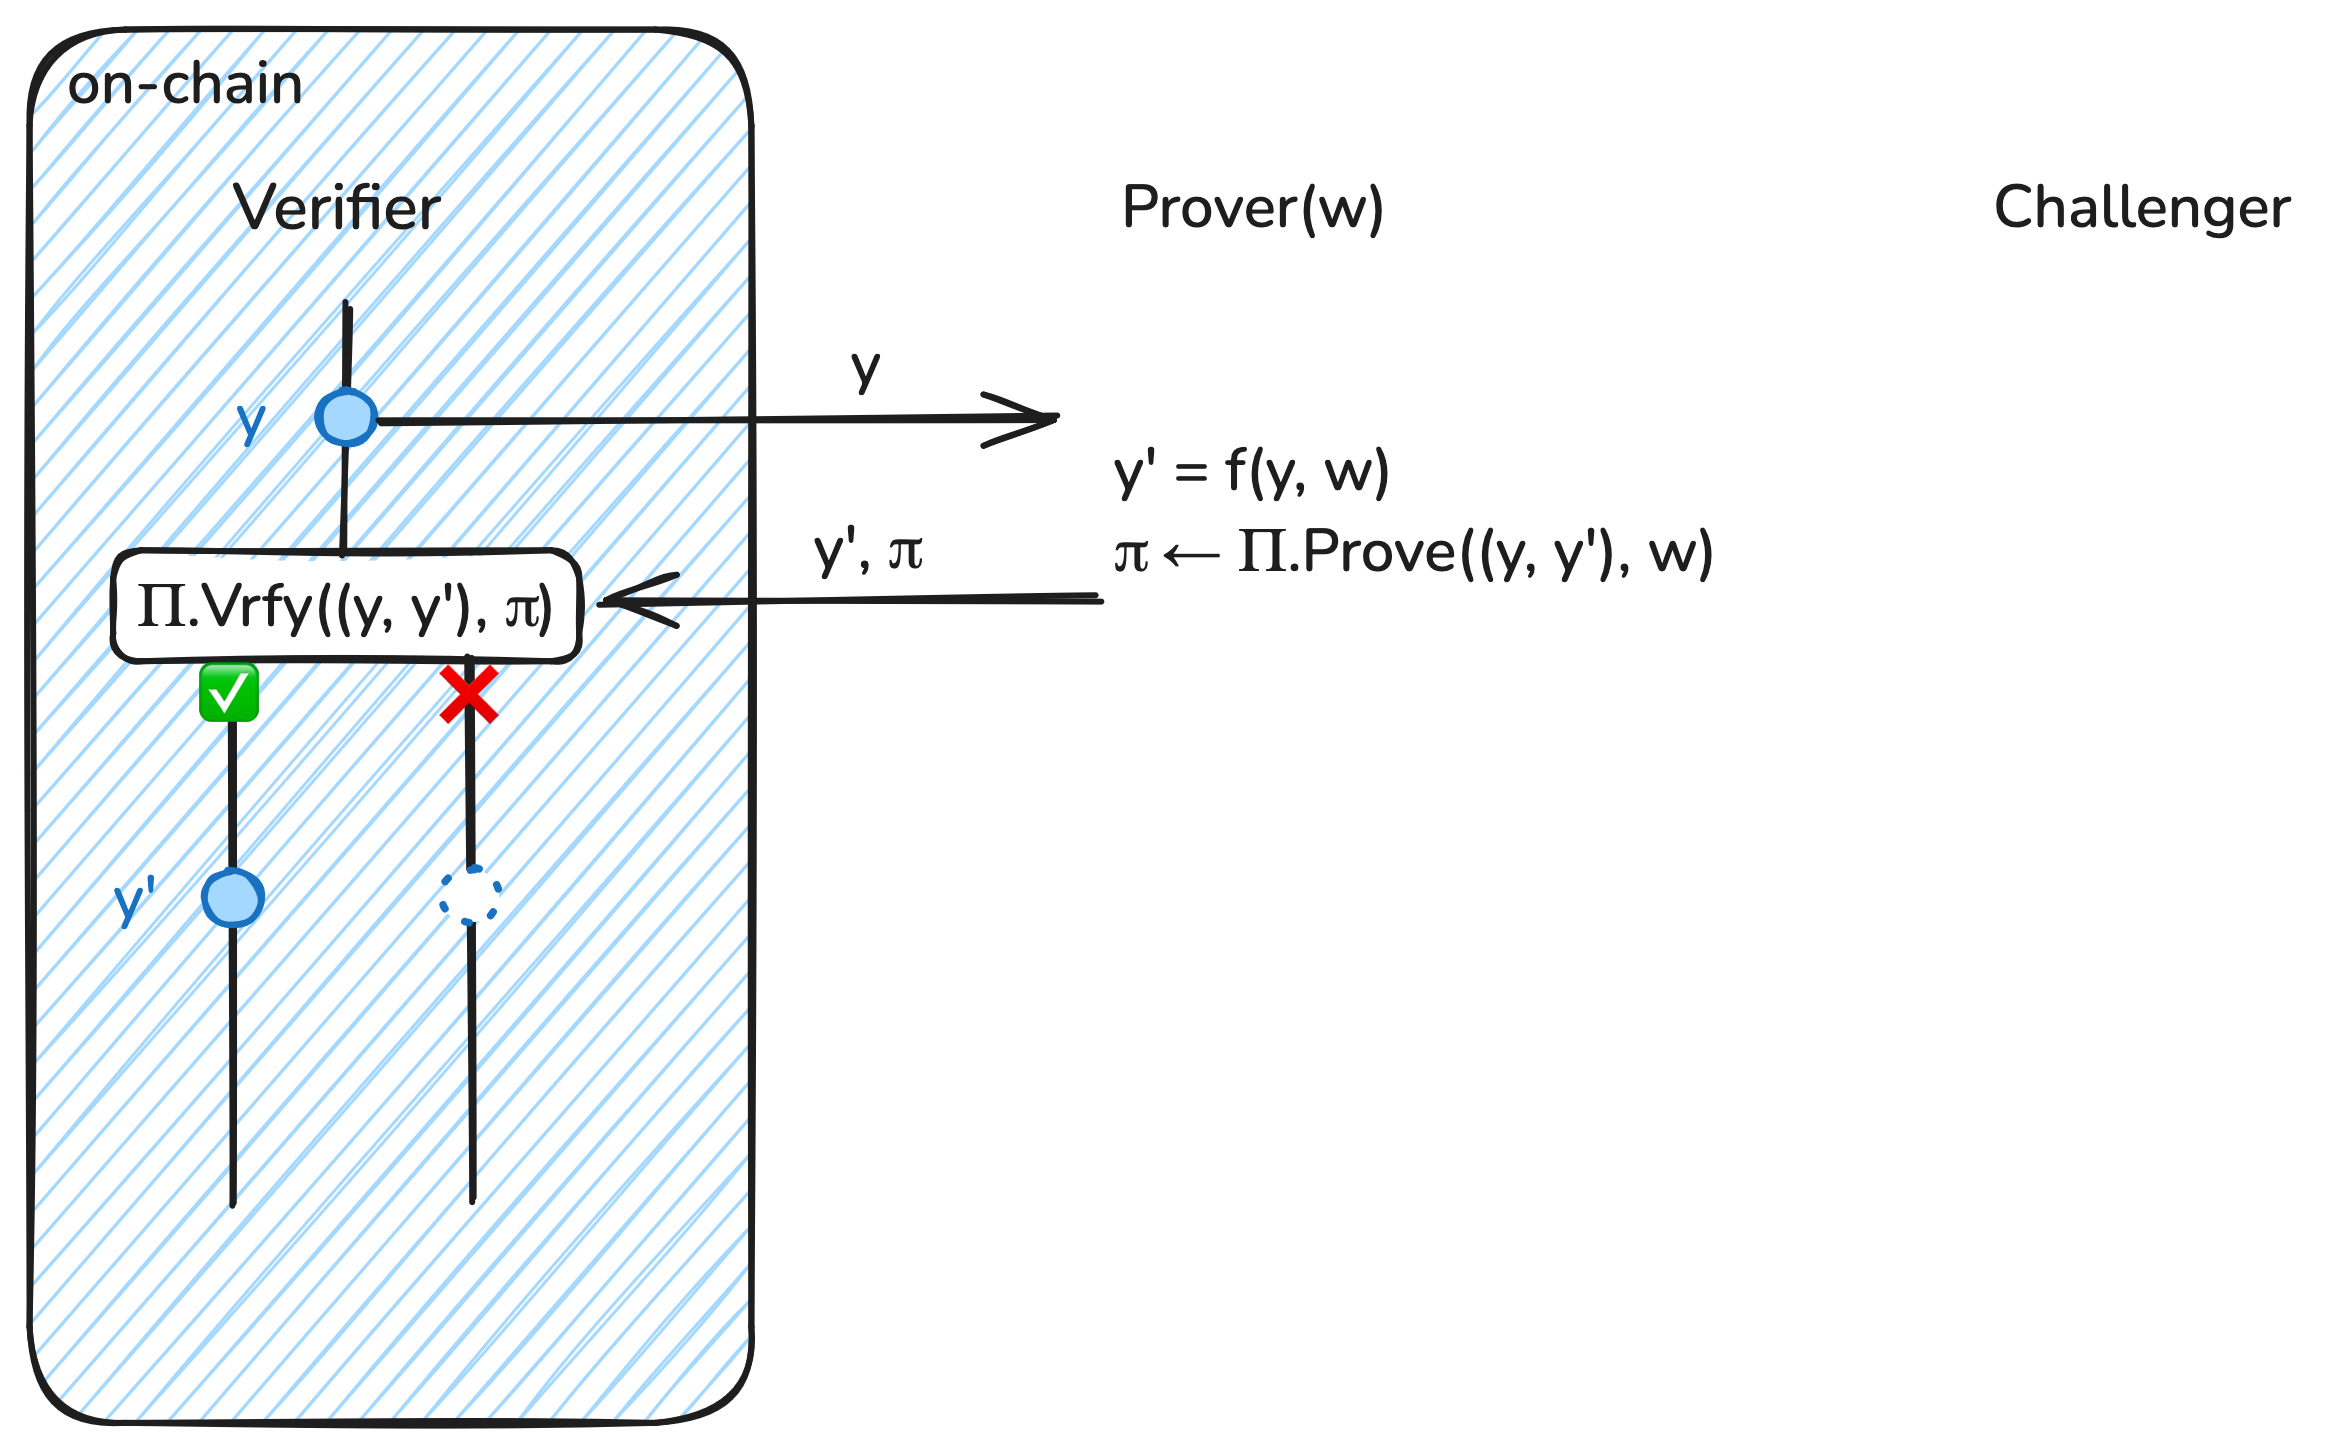
\includegraphics[width=\textwidth]{naysayer/figs/vc.png}
    \caption{\textbf{Using VC to move computation off-chain.} The off-chain ``prover'' applies the function $f$ to input $y$ and potentially an auxiliary off-chain input $w$ to get the result $y' = f(y, w)$. (In the case of a zk-rollup, $f$ is the state transition function, $y$ is the previous on-chain state, $w$ is a batch of transactions, and $y'$ is the new state after applying the transactions in $w$ to $y$.) It posts $y'$ and a proof $\pi$ of its correctness, which is verified on-chain before the output $y'$ is accepted. This paradigm does not require any challengers.\todo{update $\sf Vrfy$ to $\vrfy$ in fig}}
    \label{fig:vc}
 \end{figure}

VC leads to a paradigm in which smart contracts, while capable of arbitrary computation, primarily act as verifiers and outsource all significant computation off-chain (see \Cref{fig:vc}). A motivating application is so-called ``zk''-\emph{rollups}\footnotemark~\cite{starknet,zksync,aztec,dydx,scroll}, which combine transactions from many users into a single smart contract which verifies a proof that all have been executed correctly.
\footnotetext{The ``zk'' part of the name is often a misnomer, since these services do not necessarily offer the zero-knowledge property, and in fact most do not.} 
However, verifying these proofs can still be costly. For example, the StarkEx rollup 
%contract verifying the state transitions of the off-chain StarkEx marketplace 
has spent hundreds of thousands of dollars to date to verify FRI polynomial commitment opening proofs.\footnote{\url{https://etherscan.io/address/0x3e6118da317f7a433031f03bb71ab870d87dd2dd}}
% Even verifying simple statements can exceed the block gas limit of Ethereum~\cite{EPRINT:NRBB22}\todo{not sure about this example. Maybe a dollar figure on STARKs would more convincing?}\istvan{I had in mind the CRS for EIP-4844 that would have been exceeded the block gas limit with this solution.}.

We observe that this proof verification is often wasteful. In most applications, provers have strong incentives to post only correct proofs, suffering direct financial penalties (in the form of a lost security deposit) or indirect costs to their reputation and business for posting incorrect proofs. As a result, a significant fraction of a typical layer-1 blockchain's storage and computation is expended verifying proofs, which are almost always correct.\footnote{At the time of this writing, we are unaware of any major rollup service which has posted an incorrect proof in production.}

 \begin{figure}[tb]
    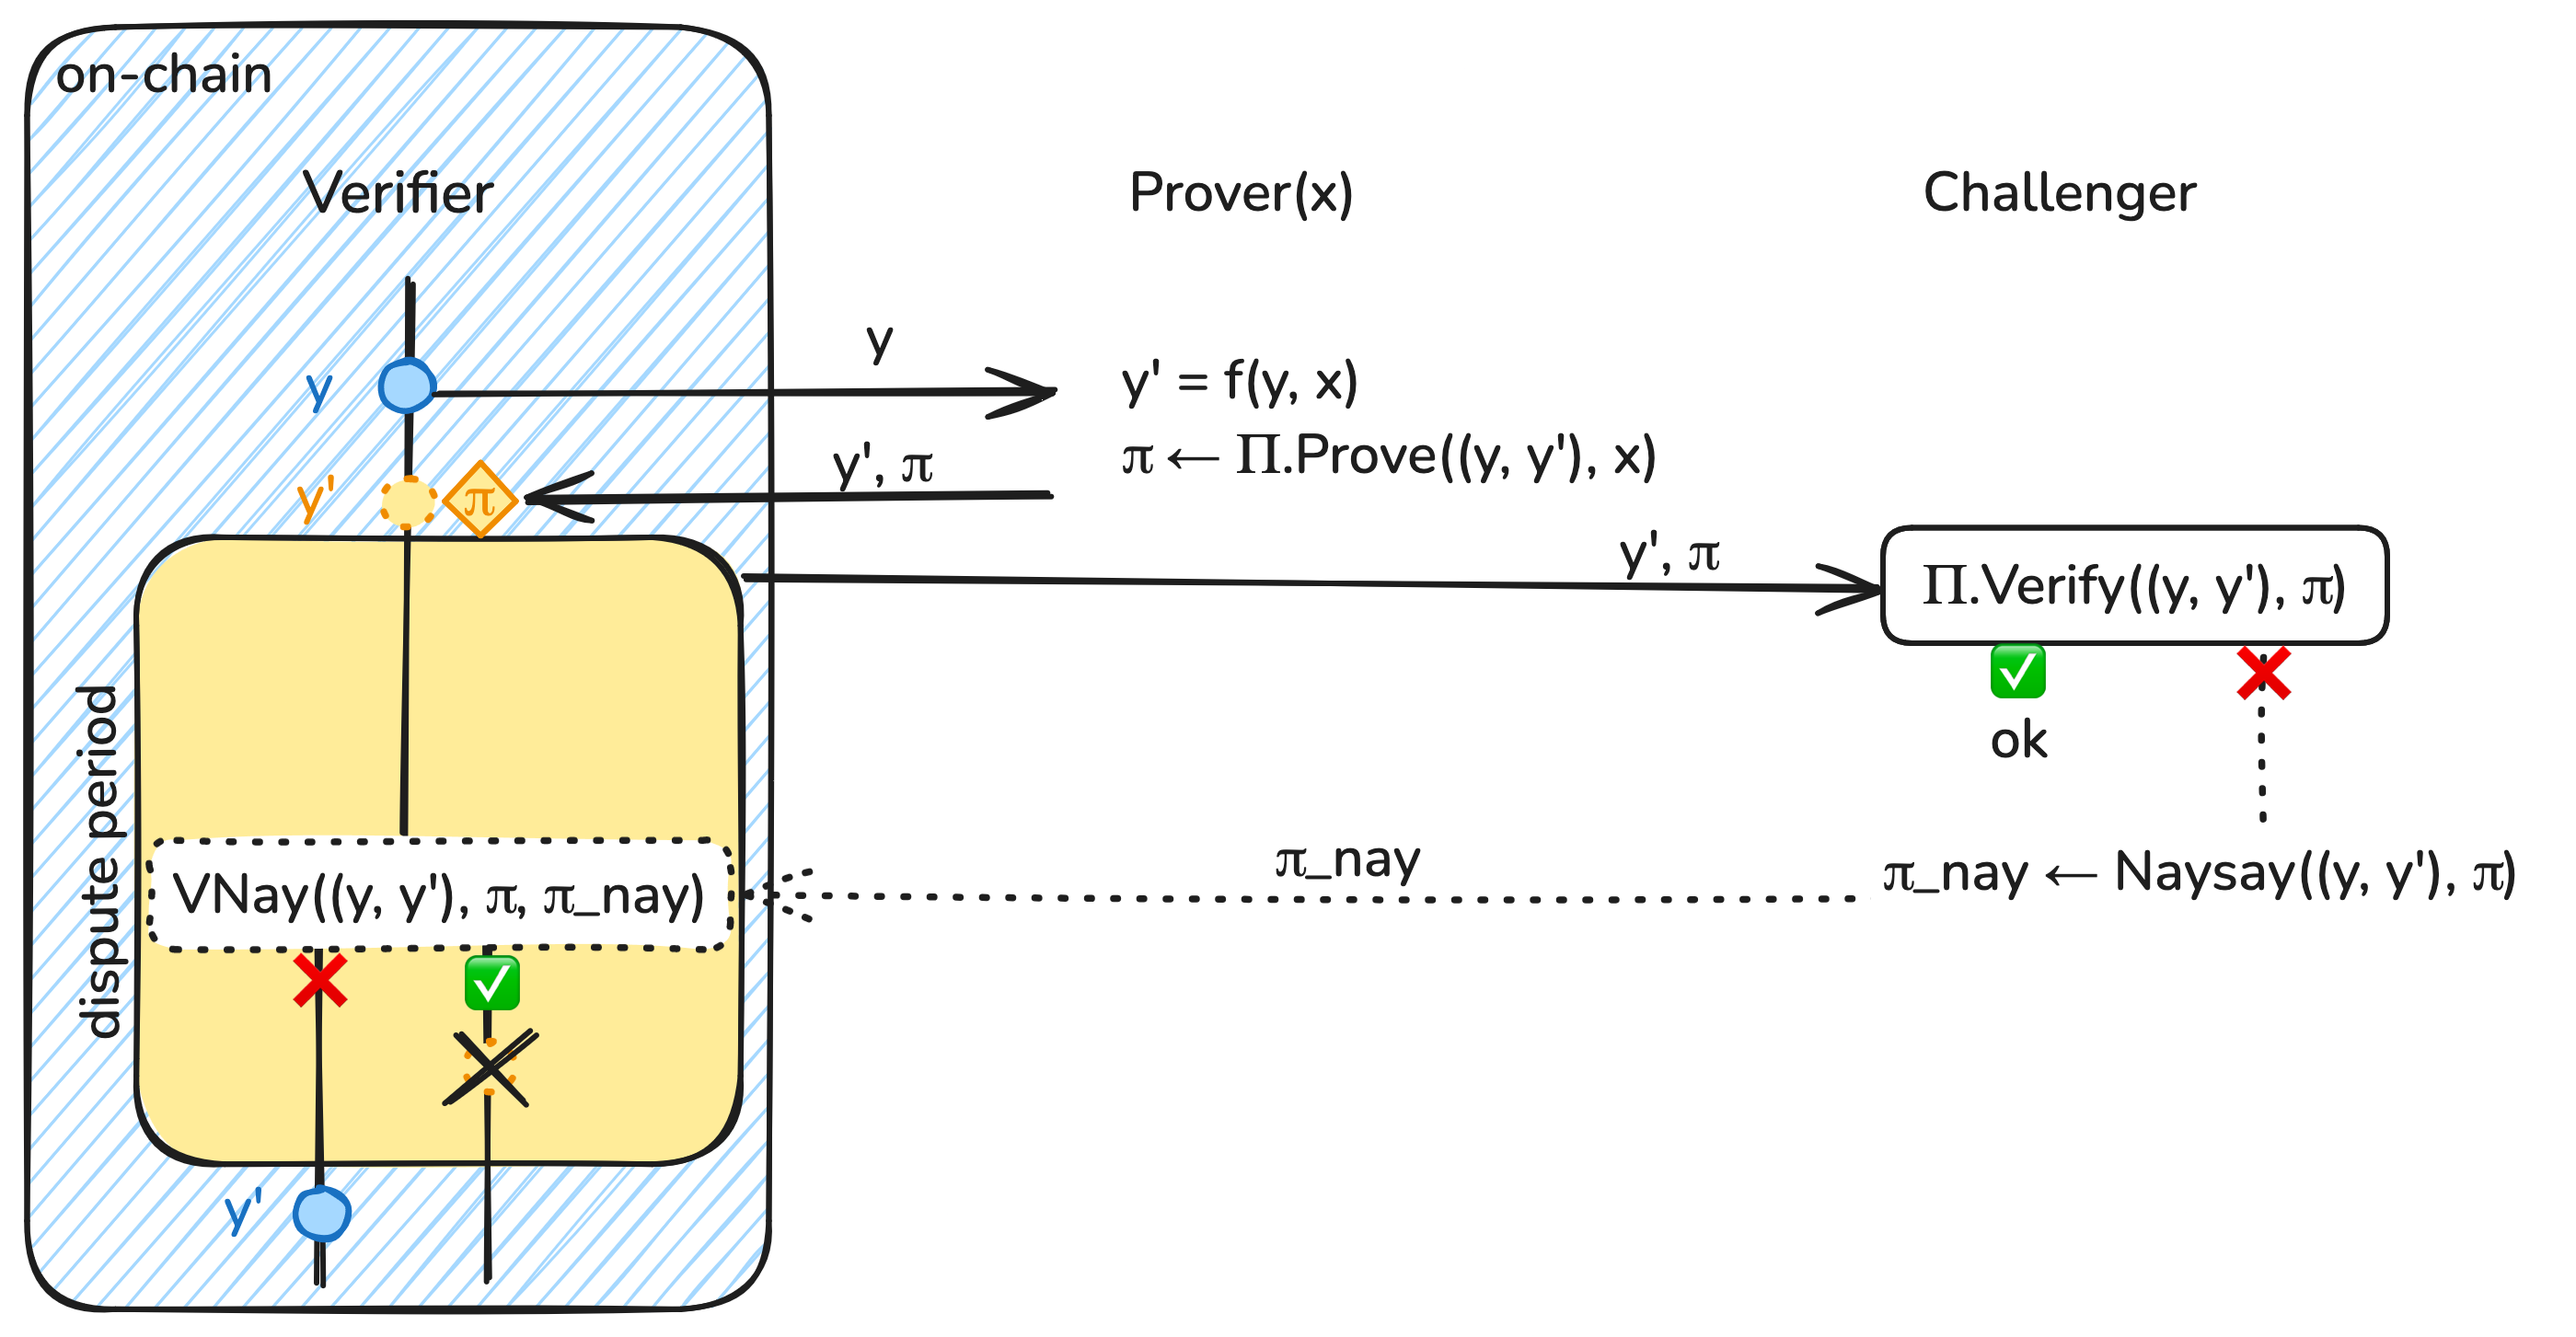
\includegraphics[width=\textwidth]{naysayer/figs/naysayer.png}
    \caption{\textbf{The naysayer proof approach.} As in VC, the off-chain prover computes $y' = f(y, w)$ and $\pi$, which it posts on-chain. This time, the proof is \emph{not} verified on-chain, but is provisionally accepted while waiting for the challenge period to pass. Any party can verify $\pi$ off-chain and, if it fails, issue a challenge by creating a naysayer proof $\pi_\nay$. The on-chain verifier checks any submitted naysayer proofs, and if they pass, it rejects the claimed result $y'$. If the challenge period elapses without any successful naysaying, $y'$ is accepted.}
    \label{fig:naysayer}
 \end{figure}

This state of affairs motivates us to propose a new paradigm called \emph{naysayer proofs} (\Cref{fig:naysayer}). In this paradigm, the verifier (e.g., a rollup smart contract) optimistically accepts a submitted proof without verifying its correctness. Instead, any observer can check the proof off-chain and, if needed, prove its \emph{incorrectness} to the verifier by submitting a \emph{naysayer proof}. The verifier then checks the naysayer proof and, if it is correct, rejects the original proof.
Otherwise, if no party successfully naysays the original proof before the end of the challenge period, the original proof is accepted.
To deter denial of service, naysayers may be required to post collateral, which is forfeited if their naysayer proof is incorrect.

This paradigm potentially saves the verifier work in two ways. 
First, in the optimistic case, where the proof is not challenged, the verifier does no work at all (just like the related fraud proof paradigm; see \Cref{sec:naysayer_related}). We expect this to almost always be the case in practice. Second, even in the pessimistic case, we will see below that checking the naysayer proof can be much more efficient than checking the original proof.
In other words, the naysayer acts as a helper to the verifier by reducing the cost of the verification procedure in fraudulent cases. At worst, checking the naysayer proof is equivalent to verifying the original proof (this is the trivial naysayer construction).

Naysayer proofs enable other interesting trade-offs. 
% for instance, %for a proof system with transparent setup and large proofs, the \naysayer proof could be instantiated generically using a short proof system with trusted setup (e.g., \cite{groth16}), or using a lower security level. 
For instance, naysayer proofs can be instantiated with a lower security level than the original proof system.
This is because a violation of the naysayer proof system's soundness undermines only the \emph{completeness} of the original proof system. %, but not its soundness. 
For an application like a rollup service, this would result in a loss of liveness; importantly, the rollup users' funds would remain secure. 
Liveness could be restored by falling back to full proof verification on-chain.

%Move this to later? Conclusion?
%The naysayer paradigm introduces a new set of criteria for evaluating the efficiency of proof systems. Previously, developers were solely focusing on the proof size and verification cost of a proof system; this paradigm allows one to instead optimize for a proof system's proof size \emph{and its accompanying naysayer proof size and verification cost}. We further detail the implications of these new selection criteria in~\Cref{sec:evaluation}.

We will formally define naysayer proofs in~\Cref{sec:naysayer_def} and show that every succinct proof system has a logarithmic-size and constant-time naysayer proof. Before that, we discuss related work in \Cref{sec:naysayer_related} and define our system model in more detail in \Cref{sec:naysayer_model}.
In~\Cref{sec:naysayer_apps}, we construct naysayer proofs for four concrete proof systems and evaluate their succinctness. % in comparison with verifying the original proof. 
We discuss storage considerations in \Cref{sec:naysayer_storage} and conclude with some open directions in~\Cref{sec:naysayer_extensions}.
\subsection{Related Work}
\label{sec:naysayer-related}

\begin{table}[t]
    \setlength\tabcolsep{0.5em}
    \centering
    \makebox[\linewidth]{
    \begin{tabular}{lcccc}
    \toprule
                                   & VC       & fraud proof       & fraud proof       & naysayer proof \\
                                   &           &   (interactive)   & (non-interactive) &                \\\midrule
        No optimistic assumption   & \yes      & \no               & \no               & \no            \\
        Non-interactive            & \yes      & \no               & \yes              & \yes           \\
        Off-chain $f$  & \yes       & \yes              & \halfcirc             & \yes           \\
        Off-chain $\Pi.\vrfy$  & \no       & -             & -            & \yes           \\
        Witness-independent challenge& \yes    & \no              & \no               & \yes           \\
        Witness-independent resolution& \yes    & \halfcirc              & \no               & \yes           \\
        No $\Pi.\prove$     & \no       & \yes             & \yes              & \no\\
        \bottomrule
    \end{tabular}}
    \caption{Trade-offs between VC, fraud proofs, and naysayer proofs.}
    \label{tab:comparison}
\end{table}

A concept related to the naysayer paradigm is \emph{refereed delegation}~\cite{STOC:FeiKil97}. The idea has found widespread adoption~\cite{ARXIV:TeuRei19,USENIX:KGCWF18} in the form of ``fraud proofs'' or ``fault proofs'' as used in \emph{optimistic rollups}~\cite{ethereum_optimistic,arbitrum_nitro,optimism_rollup}. Like naysayer proofs, fraud proofs work under an optimistic assumption, i.e., a computation is assumed to be correct unless some party challenges it. In case of a challenge, a dispute resolution process ensues between the \emph{challenger} and the \emph{defender}. The parties engage in a \emph{bisection protocol} to locate a single step of the computation whose result they disagree on, and that step is re-executed on-chain to resolve the dispute. 
To non-interactively resolve disputes, the full computation can instead be re-executed by the on-chain verifier.

%Commented out for flow and space
%To improve usability and modularity, researchers have even suggested using succinct proofs of the disputed computation or computation step, replacing the potentially costly on-chain re-execution with proof verification~\cite{buckland_fraudproofs}.

% https://medium.com/@cpbuckland88/fraud-proofs-and-virtual-machines-2826a3412099
% https://www.alchemy.com/overviews/optimistic-rollups

% One major difference between naysayer proofs and fraud proofs is that the latter, despite the name, is not actually a proof system, nor does it depend on any proof system. Instead, a fraud proof is simply an intent to dispute the correctness of some computation (state transition). An interactive process then takes place between the disputing party and the prover to narrow down the particular step of the \emph{prover's computation} which gave rise to the divergence.
We compare classic verifiable computation, fraud proofs, and our new approach in \Cref{tab:comparison}. \noemi{Discuss table here. Note that VC and naysayers require running (cost-intensive) underlying prover, something which fraud proofs avoid.}
At a high level, in the fraud proof paradigm, a ``prover'' performs a provisionally accepted computation without any proof of correctness. Any party can then challenge the correctness of the prover's \emph{computation}. %, potentially by specifying the disputed step of the computation.
In the naysayer paradigm, by contrast, the prover supplies a proof with the computation output, which is provisionally accepted. Any party can then challenge the correctness of the \emph{proof}. %, potentially by specifying the disputed step of the \emph{verification} computation. 
The naysayer approach offers significant speedups since the verifier's circuit is typically much smaller than the original computation. 
Note that there is a slight semantic difference: fraud proofs can definitively show that the computation output is incorrect. In contrast, naysayer proofs can only show that the accompanying proof is invalid---the computation itself may have been correct.

Furthermore, for fraud proofs, the full computation input (the witness) must be made available to the verifier and potential challengers. %and the verifier must be made available to the verifier to settle the dispute. 
Naysayer proofs, on the other hand, 
% are completely stateless to verify:
can be verified using only the statement and proof. 
%\noemi{We have referred to this as ``stateless'', but it's more like no \emph{private} state (i.e. witness) --- is this a standard interpretation of ``stateless'' or might using that word lead to confusion?}
%the on-chain verifier only needs the statement and the proof to check that the proof verifies, and both of these are already available on-chain.
Hence, naysayer proofs work naturally with zero-knowledge proofs.
This can also lead to crucial savings if the witness is very large %as in many cases, the witness is extremely large and, therefore, costly to store on-chain 
(e.g., transaction data for a rollup).

The fraud proof design pattern has been applied in an application-specific way in many blockchain applications besides optimistic rollups, including the Lightning Network~\cite{PooDry16}, Plasma~\cite{PooBut17}, cryptocurrency mixers~\cite{EPRINT:SNBB19}, and distributed key generation~\cite{EPRINT:SJSW19}. We view naysayer proofs as a drop-in replacement for the many application-specific fault proofs, offering an alternative which is both more general and more efficient.


\section{Model}\label{sec:naysayer_model}

There are three entities in a naysayer proof system. We assume that all parties can read and write to a public bulletin board (e.g., a blockchain). Fix a function $f: \mathcal{X} \times \mathcal{W} \to \mathcal{Y}$ and let $\Lang_f$ be the language $\{(x, y): \exists \witness \suchthat y = f(x, \witness)\}$. Let $\Rel_f = \{((x, y), \witness)\}$ be the corresponding relation. We assume $f,x$ are known by all parties. When $f : \mathcal{Y} \times \mathcal{W} \to \mathcal{Y}$ is a state transition function with $y' = f(y, w)$, this corresponds to the rollup scenarios described above.
\begin{description}
    \item[Prover] The prover posts $y$ and a proof $\pi$ to the bulletin board claiming $(x,y) \in \Lang_f$. 
    \item[Verifier] The verifier does not directly verify the validity of $y$ or $\pi$, rather, it waits for time $T_{\nay}$.
    If no one naysays $(y, \pi)$ within that time, the verifier accepts $y$. In the pessimistic case, a party (or multiple parties) naysay the validity of $\pi$ by posting proof(s) $\pi_{\nay}$. The verifier checks the validity of each $\pi_{\nay}$, and if any of them pass, it rejects $y$.
    \item[Naysayer] If $\vrfy(\crs, (x,y),\pi)=0$, then the naysayer posts a naysayer proof $\pi_{\nay}$ to the public bulletin board before $T_{\nay}$ time elapses.
\end{description}

Note that, due to the optimistic paradigm, we must assume a synchronous communication model: in partial synchrony or asynchrony, the adversary can arbitrarily delay the posting of naysayer proofs, and one cannot enforce soundness of the underlying proofs. 
% Synchrony is already assumed by most deployed consensus algorithms, e.g., Nakamoto consensus~\cite{Nakamoto08}. \noemi{Ethereum's consensus uses Gasper~\cite{ARXIV:BHKPQR20}, which requires only asynchrony, or partial synchrony for probabilistic liveness (see \S2.6 therein).} \noemi{note we require synchrony, not liveness, which is weaker since it can be (probabilistically) achieved under asynchrony}
Furthermore, we assume that the public bulletin board offers censorship-resistance, i.e., anyone who wishes to write to it can do so successfully within a certain time bound. Finally, we assume that there is \emph{at least one honest party} who will submit a naysayer proof for any invalid $\pi$.
\subsection{Formal Definitions}\label{sec:naysayer_def}

Next, we introduce a formal definition and syntax for naysayer proofs. A naysayer proof system $\Pi_{\nay}$ can be seen as a ``wrapper'' around an underlying proof system $\Pi$. For example, $\Pi_{\sf nay}$ defines a proving algorithm $\Pi_{\nay}.\prove$ which uses the original prover $\Pi.\prove$ as a subroutine.

\begin{definition}[Naysayer proof]\label{def:naysayer_proof}
Given a non-interactive proof system $\Pi = (\setup, \prove, \vrfy)$ for a NP language $\Lang$, the naysayer proof system corresponding to $\Pi$ is a tuple of PPT algorithms $\Pi_{\nay} = (\setup, \prove,\allowbreak \naysay, \vrfynay)$ defined as follows:
    \begin{description}
        \item[$\setup(\secparam, \naysecparam) \randout (\crs,\crs_{\nay})$:] Given (potentially different) security parameters $\secparam$ and $\naysecparam$, output two common reference strings $\crs$ and $\crs_{\nay}$. This algorithm may use private randomness.
        \item[$\prove(\crs, x, \witness) \to \pi'$:] Given a statement $x$ and witness $\witness$ such that $(x,\allowbreak \witness) \in \Rel$, 
        % compute $\pi \gets \Pi.\prove(\crs, x,w)$ and a commitment $\com$ to the evaluation trace of $\Pi.\vrfy(\crs, x, \pi)$. 
        output $\pi' = (\pi, \aux)$, where $\pi \gets \Pi.\prove(\crs, x, \witness)$.
        \item[$\naysay(\crs_\nay, (x,\pi'), \td_{\nay}) \rightarrow \pi_{\nay}$:] Given a statement $x$ and values $\pi' = (\pi,\allowbreak \aux)$ where $\pi$ is a (potentially invalid) proof that $x \in \Lang$ using the proof system $\Pi$, output a naysayer proof $\pi_\nay$ disputing $\pi$. This algorithm may also make use of some (private) trapdoor information $\td_\nay$.
        \item[$\vrfynay(\crs_\nay, (x,\pi'), \pi_\nay) \rightarrow \{0, \perp\}$:] Given a statement-proof pair $(x,\allowbreak \pi')$ and a naysayer proof $\pi_\nay$ disputing $\pi'$, output a bit indicating whether the evidence is sufficient to reject (0) or inconclusive ($\perp$).
    \end{description}
\end{definition}

%Naysayer proofs are most interesting if $\vrfynay$ takes less time than directly verifying the proof $\pi$, i.e., running the $\vrfy$ algorithm. 
A trivial naysayer proof system always exists in which $\pi_\nay = \top$, $\pi' = (\pi, \perp)$, and $\vrfynay$ simply runs the original verification procedure, outputting $0$ if $\Pi.\vrfy(\crs, x, \pi) = 0$ and $\perp$ otherwise.
We say a proof system $\Pi$ is \emph{efficiently naysayable} if there exists a corresponding naysayer proof system $\Pi_{\nay}$ such that $\vrfynay$ is asymptotically faster than $\vrfy$. If $\vrfynay$ is only concretely faster than $\vrfy$, we say $\Pi_{\nay}$ is a \emph{weakly efficient} naysayer proof. Note that some proof systems already have constant proof size and verification time~\cite{EC:Groth16,C:Schnorr89} and therefore can, at best, admit only weakly efficient naysayer proofs. 
Moreover, if $\td_\nay = \perp$, we say $\Pi_\nay$ is a \emph{public} naysayer proof (see \Cref{sec:naysayer_apps} for an example of a non-public naysayer proof). 

\begin{definition}[Naysayer completeness]
    Given a proof system $\Pi$, a naysayer proof system $\Pi_{\nay} = (\setup, \prove, \naysay, \vrfynay)$ is \emph{complete} if, for all honestly generated $\crs, \crs_{\nay}$ and all values of $\aux$,\footnotemark
    % all statements $x$, all invalid proofs $\pi$, and all corresponding auxiliary information $\witness_{\nay}$, 
    given an invalid statement-proof pair $(x,\pi)$, $\naysay$ outputs a valid naysayer proof $\pi_{\nay}$. That is, for all $\secpar, \naysecpar \in \NN$ and all $\aux,x,\pi$,
\footnotetext{We do not place any requirement on $\aux$.}
\begin{equation*}
    \Pr\left[
        \vrfynay(\crs_{\nay}, (x,(\pi, \aux)), \pi_{\nay})=0 
        \middle| 
        \begin{array}{c}
            (\crs, \crs_{\nay}) \gets \setup(\secparam, \naysecparam)~\land\\
            \Pi.\vrfy(\crs, x,\pi) \neq 1~\land\\
            \pi_{\nay} \gets \naysay(\crs_{\nay}, (x, (\pi, \aux)), \perp)
        \end{array}
    \right] = 1.
\end{equation*}
% \noemi{Note this means completeness is only guaranteed to hold if you do not use a trapdoor... is this a problem? Edit: no, more like you can always naysay even without trapdoor}
\end{definition}

\begin{definition}[Naysayer soundness] Given a proof system $\Pi$, a naysayer proof system $\Pi_{\nay}$ is \emph{sound} if, for all PPT adversaries $\adv$, and for all honestly generated $\crs, \crs_\nay$, all $(x,w) \in \Rel_\Lang$, and all correct proofs $\pi'$, $\adv$ produces a passing naysayer proof $\pi_{\nay}$ with at most negligible probability. That is, for all $\secpar, \naysecpar \in \NN$, and all $\td_\nay$,
\begin{equation*}
    \Pr\left[
        \vrfynay(\crs_{\nay}, (x,\pi'), \pi_{\nay})=0 
        \middle| 
        \begin{array}{c}
            (\crs, \crs_\nay) \gets \setup(\secparam, \naysecparam)~\land\\
            % \Pi.\vrfy(\crs, x,\pi)=1~\land\\
            (x,w) \in \Rel_\Lang~\land
            \pi' \gets \prove(\crs, x, w)~\land\\
            \pi_\nay \gets \adv(\crs_\nay, (x, \pi'), \td_\nay)
        \end{array}
    \right] \leq\negl[\naysecpar].\footnotemark
\end{equation*}
\footnotetext{If we assume $\aux$ is computed correctly, the second line of the precondition can be simplified to see that $\Pi_\nay$ is a sound proof system for the language $\Lang_\nay = \{(x,\pi) : x \notin \Lang ~\lor~ \Pi.\vrfy(\crs, x, \pi) \neq 1 \}$.}
\end{definition}

Next, we show that every proof system has corresponding naysayer proof system with a logarithmic-sized (in the size of the verification circuit) naysayer proofs and constant verification time (i.e., a succinct naysayer proof system). %We follow the blueprint of~\cite{FOCS:FeiLapSha90}.

\begin{lemma}\label{lemma:naysayingCSAT}
    A claimed satisfying assignment for a circuit $C: \mathcal{X} \to \{0,1\}$ on input $x \in \mathcal{X}$ is efficiently naysayble. That is, if $C(x) \neq 1$, there is an $O(\log{\sizeof{C}})$-size proof of this fact which can be checked in constant-time, assuming oracle access to the wire assignments of $C(x)$.
    % For every NP language $\Lang$ with relation $\Rel_\Lang$, \todo{change to CSAT specifically}
    % assuming a binding commitment scheme with constant-size openings, 
    % there exists a naysayer proof system $\Pi_{\nay}$ with logarithmic-sized proofs $\pi_{\nay}$ and constant-time verifier.
\end{lemma}
\begin{proof}
    % For any NP language $\Lang$, there exists a non-interactive proof system $\Pi = (\setup, \prove, \vrfy)$ for $\Rel_\Lang$ where $\vrfy(\crs, \cdot, \cdot)$ can be represented as a boolean circuit $C$ of size $\mathsf{poly}(\lvert x \rvert)$~\cite{C:LapSha90}. Recall that for all $(x,w) \in \Rel_\Lang$ and $\crs \gets \Pi.\setup(\secparam)$, by correctness, we have that if $\pi' \gets \Pi.\prove(\crs, x, w)$ then $C(x,\pi') = 1$. Therefore, if there is some gate of $C$ for which the wire assignment is inconsistent, then the proof $\pi'$ is incorrect. To naysay, i.e., to show the incorrectness of $\pi'$, the naysayer simply provides the index of the inconsistent gate.
    % Recall that the verifier has access to the wire assignments of $C(x,\pi')$ as part of $\pi$ (see \Cref{def:naysayer_proof}). 
    Without loss of generality, let $C$ be a circuit of fan-in 2. 
    
    If $C(x) \neq 1$, then there must be some gate of $C$ for which the wire assignment is inconsistent. Let $i$ be the index of this gate (note $\sizeof{i} \in O(\log{\sizeof{C}})$). To confirm that $C(x) \neq 1$, a party can re-evaluate the indicated gate $G_i$ on its inputs $a,b$ and compare the result to the output wire $c$. That is, if $G_i(a,b) \neq c$, the verifier rejects the satisfying assignment.
    % The verifier then checks whether the wire assignments of $C(x,\pi')$ are consistent with a correct evaluation of the gate, which is a constant-time operation assuming constant-time indexing into the wire assignments. 
    % Furthermore, the naysayer proof consists only of the gate index, which is logarithmic in the circuit size, i.e., succinct.
\end{proof}

\begin{theorem}\label{thm:naysayer}
    Every efficient proof system $\Pi$ (i.e., with a polynomial-time verification algorithm) has a succinct naysayer proof.
\end{theorem}
\begin{proof}
Given any proof system $\Pi$, the evaluation of $\Pi.\vrfy(\crs,\cdot,\cdot)$ can be represented as a circuit $C$. (We assume this circuit description is public.) 
% Let $\COM$ be a deterministic, binding commitment scheme with succinct openings and $\com \gets \COM.\Commit(\Pi.\vrfy(\crs,x,\pi))$ be a commitment to the verification trace of a statement-proof pair $(x,\pi)$. 
Then the following is a complete and sound naysayer proof system $\Pi_\nay$:

\begin{description}
    \item[$\setup(\secparam, \naysecparam)$:] Output $\crs \gets \Pi.\setup(\secparam)$ and $\crs_\nay := \varnothing$.
    % $\crs_\nay \gets \COM.\setup(\naysecparam)$.
    \item[$\prove(\crs, x, w) \to \pi'$:] Let $\pi \gets \Pi.\prove(\crs, x, w)$ and $\aux$ be the wire assignments of $\Pi.\vrfy(\crs, x, \pi)$. Output $\pi' = (\pi, \aux)$.
    \item[$\naysay(\crs_\nay, (x, \pi'), \td_\nay)$:] Parse $\pi' = (\pi, \aux)$\footnote{if $\sizeof{\aux}$ is larger than the number of wires in $C$, truncate it to the appropriate length} and output $\pi_\nay := \top$ if $\aux = \aux' \concat 0$. Otherwise, evaluate $\Pi.\vrfy(\crs, x, \pi)$. If the result is not 1, search $\aux$ to find an incorrect wire assignment for some gate $G_i \in C$. %(if $\aux = \aux' \concat 0$, let $i = \sizeof{C}-1$). 
    Output $\pi_\nay := i$. \todo{asymptotic runtime of $\naysay$? Depends on how we define runtime of $\Pi.\vrfy$.}
    \item[$\vrfynay(\crs_\nay, (x, \pi'), \pi_\nay)$:] Parse $\pi' = (\cdot, \aux)$ and $\pi_\nay = i$. If $\aux = \aux' \concat 0$, output 0, indicating rejection of the proof $\pi'$. Otherwise, obtain the values $\mathsf{in},\mathsf{out} \in \aux$ corresponding to the gate $G_i$ % (recall that the circuit description is public so $G_i$ is known)
    and check $G_i(\mathsf{in}) \stackrel{?}{=} \mathsf{out}$. If the equality does not hold, output $\perp$; else output 0.
\end{description}

Completeness (if a $\pi$ fails to verify, we can naysay $(\pi, \aux)$) follows by \Cref{lemma:naysayingCSAT}. If $\Pi.\vrfy(\crs,x,\pi) \neq 1$, then we have two cases: If $\aux$ is consistent with a correct evaluation of $\Pi.\vrfy(\crs, x, \pi)$, either $\aux = \aux' \concat 0$ (and $\vrfynay$ rejects) or we can apply the lemma to find an index $i$ such that $G_i(\mathsf{in}) \neq \mathsf{out}$ for $\mathsf{in}, \mathsf{out} \in \aux$, where $G_i \in C$. Alternatively, if $\aux$ is not consistent with a correct evaluation, there must be some gate (with index $i'$) which was evaluated incorrectly, i.e., $G_{i'}(\mathsf{in}) \neq \mathsf{out}$ for $\mathsf{in}, \mathsf{out} \in \aux$.

Soundness follows by the completeness of $\Pi$. If $(x,w) \in \Rel_\Lang$ and $\pi' = (\pi, \aux)$ is computed correctly, completeness of $\Pi$ implies $\Pi.\vrfy(\crs, x, \pi) = 1$. Since $\aux$ is correct, it follows that $\aux \neq \aux \concat 0$ and $G_i(\mathsf{in}) = \mathsf{out}$ for all $i \in \sizeof{C}$ and corresponding values $\mathsf{in},\mathsf{out} \in \aux$. Thus there is no index $i$ which will cause $\vrfynay(\crs_\nay, (x, \pi'), i)$ to output 0.

Succinctness of $\pi_\nay$ follows from the fact that $i \in O(\sizeof{\Pi.\vrfy(\crs, \cdot, \cdot)}) \in O(\log{\sizeof{w}})$ (by the succinctness \todo{define and check} of $\Pi$). Furthermore, it is clear to see that the runtime of $\vrfynay$ is constant.
\end{proof}

The proof of \Cref{thm:naysayer} gives a generic way to build a succinct naysayer proof system for any succinct proof system $\Pi$. \todo{Mention zkVMs} Notice that although the syntax gives $\pi' = (\pi, \aux)$ as an input to the $\vrfynay$ algorithm, in the generic construction the algorithm does not make use of $\pi$. Thus, if the naysayer rollup from \Cref{fig:naysayer} were instantiated with this generic construction, $\pi$ would not need to be posted on-chain since the on-chain verifier (running the $\vrfynay$ algorithm) will not use this information. In fact, the verifier wouldn't even need most of $\aux$---only the values corresponding to the gate $G_i$, which is determined by $\pi_\nay$. Thus, although $\pi'$ must be available to all potential naysayers, only a small (adaptive) fraction of it must be accessible on-chain. We describe in \Cref{sec:naysayer_storage} how to leverage this insight to reduce the storage costs of a naysayer rollup. First, in \Cref{sec:naysayer_apps}, we show application-specific naysayer constructions which are more efficient than the generic naysayer proof.

% \paragraph{Naysaying a zkVM.} 
% \noemi{Given an underlying zkVM, you can define a corresponding naysayer proof based on the $\mathsf{zkVM}.\vrfy$ circuit --- with the rise of zkVMs, should mention this. This is still ``application-specific'', since the naysayer proof depends on what zkVM is used (on its design/proof system). But in practice it's more ``general-purpose''. However, I think naysayer proofs are inherently application-specific since they rely on the structure of the verification circuit. But if we, as an area, start using only a few common verification circuits (e.g., adopting a few standard zkVMs), then the naysayer proof system can be reused.}
% 
% \noemi{update: not sure if it makes sense to talk about a $\mathsf{zkVM}.\vrfy$ circuit---they're generally just some proof system's verification procedure, e.g. the RISC Zero zkVM is running a STARK. Just talk about general naysaying by committing to a verification trace---and mention zkVMs somewhere as an example---then talk about particular languages where the verification trace is not needed because the structure is repetitive (i.e., conjunctions).}

\subsection{Applications}\label{sec:naysayer_apps}

The naysayer proof paradigm is generally applicable for proof systems with multi-round amplification, repetitive structure (e.g., multiple bilinear pairing checks~\cite{EPRINT:GabWilCio19}), or recursive reduction (e.g., Pietrzak's proof of exponentiation~\cite{ITCS:Pietrzak19b}). In this section, we highlight three example constructions of naysayer proofs.

\subsubsection{FRI Polynomial Commitment Scheme}\label{sec:fri_example}

The FRI polynomial commitment scheme~\cite{EPRINT:BBHR18} is used as a building block in many non-interactive proof systems, including STARKs~\cite{STOC:BCGT13}.
Below, we describe only the parts of FRI relevant to our discussion. The FRI commitment to a polynomial $p(x)\in\mathbb{F}^{\leq d}[X]$ is the root of a Merkle tree with $\rho^{-1}d$ leaves. 
Each leaf is an evaluation of $p(x)$ on the set $L_0\subset\mathbb{F}$, where $\rho^{-1}d=\vert L_0\vert\ll\vert\FF\vert$, for $0<\rho<1$. We focus on the verifier's cost in the opening proof of the FRI polynomial commitment scheme as applied in the STARK IOP. Let $\delta$ be a parameter of the scheme such that $\delta\in(0,1-\sqrt{\rho})$. The prover sends the verifier $\log_2(\vert L_0\vert)$ messages. The FRI opening proof's verifier queries the prover's each message $\secpar/\log_2(1/(1-\delta))$ times to ensure $2^{-\secpar}$ soundness error. In each query, the verifier needs to check a Merkle-tree authentication path consisting of $\mathcal{O}(\log_2(\rho^{-1}d))$ hashes. Therefore, the overall STARK proof consists of $\mathcal{O}(\secpar\log_2(\rho^{-1}d)/\log_2(1/(1-\delta)))$ hashes. 

The overall STARK proof is invalid if any of the individual Merkle proofs is invalid. Therefore a straightforward naysayer proof $\pi^{\mathsf{FRI}}_{\nay}=(i,z_{i})$ need only point to the $i$th node in one of the Merkle proofs, where the hash values of the children nodes $x,y$ and their parent node $z\neq H(x,y)$ do not match in one of the incorrect Merkle authentication paths. The naysayer verifier only needs to compute a single hash evaluation $H(x,y)=z_{i}$ and check $z_{i}\neq z$. Thus, the naysayer proof for FRI has constant-size and can be verified in constant-time. 

\subsubsection{Post-quantum Signature Schemes}
With the advent of account abstraction~\cite{accountabstraction}, Ethereum users can define their own preferred digital signature schemes, including post-quantum signatures as recently standardized by NIST~\cite{CCS:BHKNRS19,TCHES:DKLLS18,NISTPQC:FALCON22}.
In all known schemes, %\joe{check this} 
post-quantum signatures or public keys are substantially larger than their classical counterparts.  Since post-quantum signatures are generally expensive to verify on-chain, they are prime candidates for the naysayer proof paradigm.

\paragraph{CRYSTALS-Dilithium~\cite{TCHES:DKLLS18}.} The verifier of this scheme checks that the following holds for signature $\sigma=(\mathbf{z},c)$, public key $\mathit{pk}=(\mathbf{A},\mathbf{t})$, and message $M$:
\begin{equation}\label{eq:crystals_verifier_check}
    \forall i: \lVert z_i\rVert_{\infty}\leq C\land \mathbf{A}\mathbf{z}-c\mathbf{t} = \mathbf{w} \land c=H(M\vert\vert \mathbf{w}),
\end{equation}
where $C$ is a constant, $\mathbf{A}\in R^{k\times l}_q$, and $\mathbf{z},\mathbf{t},\mathbf{w}\in R^{k}_q$ for the polynomial ring $R_q:=\mathbb{Z}_q[x]/(X^{256}+1)$. Notice that the checks in~\Cref{eq:crystals_verifier_check} are efficiently naysayable. In fact, the naysayer prover must show that the following holds: 
\begin{equation}\label{eq:crystals_naysayer_prover}
    \exists i: \lVert z_i\rVert_{\infty}>C\lor \mathbf{A}\mathbf{z}-c\mathbf{t} \neq \mathbf{w} \lor c\neq H(M\vert\vert \mathbf{w}).
\end{equation}
If the first check fails, then the naysayer prover shows an index $i$ for which the infinity norm of one of the polynomials in $\mathbf{z}$ is large. If the second check fails, then the naysayer prover can point to the $i$th row of the vector $\mathbf{w}$, where matrix-vector multiplication fails and verify only that row. Finally, if the last check fails, then the naysayer verifier just needs to recompute a single hash evaluation.

\paragraph{SPHINCS+~\cite{CCS:BHKNRS19}.} The signature verifier in SPHINCS+ checks several Merkle authentication proofs, requiring hundreds of hash evaluations. A constant-size and -time naysayer proof can be easily devised akin to the naysayer proof described in~\Cref{sec:fri_example}. The naysayer prover simply points to the hash evaluation in one of the Merkle-trees where the signature verification fails. 

\subsubsection{Verifiable Shuffles}\label{sec:verifiable_shuffle_naysayer}
Verifiable shuffles are applied in many (blockchain) applications such as single secret leader election algorithms~\cite{AFT:Boneh20}, mix-nets~\cite{CACM:Chaum81}, cryptocurrency mixers~\cite{EPRINT:SNBB19}, and e-voting~\cite{USENIX:Adida08}. The state-of-the-art proof system for proving the correctness of a shuffle is due to Bayer and Groth~\cite{EC:BayGro12}. Their proof system is computationally heavy to verify on-chain as the proof size is $\mathcal{O}(\sqrt{n})$ and verification time is $\mathcal{O}(n)$, where $n$ is the number of shuffled elements. 

Most shuffling protocols (of public keys, re-randomizable commitments, or ElGamal ciphertexts) admit a succinct naysayer proof if the naysayer knows at least one of the shuffled elements. Let us consider the simplest case of shuffling public keys. We want to prove membership in the following  NP language:
\begin{equation}\label{eq:permlanguage}
    \mathcal{R}_{perm}:=\{(g^{\witness_i},g^{r\cdot \witness_{\sigma(i)}})^{n}_{i=1},g^r;\sigma,r\vert\ \forall i:\witness_i,r\in_{R}\mathbb{F}_p,g\in\mathbb{G},  \sigma\in_{R}\mathsf{Perm}(n)\}, 
\end{equation}
where $\mathsf{Perm}(n)$ is the set of all permutations $f:[n]\rightarrow[n]$.
Suppose the naysayer knows that for $j\in[n]$, the prover did not correctly include $g^{r\cdot \witness_j}$ in the shuffle. The naysayer can prove this by showing that $(g,g^{\witness_j},g^r,g^{r\cdot \witness_j})\in\mathcal{R}_{DH}\land g^{r\cdot \witness_j}\notin (\cdot,g^{r\cdot \witness_{\sigma(i)}})^n_{i=1}$, where $\mathcal{R}_{DH}$ is the language of Diffie-Hellman tuples. One can show that a tuple is a Diffie-Hellman tuple with a proof of knowledge of discrete logarithm equality~\cite{C:ChaPed92}. However, the naysayer must know the discrete logarithm $\witness_j$ to produce such a proof. Unlike our previous examples, which were publicly naysayable, this is a privately naysayable proof since the naysayer algorithm takes auxiliary input $\witness_j$. With the right data structure for the permuted list (e.g., a hash table), both of the above conditions can be checked in constant-time with a constant-size naysayer proof, resulting in exponential savings compared to directly verifying the original Bayer-Groth shuffle proof.

\subsubsection{Evaluation}
We evaluate the asymptotic cost savings for the verifiers in the four examples discussed in~\Cref{sec:naysayer_apps}. Note that naysayer proofs allow an exponential speedup for the verifier for verifiable shuffles and a logarithmic speedup for the FRI polynomial commitment opening proof verifier, see~\Cref{tab:apps_table}. For CRYSTALS-Dilithium, we can only claim weakly efficient naysayer proofs, as there is no asymptotic gap in the complexity in certain branches of the signature verification circuit and the naysayer prover algorithm, cf.~\Cref{eq:crystals_verifier_check,eq:crystals_naysayer_prover}.

%------------------BEGIN Naysayer cost savings TABLE--------------
%-----------------------------------------
\begin{table}[tbh!]
   \centering
   \makebox[\linewidth]{
    \setlength{\belowbottomsep}{6pt}
    \begin{tabular}{l c c c c} 
    \toprule
     & \textbf{FRI Opening} & \textbf{CRYSTALS-D.} & \textbf{SPHINCS+}& \textbf{Shuffle proof} \\ [0.5ex] 
     \midrule
     $\pi$ storage & $\mathcal{O}(\secpar\log^2(d))\mathbb{H}$\ & $\mathcal{O}(\secpar)\FF$\  & $\mathcal{O}(\secpar)\FF$\  & $\mathcal{O}(\sqrt{n})\GG$\  \\ 
     $\vrfy(\pi)$ compute & $\mathcal{O}(\secpar\log^2(d))\mathbb{H}$\ & $\mathcal{O}(\secpar)\FF+1\mathbb{H}$\  & $\mathcal{O}(\secpar)\mathbb{H}$\  & $\mathcal{O}(n)\GG$\  \\\midrule
     $\pi_{nay}$ storage & $1\FF$\ & $1\FF\lor1\FF\lor1\FF$\  & $1\FF$\  & $2\GG+1\FF$\  \\
     ${\sf N}\vrfy(\pi_{nay})$ compute & $1\mathbb{H}$\ & $\mathcal{O}(\secpar)\FF\lor\mathcal{O}(\secpar)\FF\lor1\mathbb{H}$\  & $1\mathbb{H}$\  & $4\GG$\  \\
    \bottomrule
    \end{tabular}
    }
    \caption{Cost savings of the naysayer paradigm for the example applications in~\Cref{sec:naysayer_apps}. In FRI, let $deg(p(x))=d$. For the Bayer-Groth shuffle argument~\cite{EC:BayGro12}, we consider $n$ shuffled public keys (or ciphertexts). $\FF,\GG$ denotes field/group elements or field/group operations, respectively. $\mathbb{H}$ denotes hashing operations. \todo{Can I get some estimated numbers here by looking at the implementations/papers of the underlying schemes, and then just the field/group element sizes in the relevant curves for the naysayer?}}
    \label{tab:apps_table}
   \end{table}
   %--------------------END Naysayer cost savings TABLE--------------
   %-------------------------------------------------
   
\subsection{Storage Considerations}\label{sec:naysayer_storage}

So far, we have assumed that the naysayer verifier can read the instance $x$, the original proof $\pi$ and $\aux$, and the naysayer proof $\pi_\nay$ entirely. A naysayer proof system thus requires increased storage (long-term for $\aux$, and temporary for $\pi_{\nay}$ only in case of a challenge). However, the verifier only needs to compute $\vrfynay$ instead of $\vrfy$. A useful naysayer proof system should therefore compensate for the increased storage by considerably reducing verification costs.

In either case, in blockchain contexts where storage is typically very costly, the approach of storing all data on chain may not be sufficient. Furthermore, as we pointed out previously, the verifier---the only entity which requires data to be stored on-chain in order to access it---does not access all of this data.

Blockchains such as Ethereum differentiate costs between persistent storage (which we can call $S_{\sf per}$) and ``call data'' ($S_{\sf call}$), which is available only for one transaction and is significantly cheaper as a result. Verifiable computation proofs, for example, are usually stored in $S_{\sf call}$ with only the verification result persisted to $S_{\sf per}$.

Some applications now use a third, even cheaper, tier of data storage, namely off-chain \emph{data availability services} ($S_{\sf DA}$), which promise to make data available off-chain but which on-chain contracts have no ability to read. Verifiable storage, an analog of verifiable computation, enables a verifier to store only a short commitment to a large vector~\cite{PKC:CatFio13,C:Merkle87} or polynomial~\cite{AC:KatZavGol10}, with an untrusted storage provider ($S_{\sf DA}$) storing the full values. Individual data items (elements in a vector or evaluations of the polynomial) can be provided as needed to $S_{\sf call}$ or $S_{\sf per}$ with short proofs that they are correct with respect to the stored commitment.  (Ethereum implemented this type of storage, commonly referred to as ``blob data'', using KZG commitments in EIP-4844~\cite{eip4844}.)

This suggests an optimization for naysayer proofs in a blockchain context: the prover posts only a binding commitment $\Commit(\pi')$, which the contract stores in $S_{\sf per}$, while the actual proof $\pi' = (\pi, \aux)$ is stored in $S_{\sf DA}$. We assume that potential naysayers can read $\pi'$ from $S_{\sf DA}$. In the optimistic case, the full proof $\pi'$ is never written to the more-expensive $S_{\sf call}$ or $S_{\sf per}$. In the other case, when naysaying is necessary, the naysayer must send openings of the erroneous elements to the verifier (in $S_{\sf call}$), who checks that these data elements are valid with respect to the on-chain commitment $\Commit(\pi')$ stored in $S_{\sf per}$. Note that most naysayer proof systems don't require reading all of $\pi'$ for verification, so even the pessimistic case will offer significant savings over storing all of $\pi'$ in $S_{\sf call}$. 
% An important future research direction is to investigate this optimized storage model's implications and implementation details.

%Note that in the optimistic case, naysayer proofs fully shift computation and storage (i.e., access to $x, \pi$) from the verifier to the naysayer. In the pessimistic case, the verifier requires slightly increased storage ($x,\pi, \pi_{\nay}$) but only needs to compute $\vfynay$ instead of $\vfy$. A useful naysayer proof system should compensate for the increased storage cost by considerably reducing verification costs.
\subsection{Extensions and Future Work}\label{sec:naysayer_extensions}

In the months since the publication of the original paper~\cite{FC:SerGlaBon24}, naysayer proofs have already received attention from various groups of practitioners hoping to deploy them in production. We see many interesting directions for investigation, both for immediate deployments and to improve our understanding of this new paradigm and its implications.

\begin{description}
    \item[\textbf{Rollup design space.}] Naysayer proofs can be viewed as a way (one of several) of combining two established solutions---verifiable computation and fraud proofs---to offer different tradeoffs. There may be other ways to combine these two paradigms to achieve different tradeoffs which can be more suited to certain application scenarios.
    
    \todo{edit:} Type-2 naysayer proofs are even more efficient in the optimistic case, as the prover \emph{only sends the instance $x$} and no proofs at all, claiming without evidence that $(x,w) \in \Rel_\Lang$ (this is the same as in the fraud proof paradigm). On the other hand, if the prover's assertion is incorrect, i.e., $(x,w) \notin \Rel_\Lang$, then a naysayer prover provides the correct statement $x'$ such that $(x',w) \in \Rel_\Lang$ 
    and a corresponding ``regular'' proof $\pi$ such that $\vrfy(\crs, x', \pi) = 1$. Importantly, $x'$ must correspond to the same witness $w$ (which must be known to the challenger). For example, in the case of rollups, the (public) witness $w$ is the set of transactions in the rollup, and the statement $x = (\mathsf{st}, \mathsf{st}')$ is the updated rollup state after applying the batch $w$. Therefore, an incorrect assertion represents an incorrect application of the update $w$. The correction $x'$ is the result of the proper application of $w$.
    This can be seen as a naysayer proof system where $\pi' = \varnothing$, $\aux_{\nay} = w$, $\pi_{\nay} = (x', \pi_{x'})$, and $\vrfynay$ runs $\Pi.\vrfy(\crs, x', \pi_{x'})$.
    We conjecture that in most applications, in the worst case, type-2 naysayer proofs are more costly than type-1 naysayer proofs (both compute and storage).

    \todo{continue editing from here}

    \item[\textbf{Naysaying zkVMs.}] An emerging trend in zk-rollups are so-called ``zero{\hyp}knowledge virtual machines'', or zkVMs (again, the ``zk'' part may or may not hold). \noemi{This kinda creates an $\aux$ already (not for verification, but for the original computation); basically rephrases the statement as a conjunction of state transitions.}
    \item[\textbf{Other naysayer constructions.}] In our application-specific naysayer constructions, we looked at naysaying proof systems where verification has some repetitive structure. Are there other proof systems which have particularly efficient or useful naysayer proofs? 
    \item[\textbf{Computing $\aux$.}] A drawback of (generic) naysayer proofs is that the prover must additionally run $\Pi.\vrfy$ to create the verification trace $\aux$. Is there a way to separate/outsource this to another party to reduce the added computational burden on a party already spending so much power to compute the proof?
    \item[\textbf{Implementing query access.}] As mentioned in \Cref{sec:naysayer_storage}, a straightforward way to implement efficient and secure query access to $\pi'$ is to assume some secure data availability service (e.g., Ethereum blob data). Are there other approaches to realizing this access trustlessly?
    % blob data (aka trusted KZG) (see \Cref{sec:naysayer_storage}), prover binding+deterministic commitments (?), Merkle trees
    \item[]
\end{description}

\section{On-chain Voting and Auctions}\label{sec:cicada}
\textit{(Parts of this section are taken/adapted from \cite{CTB:GSZB24}.)}

\textit{(Parts of this section are taken/adapted from \cite{EPRINT:GSZB23}.)}

\paragraph{Special Notation} We will use $n$ as the number of users, $m$ as the number of candidates, and $w$ as the maximum weight to be allocated to any one candidate in a ballot/bid ($n,m,w \in \mathbb{N}$). For simplicity and without loss of generality, we assume the user identities are unique integers $i \in [n]$.
We generally use $i \in [n]$ to index users and $j \in [m]$ for candidates.

Auctions and voting are essential applications of Web3. For example, decentralized marketplaces run auctions to sell digital goods like non-fungible tokens (NFTs)~\cite{opensea_auction} or domain names~\cite{ARXIV:XWYLLX21}, while decentralized autonomous organizations (DAOs) deploy voting schemes to enact decentralized governance~\cite{optimismgov}. Most auction or voting schemes currently deployed on blockchains, e.g., NFT auctions on OpenSea or Uniswap governance~\cite{ARXIV:FriMulWat22}, lack bid/ballot privacy. This can negatively influence user behavior, for example, by vote herding or discouraging participation~\cite{FC:ElkLip04,WTSC:GalYou18,FC:SuzYok03}. The lack of privacy can cause surges in congestion and transaction fees as users try to outbid each other to participate, a negative externality for the entire network.

\begin{table*}[tb]
  \centering
  \makebox[\linewidth]{
    \setlength{\tabcolsep}{3pt}
    \setlength{\belowbottomsep}{6pt}
    \begin{tabular}{lccccc} 
    \toprule
    \multirow{2}*{\textbf{Approach}} & \multirow{2}*{No TTPs} & Non-interactive & Everlasting & \multirow{2}*{Practical} \\
      & & voting & privacy & \\
  \midrule 
  MPC~\cite{FC:BDJNPT06,C:AOZZ15}
  & \no & \yes & \yes & \yes \\ 
  ZK proofs~\cite{USENIX:Adida08,maci,plume,rln}
  & \no & \yes & \yes & \yes \\ 
  FHE~\cite{PQCRYPTO:CGGI16,CCS:DLNS17} 
  & \no & \yes & \yes & \no \\
  HE+ZK proofs~\cite{CCS:DLNS17}
  & \no & \yes & \yes & \halfcirc \\ 
  Commit-reveal~\cite{AUSC:FujOkaOht93,WTSC:GalYou18}
  & \yes & \no & \no & \yes \\
  TLPs+HE~\cite{ESORICS:CJSS21} (\Cref{sec:seq_mpc_tlp})
  & \halfcirc & \yes & \no & \yes \\\midrule
  Cicada (this work) 
  & \yes$^*$ & \yes & \halfcirc & \yes \\ 
    \bottomrule
  \end{tabular}
  }
  \caption{Major approaches for tally-private auction/voting schemes. MPC stands for secure multi-party computation. \cite{CCS:DLNS17} aims to be practical but uses lattice-based cryptography, which is not feasible on-chain today. \cite{C:AOZZ15,ESORICS:CJSS21} require a trusted setup but no TTP. 
  The asterisk indicates that our scheme does not inherently require any TTPs (in particular, if the class group HTLP construction (\Cref{sec:htlp-choice}) is used, Cicada has a transparent setup). Everlasting privacy can be added via an extension (\Cref{sec:everlasting_ballot_privacy}).
  }
  \label{tab:approaches}
  \end{table*}
  %------------------------------END Approaches Table---------------------------

Existing private voting protocols~\cite{maci,plume,rln} achieve privacy at the cost of introducing a trusted authority who is still able to view all submissions.
Alternatively, the only private \emph{and} trustless auction in deployment we are aware of~\cite{ARXIV:XWYLLX21} uses a two-round commit-reveal protocol: in the first round, every party commits to their bid, and in the second round they open the commitments and the winner can be determined.
Other protocols relying on more heavyweight cryptographic building blocks have been proposed in the literature.
We summarize the various approaches for private voting and auctions in \Cref{tab:approaches}.
Unfortunately, all of them suffer from at least one of the following limitations, hindering widespread adoption:

\begin{description}
    \item[Interactivity.] Interactivity is a usability hurdle that often causes friction in the protocols' execution. Mandatory bid/ballot reveals are also a target for censorship.     
    %\item[Lack of censorship-resistance]  Voting and auction schemes can be easily censored due to their public nature.
    A malicious party can bribe the block proposers to exclude certain bids or ballots until the auction/voting ends~\cite{ARXIV:PaiResFox23}. %With bid/ballot privacy the cost of censorship can be increased substantially.
    %
    \item[Trusted third party (TTP).] Many protocols~\cite{maci} use a trusted coordinator to tally submissions during the voting/bidding phase. This introduces a strong assumption which is at odds with the trustless ethos of the blockchain ecosystem.
    %
    \item[Inefficiency.] 
    Compute and storage costs are substantial bottlenecks in decentralized applications running on a public blockchain. Some approaches~\cite{PQCRYPTO:CGGI16,CCS:DLNS17} avoid the previous pitfalls by relying on complex cryptographic primitives such as fully-homomorphic encryption (FHE), whose overheads are impractical in the blockchain setting.
    % \item[Inefficiency.] Introducing more complicated cryptographic primitives such as fully-homomorphic encryption (FHE) introduces additional overheads which can incur extra gas fees or at least extra time for all participants.
\end{description}
\subsection{Related Work}

The cryptographic literature on both voting schemes and sealed-bid auctions is enormous, dating to the 1990s. However, most of these schemes are unsuitable for a fully decentralized and trust-minimized setting due to their inefficiency or reliance on trusted parties, i.e., tally authorities, servers running the public bulletin board, auctioneers, etc. Below, we review auction and voting protocols that use a blockchain as the public bulletin board. 

\paragraph{Voting.} 
%Multi-authority schemes' trust assumptions are non-adequate in a decentralized setting~\cite{cramer1998practical}. 
The study of voting schemes for blockchain applications dates to at least 2017, when McCorry et al.~\cite{mccorry2017smart} proposed a ``boardroom'' voting protocol for DAO governance.
The main disadvantage of their protocol is that the entire protocol can be aborted due to a single party. Groth~\cite{groth2005voting} and Boneh et al.~\cite{boneh2023arithmetic} develop techniques to create ballot correctness proofs for various voting schemes. These protocols all have proofs with size linear in the number of candidates. We break this barrier by applying polynomial commitments and assuming a transparent, lightweight pre-processing phase. Applying HTLPs to voting was suggested when they were proposed by Malavolta and Thyagarajan~\cite{malavolta2019homomorphic}. However, they left the details of making such a protocol practical, secure, and efficient to future work. We aim to fill this gap with our techniques for various election types and our EVM implementation.

\paragraph{Auctions.} 
Auctions are a natural fit for blockchains and were suggested as early as 2018~\cite{cryptoeprint:2018/704}, albeit with a \emph{trusted auctioneer}. Bag et al.\ introduced SEAL, a privacy-preserving sealed-bid auction scheme without auctioneers~\cite{bag2019seal}. However, their protocol employs two rounds of communication since they apply the Hao-Zielinski Anonymous Veto network protocol~\cite{hao20062}. Tyagi et al.\ proposed Riggs~\cite{tyagi2023riggs}, a fair non-interactive auction scheme using timed commitments~\cite[\S6]{freitag2021nonmalleable}. This is perhaps the closest work to ours in implementing auctions (but not voting) in a fully decentralized setting using time-based cryptography. However, their design does not utilize homomorphism to combine puzzles, and as a result the gas costs are high. To achieve practicality Riggs relies on an optimistic second round in which users voluntarily open their puzzles. %It is a challenging design in the pessimistic case when users do not open their commitments, i.e., one needs to force-open the commitments. We believe our approach is more practical as one only needs to solve a single (or handful of) TLPs, even in the worst case.
Chvojka et al. suggest a TLP-based protocol for both e-voting and auctions~\cite{chvojka2021versatile}. Their protocol has a per-auction trusted setup. In~\Cref{sec:seq_mpc_tlp}, we propose using HTLPs for distributed setup to reduce the trust assumption, which may be of independent interest.

\paragraph{Time-based cryptography.} 
Time-based cryptography, which uses inherently sequential functions to delay the revelation of information, also has a lengthy history dating to Rivest, Shamir, and Wagner's 1996 proposal of time-lock encryption~\cite{rivest1996time}.
Numerous variants have emerged since then, including timed commitments~\cite{boneh2000timed}, proofs-of-sequential-work~\cite{mahmoody2013publicly}, VDFs~\cite{boneh2018verifiable}, and homomorphic time-lock puzzles~\cite{malavolta2019homomorphic}, which we employ here.
For a recent survey, we refer the reader to Medley et al.~\cite{medley2023sok}. The only practical work we know of taking advantage of HTLPs is Bicorn~\cite{choi2023bicorn}, which builds a distributed randomness beacon with a single aggregate HTLP for an arbitrary number of entropy contributors.

Delay encryption constitutes the most recent development in time-based cryptography. Delay encryption allows time-lock encryption of a message to an identity by combining identity-based encryption with inherently sequential computation. This cryptographic primitive was introduced by Burdges and De Feo~\cite{burdges2021delay}. However, their isogeny-based construction has enormous memory requirements ($\approx 12$\ TiB), making their scheme impractical.

One can emulate time-based cryptography by applying stronger assumptions instead of assuming the sequentiality of repeated modular squaring. McFly~\cite{dottling2023mcfly} and tlock~\cite{gailly2023tlock} build time-lock encryption from threshold trust, i.e., by assuming that a subset of signers intermittently and reliably releases a threshold signature on the current timestamp. Even though this is a stronger assumption, we view this as a promising alternative research direction. For instance, enabling the aggregation of multiple time-lock ciphertexts could make timelock encryption especially suitable for voting and auction applications; aggregation is not currently possible in the aforementioned schemes as they lack any homomorphism. 
Using any resulting homomorphic time-lock encryption schemes to build efficient voting and auction protocols is a further open problem.
We leave these questions to future work. 


% \paragraph{Number packing schemes.} The residue numeral system found application in error correction~\cite{rns_ecc,rns_ecc2}, side-channel resistance~\cite{papachristodoulou2019practical}, and parallelization of arithmetic computations~\cite{rns_neuralnet,bajard2006combining,asif2017high,rns_homomorphicenc}. Using HTLPs in voting gives rise to a natural new application since it simultaneously benefits from packing tuples of integers into a single integer and parallel arithmetic computation over these tuples. \joe{could kill this or move earlier} \noemi{already mention the last part in the packing section, could add the first sentence there too for context (since we kind of call it a ``new'' packing)} \noemi{done}
\subsection{Our Results}
We aim to build voting and auction protocols that possess the following distinguishing features compared to prior work.
\begin{description}
    \item[Trust-minimization.] In our protocols, we do not want to assume (a quorum of) trusted third parties. The cryptographic voting literature extensively applies trusted parties, for example, to operate a public bulletin board or tally votes. The classic tools used in prior work, e.g. (fully) homomorphic encryption, inherently imply a handful of trusted parties to decrypt the ballots/bids. Apart from the liveness and safety of the blockchain consensus, we solely employ standard cryptographic assumptions.

    \item[One-round protocol.] We argue that usability is one of the major challenges of deploying privacy-preserving voting and auction protocols in practice. Multi-round protocols, e.g., commit-reveal-style protocols, have incentive issues and considerable usability hurdles. We solve these pressing issues with efficient one-round protocols.  

    \item[Ballot/bid privacy.] Last but not least, we want to achieve ballot/bid privacy. Our approach naturally provides privacy until the end of the voting/bidding phase. This is sufficient for avoiding selective aborts and censorship, thereby ensuring fairness. Limited privacy can also be a desideratum in certain settings, e.g. in representative democracies where delegates' votes are published to encourage accountability.
    Alternatively, we show in~\Cref{sec:everlasting_ballot_privacy} how we can add everlasting ballot/bid privacy to our protocol without sacrificing our two previously stated goals. 
\end{description}

Coercion-resistance, i.e., the adversary's inability to coerce voters to cast specific ballots demanded by the adversary, is a crucial property of voting schemes. In the privacy-respecting e-voting literature, it is well-known that receipt-freeness (since the voters cannot prove how they voted) implies coercion-resistance~\cite{STOC:BenTui94}. However, we consider receipt-freeness as a non-goal in our protocol design. Still, we sketch an extension to our framework in~\Cref{sec:extension_coercion_resistance}, where we achieve coercion-resistance via a different pathway than receipt freeness. We leave it to future work to achieve the property of receipt freeness for on-chain voting schemes.%\noemi{Mention non-goals (e.g., receipt-freeness)}

We introduce Cicada, a general framework for practical, privacy-preserving, and trust-minimized protocols for both auctions and voting. 
Cicada uses time-lock puzzles (TLPs)~\cite{RivShaWag96} to achieve \emph{privacy and non-interactivity} in a trustless and efficient manner.
A TLP allows a party to ``encrypt'' a message to the future. Specifically, to recover the solution, one needs to perform a computation that is believed to be inherently sequential, with a parameterizable number of steps.
Intuitively, the TLPs play the role of commitments to bids/ballots that any party can open after a predefined time, avoiding the reliance on a second \emph{reveal} round. 

% \paragraph{(Homomorphic) Time-lock puzzles}
% A time-lock puzzle (TLP) allows a party to ``encrypt'' a message to the future. Specifically, to recover the solution, one needs to perform a computation that is believed to be inherently sequential, with a parameterizable number of steps.

% \begin{definition}[Time-lock puzzle~\cite{RSW96}] A time-lock puzzle scheme $\sf TLP$ consists of the following three efficient algorithms:
%     \begin{description}
%         \item[$\mathsf{TLP.Setup}(\secparam, \Ttime) \randout \pparam$.] The (potentially trusted) setup algorithm takes as input a security parameter $\secparam$ and a difficulty (time) parameter $\Ttime$, and outputs public parameters $\pparam$. % (usually a group $\mathbb{G}$ with $\lambda$ bits of security). 
%         % Typically $\mathbb{G}$ is a group of unknown order, e.g., the group $\mathbb{Z}^{*}_N$. 
%         \item[$\mathsf{TLP.Gen}(\pparam, s) \randout Z$.] Given a solution $s\in\ZZ$, the puzzle generation algorithm efficiently computes a time-lock puzzle $Z\in\mathbb{G}$.
%         \item[$\mathsf{TLP.Solve}(\pparam, Z) \rightarrow s$.] Given a TLP $Z$, the puzzle solving algorithm requires at least $\Ttime$ sequential steps to output the solution $s$.
%     \end{description}
% \end{definition}
% Informally, we say that a TLP scheme is \emph{correct} if $\mathsf{TLP.Gen}$ is efficiently computable and $\tlp.{\sf Solve}$ always recovers the original solution $s$ to a validly constructed puzzle. A TLP scheme is \emph{secure} if $Z$ hides the solution $s$ and no adversary can compute $\mathsf{TLP.Solve}$ in fewer than $\Ttime$ steps with non-negligible probability. For the formal definitions, we refer the reader to~\cite{C:MalThy19}.

Since solving a TLP is computationally intensive, ideally, an efficient protocol would require solving only a sublinear number of TLPs (in the number of voters/bidders). Cicada achieves this via \emph{homomorphic} TLPs (HTLPs): bids/ballots encoded as HTLPs can be ``squashed'' into a sublinear number of TLPs. Fully homomorphic TLPs are not practically efficient, but Malavolta and Thyagarajan~\cite{C:MalThy19} introduced efficient additively and multiplicatively homomorphic TLP constructions which we will describe below. This is clearly enough for simple constructions like first-past-the-post (FPTP) voting, but it remained an open problem how to apply HTLPs to realize more complicated auction and voting protocols, e.g., cumulative voting.
% $\htlp$s allow an evaluator to compute a function $f$ homomorphically on TLPs  $Z_0,\dots,Z_k$ to obtain a puzzle $Z^* = f(Z_0,\dots,Z_k)$ such that for the corresponding puzzle solutions $s_0, \dots, s_k, s^*$, it holds that $f(s_0,\dots,s_k)=s^{*}$. Concretely efficient $\htlp$ constructions are known for addition, multiplication, and XOR. These are already powerful building blocks for first-past-the-post, range and approval voting, which only require adding together votes. 
% Linearly homomorphic TLPs are practical by instantiating them with an elegant scheme derived from the Paillier-encryption scheme~\cite{paillier1999public}.
% ~\cite{malavolta2019homomorphic} showed how to conduct private auctions using a fully-homomorphic TLP. Sadly, fully homomomorphic TLPs are currently not practically efficient and therefore are primarily of theoretical interest. They left devising efficient auction and voting protocols using their techniques to future work. 

We show how to use HTLPs to build practically efficient, private, and non-interactive protocols for a special class of auction and voting schemes where the tallying procedure can be expressed as a linear function. We show that this limited class nonetheless includes many schemes of interest.

Moreover, we introduce a novel linear HTLP based on the exponential ElGamal cryptosystem~\cite{EC:CraGenSch97} over a group of unknown order. This construction is more efficient than the Paillier-based construction~\cite{C:MalThy19} for a small solution space $\mathcal{S} \subset \ZZ_N$, i.e., $\mathcal{S} = \{ s : s \in \JJ_N \land\ s \ll N \}$. Here a puzzle $Z$ is constructed as
\begin{equation}\label{eq:exp_elgamalHTLP}
(g^r, h^r y^s) \in (\ZZ_N^*)^2
\end{equation}
where $g,y \sample \ZZ_N^*$ and again $h = g^{2^\Ttime}$. This scheme is only practical for small $\mathcal{S}$ since, in addition to recomputing $h^r$, recovering $s$ requires brute-forcing the discrete modulus of $y^s$. We discuss the efficiency trade-off between these two constructions in \Cref{sec:implementation}.

\renewcommand{\change}[1]{\textcolor{blue}{#1}}
\begin{figure}[tb]
    \centering
    \begin{mdframed}
    \begin{construction}[Efficient linear HTLP.]\label{con:exp_elgamalHTLP}
    \hfill
    \begin{description}
        \item[$\htlp.\Setup(\secparam, \Ttime) \randout \pparam$.] Output $\pparam := (N, g, h, y)$, where $y \sample \ZZ_N^*$ and the remaining parameters are the same as in \cref{con:paillierHTLP,con:multHTLP}.
        \item[$\htlp.{\sf Gen}(\pparam, s; r) \rightarrow Z$.] Given a value $s \in \change{\mathcal{S} \subset \ZZ_N}$, use randomness $r \in \ZZ_{N}$ to compute and output
            $$Z := (g^r \mod{N},\ h^r \cdot \change{y^s} \mod{N}) \in \ZZ_N^* \times \ZZ_N^*$$
        \item[$\htlp.\Open(\pparam, Z, r) \rightarrow s$.] Parse $Z := (u,v)$ and compute $w := u^{2^T} \mod{N} \allowbreak= h^r$ via repeated squaring. \change{Compute $S := v/w$ and brute force the discrete logarithm of $S$ w.r.t. $y$ to obtain $s$.}
        % \item[$\htlp.{\sf Eval}(\pparam, f, Z_1, Z_2) \rightarrow Z$.] To evaluate a multiplicative function $f(x_1, x_2) \allowbreak= a x_1 x_2$ homomorphically on puzzles $Z_1 := (u_1, v_1)$ and $Z_2 := (u_2, v_2)$, return
        % $$Z = (u_1 \cdot u_2 \mod{N}, a \cdot v_1 \cdot v_2 \mod{N})$$
        \item[$\htlp.{\sf Eval}(\pparam, f, Z_1, Z_2) \to Z$.] To evaluate a \change{linear function $f(x_1, x_2) = b + a_1 x_1 + a_2 x_2$} homomorphically on puzzles $Z_1 := (u_1, v_1)$ and $Z_2 := (u_2, v_2)$, return
        \change{$$Z = (u_1^{a_1} \cdot u_2^{a_2} \mod{N}, v_1^{a_1} \cdot v_2^{a_2} \cdot y^b \mod{N}).$$}
    \end{description}
    \end{construction}
    \end{mdframed}
    \caption{Efficient linear HTLP for small solution space.}
    \label{fig:exp_elgamalHTLP}
\end{figure}

Lifting the multiplicative HTLP of \cite{C:MalThy19} (\Cref{con:paillierHTLP}) to put $s$ in the exponent yields a more efficient linear HTLP for a small solution space $\X \subset \ZZ_N$, where $\X = \{ s : s \in \JJ_N \land\ s \ll N \}$ (\Cref{fig:exp_elgamalHTLP}, changes shown in \change{blue}). This can be viewed as a construction based on exponential ElGamal encryption over $\ZZ_N^*$.


\paragraph{Efficient vector encoding for HTLPs.}
In many voting schemes, a ballot consists of a vector indicating the voter's relative preferences or point allocations for all $m$ candidates. To avoid solving many HTLPs, it is desirable to encode this vector into a single HTLP, which requires representing the vector as a single integer. % This motivates the following definition.

Note that as in the PNS approach, we set $M = nw + 1$ to accommodate homomorphic addition of submissions; homomorphic multiplication, however, would require $M = w^n+1$, and the primes in $\vec{p}$ would therefore be larger as well.
Although the RNS has found application in error correction~\cite{KPTOC22,TaiCha14}, side-channel resistance~\cite{TCHES:PFPB18}, and parallelization of arithmetic computations~\cite{AsiHosKon17,BajDuqMel06,GomTyaNam11,VNLVC20}, to our knowledge it has not been applied to voting schemes. We will show that RNS is in fact a natural fit for some voting schemes, in particular quadratic voting, where it results in more efficient proofs of ballot correctness. 

\paragraph{Applied NIZKs in Groups of Unknown Order.}
We will use \emph{non-interactive zero-knowledge} proofs (NIZKs) to enforce well-formedness of user submissions while maintaining their secrecy. This prevents users from ``poisoning'' the aggregate HTLP maintained by the on-chain coordinator. For efficiency, we make use of custom NIZKs (see \Cref{app:sigmas}).
% All our schemes will have a non-interactive bidding/voting phase, meaning users will submit their bids/ballots (in the form of HTLPs) to a coordinator (implemented as a smart contract). To avoid ``poisoning'' the running tally, the coordinator must be convinced of each submission's well-formedness before including it. 

%\todo{May need to cite the following: Arithmetic sketching (bounded Hamming weight and norm)~\cite{boneh2023arithmetic}, Ballot well-formedness for various schemes~\cite{groth2005voting}, PoEqDLog~\cite{cryptoeprint:2020/1617}}


%\noemi{Maybe talk about what the differences are (mostly, sampling challenge so it is not smooth to avoid soundness issues). Reference some work on this~\cite{boneh2019batching,thakur2020arguments}. Note that these works are optimizing for large witnesses, which is not relevant in our case so we can use regular Sigma protocols and only change the challenge space.}
Since submissions will be instantiated as HTLPs in our application and all known HTLP constructions use groups of unknown order, our proofs of well-formedness must also operate over these groups.
% In our application, submissions are instantiated as HTLPs in groups of unknown order. Efficiently proving the correctness and well-formedness of these submissions will therefore require efficient proof systems in groups of unknown order \joe{couldn't parse this}\noemi{better?}. 
Previous ballot correctness proofs~\cite{ACNS:Groth05} and sigma protocols~\cite{C:Schnorr89,C:ChaPed92} generally operate in groups of prime order and cannot directly be applied in groups of unknown order~\cite{PKC:BanCamMau05}.
% Care must be taken when applying classical ballot correctness proofs~\cite{groth2005voting} or other $\Sigma$-protocols in groups of unknown order. 
% As shown in~\cite{bangerter2005efficient}, certain impossibility results apply to the knowledge soundness of $\Sigma$-protocols instantiated in groups of unknown order. 
To circumvent these impossibility results, we follow the blueprint of \cite{C:BonBunFis19} and instantiate our protocols in generic groups of unknown order~\cite{EC:DamKop02} with a common reference string.
% and a non-smooth challenge sampled by the verifier~\cite{boneh2019batching}, often prime numbers for simplicity. On the other hand, one can also use random integers if they are sufficiently long to ensure they have at least one large prime factor to avoid ``smoothing'' attacks. % not true, this is not to avoid the impossibility result but specific to soundness of PoE-style proofs, see comment later
We detail our protocols in \Cref{app:sigmas}.

Our protocols are both practically efficient, private until the end of the voting/bidding phase, and provably secure, overcoming the following challenges:
% aim to close these gaps in the literature. To the best of our knowledge, we are the first to suggest and implement practical, privacy-preserving, trust-minimized, non-interactive auction and voting protocols using $\htlp$s. Towards our goal, we face the following main technical challenges:

% \begin{description}
%     %\item[Malleability of HTLPs] Homomorphism introduces the issue of malleability. For example, the adversary in an auction could add all the HTLP bids together along with an HTLP encoding a small amount $\epsilon>0$; even though the adversary does not know the underlying bids, it still wins the auction. Because of the apparently inherent trade-off between malleability and homomorphism~\cite{freitag2021nonmalleable}, we use simulation-extractable NIZKs to ensure the non-malleability of the homomorphic puzzles.\noemi{idk if we want to keep this item because we barely talk about non-malleability in the main body...}
%     \item[Efficient proofs for bid/ballot correctness.] Users need to prove that their bids/ballots are well-formed according to the auction/voting protocol rules. Designing protocols that admit concretely efficient proofs for bid/ballot correctness is challenging as we work in groups of unknown order, e.g., $\mathbb{Z}^{*}_N$. In particular, we wish to minimize the proof size and the verification cost since proofs are stored and verified on-chain.
%     \item[EVM-friendliness.] We provide open-source, freely available implementations tailored to the popular Ethereum Virtual Machine (EVM) with word size $256$ bits. Our most efficient protocols work in $\mathbb{Z}^{*}_{N}$ for $N\approx 2^{1024}$, groups which are not natively supported by EVM. We implement several gas-efficient libraries to support modular arithmetic in such groups of unknown order. We demonstrate in~\Cref{sec:performance} that these protocols can be run today on Ethereum Layer 1. Our non-interactive protocols are particularly well-suited to the EVM since, unlike prior works, we do not need to keep bids, ballots, and proofs in persistent storage as they are not required for any subsequent round. 
% \end{description}

    % \item[One-round protocol.] We argue that usability is one of the major challenges of deploying privacy-preserving voting and auction protocols in practice. Multi-round protocols, e.g., commit-reveal-style protocols, have incentive compatibility issues and considerable usability hurdles. We solve these pressing issues with efficient one-round protocols.  

    % \item[Ballot/bid privacy.] Last but not least, we want to achieve ballot/bid privacy. Our approach naturally provides ballot/bid privacy till the end of the voting/bidding phase. Additionally, we show novel cryptographic techniques in~\Cref{sec:everlasting_ballot_privacy} how we can achieve everlasting ballot and bid privacy without sacrificing our two previously stated goals. 

% \def\sp{\hspace{1em}}
% \newcommand{\enf}[1]{\textcolor{green}{#1}} % constraint to enforce
\newcommand{\enf}[1]{#1}
%%------------------- BEGIN Ballot domain TABLE ----------------------
\begin{table*}[tb]
    \centering
\makebox[\linewidth]{
    \setlength{\tabcolsep}{6pt}
    \setlength{\belowbottomsep}{6pt}
    % \begin{tabular}{l|ccc|ccc}
    % \begin{tabular}{r@{\hspace{3pt}}l@{\hspace{12pt}}ccc}
    \begin{tabular}{l@{\hspace{12pt}}ccc}
        % \multirow{2}*{Protocol}& \multirow{2}*{Ballot domain}    & \multirow{2}*{Hamming wt}& \multirow{2}*{$\ell_1$ norm}& \multicolumn{3}{c}{Proof system}\\
        %                        &                                 &                       &                              & no packing & PNS & RNS \\\hline
        \toprule
                        & \textbf{Submission domain}    & \textbf{Hamming wt}   & \textbf{Norm} \\\midrule
        \emph{Voting schemes}  &&& \\
        % \multirow{6}{*}{\rotatebox[origin=c]{90}{\textit{Voting}}} &
        \sp First-past-the-post & \enf{$[0,1]^m$} & \enf{1}       & 1 \\%& \todo{\sf PoKS} \& \cite[\S3]{groth2005voting} & &\\
        \sp Approval    & \enf{$[0,1]^m$} & \enf{$\leq m$}& $\leq m$ \\%& '' && \\
        \sp Range       & \enf{$[0,w]^m$} & $\leq m$& $\leq wm$ \\%& range proof~\cite{arun2022dew} && \\
        \sp Cumulative  & $[0,w]^m$ & $\leq m$      & \enf{$\leq w$} \\%& {\sf PoPos} \& \todo{norm? \cite{groth2005voting}}&& \\
        \sp Ranked-choice (Borda) 
                        & \enf{$\pi([0,m-1])$}& $m-1$     & $m(m-1)/2$ \\%& Borda shuffle proof~\cite[\S6]{groth2005voting} &&\\
        % 
        \sp Quadratic (\Cref{sec:voting_quadratic})   & $[0,\sqrt{w}]^m$& $\leq m$& \enf{$\lVert \vec{b} \rVert_2^2 = \langle \vec{b}, \vec{b} \rangle = w$} \\%& {\sf PoSqDLog} (\cref{fig:squares_proof}) \& \pokcsmon (\cref{fig:pokcsmon_protocol}) && \\\hline
        \midrule
        % \emph{Sealed-bid auction} &&& \\%                             &&& \\
        Single-item sealed-bid auction & $[0, w]$  & \enf{1}     & \enf{$\leq w$} \\%& range proof~\cite{arun2022dew} & - & -\\
        \midrule
        % \emph{Other}              &&& \\%                             &&& \\
        Bayesian truth serum (\ref{sec:voting_bayesian_truth})
                        & $[0,1]^m \times \mathbb{N}^m$ & $1, 1$ & $1, \leq m$ \\
        \bottomrule
    \end{tabular}
}
    \caption{Requirements for the domain, Hamming weight, and norm of a vector $\vec{b}$ in order for it to be a valid submission in various voting/auction schemes. %and the proof system used to enforce them.
    $\pi(S)$ denotes the set of permutations of $S$. The norm is an $\ell_1$ norm unless otherwise specified. $m$ is the number of candidates and $w$ is the maximum weight which can be assigned to any one candidate. %The \enf{green column} indicates the predicate enforced by the proof.
    }
    \label{tab:voting_schemes}
\end{table*}
%%------------------- END Ballot domain TABLE ----------------------


% Malavolta and Thyagarajan~\cite{C:MalThy19} introduce \emph{homomorphic} TLPs (HTLPs). An HTLP is defined with respect to a class $\mathcal{C}$ of circuits which can be homomorphically evaluated over puzzle solutions, i.e., $\htlp.{\sf Eval}(\pparam, C, Z_1, \dots, Z_m) \rightarrow Z_*$ where $Z_*$ contains the application of $c \in \mathcal{C}$ to the solutions in $Z_1, \dots, Z_m$. Moving forward, 
% we will use $\boxplus$ for homomorphic addition and $\cdot$ for scalar multiplication of HTLPs. For the homomorphic application of a linear function $f$, we write $f(Z_1, \dots, Z_m)$.
% \subsection{System Model}\label{sec:cicada_model}

\begin{figure}[tb]
    \centering
    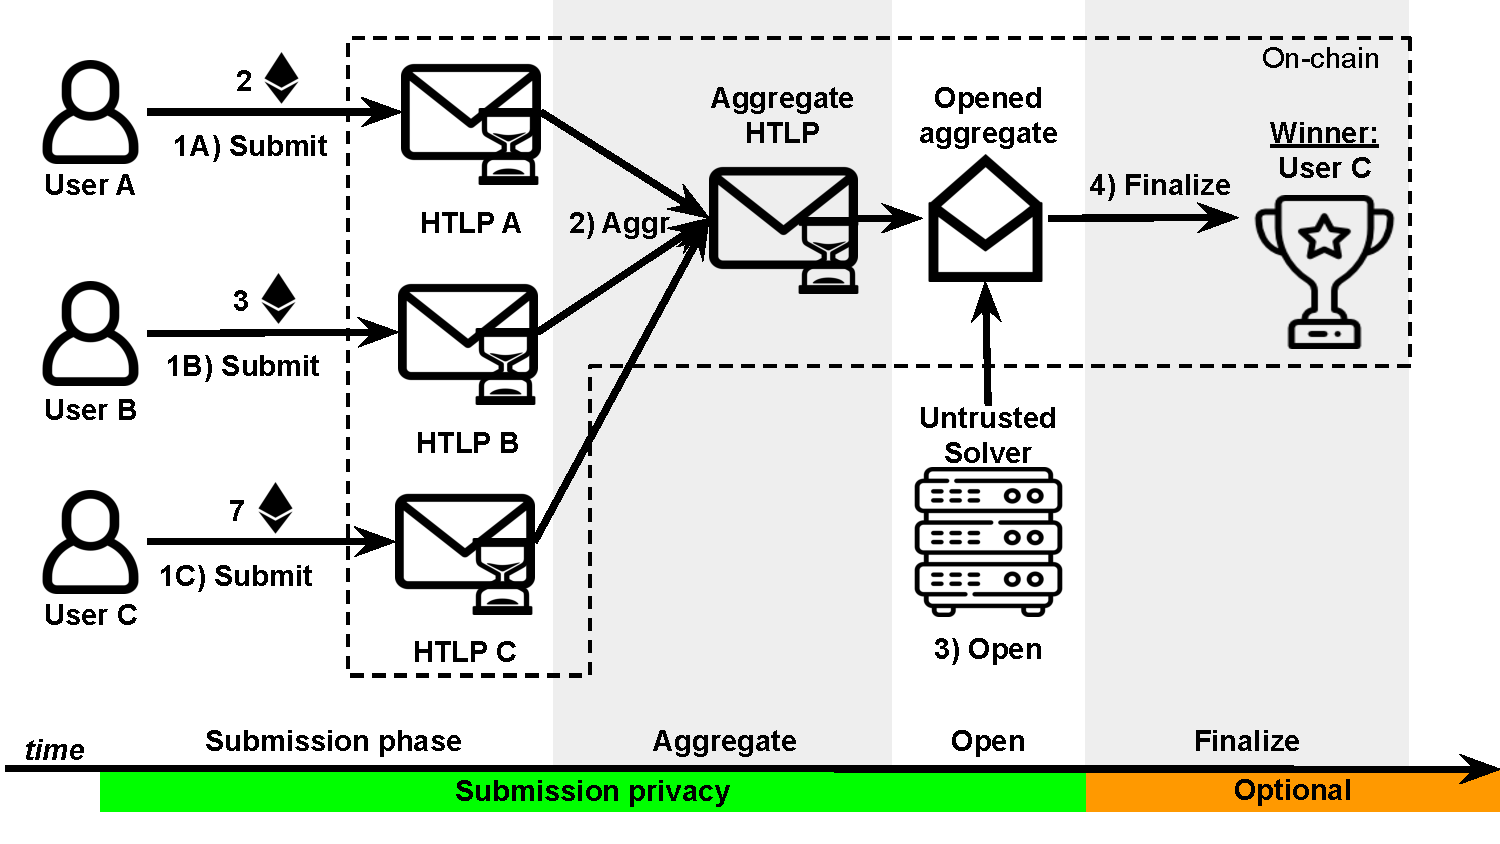
\includegraphics[width=0.95\textwidth]{cicada/figs/cicada-explainer.pdf}
    \caption{The system model of Cicada. \emph{(1) Submission phase:} users generate their bids/ballots as HTLPs and post them to a public bulletin board, e.g., a blockchain. \emph{(2) Aggregation:} an on-chain contract homomorphically combines submissions into an aggregate puzzle as they are submitted. \emph{(3) Opening:} after all submissions have been aggregated, an off-chain entity solves the aggregate HTLP using $\Ttime$ sequential steps and submits the solution to the contract. \emph{(4) Finalize:} The smart contract may do some final computation over the solution to compute the result and announces the winner. Submission privacy is ensured only until the start of the $\mathsf{Open}$ phase. 
    In \Cref{sec:everlasting_ballot_privacy}, we show how voters can pool their submissions to achieve everlasting ballot privacy.
    }
    \label{fig:cicada-explainer}
\end{figure}


We envision three types of participants, as illustrated in \Cref{fig:cicada-explainer}:
\begin{description}
    \item[Users.] We simply refer to voters or bidders as \emph{users}. Users submit bids or ballots, which we generically call \emph{submissions}. We assume some external process to establish the set of authorized users (which may be open to all).  Once users place their submissions, no further action is required of them. 
    \item[On-chain coordinator.] We refer to the tallier/auctioneer as the \emph{coordinator}, typically implemented as a smart contract that collects submissions. The coordinator transparently calculates the winner(s). In the case of an auction, they might also transfer (digital) assets to the winner(s). In an election, they might grant special privileges to the winner.%'s public key.
    \item[Off-chain solver.] We assume an untrusted \emph{solver} who unlocks the final (set of) HTLP off-chain and submits the solution(s) to the coordinator with a proof of correct opening. In principle, this could be any party, but in practice will likely be one of the parties participating in (or administering) the vote/auction or a paid marketplace~\cite{EPRINT:Abadi23,CCS:TGBKS21}.
\end{description}
\section{Voting and auction schemes}

We recall the specifics of FPTP, approval, range, and cumulative voting, along with single-item sealed bid auctions. The cryptographically relevant details of these schemes (i.e., the valid ballots' structure: their domain, Hamming weight, and norm) are summarized in~\Cref{tab:voting_schemes}. In~\Cref{sec:constructions}, we create private voting protocols for these schemes of interest.

\def\sp{\hspace{1em}}
%%------------------- BEGIN Ballot domain TABLE ----------------------
\begin{table*}[tb]
    \centering
\makebox[\linewidth]{
    \setlength{\tabcolsep}{6pt}
    \setlength{\belowbottomsep}{6pt}
    \begin{tabular}{l@{\hspace{12pt}}ccc}
        \toprule
                        & \textbf{Submission domain}    & \textbf{Hamming wt}   & \textbf{Norm} \\\midrule
        FPTP voting     & $[0,1]^m$ & $\leq 1$& $\leq 1$ \\
        Approval voting     & $[0,1]^m$ & $\leq m$& $\leq m$ \\
        Range voting  & $[0,w]^m$ & $\leq m$      & $\leq wm$ \\
        Cumulative voting  & $[0,w]^m$ & $\leq m$      & $\leq w$ \\
        Ranked-choice voting (Borda) 
                        & $\pi([0,m-1])$& $m-1$     & $m(m-1)/2$ \\
        Quadratic voting
        & $[0,\sqrt{w}]^m$& $\leq m$& $\lVert \vec{b} \rVert_2^2 = \langle \vec{b}, \vec{b} \rangle = w$ \\
        \midrule
        Single-item sealed-bid auction & $[0, w]$  & 1 & $\leq w$ \\
        % \midrule
        % Bayesian truth serum %(\Cref{sec:voting_bayesian_truth})
        %                 & $[0,1]^m \times \mathbb{N}^m$ & $1, 1$ & $1, \leq m$ \\
        \bottomrule
    \end{tabular}
}
    \caption{Requirements for the domain, Hamming weight, and norm of a vector $\vec{b}$ for it to be a valid submission in various voting/auction schemes.
    $\pi(S)$ denotes the set of permutations of $S$. The norm is an $\ell_1$ norm unless otherwise specified. $m$ is the number of candidates, and $w$ is the maximum weight that can be assigned to any candidate.
    }
    \label{tab:voting_schemes}
\end{table*}

\paragraph{Majority, approval, range, and cumulative voting.} 
In the classic first-past-the-post (FPTP) voting scheme, voters can cast a vote of $1$ (support) for one candidate and $0$ for all others. A slight generalization of FPTP is approval voting, where users can assign a $1$ vote to multiple candidates, i.e., the cast ballot $s$ can be seen as $s\in\{0,1\}^{m}$, where $m$ is the number of causes. A further generalization is range voting, where users can give each candidate up to some weight $w$ (thus, approval is the special case where $w=1$). A related scheme is cumulative voting, where users can distribute a total of $w$ votes (points) among the candidates (now FPTP is a special case where $w=1$).
In each case, each candidate's points are tallied and the candidate with the highest number is declared the winner.

\paragraph{Ranked-choice voting.} 
% In a ranked-choice voting scheme, voters can signal more fine-grained preferences among $m$ candidates. In the Borda count version~\cite{emerson2013borda}, each voter can cast $m-1$ points to their first-choice candidate, $m-2$ points to their second-choice candidate, etc. In general, they can cast $m-k$ points to their $k$\textsuperscript{th} choice. 
% Several other counting functions exist for ranked voting, but in this work, we only focus on Borda counts. Our protocols can easily be adapted to other counting functions, such as the Dowdall system~\cite{fraenkel2014borda} via minor modifications.
In a ranked-choice voting scheme, voters can signal more fine-grained preferences among $m$ candidates by listing them in order of preference. There are multiple approaches to determining the winner, including single transferrable vote (STV) and instant runoff voting (IRV). In this work, we focus on the simpler Borda count version~\cite{Emerson13}, where each voter can cast $m-1$ points to their first-choice candidate, $m-2$ points to their second-choice candidate, etc., and the candidate with the most points is the winner. Our protocols can be adapted to similar counting functions, such as the Dowdall system~\cite{FraGro14}, via minor modifications.

\paragraph{Quadratic voting.} 
In quadratic voting~\cite{LalWey18}, each user's ballot is a vector $\vec{b} = (b_1, \dots, b_m)$ such that $\langle \vec{b}, \vec{b} \rangle = \lVert \vec{b} \rVert^2_2 \leq w$. Once again, the winner is determined by summing all the ballots and determining the candidate with the most points. Thus, this is also an additive voting scheme. 
However, proving ballot well-formedness efficiently in this particular case benefits greatly from the novel application of the residue numeral system (RNS) to private voting (see~\Cref{sec:packing}).

\paragraph{Single-item sealed-bid auction.} 
In a sealed-bid auction for a single item (e.g., an NFT or domain name), users submit secret bids to the auction contract. The domain of the bids might be constrained, e.g., $b\in\{0,1\}^{k}$ (in our implementations $k\approx 8-16$; see \Cref{sec:implementation}). Therefore, bidders must prove that their bid is well-formed, i.e., falls into that domain. Once all secret bids are revealed, the contract selects the highest bidder and awards them the auctioned item. The price the winner must pay depends on the auction scheme: e.g., highest bid in a first price auction, second-highest in a Vickrey auction. %\todo{should we include this too?}\istvan{Iterated on this. Opinions?}
\subsection{Formalizing Time-Locked Voting and Auction Protocols}\label{sec:syntax}

We introduce a generic syntax for a time-locked voting/auction protocol. Any such protocol is defined for a base \emph{scoring function} $\Score: \X^n \to \Y$ (e.g., second-price auction, range voting), which takes as input $n$ submissions (bids/ballots) $s_1, \dots, s_n$ in the submission domain $\X$ and computes the election/auction result $\Score(s_1, \dots, s_n) \in \Y$. It is useful to break down the scoring function into the ``tally'' or aggregation function $\tally: \X^n \to \X'$ and the finalization function $\final: \X' \to \Y$, i.e., $\Score = \final \circ \tally$.
For example, in first-past-the-post voting, the tally function $t$ is addition, and the finalization function $f$ is $\argmax$ over the final tally/bids.
%$\Sigma : \mathcal{X}^n \rightarrow \Y$ which operates over submissions in the clear. 

% \noemi{I think the following is actually unnecessary and I'm not even sure what it was going for...} In the case of an auction, $\Y\subseteq [n]\times\mathbb{Z}^m$. Intuitively, $\Y$ provides the aggregate result of how users voted for the candidates or the number of a specific item they obtained as a result of the auction. %Although it is in theory possible to efficiently open the aggregated $\htlp$(s) given every participant's private puzzle randomness, in practice this is unrealistic. We therefore omit the optimistic opening procedure in the $\Open$ algorithm below.

\begin{definition}[Time-locked voting/auction protocol]\label{def:syntax}
A time-locked voting/auction protocol $\Pi_\Sigma = (\Setup, \Seal,\allowbreak \Aggr, \Open, \Finalize)$ is defined with respect to a base voting/auction protocol $\Sigma = \final \circ \tally$, where $\tally : \X^n \to \X'$ and $\final : \X' \to \Y$. %where $n$ is the number of participants.

\begin{description}
    \item[$\Setup(\secparam, \Ttime) \randout (\pp, \Z)$.] Given a security parameter $\secpar$ and a time parameter $\Ttime$, output public parameters $\pp$ and an initial time-locked value $\Z$.
    %HTLP that corresponds to the running tally or bid computation.
    \item[$\Seal(\pp, i, s) \randout (\Z_i, \pi_i)$.] User $i\in[n]$ seals its submission $s \in \X$ into a time-locked submission %a (list of) HTLP(s) 
    $\Z_i$. It also outputs a proof of well-formedness $\pi_i$.
    \item[$\Aggr(\pp, \Z, i, \Z_i, \pi_i) \to \Z'$.] Given a time-locked running computation %list of (tally) HTLPs 
    $\Z$, time-locked submission $\Z_i$ of user $i$, and proof $\pi_i$, the transparent contract checks the proof and potentially updates $\Z$ to $\Z'$. %aggregates the sealed submission homomorphically into $\Z$ to get an updated (tally) $\Z' = \tally(\Z, \Z_i)$.
    \item[$\Open(\pp, \Z) \to (\vec{s}, \pi_\open)$.] Open $\Z$ to $\vec{s} = \tally(s_1, \dots, s_n)$, requiring $\Ttime$ sequential steps, and compute a proof $\pi_\open$ to prove correctness of $\vec{s}$.
    \item[$\Finalize(\pp, \Z, \vec{s}, \pi_\open) \to \{y, \perp\}$.] Given proposed opening $\vec{s}$ of $\Z$ and proof $\pi_{\sf open}$, the coordinator may reject $\vec{s}$ or compute the final result $y = \final(\vec{s}) \in \Y$. %, which specifies the winner and, in the case of an auction, the amount to be paid as well as the appropriate items to be transferred.
\end{description}
\end{definition}

We note that the $\Setup(\cdot)$ algorithm in our protocols may use private randomness. In particular, our constructions use cryptographic groups (RSA and Paillier groups) that cannot be efficiently instantiated without a trusted setup (an untrusted setup would require gigantic moduli~\cite{ICICS:Sander99}). This trust can be minimized by generating the group via a distributed trusted setup, e.g.,~\cite{JACM:BonFra01,SP:CHIKMRsVW21,TCC:DamMik10}.
Alternatively, the HTLPs in our protocols could be instantiated in class groups~\cite{CCS:TCLM21}, which do not require a trusted setup; however, HTLPs in class groups are less efficient and verifying them on-chain would be prohibitively costly 
(see \Cref{sec:feasability}).

A time-locked voting/auction protocol $\Pi_\Sigma$ must satisfy the following three security properties:

\paragraph{Correctness.} 
$\Pi_\Sigma$ is \emph{correct} if, assuming setup, submission of $n$ puzzles, aggregation of all $n$ submissions, and opening are all performed honestly, $\sf Finalize$ outputs a winner consistent with the base protocol $\Sigma$.

\begin{definition}[Correctness]\label{def:correctness_cicada}
We say a voting/auction protocol $\Pi_\Sigma$ with $\Sigma: \X^n \to \mathcal{Y}$ is \emph{correct} if for all $\Ttime,\secpar \in \mathbb{N}$ and submissions $s_1, \dots, s_n \in \X$,
\[
    \Pr\left[
        \begin{aligned}
            &\\
            \Finalize &(\pp, \Z_{\sf final}, \mathcal{S}, \pi_{\sf open}) \\
            &= \Sigma(s_1, \dots, s_n)\\
            &\\
        \end{aligned}
        \middle|
        \begin{array}{c}
            (\pp, \Z) \sample \Setup(\secparam, \Ttime)~\land\\
            (\Z_i, \pi_i) \sample \Seal(\pp, i, s_i)~\forall i \in [n]~\land\\
            \Z_{\sf final} \gets \Aggr(\pp, \Z, \{i, \Z_i, \pi_i\}_{i \in [n]})~\land\\
            (\mathcal{S}, \pi_{\sf open}) \gets \Open(\pp, \Z_{\sf final}) \\
        \end{array}
    \right] = 1
\]
where the aggregation step is performed over all $n$ submissions in any order.
\end{definition}

\paragraph{Submission privacy.} 
The scheme satisfies \emph{submission privacy} if the adversary cannot distinguish between two submissions, i.e., bids or ballots. Note that this property is only ensured up to time $\Ttime$.

\begin{definition}[Submission privacy]\label{def:submission_privacy}
We say that a voting/auction protocol $\Pi_\Sigma$ with $\Sigma: \X^n \to \mathcal{Y}$ is \emph{submission private} if for all $\Ttime,\secpar \in \mathbb{N}, i \in [n]$ and all PPT adversaries $\mathcal{A}$ running in at most $\Ttime$ sequential steps, there exists a negligible function $\negl$ such that 
\begin{equation*}
    \Pr\left[
        b=b'
        \middle|
        \begin{array}{c}
            (\pp, \Z) \sample \Setup(\secparam, \Ttime)~\land\\       
            b\sample\{0,1\}~\land\\
            (\Z_i, \pi_i) \sample \Seal(\pp, i, b)~\land\\
            b'\gets\adv(\pp,\Z,i, \Z_i, \pi_i)\\
        \end{array}
    \right]
    \leq \frac{1}{2} + \mathsf{negl}(\lambda).
\end{equation*}
\end{definition}

\paragraph{Non-malleability.} 
Notice that submission privacy alone does not suffice for security: even without knowing the contents of other puzzles, an adversary could submit a value that depends on other participants' (sealed) submissions. For example, in an auction, one could be guaranteed to win by homomorphically computing an HTLP containing the sum of all the other participants' bids plus a small value $\varepsilon$. Therefore, we also require \emph{non-malleability}, which requires that no participant can take another's submission and replay it or ``maul'' it into a valid submission under its own name.

\begin{definition}[Non-malleability]\label{def:non_malleability}
We say that a voting/auction protocol $\Pi_\Sigma$ with $\Sigma: \X^n \to \mathcal{Y}$ is \emph{non-malleable} if for all $\Ttime,\secpar \in \mathbb{N}$ and all PPT adversaries $\mathcal{A}$ running in at most $\Ttime$ sequential steps, there exists a negligible function $\negl$ such that the following probability is bounded by $\negl[\secpar]$:
\begin{align*}
    \Pr\left[
        \begin{array}{c}
        \Aggr(\pp, \Z, i, \Z_i, \pi_i) \neq \Z~\land\\
        (i, \cdot, \Z_i, \pi_i) \notin \mathcal{Q}
        \end{array}
        \middle|
        \begin{array}{c}
            (\pp, \Z) \sample \Setup(\secparam, \Ttime)~\land\\
            (i, \Z_i, \pi_i) \gets \adv^{\mathcal{O}_\Seal(\pp,\cdot,\cdot)}(\pp, \Z)
        \end{array}
    \right]
    % \\
    %\leq\mathsf{negl}(\lambda)
\end{align*}
where $\mathcal{O}_\Seal(\pp, \cdot,\cdot)$ is an oracle which takes as input any $j \in [n]$ and $s_j \in \X$ and outputs $(\Z_j, \pi_j) \sample \Seal(\pp, j, s_j)$, and $\mathcal{Q}$ is the set of queries and responses $(j, s_j, \Z_j, \pi_j)$ to the oracle.
\end{definition}

\paragraph{A note on anonymity.} 
We consider user anonymity an orthogonal problem. In the applications we have in mind, users can increase their anonymity by using zero-knowledge mixers~\cite{PerSemSto19} or other privacy-enhancing overlays, e.g., zero-knowledge sets~\cite{semaphore}. Additionally, users can decouple their identities from their ballots by applying a verifiable shuffle~\cite{CCS:Neff01}, although the on-chain verification of a shuffle proof might be prohibitively costly for larger elections. 
In~\Cref{sec:everlasting_ballot_privacy} we describe how our protocols can be extended to achieve bid privacy even after the election ends, thus disclosing nothing besides a user's (non-)participation.

%\todo{can use (verifiable) shuffling/Semaphore or compose with something like TornadoVote~\cite{tornadovote} to anonymize voters/bidders. Refer to \cref{sec:everlasting_ballot_privacy}}
\section{The Cicada Framework}\label{sec:cicada_framework}

We present Cicada, our framework for non-interactive private auctions/elections, in \Cref{fig:cicada}. Cicada can be applied to voting and auction schemes where the scoring function $\Score = f \circ t$ has a linear tally function $t$. The framework uses a linear HTLP (\Cref{sec:tlp}), vector packing scheme (\Cref{sec:packing}), and matching NIZK (\Cref{sec:sigmas}) to ensure correctness of submissions by proving both the well-formedness of the puzzle and the solution's membership in $\X$.

At a high level, Cicada enables auction or voting schemes with the following five steps. 
\emph{First}, system participants agree on a delay parameter $\Ttime$ and packing parameter $\ell$. The $\Setup$ algorithm outputs HTLP public parameters $\pparam$ (note this might require private randomness) and initializes a set of the tally HTLPs $\mathcal{Z}$ containing zeros. 
\emph{Second}, a user $i$ uses the $\Seal$ algorithm to encode their submission (a bid or ballot) $\vec{v}_i$ into (a set of) HTLP(s) $\Z_i$. $\Seal$ also outputs a NIZK $\pi_i$ proving that the submission $\Z_i$ is well-formed, i.e., is in the domain $\mathcal{X}$ of the scoring function $\Score$. Users will send these submissions and corresponding proofs to the on-chain coordinator. 
\emph{Third}, the coordinator (Cicada smart contract) runs $\Aggr$ to verify the user-submitted proof $\pi_i$, and if it is valid, aggregate the user submission $\Z_i$ into the tally HTLPs $\Z$, resulting in updated tally HTLP(s) $\Z'$. 
\emph{Fourth}, after the voting/bidding period has ended, any party can open the tally HTLPs $\Z$ off-chain by running $\Open$, which outputs the opening(s) $\mathcal{S}$ of the tally HTLP(s) $\Z$ along with a proof of correct opening $\pi_{\textsf{open}}$ (using a proof of solution $\pos$, see \Cref{sec:sigmas}). The off-chain solver will send $\mathcal{S}, \pi_{\mathsf{open}}$ to the contract. 
\emph{Fifth}, the on-chain contract runs $\Finalize$ to verify the correctness of $\mathcal{S}$ by checking $\pi_{\mathsf{open}}$. If the check passes, it computes the auction/election winner(s) as $y=f(\vec{v})$.

% \noemi{In Cicada we need to talk about the function that is applied to the final tally, not the ballots -- maybe we could introduce a definition of ``linear'' protocols $\Sigma : \X^n \to \Y$ which are those functions that have an associated function $\Sigma_{\sf winner}: \X' \to \Y$ such that $\Sigma_{\sf winner}(t) = \Sigma(s_1, \dots, s_n)$ where $t = f(s_1, \dots, s_n)$ for some linear function $f$.}
%\noemi{difference between $\Sigma$ and $\Sigma_{\sf winner}$ is the domain, $\X^n$ and $\X$, resp.}

Intuitively, submission privacy follows from the security of the HTLP and zero-knowledge of the NIZK used: the submission can't be opened before time $\Ttime$ and none of the proofs leak any information about it. Non-malleability is enforced by requiring the NIZK to be a proof of knowledge and including the user's identity $i$ in the instance to prove, e.g., including it in the hash input of the Fiat-Shamir transform. This prevents a malicious actor from replaying a different user's ballot correctness proof.
% \istvan{Correctness is due to the correctness of the underlying NIZKs. Submission privacy is reduced to the HTLP sequentiality, while non-malleability is ensured by the proof of knowledge property of our applied NIZKs.} 

\begin{figure*}[t!]
\begin{mdframed}
\begin{center}
    \textbf{The Cicada Framework}
\end{center}
Let $\Sigma: \X^n \rightarrow \Y$ be the scoring function of a voting/auction scheme
where $\Score = f \circ t$ for a linear function $t$ and
% $\Sigma = f \circ g$ for some linear function $g$ and 
$\X = [0,w]^m$. 
Let $\htlp$ a linear HTLP, $\Ttime \in \NN$ a time parameter representing the election/auction length, and $(\PSetup, \pack, \unpack)$ a packing scheme.
Let $\NIZK$ be a NIZKPoK for 
submission correctness (language depends on $\Sigma, \htlp$; see \Cref{sec:sigmas})
% the language $\{(i, Z) : \exists x \text{ s.t. } Z \in {\sf Im}(\htlp.{\sf Gen}(\pack(x))) \land\ x \in \X\}$ 
and \pos\ be a proof of correct HTLP solution (see \Cref{sec:sigmas}). 

\hrulefill %%%%%%%%%%%%%%%%%%%%%%%%%%%%%%
\begin{description}
    \item[$\Setup(\secparam, \Ttime, \ell) \randout (\pp, \Z)$.] 
    Set up the public parameters $\pp_{\NIZK} \sample \NIZK.\Setup(\secparam)$, $\pp_{\sf tlp} \sample \htlp.\Setup(\secparam, \Ttime)$, and $\pp_{\sf pack} \gets \PSetup(\ell, w)$. 
    Let $\Z = \{Z_j\}_{j \in [m/\ell]}$ where $Z_j \sample \htlp.{\sf Gen}(0)$. Output $\pp := (\pp_{\sf tlp}, \pp_{\sf pack}, \pp_\NIZK)$ and $\Z$.
    \item[$\Seal(\pp,i, \vec{v}_i) \randout (\Z_i, \pi_i)$.] Parse $\vec{v}_i := \vec{v}_{i,1} || \dots || \vec{v}_{i,m/\ell}$. Compute $Z_{i,j} \gets \htlp.{\sf Gen}(\pack(\vec{v}_{i,j}))~\forall j \in [m/\ell]$ and $\pi_i \gets \NIZK.\prove((i, \Z_i), \vec{v}_i)$.
    % $s_{i,j} \gets \pack(\vec{v}_{i,j})$ for all $j \in [m/\ell]$. 
    Output $(\Z_i := \{Z_{i,j}\}_{j \in [m/\ell]}, \pi_i)$ 
    \item[$\Aggr(\pp,\Z,i,\Z_i,\pi_i) \rightarrow \Z'$.] If $\NIZK.\vrfy((i, \Z_i), \pi_i) = 1$, update $\Z$ to $\Z \boxplus \Z_i$. %, where $\boxplus$ is applied pairwise to elements of $\Z,\Z_i$.
    \item[$\Open(\pp,\Z) \rightarrow (\mathcal{S}, \pi_{\sf open})$.] Parse $\Z := \{Z_j\}_{j \in [m/\ell]}$ and solve for the encoded tally $\mathcal{S} = \{s_j\}_{j \in [m/\ell]}$ where $s_j \gets \htlp.{\sf Solve}(Z_j)$. Prove the correctness of the solution(s) as $\pi_{\sf open} \gets \pos.{\sf Prove}(\mathcal{S}, \Z, 2^\Ttime)$ and output $(\mathcal{S}, \pi_{\sf open})$.
    \item[$\Finalize(\pp, \Z, \mathcal{S}, \pi_{\sf open}) \rightarrow \{y,\perp\}$.] If $\pos.{\sf Verify}(\mathcal{S}, \Z, 2^\Ttime, \pi_{\sf open}) \neq 1$, return $\perp$. Otherwise, parse $S := \{s_j\}_{j \in [m/\ell]}$ and let $\Vec{v} := \vec{v}_1 || \dots || \vec{v}_{m/\ell}$, where $\vec{v}_j \gets \unpack(s_j)~\forall j \in [m/\ell]$. Output 
    % $y = f(\vec{v})$.
    $y$ such that $y = \Sigma(\vec{v})$.
\end{description}
\end{mdframed}
\caption{The Cicada framework for non-interactive private auctions and elections.}
\label{fig:cicada}
\end{figure*}

As we will see next, this captures many common schemes such as cumulative voting and sealed-bid auctions. 
Cicada introduces a crucial design choice via the packing parameter $\ell\in[m]$, which defines a storage-computation trade-off that we detail in~\Cref{sec:implementation}. %The on-chain footprint of a protocol is minimized by using a ballot correctness proof system $\sf NIZK$ with low verification cost. % this seems kind of obvious? And if anything it belongs in the implementation section

% \section{Application to voting schemes}\label{sec:voting}

% \todo{revisit this} The main reason we are interested in building protocols for cardinal voting schemes is that they allow voters to express more fine-grained preferences. Put differently, they bypass Arrow's impossibility theorem~\cite{arrow1950difficulty}, i.e., cardinal voting schemes satisfy non-dictatorship, unrestricted domain, independence of irrelevant alternatives and Pareto efficient. 

\paragraph{Additive voting.}
Many common voting schemes are ``additive'', meaning each ballot (a length-$m$ vector) is simply added to the tally, and a finalization function $f$ is applied to the tally after the voting phase has ended to determine the winner. 
Additive voting schemes include first-past-the-post (FPTP), approval, range, and cumulative voting. Simple ranked-choice voting schemes, e.g., Borda count~\cite{Emerson13}, are also additive, differing only in what qualifies as a ``proper'' ballot (restrictions on vector entry domain, vector norm, etc.; see \Cref{tab:voting_schemes}). 
Thus, we can use Cicada to instantiate private voting protocols for all these schemes.

% \paragraph{Majority vote and approval voting.}
% We start off by describing a protocol for approval voting. Approval voting is a generalization of majority vote, whereby, a voter can cast a vote for multiple candidates. In case of a majority vote, a ballot can be thought of as a binary vector of Hamming weight $1$, while approval voting lifts this restriction, i.e., the ballot can be any length-$m$ binary vector $\vec{b} \in\{0,1\}^{m}$. The challenge is to design a protocol that applies a single HTLP for tallying the approval votes.

% Following~\cite{hirt2000efficient}, we encode the $i$th voter's ballot as the integer
% \begin{equation}\label{eq:approval_voting_ballot_encoding}
%     % b_j\in \Big\{
%     % \sum\limits_{i=1}^{m} b_j^{(i)} (n+1)^{i-1}: b_j^{(i)} = 1 \iff\textit{j votes for candidate i}\in[m]\Big\}. 
%     b_i\in \Big\{
%     \sum\limits_{j=1}^{m} b_i^{(j)} (n+1)^{j-1}: b_i^{(j)} = 1 \iff\textit{i votes for candidate j}\in[m]\Big\}. 
% \end{equation}
% Note the number of votes for candidate $j$ can be obtained as $\sum\limits^{n}_{i=1}b_i\bmod{(n+1)^{j-1}}$.

% \begin{figure}[h!]
% \begin{mdframed}
% \begin{description}
%     \item[$\mathsf{Setup}(\secparam, \Ttime) \randout (\pparam, Z^*)$.]  Set up HTLP parameters $\pparam_{\sf tlp} \sample \htlp.\Setup(\secparam, \Ttime)$. Let $Z^* \sample \htlp.{\sf Gen}(\pparam_{\sf tlp}, 0)$. Output $\pparam := (\pparam_{\sf tlp},Z^*)$.
%     \item[$\Seal(\pparam,i,b_i) \randout (Z_i, \pi_{\sf i})$.] Let $b_i$ encode the $i$th user's approval vote as in Equation~\ref{eq:approval_voting_ballot_encoding}. Let $Z_i \gets \htlp.{\sf Gen}(\pparam_{\sf tlp}, b_i)$. The  correctness proof $\pi_i$ is obtained as $\pi_i:=\bigwedge\limits_{i=1}^{m}\zkprove(\mathcal{R}_{\pokemon}(Z_i/Z'_j,0,n^{j-1};b_i) \lor\mathcal{R}_{\pokemon}(Z_i/Z'_j,1,n^{j-1};b_i))$, where $Z'_j$ is the residual approval vote, i.e., $Z'_j\gets\htlp.{\sf Gen}(\pparam_{\sf tlp}, b_i\mod{n^{j-1}})$. 
    
%     Output $(Z_i,\pi_i)$.
%     \item[$\Aggr(\pparam,Z^*,Z_j,\pi_{\sf j}) \rightarrow Z^*$.] If $\zkvfy((\pparam,j,Z_j),\pi_{\sf j}) \neq 1$, leave $Z^*$ unchanged and abort. Otherwise, update $Z^* = Z^* \oplus Z_j$.
%     \item[$\Open(\pparam,Z^*,\mathcal{R}) \rightarrow s^*$.] Solve the tally puzzle for $s^* \gets \htlp.{\sf Solve}(\pparam_{\sf tlp}, Z^*)$.
%     \item[$\Finalize(\pparam, s^*) \rightarrow {\sf winner}$.] Compute the sum of the votes for each candidate $j \in [m]$ as $s^*_j := s^* \mod{n^{j-1}}$. The winner is $\argmax_j \{s^*_1, \dots, s^*_m\}$.
% \end{description}


% \end{mdframed}
% \caption{A protocol for approval voting among $m$ candidates using a single HTLP.}
% \label{fig:voting_approval}
% \end{figure}

% \paragraph{Ranked choice voting, range voting, and cumulative voting.}

% In a na\"ive Borda count protocol, the tally consists of $m$ HTLPs $\{Z^{*}_i\}^{m}_{i=1}$ (one per candidate) that encode the accumulated points of each candidate, initially set to $0$.  During the voting phase, each voter creates $m$ HTLPs $\{Z_i\}^{m}_{i=1}$ encoding integers from $0$ to $m-1$. Afterwards, voters homomorphically add each ballot HTLP $Z_i$ to the corresponding tally HTLP $Z^{*}_i$. This solution is suboptimal in terms of the number of HTLPs needed. 
% 
% We show a protocol that requires only a single HTLP. Let the $i$th voter's preference vector be defined as $\mathbf{q^{(i)}}=(q^{(i)}_1,q^{(i)}_2,\dots,q^{(i)}_m)$, which is required to be a permutation of $[0,m-1]$ .
% % $\forall j:q^{(i)}_j\in[0,m-1]\land\forall j,k: q^{(i)}_{j}\neq q^{(i)}_k$ i.e., it is a permutation of $[0,m-1]$. 
% % Let $\mathbf{p}=(p_1,p_2,\dots,p_m)$ be a vector of prime numbers such that $\min_{i}p_i\geq (m-1)n$ and $\prod\limits_{i=1}^{m} p_i\leq N$.
% Now encode $\vec{q}^{(i)}$ as an integer $s_i$ using the Chinese Remainder Theorem (see \cref{sec:packing}) and encode it in an HTLP $Z_i$.
% % Specifically, $s_i\equiv q^{(i)}_{j}\mod{p_j}$, which can be efficiently found by the Chinese Remainder's Theorem (CRT).
% The user submits their puzzle $Z_i$ with the accompanying zero-knowledge proofs for ballot correctness, and the on-chain contract homomorphically adds $Z_i$ and $Z^*$.

% At the end of the voting phase, a single party solves the tally HTLP $Z^*$ to obtain the solution $s^{*}$. We claim that the total preference points (Borda counts) for candidate $j$ can be computed as $s^{*}\mod{p_j}$. The correctness of this protocol for ranked voting follows from the observation that for any preference $j$, we have 
% \begin{equation}\label{eq:borda_correctness_argument}
%     s^{*}\bmod{p_j}=\sum\limits^n_{i=1}s_i\bmod{p_j}\equiv\sum\limits^n_{i=1}q^{(i)}_j\bmod{p_j}=\sum\limits^n_{i=1}q^{(i)}_j\leq(m-1)n. 
% \end{equation}

\begin{theorem}\label{thm:cicada}
    Given a linear scoring function $\Sigma$, a secure NIZKPoK $\NIZK$ and proof of solution $\pos$, a secure $\htlp$, and a packing scheme $({\sf PSetup},\allowbreak \pack,\allowbreak \unpack)$, the Cicada protocol $\Pi_\Sigma$ (\Cref{fig:cicada}) is a secure time-locked voting/auction protocol. % i.e., it satisfies correctness, bid/ballot privacy, and non-malleability.
\end{theorem}

% We delegate the full proof to \Cref{sec:secproofs}.
\begin{proof}
\def\Exp{\ensuremath{\mathsf{ExpSPriv}_{\Pi_\Sigma}^\adv(\secpar,\Ttime,i)}}
    For simplicity, we give a proof for the simple case of $\X=[0,1]$, i.e., submissions consist of a single bit, but our argument generalizes to larger domains $\X$. Let $n \in \mathbb{N}$ be the number of users.

    The correctness of the Cicada framework (cf.~\Cref{def:correctness_cicada}) follows by construction and from the correctness of the underlying building blocks (i.e., soundness in the case of the proof systems).
    
    Next, we prove submission privacy.
    Let $\Exp$ be the original submission privacy game for the Cicada scheme $\Pi_\Sigma$ with $\Ttime$-bounded adversary $\adv$, cf.~\Cref{def:submission_privacy}. We define a series of hybrids to show that 
    \[ 
        \Pr[\Exp = 1] \leq \negl 
    \]
    for all $\secpar,\Ttime \in \mathbb{N}$ and $i\in[n]$.
    
    \underline{$\hybrid_0$:} This is the original game $\Exp$, where $Z_i \gets \htlp.{\sf Gen}(b)$ and $\pi_i \gets \NIZK.\prove(i, Z_i, b)$.
    
    \underline{$\hybrid_1$:} Replace $\pi$ with $\tilde{\pi} \gets {\sf NIZK}.\Sim(i, Z_i)$. $\hybrid_1$ is indistinguishable from $\hybrid_0$ by the zero-knowledge property of $\sf NIZK$.

    \underline{$\hybrid_2$:} Replace $Z_i$ with $Y_i \gets \htlp.{\sf Gen}(1-b)$ and $\tilde{\pi}$ with $\tilde{\sigma} \gets {\sf NIZK}.\Sim(i, Y_i)$. $\hybrid_1$ and $\hybrid_2$ are indistinguishable because the distributions $\{Z_i, \Sim(i, Z_i)\}$ and $\{Y_i, \Sim(i, Y_i)\}$ are indistinguishable since $\{Z_i\}, \{Y_i\}$ are indistinguishable by the security of $\htlp$.

    % \underline{$\hybrid_3$:} Replace $\tilde{\pi}$ with $\tilde{\sigma} \gets {\sf NIZK}.\Sim(i, Y_i)$. $\hybrid_3$ is indistinguishable from $\hybrid_2$ again by security of $\htlp$: since the distributions of $Z_i, Y_i$ are indistinguishable, so must the distributions ...
    
    \underline{$\hybrid_3$:} Replace $\tilde{\sigma}$ with $\sigma \gets \NIZK.\prove(i, Y_i, 1-b)$. $\hybrid_3$ is indistinguishable from $\hybrid_2$ by the zero-knowledge property of $\sf NIZK$.

    This series of hybrids implies $\Pr[b'=b] \approx_\secpar \Pr[b'=1-b]$, where $b'$ is the output of $\adv$ in $\hybrid_0$ or $\hybrid_3$, respectively. Therefore $\Pr[\Exp = 1] \leq \frac{1}{2} + \negl[\secpar]$.
    
    % --- reduction attempt ---
    % Suppose towards a contradiction that there exists a $\Ttime$-bounded adversary $\adv$ who wins the submission privacy game with non-negligible probability. We will use give a $\Ttime$-bounded adversary $\bdv$ capable of violating either the zero-knowledge of $\sf NIZK$ or the privacy of $\htlp$.

    % Given a puzzle $Z$ containing an unknown bit $b_1$ and a proof $\pi$ that some independent unknown bit $b_2 \in [0,1]$, $\bdv$ constructs two different queries $(Z, \tilde{\pi})$ and $(\tilde{Z}, \pi)$ as follows: sample $i \sample [n]$ and compute $\tilde{\pi} \gets {\sf NIZK}.\Sim(i, Z)$ and $\tilde{Z} \gets \htlp.{\sf Gen}(0)$. Query $\adv$ on both 

    Finally, we show that if $\NIZK$ is a PoK and $\htlp$ is secure, then Cicada is non-malleable, cf.~\Cref{def:non_malleability}. Suppose towards a contradiction that Cicada is malleable. We will use this and the fact that $\NIZK$ is a PoK to construct an adversary $\bdv$ which has non-negligible advantage in the $\htlp$ security game. Again, we work in the simple case $\X = [0,1]$, i.e., $m,\ell,w=1$, but the argument generalizes to other parameter settings.
    
    Since by our assumption Cicada is malleable, there exists $\adv$ which outputs $(i, \cdot, \Z_i, \pi_i) \notin \mathcal{Q}$ such that $\NIZK.\vrfy((i,\allowbreak \Z_i), \pi)=1$ with non-negligible probability. 
    % Also, $\sf NIZK$ is a PoK, so it has an efficient knowledge extractor $\Ext$. 
    Given a puzzle $Z_b$ containing some unknown bit $b$, $\bdv$ works as follows. First, it computes $(\pparam, Z) \sample \Setup(\secparam, \Ttime, 1)$ and sends them to the non-malleability adversary $\adv$. $\bdv$ responds to $\adv$'s oracle queries $(j, b_j)$ with honestly computed $(Z_j, \pi_j)$, keeping track of queries and responses in the set $\mathcal{Q}$. When $\adv$ outputs $(i, Z_i, \pi_i)$, $\bdv$ looks for $(i, b_i, Z_i, \pi_i) \in \mathcal{Q}$ and outputs $b_i$. Since $\adv$ has non-negligible advantage, it follows that $\NIZK.\vrfy((i, Z_i), \pi_i) = 1$. This implies that either $\Pr[b_i=b] = \frac{1}{2} + \negl[\secpar]$ or $\NIZK$ is not knowledge sound. Both possibilities contradict our assumptions, namely that the $\htlp$ is secure and the $\NIZK$ is knowledge sound. Thus, Cicada must be non-malleable.
\end{proof}
\subsection{Ballot/Bid Correctness Proofs}\label{sec:sigmas}

For our NIZKs, we assume HTLPs are of the form $(u,v) = (g^r, h^r y^s) \in \GG_1 \times \GG_2$, where $\GG_1, \GG_2$ are groups of unknown order. 
This captures all known constructions of HTLPs: in the case of the Paillier HTLP (\Cref{con:paillierHTLP}), $\GG_1 = \mathbb{J}_N$, $\GG_2 = \ZZ_{N^2}^*$, $h = (g^{2^\timeT})^N$, and $y = 1+N$. For the exponential ElGamal HTLP (\Cref{con:exp_elgamalHTLP}), $\GG_1 = \GG_2 = \ZZ_N^*$, $h = g^{2^\timeT}$, and $y \in \GG_1$. And for the class group HTLP~\cite{CCS:TCLM21}, $\GG_1,\GG_2$ are cyclic subgroups of the respective class groups $Cl(\Delta_K), Cl(q^2\Delta_K)$, respectively, $h = \psi_q(G^{2^\timeT})$ where $G$ is a generator of $\GG_1$ and $\psi_q : Cl(\Delta_K) \to Cl(q^2 \Delta_K)$ is an injective map, and $y \in \GG_2$ is the generator of a subgroup in which the discrete logarithm problem is easy (see \cite{CCS:TCLM21} for details).
% \noemi{what about HTLP from class groups?} % see this paper https://inria.hal.science/hal-03466495/document % diff link https://eprint.iacr.org/2021/1272

\paragraph{Proof of solution}

% The discrete logarithm proof can be instantiated with the classic sigma protocol by Schnorr~\cite{CRYPTO:Schnorr89} in a group of unknown order, where the challenge should be a prime (see \Cref{sec:nizks}):

% % \begin{figure}[h]
    % \centering
    \begin{mdframed}
    \begin{center}
        \textbf{Zero-knowledge proof of knowledge of discrete logarithm (\podlog)}
    \end{center}
    \hfill\\
    \textbf{Public parameters:} Group of unknown order $\GG$ with generator $g$. \hfill\\
    \textbf{Public input:} $u,w \in gp$. \hfill\\
    \textbf{Private input:} $x \in \ZZ$ such that $w = u^x$.
    \begin{enumerate}
        \item $\mathcal{P}$ samples $\alpha \sample \ZZ$ and sends $A := u^\alpha$.
        \item $\mathcal{V}$ sends a challenge $e \sample \mathsf{Primes}(\secpar)$.
        \item $\mathcal{P}$ computes $z = x e + \alpha$,
        which it sends to $\mathcal{V}$.
    \end{enumerate}
    $\mathcal{V}$ accepts iff $u^e A = w$.
    \end{mdframed}
%     \label{fig:zkpokdlog}
% \end{figure}

During the finalization phase of our protocol, any party can solve the final HTLP off-chain and submit a solution to the contract. To enforce the correctness of this solution we require the solver to include a proof of the following relation:
\begin{equation}
    \mathcal{R}_{\pos}=\{((y,u,v,w\in\mathbb{G},s\in\mathbb{Z});\bot): w = u^{2^\timeT} \land\ v = w y^s \in \GG\}
\end{equation}

We call such a proof system $\pos = (\mathsf{Prove}, \mathsf{Verify})$. It can be realized as the conjunction of two proofs of exponentiation ($\poe$)~\cite{ITCS:Pietrzak19b,EC:Wesolowski19} for $w = u^{2^T}$ and $y^s = v/w$.
A \poe\ is a proof for the following relation:
\[
    \mathcal{R}_{\poe}=\{((u,w\in\mathbb{G},x\in\mathbb{Z});\bot):w=u^{x}\in\mathbb{G}\}
\]

Note that there is no witness in the $\mathcal{R}_{\poe}$ relation, i.e., the verifier knows the exponent $x$. The primary goal of the \poe\ proof system for the verifier is to outsource a possibly large exponentiation in a group $\mathbb{G}$ of unknown order.

\begin{mdframed}
\begin{center}
        \textbf{Wesolowski's proof of exponentiation  protocol (\poe)}
    \end{center}
\hfill\\    
\textbf{Public parameters:} $\mathbb{G}\sample\mathit{GGen}(\lambda)$.\hfill\\
\textbf{Public inputs:} $u,w\in\mathbb{G},x\in\mathbb{Z}$.\hfill\\
\textbf{Claim:} $u^x=w$.
\begin{enumerate}
    \item $\mathcal{V}$ sends $l\sample\mathsf{Primes}(\lambda)$ to $\mathcal{P}$.
    \item $\mathcal{P}$ computes $q=\lfloor\frac{x}{l}\rfloor\in\mathbb{Z}\land r\in[l]$, where $x=ql+r$. $\mathcal{P}$ sends $Q=u^q\in\mathbb{G}$ to $\mathcal{V}$.
    \item $\mathcal{V}$ computes $r=x\bmod{l}$.
\end{enumerate}
    $\mathcal{V}$ accepts iff $w=Q^{l}u^{r}$.
\end{mdframed}

Observe that the verifier sends a prime number as a challenge. When we make this protocol non-interactive via the Fiat-Shamir transform, we use a standard $\textsf{HashToPrime}(\cdot)$ function to generate the correct challenge for the prover. In our implementation, we use the Baillie-PSW primality test~\cite{PomSelWag80} to show that a randomly hashed challenge is indeed prime. 

\paragraph{Proofs of well-formedness}

To prove that HTLP ballots are well-formed during the submission phase, we will use several different proofs of knowledge about TLP solutions. 
Most of our protocols make use of the fact that for such HTLPs, $v$ has the same structure as a Pedersen commitment~\cite{C:Pedersen91}.

% \footnote{To be precise, one must actually use $\ZZ_N^* / \{\pm 1\}$ to remove any non-identity elements of known order (namely $-1$).}

Since we are operating in groups of unknown order, to circumvent the impossibility result of \cite{TCC:BanCamKre10} and achieve negligible soundness error for Schnorr-style sigma protocols, we assume access to some public element(s) of $\GG_1, \GG_2$ whose representations are unknown. We prove security assuming $\GG_1, \GG_2$ are generic groups output by some randomized algorithm $GGen(\secpar)$.
% Due to this change, the verifier's challenges must also be sampled from the set of $\secpar$-bit primes, denoted ${\sf Primes}(\secpar)$. \noemi{Actually, this is specific to Wesolowski and other \emph{efficient} dlog proofs in groups of unknown order, e.g. \poke.}
For more on instantiating Schnorr-style protocols in groups of unknown order while maintaining negligible soundness error, see \cite{C:BonBunFis19}.

\paragraph{Well-formedness and knowledge of solution} 
To prove knowledge of a puzzle solution in zero-knowledge, our starting point is the folklore Schnorr-style protocol for knowledge of a Pedersen-committed value. Our protocol \zkpoks is shown below.

% \begin{figure}[h]
    % \centering
    \begin{mdframed}
    \begin{center}
        \textbf{zkPoK of TLP solution (\zkpoks)}
    \end{center}
    \hfill\\
    \textbf{Public parameters:} $\GG_1, \GG_2 \sample GGen(\secpar)$, $b > 2^{2\secpar}\sizeof{\GG_i}~\forall i \in \{1,2\}$, and $g \in \GG_1, h,y \in \GG_2$. \hfill\\
    \textbf{Public input:} HTLP $Z = (u,v)$. \hfill\\
    \textbf{Private input:} $s, r \in \ZZ$ such that $Z = (g^r, h^r y^s)$.
    \begin{enumerate}
        \item $\mathcal{P}$ samples $\alpha, \beta \sample [-b,b]$ and sends $A := h^\alpha y^\beta, B := g^\alpha$ to $\mathcal{V}$.
        \item $\mathcal{V}$ sends a challenge $e \sample [2^\secpar]$. %$e \sample \mathsf{Primes}(\secpar)$.
        \item $\mathcal{P}$ computes $w = r e + \alpha$ and $x = s e + \beta$,
        which it sends to $\mathcal{V}$.
    \end{enumerate}
    $\mathcal{V}$ accepts iff the following hold:
    \begin{align*}
        v^e A = h^w y^x \\
        u^e B = g^w
    \end{align*}
    \end{mdframed}
%     \label{fig:zkpoks}
% \end{figure}
 
\paragraph{Equality of solutions} 
Again, our starting point is the folklore protocol of equality of Pedersen-committed values: given two HTLPs with second terms $v_1, v_2$, if the solutions are equal the quotient is $v_1/v_2 = h^{r_1-r_2}$. To prove the equality of the solutions, it therefore suffices to show knowledge of the discrete logarithm of $v_1/v_2$ with respect to $h$ using Schnorr's classic sigma protocol~\cite{C:Schnorr89} with the previously described adjustments. Because of its simplicity we do not explicitly write out the protocol, which we will refer to as \zkposeq.

% % \begin{figure}[h]
    % \centering
    \begin{mdframed}
    \begin{center}
        \textbf{Zero-knowledge proof of equality of TLP solutions (\zkposeq)}
    \end{center}
    \hfill\\
    \textbf{Public parameters:} Semiprime $N$ and $h, y \sample \ZZ_N^*$. \hfill\\
    \textbf{Public input:} Exponential ElGamal TLPs $Z_1 = (u_1, v_1), Z_2 = (u_2, v_2)$ (\Cref{con:exp_elgamalHTLP}).\hfill\\
    \textbf{Private input:} $s, r_1, r_2 \in \ZZ_N$ such that $v_1 = h^{r_1} y^s$ and $v_2 = h^{r_2} y^s$. (We will prove this by proving knowledge of the discrete log of $v_1/v_2$ wrt $h$.)
    \begin{enumerate}
        \item $\mathcal{P}$ samples $\alpha \sample \ZZ_N$ and sends $A := h^\alpha$.
        \item $\mathcal{V}$ sends a challenge $e \sample \mathsf{Primes}(\secpar)$.
        \item $\mathcal{P}$ computes $x = (r_1 - r_2) e + \alpha$,
        which it sends to $\mathcal{V}$.
    \end{enumerate}
    $\mathcal{V}$ accepts iff $(v_1/v_2)^e A = h^x$.
    \end{mdframed}
%     \label{fig:zkpokseq}
% \end{figure}
\noemi{This should generalize to the Paillier-based HTLP too}

%-----------------------------------------------------  BEGIN zkPoKSEq **** OLD **** --------------------------------------------------------------
% \begin{figure}[h]
%     \centering
    % \begin{mdframed}
    % \begin{center}
    %     \textbf{Proof of Equality of TLP solutions (\zkposeq)}
    % \end{center}
    % \hfill\\
    % \textbf{Public parameters:} Semiprime $N$ and $h, y \sample \ZZ_N^*$. \hfill\\
    % \textbf{Public input:} Exponential ElGamal TLPs $Z_1 = (u_1, v_1), Z_2 = (u_2, v_2)$.\hfill\\
    % \textbf{Private input:} $s, r_1, r_2 \in \ZZ_N$ such that $v_1 = h^{r_1} y^s$ and $v_2 = h^{r_2} y^s$. %(We will prove this by proving knowledge of the solutions of $v_1$ and $v_2$ as well as knowledge of the discrete log of $v_1/v_2$ wrt $h$.)
    % \begin{enumerate}
    %     \item $\mathcal{P}$ samples $\alpha_1, \alpha_2, \beta \sample \ZZ_N$ and sends $A_1 := h^{\alpha_1} y^{\beta}, A_2 := h^{\alpha_2} y^{\beta}$ to $\mathcal{V}$.
    %     \item $\mathcal{V}$ sends a challenge $e \sample \mathsf{Primes}(\secpar)$.
    %     \item $\mathcal{P}$ computes $w_1 = \alpha_1 + e r_1$, $w_2 = \alpha_2 + e r_2$, and $x = \beta + e s$,
    %     which it sends to $\mathcal{V}$.
    % \end{enumerate}
    % $\mathcal{V}$ accepts iff the following hold:
    % \begin{align*}
    %     Z_1^e A_1 = h^{w_1} y^{x} \\
    %     Z_2^e A_2 = h^{w_2} y^{x}
    % \end{align*}
    % \end{mdframed}
%     \caption{Zero-knowledge proof of equality of two TLP solutions.}
%     \label{fig:zkposeq}
% \end{figure}

\paragraph{Binary solution} 
In an FPTP vote for $m=2$ candidates, users only need to prove that their ballot $(g^r,h^ry^s)$ encodes $0$ or $1$. More formally, users prove the statement $(u=g^r\land v=h^r)\lor(u=g^r\land vy^{-1}=h^r)$. This can be proved using the OR-composition~\cite{C:CraDamSch94} of two discrete logarithm equality proofs~\cite{C:ChaPed92} with respect to bases $g$ and $h$ and discrete logarithm $r$. A similar proof strategy could be applied if the user has multiple binary choices, e.g., approval and range voting. The OR-composition of multiple discrete logarithm equality proofs yields a secure ballot correctness proof for those voting schemes. 

\paragraph{Positive solution} 
We use Groth's trick~\cite{ACNS:Groth05}, based on the classical Legendre three-square theorem from number theory, to show that a puzzle solution $s$ is positive by showing that $4s+1$ can be written as the sum of three squares. Our protocol deals only with the second component of the TLP, making use of the proof of solution equality (\zkposeq) described above and a proof that a TLP solution is the square of another (\zkposqs, described next).

% \begin{figure}
%     \centering
    \begin{mdframed}
    \begin{center}
        \textbf{Proof of positive solution (\zkpopos)}
    \end{center}
    \hfill\\
    \textbf{Public parameters:} $\GG_2 \sample GGen(\secpar)$, a secure $\htlp$, and $h,y \in \GG_2$. \hfill\\
    \textbf{Public input:} $v \in \GG_2$ such that $(\cdot,v) \in {\sf Im}(\htlp.{\sf Gen})$. \hfill\\
    \textbf{Private input:} $s, r \in \ZZ$ such that $v = h^r y^s$ and $s > 0$.
    \begin{enumerate}
        \item Find three integers $s_1, s_2, s_3 \in \ZZ$ such that $4s + 1 = s_1^2 + s_2^2 + s_3^2$ and, for each $j = 1, 2, 3$, compute two HTLPs: 
        \begin{align*}
        Z_j \gets \htlp.{\sf Gen}(s_j) \\
        Z_j' \gets \htlp.{\sf Gen}(s_j^2)
        \end{align*}
        \item Use \zkposqs to compute a proof $\sigma_j$ of square solution for each pair $(Z_j, Z_j')$ for $j=1, 2, 3$.
        \item Use \zkposeq to compute a proof $\sigma_{\sf eq}$ of solution equality for $4 \cdot Z \boxplus 1$ and $Z_1' \boxplus Z_2' \boxplus Z_3'$.
    \end{enumerate}
    The full proof consists of $(\sigma_1, \sigma_2, \sigma_3, \sigma_{\sf eq})$, all computed with the same challenge $e \in [2^\secpar]$.
    \end{mdframed}
%     \caption{Zero-knowledge proof of positivity of a TLP solution, based on Legendre's three-square theorem \todo{citation?}. \noemi{This should generalize to the Paillier-based HTLP too.}}
%     \label{fig:zkpopos}
% \end{figure}

\paragraph{Square solution} 
To prove that a puzzle solution is the square of another, we use a conjunction of two \zkpoks variants which proves knowledge of the same solution with respect to different bases. In particular, we consider only the second terms $v_1 = h^{r_1} y^s$ and $v_2 = h^{r_2} y^{s^2}$. We use the fact that $v_2$ can be rewritten as $h^{r_2 - r_1 s} v_1^s$ and prove that its opening w.r.t. base $v_1$ equals the opening of $v_1$.

% \begin{figure}[h]
    % \centering
    \begin{mdframed}
    \begin{center}
        \textbf{Proof of square solution (\zkposqs)}
    \end{center}
    \hfill\\
    \textbf{Public parameters:} $\GG_2 \sample GGen(\secpar)$, $b > 2^{2\secpar}\sizeof{\GG_2}$, and $h,y \in \GG_2$. \hfill\\
    \textbf{Public input:} $v_1, v_2 \in \GG_2$. \hfill\\
    \textbf{Private input:} $s, r_1, r_2 \in \ZZ$ such that $v_1 = h^{r_1} y^s$ and $v_2 = h^{r_2} y^{s^2} = h^{r_2 - r_1 s} v_1^s$.
    \begin{enumerate}
        \item $\mathcal{P}$ samples $\alpha_1, \alpha_2, \beta \sample [-b,b]$ and sends $A_1 := h^{\alpha_1} y^\beta,\allowbreak A_2 := h^{\alpha_2} v_1^\beta$ to $\mathcal{V}$.
        \item $\mathcal{V}$ sends a challenge $e \sample [2^\lambda]$. %$e \sample \mathsf{Primes}(\secpar)$.
        \item $\mathcal{P}$ computes $w_1 = r_1 e + \alpha_1, w_2 = (r_2 - r_1 s)e + \alpha_2$, and $x = s e + \beta$, which it sends to $\mathcal{V}$.
    \end{enumerate}
    $\mathcal{V}$ accepts iff the following hold:
    \begin{align*}
        v_1^e A_1 = h^{w_1} y^x \\
        v_2^e A_2 = h^{w_2} v_1^x
    \end{align*}
    \end{mdframed}
    % \caption{Proof of square relationship of puzzle solutions. This is a special case of {\sf zk-PoKSEq}. \todo{check this}}
    % \label{fig:zkposqs}
% \end{figure}

% \begin{figure}
    \centering
    \begin{mdframed}
    \begin{center}
        \textbf{Discrete log equality ({\sf PoEqDLog})~\cite{cryptoeprint:2020/1617}}
    \end{center}
    \hfill\\
    \textbf{Public parameters:} Group of unknown order $\GG$ and $g,h\sample\GG$.\hfill\\
    \textbf{Public input:} $a_1, a_2, b_1, b_2$.\hfill\\
    \textbf{Private input:} $d \in \ZZ$ such that $a_1^d = b_1$ and $a_2^d = b_2$.
    \begin{enumerate}
        \item $\mathcal{P}$ sends $D = g^d$.
        \item $\mathcal{V}$ sends a challenge $e \sample {\sf Primes}(\secpar)$.
        \item $\mathcal{P}$ finds $q \in \ZZ_p$ and $r \in [e]$ such that $d = qe + r$. It sends $Q_1 := a_1^q, Q_2 := a_2^q, Q = g^q, r$.
    \end{enumerate}
    $\mathcal{V}$ accepts iff the following hold:
    \begin{align*}
        Q_1^e a_1^r = b_1\\
        Q_2^e a_2^r = b_2\\
        Q^e g^r = D\\
        r \in [e]
    \end{align*}
    \end{mdframed}
    \caption{Caption}
    \label{fig:podleq}
\end{figure}

%\paragraph{Ranked choice.} \todo{[Istvan] finish or comment :)} Finally, we give an honest-verifier zero-knowledge (HVZK) sigma protocol that proves ballot correctness for the Borda ranked-choice voting protocol (see \Cref{app:auction_voting_schemes}), i.e., for the following relation:
%\begin{multline}\label{eq:ballot_correctness_borda_count}
    %\mathcal{R}^{Borda}_{corr}:=\{(Z,\mathbf{p};\mathbf{q})\vert Z=(g^r\bmod{N},h^{r\cdot N}(1+N)^s\bmod{N^2})\land\mathbf{p}=(p_1,\dots,p_k);\\ \mathbf{q}=(q_1,\dots,q_k) s.t.\forall i,j: s\equiv q_i\bmod{p_i}\land q_i\neq q_j \land q_i\in[0,m-1] \}.
%\end{multline}
%
% \begin{figure}[htb]
    \centering
    \begin{mdframed}
    \begin{center}
        \textbf{Borda ballot correctness}
    \end{center}
    \todo{incomplete}
    \begin{enumerate}
       \item $\mathcal{P}$ sends $(g^a\bmod{N},(1+N)^{a}\bmod{N^2})$ for $a\sample\mathbb{Z}_N$. 
       \item $\mathcal{V}$ sends a challenge $e\sample[1,n]$.  
       \item $\mathcal{P}$ sends $(g^{r\cdot e+a},h^{r\cdot N\cdot e+a}(1+N)^{s\cdot e+a}\bmod{N^2})$.
    $\mathcal{V}$ accepts iff the following hold:
    \end{enumerate}
    \end{mdframed}
    \label{fig:borda-pok}
\end{figure}


\paragraph{Quadratic voting~\cite{LalWey18}}

Each voter $i$ submits two linear HTLPs: $Z_i^{\sf tally}$ containing $s_i$ and $Z_i^{\sf norm}$ containing $s_i^2$, where $s_i$ is an encoding of the ballot $\vec{b}_i$. $Z_i^{\sf tally}$ will be accumulated into the running tally as usual, and $Z_i^{\sf norm}$ will be used to enforce the norm bound. A well-formed sealed ballot is therefore of the form $Z_i = (Z_i^{\sf tally}, Z_i^{\sf norm})$ such that:
\begin{description}
    % \item $Z_i^{+}$ and $Z_i^{\times}$ enclose the same plaintext (via proof of plaintext equality~\cite[\S5.2]{blazy2021generic})
    \item[Check \#1.] The vector entries enclosed in $Z_i^{\sf norm}$ are the squares of those enclosed in $Z_i^{\sf tally}$.
    \item[Check \#2.] $Z_i^{\sf norm}$ has $\ell_1$ norm strictly equal to $w$.\footnote{We make this stricter requirement to simplify the norm check. Note that voters should be incentivized to submit such votes, since it maximizes their voting power.}
\end{description}

The first check is much simpler and more efficient when using RNS packing. Recall that with this packing, a solution $s$ encodes the ballot $(b_1, \dots, b_m)$ as $s \mod{p_j} \equiv b_j\ \forall j \in [m]$, and that this encoding is fully SIMD homomorphic. It follows that $s^2 \mod{p_j} \equiv b_j^2$ for all $j \in [m]$.\footnotemark\ With the RNS packing it therefore suffices to prove a square relationship \emph{once} for the puzzles encoding $s$ and $s^2$ (e.g., using \zkposqs) rather than $m$ times for all the vector entries. This is in contrast to the PNS packing used by all previous private voting schemes in the literature, where the absence of a multiplicative homomorphism would require proving the square relationship for every vector entry \emph{individually}.
\footnotetext{Assuming $s_j^2 < p_j$ for all $j$, which in our case will hold regardless, we set each $p_j < nw$ to avoid overflow when adding ballots and $s_j^2 \leq w < nw$.}

Regardless of the vector encoding, the second check is more involved: the user needs to open a sum of vector entries (the residues) without revealing the entries (residues) themselves. One approach is for the user to commit to each vector entry in $Z_i^{\sf norm}$, i.e., $a_{ij} = s_i^2 \mod p_j$, with a Pedersen commitment, and use a variant proof of knowledge of exponent modulo $p_j$ (\pokemon~\cite{C:BonBunFis19}) to show the commitments contain the appropriate values $a_{ij}$. Then, it can open the sum of the commitments. \pokemon\ proofs are batchable, so the contract can verify them efficiently and check that the sum of the commitments opens to $w$.
% \noemi{user gives commitments to each vector entry + \pokcsmon\ proofs to show they are the correctly computed vector entries + randomness to open the sum of the Pedersen commitments, the contract batch checks the proofs + that the sum of the Pedersen commitments opens to $w$.}

% \todo{[Noemi] finish description and \pokcsmon}
\subsection{Parameter Settings}

In this section, we evaluate the practicality and optimality of various HTLP constructions based on the parameters $M,n,m,w$ of the auction or vote. 
% As discussed in~\Cref{sec:packing}, the size of the applied integer representations of ballots/bids increases linearly in certain parameters of the voting/auction schemes, e.g., the number of candidates. This limits the applicability of certain HTLP constructions instantiated in specific cryptographic groups, as we show next.  
Assuming the classic PNS packing, we require $(nw+1)^m\leq\vert\mathbb{G}\vert$ for voting and $M^n\leq\vert\mathbb{G}\vert$ for auctions, where $\mathbb{G}$ is the group in which the HTLP is instantiated.
We show the optimal HTLP construction for auctions and voting for various parameter settings in \Cref{fig:packed_feasibility} (with packing) and \Cref{fig:nopack_feasibility} (without packing). We use the security parameter $\secpar=80$ (see discussion in \Cref{sec:implementation}), which corresponds to a $1024$-bit modulus $N$ for exponential ElGamal and Paillier HTLPs and $3400$-bit discriminants for class group HTLPs. For the exponential ElGamal HTLP, we fixed the maximum ballot at $2^{80}$, which corresponds to $\approx 2^{40}$ brute-forcing work using Pollard's rho algorithm~\cite{Pollard78}.

\begin{figure}[tb!]
    \centering
    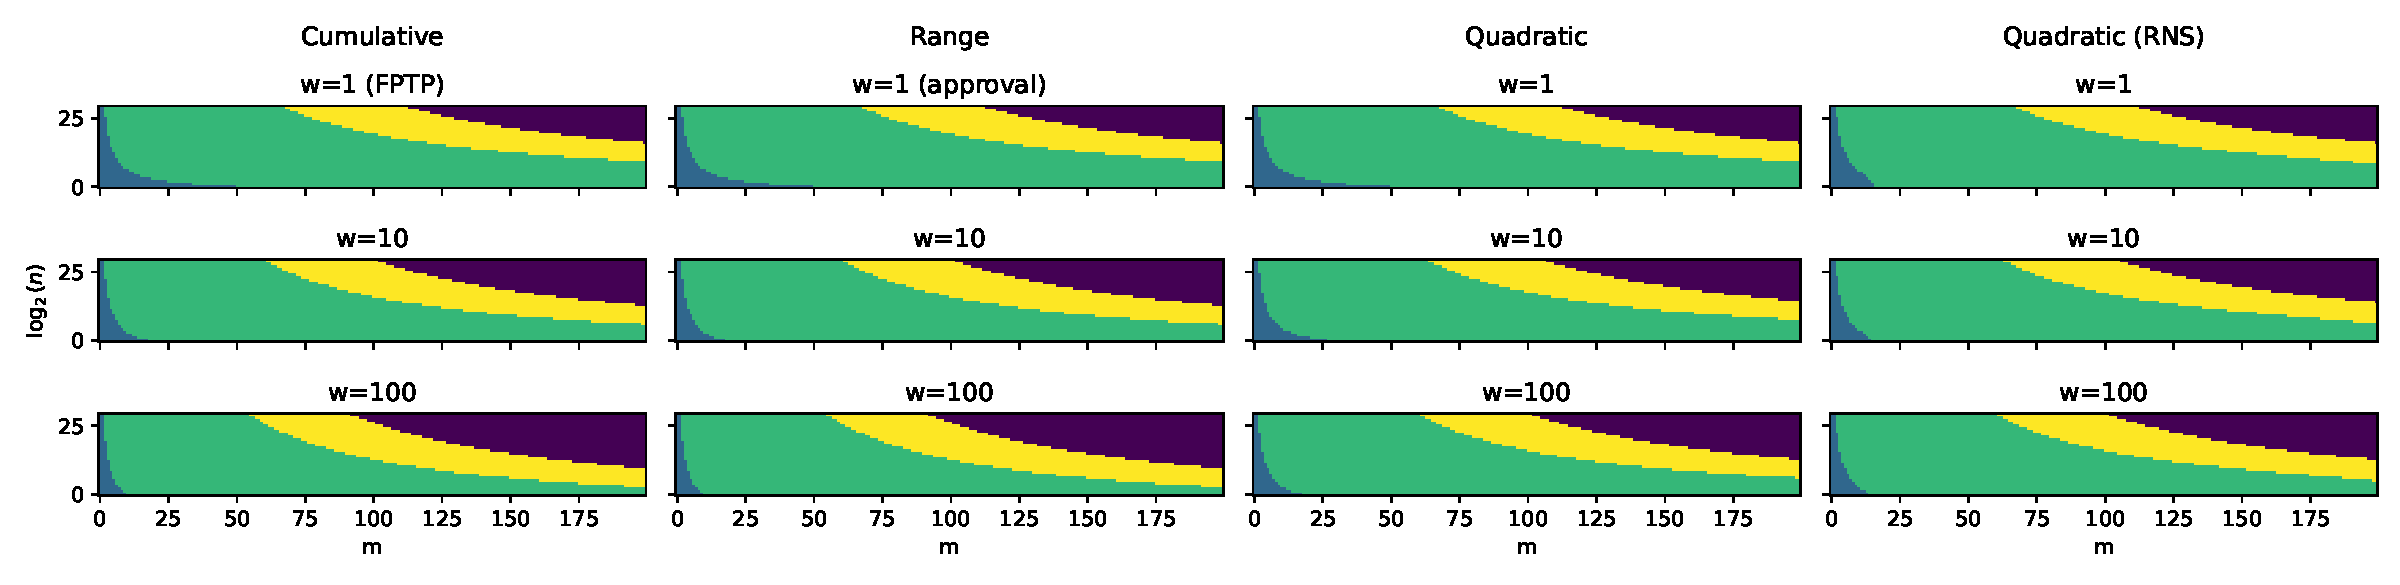
\includegraphics[width=\textwidth]{cicada/figs/params/pack_crq.pdf}
% \includegraphics[scale=0.56,trim={0.5cm 3cm 0.2cm 4.5cm},clip]
    \centering  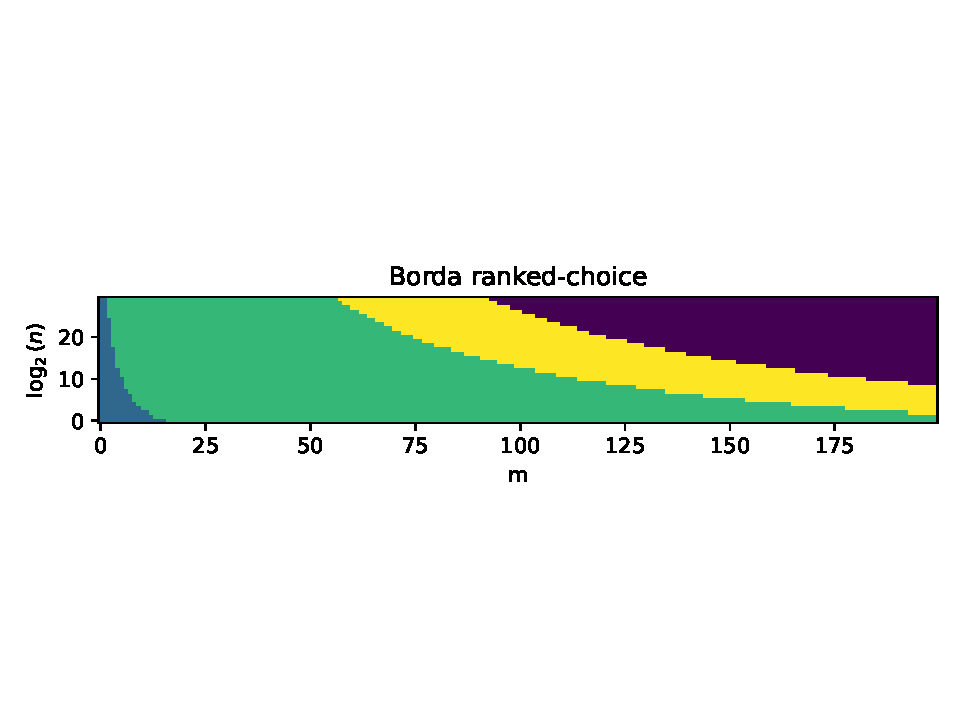
\includegraphics[width=0.45\textwidth,trim={0cm 3cm 0cm 4.5cm},clip]{cicada/figs/params/pack_borda.pdf}  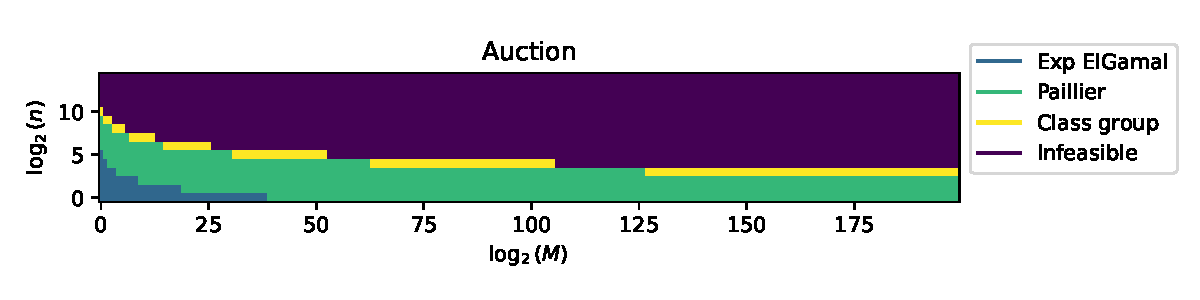
\includegraphics[width=0.5\textwidth,trim={0cm -1cm 0cm 4.5cm}]{cicada/figs/params/pack_auction.pdf}
    \caption{Most efficient HTLP construction for voting and auction using Cicada with maximal packing (using PNS except where indicated).}
    \label{fig:packed_feasibility}
\end{figure}

\begin{figure}[tb!]
    \centering
    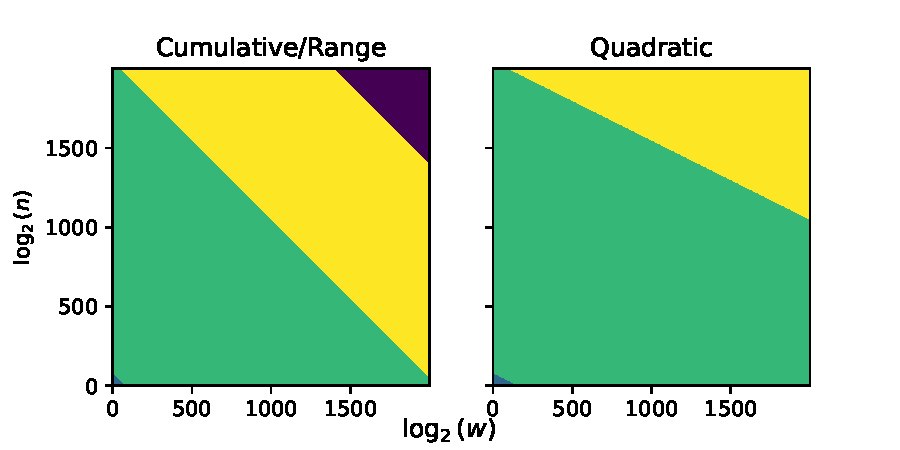
\includegraphics[width=0.49\textwidth,trim={0cm -0.5cm 0cm 0cm}]{cicada/figs/params/nopack_crq.pdf}
    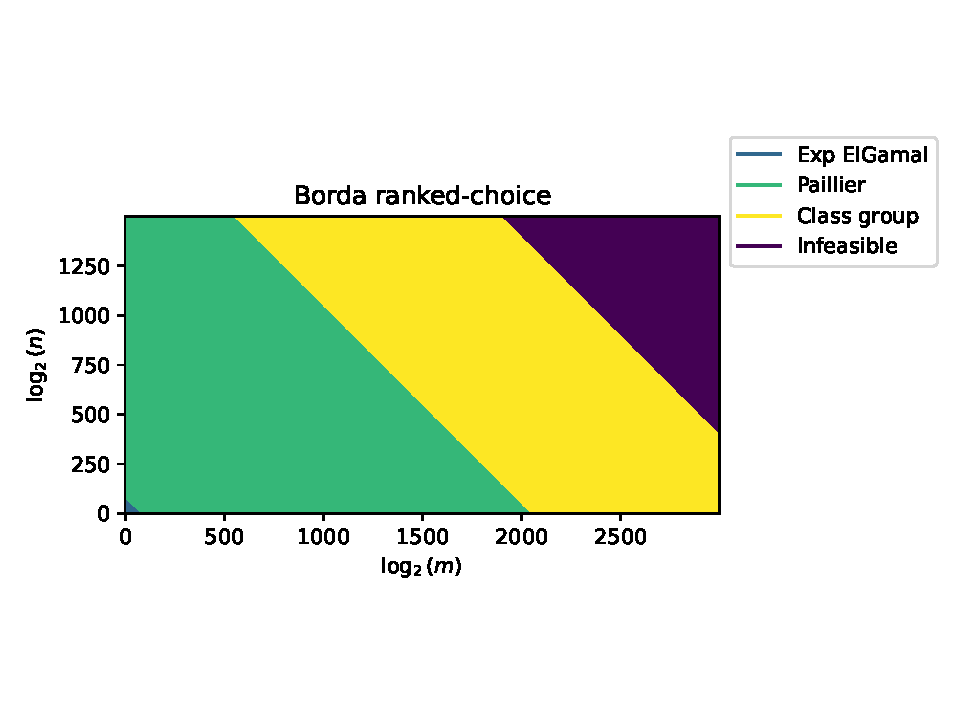
\includegraphics[width=0.49\textwidth,trim={2cm 2cm 0cm 2cm},clip]{cicada/figs/params/nopack_borda.pdf}
    \caption{Most efficient HTLP construction for voting schemes using Cicada without packing. For the sealed-bid auction, the bid bit-length directly determines the HTLP construction to use (exponential ElGamal up to 80 bits, then Paillier up to 2048, and class group up to 3400).}
    \label{fig:nopack_feasibility}
\end{figure}

\paragraph{Exponential ElGamal HTLP (\Cref{con:exp_elgamalHTLP})} 
This is the most efficient HTLP construction: for a given security parameter, it has the smallest required cryptographic groups and most efficient group operations. However, since the puzzle solution is encoded in the exponent, solving the puzzle requires brute-forcing a discrete logarithm. This limits the use of this construction to a small set of parameter settings: assuming the largest discrete logarithm an off-chain solver can be expected to brute-force has $\tau$ bits, we require $(nw+1)^m \leq 2^{2\tau}$.

\paragraph{Paillier HTLP (\Cref{con:paillierHTLP})} 
This is a slightly less efficient construction since the size of the HTLPs for a given security parameter is doubled due to working over $\bmod~N^2$ instead of $\bmod~N$. This increases both the required storage and the complexity of the group operation. On the other hand, due to its larger solution space, the Paillier HTLP supports much broader parameter settings for a given security parameter.

\paragraph{Class group HTLP} 
Class group offer the sole HTLP construction without a trusted setup~\cite{CCS:TCLM21}. This comes at the cost of the largest groups for a given security parameter. Class groups are not widely supported by major cryptographic libraries, and their costly group operation makes blockchain deployment difficult. We are unaware of any class group implementations for Ethereum smart contracts.

\paragraph{Impractical parameter settings} 
Accommodating very large settings of $n,\allowbreak w,m,M$ requires larger groups, leading to group operations and storage requirements which are intolerably inefficient for certain applications.
\section{Implementation}\label{sec:cicada_eval} 

\subsection{Parameter Settings}

In this section, we evaluate the practicality and optimality of various HTLP constructions based on the parameters $M,n,m,w$ of the auction or vote. 
% As discussed in~\Cref{sec:packing}, the size of the applied integer representations of ballots/bids increases linearly in certain parameters of the voting/auction schemes, e.g., the number of candidates. This limits the applicability of certain HTLP constructions instantiated in specific cryptographic groups, as we show next.  
Assuming the classic PNS packing, we require $(nw+1)^m\leq\vert\mathbb{G}\vert$ for voting and $M^n\leq\vert\mathbb{G}\vert$ for auctions, where $\mathbb{G}$ is the group in which the HTLP is instantiated.
We show the optimal HTLP construction for auctions and voting for various parameter settings in \Cref{fig:packed_feasibility} (with packing) and \Cref{fig:nopack_feasibility} (without packing). We use the security parameter $\secpar=80$ (see discussion in \Cref{sec:implementation}), which corresponds to a $1024$-bit modulus $N$ for exponential ElGamal and Paillier HTLPs and $3400$-bit discriminants for class group HTLPs. For the exponential ElGamal HTLP, we fixed the maximum ballot at $2^{80}$, which corresponds to $\approx 2^{40}$ brute-forcing work using Pollard's rho algorithm~\cite{Pollard78}.

\begin{figure}[tb!]
    \centering
    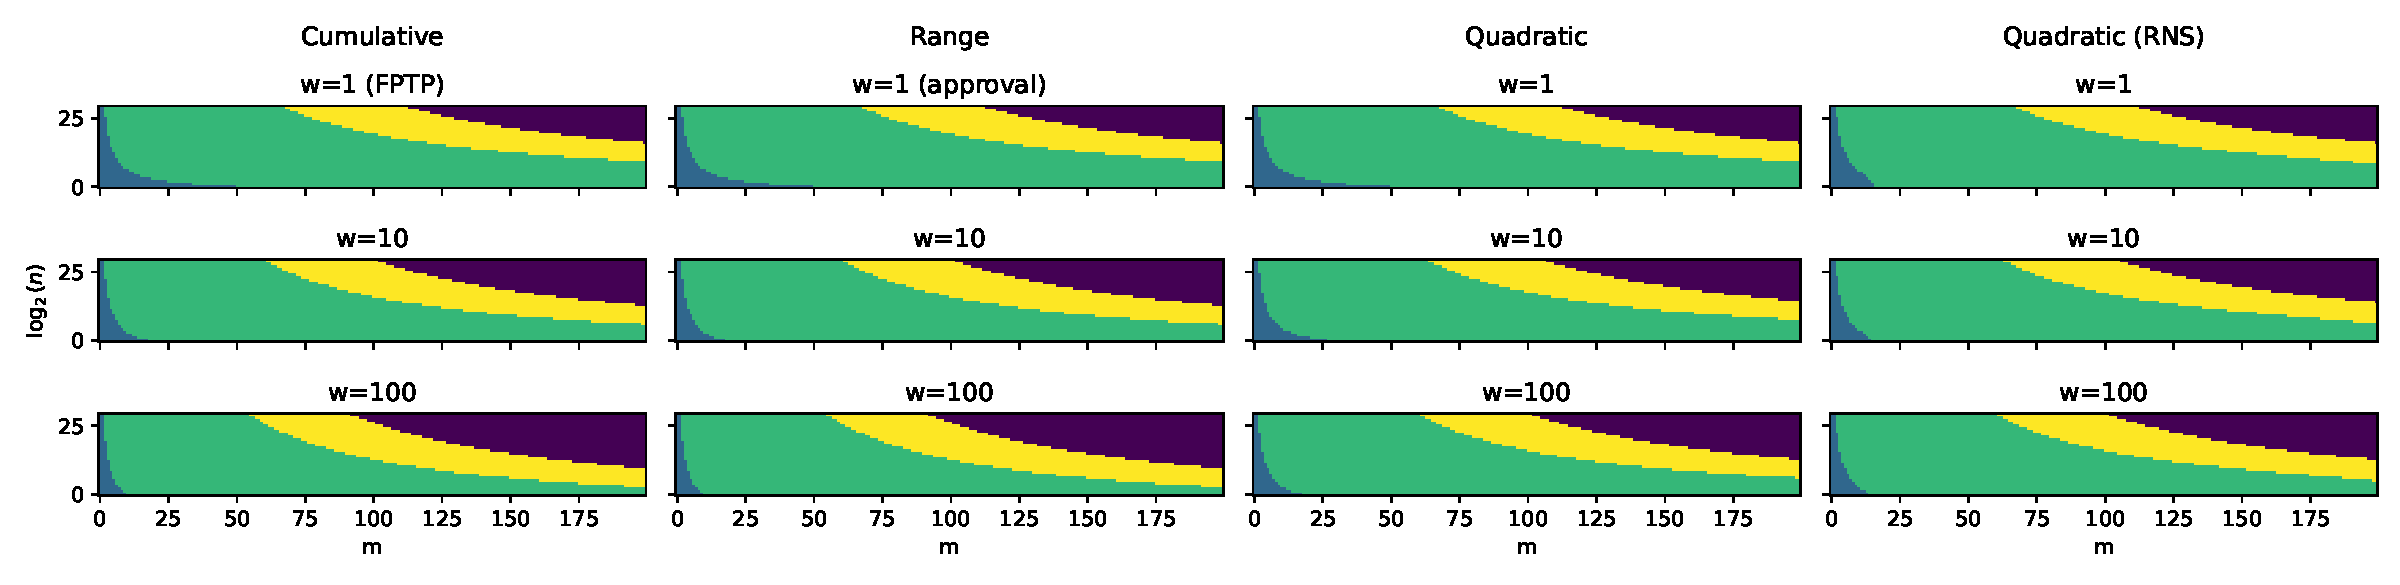
\includegraphics[width=\textwidth]{cicada/figs/params/pack_crq.pdf}
% \includegraphics[scale=0.56,trim={0.5cm 3cm 0.2cm 4.5cm},clip]
    \centering  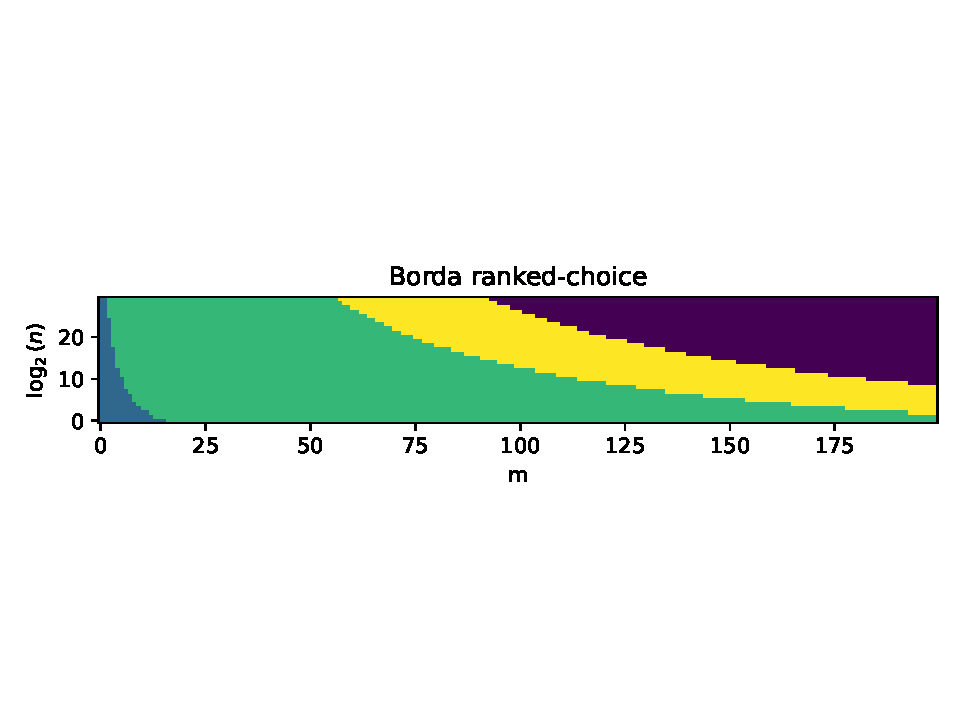
\includegraphics[width=0.45\textwidth,trim={0cm 3cm 0cm 4.5cm},clip]{cicada/figs/params/pack_borda.pdf}  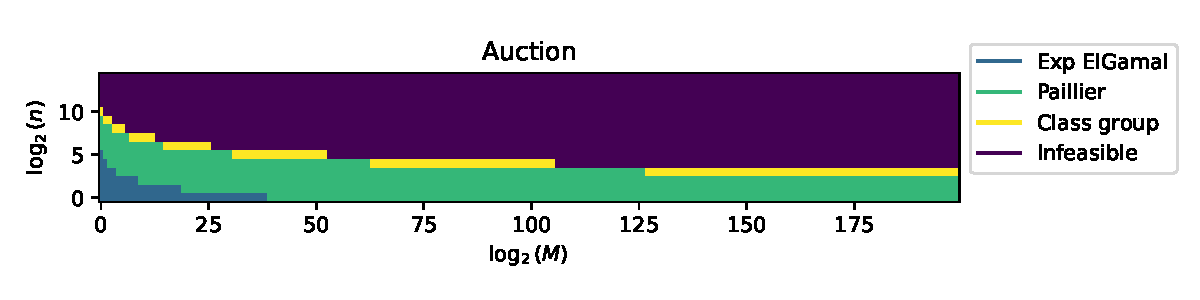
\includegraphics[width=0.5\textwidth,trim={0cm -1cm 0cm 4.5cm}]{cicada/figs/params/pack_auction.pdf}
    \caption{Most efficient HTLP construction for voting and auction using Cicada with maximal packing (using PNS except where indicated).}
    \label{fig:packed_feasibility}
\end{figure}

\begin{figure}[tb!]
    \centering
    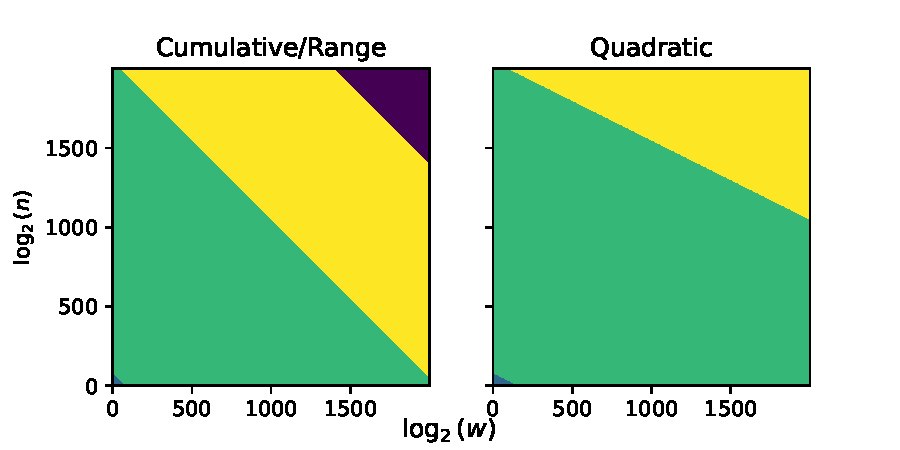
\includegraphics[width=0.49\textwidth,trim={0cm -0.5cm 0cm 0cm}]{cicada/figs/params/nopack_crq.pdf}
    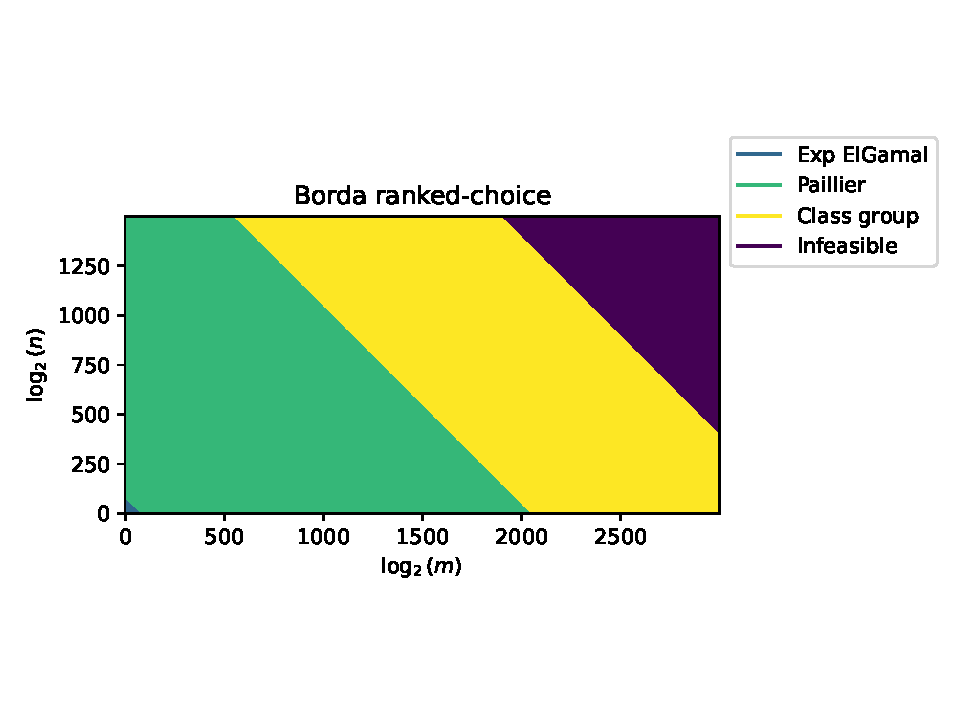
\includegraphics[width=0.49\textwidth,trim={2cm 2cm 0cm 2cm},clip]{cicada/figs/params/nopack_borda.pdf}
    \caption{Most efficient HTLP construction for voting schemes using Cicada without packing. For the sealed-bid auction, the bid bit-length directly determines the HTLP construction to use (exponential ElGamal up to 80 bits, then Paillier up to 2048, and class group up to 3400).}
    \label{fig:nopack_feasibility}
\end{figure}

\paragraph{Exponential ElGamal HTLP (\Cref{con:exp_elgamalHTLP})} 
This is the most efficient HTLP construction: for a given security parameter, it has the smallest required cryptographic groups and most efficient group operations. However, since the puzzle solution is encoded in the exponent, solving the puzzle requires brute-forcing a discrete logarithm. This limits the use of this construction to a small set of parameter settings: assuming the largest discrete logarithm an off-chain solver can be expected to brute-force has $\tau$ bits, we require $(nw+1)^m \leq 2^{2\tau}$.

\paragraph{Paillier HTLP (\Cref{con:paillierHTLP})} 
This is a slightly less efficient construction since the size of the HTLPs for a given security parameter is doubled due to working over $\bmod~N^2$ instead of $\bmod~N$. This increases both the required storage and the complexity of the group operation. On the other hand, due to its larger solution space, the Paillier HTLP supports much broader parameter settings for a given security parameter.

\paragraph{Class group HTLP} 
Class group offer the sole HTLP construction without a trusted setup~\cite{CCS:TCLM21}. This comes at the cost of the largest groups for a given security parameter. Class groups are not widely supported by major cryptographic libraries, and their costly group operation makes blockchain deployment difficult. We are unaware of any class group implementations for Ethereum smart contracts.

\paragraph{Impractical parameter settings} 
Accommodating very large settings of $n,\allowbreak w,m,M$ requires larger groups, leading to group operations and storage requirements which are intolerably inefficient for certain applications.

\subsection{Our Implementation}\label{sec:implementation}

We implemented our transparent on-chain coordinator as an Ethereum smart contract in Solidity.\footnote{Open-sourced at \url{https://github.com/a16z/cicada}.} 
For efficiency, we use the exponential ElGamal HTLP with a 1024-bit modulus $N$.
To enable 1024-bit modular arithmetic in $\ZZ_N^*$, we developed a Solidity library which may be of independent interest. 
This size of $N$ corresponds to approximately $\secpar=80$ bits of security.
Although this security level is no longer deemed cryptographically safe, the secrecy of the HTLP solutions is only guaranteed up to time $T$ regardless, so this security level will suffice for our use case as long as the best-known factoring attack takes at least $T$ time. A 2012 estimate for factoring 1024-bit integers is about a year~\cite{facthacks}, which is significantly longer than the typical submission period of a decentralized auction or election.

The main factors influencing gas cost (see \Cref{sec:cicada_costs}) are submission size, correctness proof size, and verification complexity. These factors mainly depend on the packing parameter $\ell\in[m]$, which determines a storage-computation trade-off with the following extremes:
% For the implementation, our main concern is minimizing the size of the ballots/bids, their correctness proofs, and the verification complexity of the correctness proofs. These metrics influence the gas cost efficiency of our transparent tallying authorities/auctioneers implemented as Ethereum smart contracts in Solidity. Our code is open-sourced.~\footnote{\url{https://github.com/a16z/cicada}\todo{anonymize}}

\begin{description}
    \item[One aggregate HTLP for all.] If $\ell=m$, the contract maintains a single aggregate HTLP $Z$. This greatly reduces the on-chain space requirements of the resulting voting or auction scheme at the expense of typically more complex and larger submission correctness proofs.
    \item[One aggregate HTLP per candidate.] If $\ell=1$, the contract must maintain $m$ aggregate HTLPs $\{Z_j\}_{j\in[m]}$. This increases the on-chain storage, but the submissions of correctness proofs become smaller and cheaper to verify.
\end{description}
In~\Cref{sec:cicada_costs}, we empirically explore this trade-off space by measuring the gas costs of various deployments of our framework with a range of parameter settings $M,n,m,w,\ell$.
% \joe{what about other points in the trade-off space?}
%\noemi{we don't actually measure any ``in-between'' settings of $\ell$ though, can we simulate or at least discuss whether it's linear?}\istvan{should be linear} 

First, we briefly describe the proof systems used for each scheme we implement; detailed descriptions are given in \Cref{sec:sigmas}.

\paragraph{Binary voting.} 
In a binary vote (i.e., approval voting with $m=1$), such as a simple yes/no referendum, users prove that the submitted ballot $Z=(u,v)$ is an exponential ElGamal HTLP with solution $0$ or $1$: $(u=g^r\land v=h^r)\lor(u=g^r\land vy^{-1}=h^r)$. This is achieved via OR-composition~\cite{C:CraDamSch94} of two sigma protocols for discrete logarithm equality~\cite{C:ChaPed92}.

\paragraph{Cumulative voting.}
In cumulative voting, each user distributes $w$ votes among $m$ candidates. To accommodate a larger number of candidates, our implementation keeps $m$ tally HTLPs $Z_j$, one for each candidate (in other words, $\ell = 1$). Each voter $i$ submits $m$ ballots $Z_{ij} = (g^{r_{ij}},h^{r_{ij}}y^{s_{ij}})$ for all $j\in[m]$. Besides proving (using the protocol \zkpoks) that each HTLP is well-formed (the same $r_{ij}$ is used in both terms), the voter must prove that $0 \leq s_{ij}~\forall\ j\in[m]$ and $\sum^m_{j=1} s_{ij}=w$. The first condition is shown with a proof of positive solution (\zkpopos) via Legendre's three-square decomposition theorem~\cite{ACNS:Groth05}. As a building block, we use a proof of square solution (\zkposqs) to show that a puzzle solution is a square. The second condition is proven by providing the randomness $R_i = \prod_j r_{ij}$ which opens $\prod_{j} Z_{ij}$ to $w$.

\paragraph{Sealed-bid auction.}
To illustrate two extremes of the packing spectrum, we implement two flavors of sealed-bid auctions. The first uses a single aggregate HTLP as described in \Cref{sec:cicada_framework} (this can be viewed as $\ell = b$, where $b = \ceil{\log_2(M)}$ is the bit-length of a bid): Bidder $i$ submits a single HTLP $Z_i = (g^{r_i},h^{r_i} y^{s_i})$, proving well-formedness with \zkpoks and two \zkpopos to show $0\leq s\leq M$. The coordinator aggregates the $i$th bidder's bid by adding $M^{i-1} \cdot Z_i$ to its tally.
% The coordinator will aggregate the $i$th bidder's bid by multiplying it by $2^{ib}$, where $b = \ceil{\log_2(M)}$ is the bit-length of the max bid $M$. That is each $b$-bit segment of the aggregate HTLP stores one bid. 

The second approach applies $b$ aggregate HTLPs (i.e., $\ell = 1$): Each bidder $i$ submits $b$ HTLPs $\{Z_{ij}\}_{j \in [b]}$ and uses the same proof system as in binary voting to prove their well-formedness, i.e., the user inserted for each bit of the bid $0$ or $1$. The coordinator adds $2^i \cdot Z_{ij}$ to each corresponding aggregate HTLP $Z_j$.%\footnote{We implement\noemi{check this} an optimization in which the bidders perform the scalar multiplication on behalf of the coordinator, proving instead $\forall j\in[b]$, $(u=g^r\land v=h^r)\lor(u=g^r\land vy^{-2^i}=h^r)$.\noemi{not sure if it's easy to discuss at which $M > 2$ this stops being more efficient than having the contract do the multiplication?}\istvan{doesn't the contract need to do the multiplication anyways because of security reasons? You cannot trust the user computing $y^{-2^i}$.}}\istvan{see signal conversation for more discussion on this.}
% We also describe the proof systems used for the implemented schemes in the full version.

\subsection{Deployment Costs}\label{sec:cicada_costs}

\begin{table*}[tb!]
    \makebox[\linewidth]{
    \centering
    \setlength{\tabcolsep}{6pt}
    \setlength{\belowbottomsep}{6pt}
    \begin{tabular}{l c ccccc}
        \toprule
        & \textbf{Binary vote} & \multicolumn{5}{c}{\textbf{Cumulative vote} ($\ell=1$)} \\\midrule
        $m$             & $1$ & $2$ & $3$ & $4$ & $5$ & $6$ \\\midrule
        \Aggr      & $418,358$ & $3,391,514$ & $5,081,542$ & $6,781,389$ & $8,489,786$ & $10,208,185$ \\
        \Finalize  & $115,690$ & $269,505$ &$397,789$&$521,895$&$644,814$&$770,934$ \\
        \midrule %%%%%%%%%%%%%%%%%%%%%%%%%%%%%%%%
        & \textbf{Sealed-bid auction} ($\ell = b$) & \multicolumn{5}{c}{\textbf{Sealed-bid auction} ($\ell=1$)} \\\midrule
        $b$                  & any & $8$ & $10$ & $12$ & $14$ & $16$ \\\midrule
        \Aggr                & $3,055,107$ & $3,586,022$ & $4,488,050$ & $5,394,047$ & $6,304,164$ & $7,218,905$ \\
        \Finalize            & $147,634$ & $1,005,208$ & $1,253,119$ & $1,497,760$ & $1,749,489$ & $2,003,282$ \\
        \bottomrule
    \end{tabular}
    }
    \caption{Gas costs for Cicada cumulative voting and sealed-bid auctions with various numbers of candidates $m$, bid bit-lengths $b$ (max. bid $M = 2^{b-1}$), and packing parameters $\ell$.}
    \label{tab:gas_table}
\end{table*}

We report EVM gas costs of several instantiations of Cicada in \Cref{tab:gas_table}. 

\paragraph{Submission costs} 
The on-chain cost of submitting a bid/ballot is the cost of running the $\sf Aggr$ function by the contract, i.e., the verification of the well-formedness proofs plus adding the users' submissions to the tally HTLPs (if and only if they verify). We report our measurements without packing (i.e., $\ell=1$). Submitting a binary vote ballot costs $418,358$ gas ($\approx 15.36$ USD on Ethereum).\footnote{We can estimate gas costs for approval voting using the cost of binary voting, as the former uses a disjunction of $m$ copies of the same NIZK and thus scales linearly.} 
For cumulative voting, the submission cost scales linearly in $m$: with $m=2$ candidates, submitting a ballot costs 
$3,391,514$ gas ($\approx124.51$ USD), 
and each additional candidate adds $\approx 1,699,847$ gas ($\approx 62.40$ USD).

An auction with a single HTLP for each bit of the bid (the $\ell=1$ case) requires a submission cost of $3,586,022$ gas ($\approx94.49$ USD) for an $8$-bit bid. Every additional bit in the submitted bid burns $\approx451,014$ gas ($\approx 11.89$ USD). 
On the other hand, if one applies packing, i.e., $\ell=b$, then the cost of submitting a sealed bid is constant at $3,055,107$ gas ($\approx131.65$ USD). With bid-space $M=2^7$ it is already more economical to have a single aggregate HTLP and use a packing scheme, despite more complex bid-correctness proofs.

\paragraph{Finalization costs} 
Our voting and auction schemes end with solving the tally HTLP(s) off-chain, i.e., computing $(g^r)^{2^{\Ttime}}$. With exponential ElGamal, solving the puzzle also requires the off-chain solver to brute-force a discrete logarithm. The correctness of this computation is proven to the contract with Wesolowski's \poe~\cite{EC:Wesolowski19} (recalled in \Cref{sec:sigmas}). The $\Finalize$ cost comes from verifying the \poe(s) on-chain, which burns $101,066$ gas ($\approx3.71$ USD) per proof. Without packing, the untrusted solver must provide a Wesolowski proof per tally HTLP, so the $\Finalize$ gas cost is linear in the number of tally HTLPs. A portion of the Wesolowki verification cost comes from checking that the challenge is a prime number. Our implementation uses a Baillie-PSW~\cite{PomSelWag80} primality test, which costs $44,972$ gas ($\approx1.65$ USD). 

\begin{table}[ht]
    \centering
    \setlength{\tabcolsep}{6pt}
    % \setlength{\belowbottomsep}{6pt}
    \begin{tabular}{l r}
       \toprule
       \textbf{Sigma protocol}  & \textbf{Verification gas cost}\\
       \midrule
       Proof of Exponentiation (\poe~\cite{EC:Wesolowski19})& $101,066$\\
        PoK of solution (\zkpoks) & $266,096$ \\
        Proof of solution equality (\zkposeq) & $336,155$ \\
        Proof of square solution(\zkposqs) & $336,168$ \\
        Proof of positive solution (\zkpopos) & $1,351,958$ \\
        \bottomrule
    \end{tabular}
    \caption{EVM gas costs of verification for the proof systems described in~\Cref{sec:sigmas}.}
    \label{tab:sigmas_gas}
\end{table}

\paragraph{Verification costs}
Our Solidity implementation includes the sigma protocols described in \Cref{sec:sigmas}. We report their verification costs in~\Cref{tab:sigmas_gas}. With Groth's trick~\cite{ACNS:Groth05} in the proof of positivity (\zkpopos), we must decompose the integer solution into the sum of only three squares. Therefore, the gas cost of verifying \zkpopos equals the cost of verifying three proofs of knowledge of square solutions (\zkposqs) and one proof of knowledge of equal solution (\zkposeq).

\begin{table*}[ht!]
    % \adjustbox{width=1.2\textwidth,center}{
    \centering
    \setlength{\tabcolsep}{6pt}
    \setlength{\belowbottomsep}{6pt}
    \begin{tabular}{l SS}
        \toprule
        & {\textbf{Binary vote}} & {\textbf{Sealed-bid auction} ($\ell = b$)} \\\midrule
        & {$m=1$} & {$b=$ any} \\\midrule
        $\Aggr$\ (ETH L1)     & 15.36 & 112.16 \\
        $\Aggr$\ (Arbitrum Nova)      & 0.35 & 2.55 \\
        $\Aggr$\ (Optimism)      & 0.00918 & 0.06701 \\
        $\Aggr$\ (zkSync Era)     & 0.063 & 0.459 \\\midrule
        $\Finalize$\ (ETH L1)  & 4.25 & 5.42 \\
        $\Finalize$\ (Arbitrum Nova)  & 0.10 & 0.12 \\
        $\Finalize$\ (Optimism) & 0.00254 & 0.00324 \\
        $\Finalize$\ (zkSync Era)  & 0.017 & 0.022 \\
        \bottomrule
    \end{tabular}
    \caption{USD costs of Cicada binary vote and fully packed ($\ell=b$) sealed-bid auction on Ethereum L1, Arbitrum Nova, Optimism, and zkSync Era as of July 30, 2024 at 7:30 PM UTC.}
    \label{tab:usd_table1}
\end{table*}

\begin{table*}[ht!]
    % \makebox[\linewidth]{
    % \resizebox{1.2\textwidth}{!}{
    \adjustbox{width=1.2\textwidth,center}{
    \centering
    \setlength{\tabcolsep}{6pt}
    \setlength{\belowbottomsep}{6pt}
    \begin{tabular}{l SSSSS}
        \toprule
        & \multicolumn{5}{c}{\textbf{Cumulative vote} ($\ell=1$)} \\\midrule
        $m$             & {2} & {3} & {4} & {5} & {6} \\\midrule
        $\Aggr$\ (ETH L1)     & 124.51 & 186.55 & 248.95 & 311.67 & 374.75 \\
        $\Aggr$\ (Arbitrum Nova)      & 2.83 & 4.24 & 5.66 & 7.08 & 8.52 \\
        $\Aggr$\ (Optimism)      & 0.07439 & 0.11145 & 0.14874 & 0.18621 & 0.22390 \\
        $\Aggr$\ (zkSync Era)     & 0.509 & 0.763 & 1.018 & 1.275 & 1.533 \\\midrule
        $\Finalize$\ (ETH L1)  & 9.89 & 14.60 & 19.16 & 23.67 & 28.30 \\
        $\Finalize$\ (Arbitrum Nova)  & 0.22 & 0.33 & 0.44 & 0.54 & 0.64 \\
        $\Finalize$\ (Optimism) & 0.00591 & 0.00872 & 0.01145 & 0.01414 & 0.01691 \\
        $\Finalize$\ (zkSync Era)  & 0.040 & 0.060 & 0.078 & 0.097 & 0.116 \\
        \midrule
        & \multicolumn{5}{c}{\textbf{Sealed-bid auction} ($\ell=1$)} \\\midrule
        $b$                  & {8} & {10} & {12} & {14} & {16} \\\midrule
        $\Aggr$ (ETH L1)                & 131.65 & 164.76 & 198.02 & 231.43 & 265.01 \\
        $\Aggr$ (Arbitrum Nova)                & 2.99 & 3.74 & 4.50 & 5.26 & 6.02 \\
        $\Aggr$ (Optimism)                & 0.07865 & 0.09844 & 0.11831 & 0.13827 & 0.15833 \\
        $\Aggr$ (zkSync Era)                & 0.539 & 0.674 & 0.810 & 0.947 & 1.084 \\\midrule
        $\Finalize$ (ETH L1)            & 36.90 & 46.00 & 54.98 & 64.23 & 73.54 \\
        $\Finalize$ (Arbitrum Nova)            & 0.84 & 1.05 & 1.25 & 1.46 & 1.67 \\
        $\Finalize$ (Optimism)            & 0.02205 & 0.02748 & 0.03285 & 0.03837 & 0.04394 \\
        $\Finalize$ (zkSync Era)            & 0.151 & 0.188 & 0.225 & 0.263 & 0.301 \\
        \bottomrule
    \end{tabular}
    }
    \caption{USD costs of unpacked ($\ell=1$) Cicada cumulative voting and sealed-bid auctions for various settings of $m, b$ on Ethereum L1, Arbitrum Nova, Optimism, and zkSync Era as of July 30, 2024 at 7:30 PM UTC.}
    \label{tab:usd_table2}
\end{table*}

\paragraph{USD cost estimates on L1 and L2}
In the short-term, deploying on Layer 2 (L2) already brings the costs down by 1--2 orders of magnitude. 
In \Cref{tab:usd_table1,tab:usd_table2}, we provide a rough estimate of the concrete cost in USD as of July 30, 2024 of deploying Cicada on Ethereum and several Layer-2 (L2) networks. These numbers are conversions of the gas costs in \Cref{tab:gas_table} and should not be viewed as precise costs predictions, but rather as evidence of Cicada's concrete efficiency and feasibility. Precisely benchmarking costs in terms of USD is difficult due to the volatility of both the ETH/USD price and of transaction/priority fees on Ethereum and its L2s.
At the time of conversion (July 30, 2024 at 7:30 PM UTC), the Ethereum price was $0.00000333736$ USD per gwei and a medium priority fee on Ethereum L1 was $11$ gwei. We also consider three popular Ethereum rollups: Arbitrum Nova, Optimism, and zkSync Era. At the time of our measurement, transaction fees for Arbitrum Nova, Optimism, and zkSync Era were $0.25$, $0.006572$ and  $0.045$ gwei, respectively. 

While possible, our Cicada deployments are overall prohibitively expensive on Ethereum L1. However, the costs are quite reasonable on its L2s: participating in a Cicada sealed-bid auction, cumulative vote, or binary vote would cost less than $1$ USD on these popular Ethereum L2s, which we deem highly practical.
For example, when deploying our implementation on the Optimism L2 rollup, casting a binary vote would cost less than 0.30 USD.
Further optimizations (e.g., Karatsuba multiplication~\cite{KarOfm62}, batched Wesolowski proof verification~\cite{TCC:Rotem21}, or verification via efficient zkSNARKs~\cite{EC:Groth16,EPRINT:GabWilCio19}) can bring the costs down even more.
\subsection{Extensions}\label{sec:cicada_extensions}
We introduce extensions to the Cicada framework that may be useful in future applications.

\subsubsection{Everlasting ballot privacy for HTLP-based protocols}\label{sec:everlasting_ballot_privacy}

\begin{figure}
    \centering
    \begin{mdframed}
    \begin{center}
        \textbf{Off-chain batching}
    \end{center}
    \hfill\\
    \textbf{Public parameters:} A semiprime $N$ and $h, y \in \ZZ_N^*$, a voting scheme $\Sigma : \X^n \rightarrow \Y$. \hfill\\
    \newline
    Let $P_1, \dots, P_{k}$ be a group of $k < n$ parties with addresses ${\sf addr}_1, \dots, {\sf addr}_{k}$ wishing to batch their ballots $(u_i, v_i) := (g^{r_i}, h^{r_i} X_i)$.
    \begin{enumerate}
        \item Each party broadcasts $v_i$. Now, every party can compute $v := \prod_i v_i = h^R X$, which encodes the sum of their submissions.
        \item The parties use an $k-1$ malicious-secure MPC protocol~\cite{ESORICS:DKLPSS13,CCS:Keller20} on inputs $u_i$ to compute $u := \prod_i u_i = g^R$.
        \item They also compute two distributed-prover zero-knowledge proofs~\cite{PoPETS:DPPSV22} in the MPC: (i) a discrete logarithm equality proof $\pi_R$ that $\mathsf{dlog}_g(u) = \mathsf{dlog}_h(v)$ with distributed witness $R$, and (ii) a submission correctness proof $\pi_s$ that the aggregated solution $s$ encoded in $X$ is consistent with the sum of $k$ valid submissions, i.e., $s\in k \cdot \mathcal{X}$. Let $\pi_{\sf batch} = (\pi_R, \pi_s)$.
        \item Finally, each party signs the final aggregated submission $Z_{\sf batch} = (u,v)$.
    \end{enumerate}
    \textbf{Output}:~$(Z_{\sf batch},\pi_{\sf batch}, \{{\sf addr}_1, \dots, {\sf addr}_{k}\}, \{\sigma_1, \dots, \sigma_{k}\})$.
    
    \end{mdframed}
    \begin{mdframed}
    \begin{center}
        \textbf{On-chain batched ballot submission}
    \end{center}
    \hfill\\
    % batching only the first component
    % \textbf{Public parameters:} Cicada public parameters $\pp$. \hfill\\
    % \begin{enumerate}
    %     \item Parties $P_1, \dots, P_n$ wishing to batch their ballots submit $(g^0, h^{r_i} X_i)$ and a proof $\pi_i$ of well-formedness of the second component to the tallying contract (except leader $P_1$, who does nothing).
    %     \item $P_1, \dots, P_n$ execute the off-chain batching protocol (below), which outputs $g^R = \prod_{i \in [n]} g^{r_i}$ and $\pi_{batch}$ to $P_1$.
    %     \item $P_1$ submits $(g^R, h^{r_1} X_1)$ and proofs $\pi_1, \pi_{batch}$ by time $T-\tau$.
    %     \item If $P_1$ fails to submit by time $\tau$ or submits an inconsistent/invalid HTLP, the remaining parties re-run the off-chain batching protocol to compute $g^{R'} = \prod_{i \in [n], i \neq 1} g^{r_i}$ and a new proof $\pi_{batch}'$. Any (single) party $i^* \in [n]\setminus \{1\}$ can now override its submission with a new HTLP $(g^{R'}, h^{r_{i^*}} X_{i^*})$ and $\pi_{batch}'$. The second component should be the same as in the previous submission, and cheating can be punished by slashing.
    % \end{enumerate}
    \textbf{Public parameters:} Cicada public parameters $\pp$. \hfill\\
    \begin{enumerate}
        \item The designated party $P_1$ submits $Z_{\sf batch}, \pi_{\sf batch}, \{{\sf addr}_1, \dots, {\sf addr}_{k}\},\allowbreak \{\sigma_1, \dots, \sigma_{k}\}$ to the tallying contract, which verifies the proofs and signatures, and adds $(u,v)$ to the tally HTLP $Z$ as in the basic protocol.
        \item If $P_1$ doesn't submit by time $T-\tau$, any other party in the batch group can submit instead.
    \end{enumerate}
    \end{mdframed}
    
    \caption{The on- and off-chain ballot batching protocols that $k < n$ parties can use to achieve everlasting ballot privacy.}
    \label{fig:batching_ballots}
\end{figure}

\noemi{Note this introduces interactivity but off-chain}

The basic Cicada framework does not guarantee long-term ballot privacy. Submissions are public after the $\Open$ stage. This is because users publish their HTLPs on-chain: once public, the votes contained in the HTLPs are only guaranteed to be hidden for the time it takes to compute $\Ttime$ sequential steps, after which point it is plausible that someone has computed the solution. In many applications, it is desirable that individual ballots remain hidden \emph{even after voting has ended} since the lack of everlasting privacy may facilitate coercion and vote-buying. As mentioned in \Cref{sec:syntax}, this can be achieved modularly by first decoupling the ballots from their voters via a privacy-enhancing overlay. Alternatively, we describe how the $\Seal$ procedure can be modified to prevent the opening of individual ballots, achieving everlasting privacy.

Observe that all known \emph{efficient HTLP constructions} are of the form $(u,v) = (g^r, {h'}^r X)$,\footnote{In the exponential ElGamal case, $h' = h$, while in the Paillier construction, $h' = h^N$ (see \Cref{app:htlp_constructions}). We will drop the tickmark on $h'$ in the remainder of this section to avoid notational clutter.} where the solution is encoded in $X$ and recovering it requires recomputing $h^r=(g^{r})^{2^{\Ttime}}$ via repeated squaring of the first component. Our insight is that the puzzle information-theoretically hides the solution $X$ without the first component. Importantly, publishing $g^r$ is not necessary in any of our HTLP-based voting protocols \emph{except as a means to verifiably compute the first component of the final HTLP}, i.e., $g^{R}=g^{\sum_{i\in[n]} r_i}$. The observation that $g^R$ can be computed \emph{without} revealing the individual values $g^{r_i}$ enables us to construct the first practical and private voting protocols that guarantee \emph{everlasting} ballot privacy with a single on-chain round.

% \todo{change text starting around here...} \noemi{Note you can use aggregatable sigs for efficiency}
For simplicity, consider a protocol in which both the ballot of user $i$ and the tally consists of a single HTLP, respectively $Z_i=(g^{r_i},h^{r_i}X_i)$ and $Z = (g^R, h^R X)$. Observe that for everlasting ballot privacy, updates to $Z$ must inherently be batched: a singleton update $\Aggr(\pparam, Z, Z_i, \pi) \to (g^{R+r_i}, h^{R+r_i} Y)$ (for some $Y$) would reveal $g^{r_i} = g^{R+r_i}/g^R$, which is the opening information to $Z_i$, as the quotient of the first component of $Z$ after and before the update. Hence, the ballot $X_i$ of user $i$ would be recoverable in $\Ttime$ sequential steps, i.e., after computing $h^{r_i}=(g^{r_i})^{2^{\Ttime}}$.

Batching ballot submissions off-chain in groups of $k$ allows parties to achieve everlasting privacy as long as at least one party is honest. 
The parties aggregate their submissions off-chain as $(g^R, h^R X) = (\prod_i g^{r_i}, \prod_i h^{r_i} X_i)$ and compute a proof $\pi_{\sf batch}$ of well-formedness in a distributed-prover zero-knowledge proof protocol~\cite{PoPETS:DPPSV22}. We use the observation that the individual second components $v_i$ are hiding to optimize the batching by computing $h^R X$ in the clear
% Intuitively, the parties compute their aggregate randomness $g^R = \prod_i g^{r_i}$ and a proof $\pi_{\sf batch}$ of its well-formedness in a distributed-prover zero-knowledge proof protocol~\cite{dayama2021prove}. Each party submits only the second component of its ballot to the contract, except a designated party (e.g., $P_1$) who also submits $g^R$. The updated tally HTLP $Z^*$ is computed as 
% $\Aggr(\pparam, Z, \{(g^R, h^{r_1} X_1),\allowbreak (g^0, h^{r_2} X_2), \dots,\allowbreak (g^0, h^{r_k} X_k) \}, \pi_{\sf batch}),$
% where $\pi_{\sf batch}$ additionally proves to the contract that ${\sf dlog}_g(g^R) = {\sf dlog}_h(\prod_i h^{r_i} X_i)$, 
(see~\Cref{fig:batching_ballots} for details).

\begin{figure}[htb]
    \centering
    \begin{mdframed}
    \begin{center}
        \textbf{Borda ballot correctness}
    \end{center}
    \todo{incomplete}
    \begin{enumerate}
       \item $\mathcal{P}$ sends $(g^a\bmod{N},(1+N)^{a}\bmod{N^2})$ for $a\sample\mathbb{Z}_N$. 
       \item $\mathcal{V}$ sends a challenge $e\sample[1,n]$.  
       \item $\mathcal{P}$ sends $(g^{r\cdot e+a},h^{r\cdot N\cdot e+a}(1+N)^{s\cdot e+a}\bmod{N^2})$.
    $\mathcal{V}$ accepts iff the following hold:
    \end{enumerate}
    \end{mdframed}
    \label{fig:borda-pok}
\end{figure}


This idea opens up a new design space for the MPC protocol used for batching, such as doing the randomness generation in a preprocessing phase instead, allowing dynamic additions to the anonymity set, optimizing the batch proof generation, and dealing with parties who fail to submit. We leave the full exploration of this large design space and related questions to future work.

% As an alternative, the MPC could be run in a pre-processing stage which outputs a random $t$-of-$n$ sharing of a uniform $R$ and the proof $\pi_{\sf batch}$. Once party $i$ is ready to submit, it computes $Z_i = h^{r_i} X_i$ and sends it to the contract as above.

% The protocol is described in detail in \Cref{fig:batching_for_everlasting_privacy}.
% For $k$ parties holding ballots $Z_i = (g^{r_i}, h^{r_i} X_i), i \in [k]$, each party hides the first component of its ballot by computing $Z_i' = (g^{r_i}h^{u_i}, h^{r_i} X_i)^{k}_{i=1}$ for some $u_i\sample\mathbb{Z}_N$. Next, the parties run a secure multi-party computation (MPC) protocol (in the 2-party case, they just run this in the clear) to compute $g^{R}h^{U} = g^{\sum_i r_i}h^{\sum_i u_i}$. Then they open this commitment to $g^R$ by computing the opening information $h^U=\prod\limits^k_{i=1} h^{u_i}$ in MPC. $P_i$ will submit $(h^{r_i} X_i, \pi_i)$ to the contract, where $\pi_i$ is the original proof of puzzle well-formedness. Without loss of generality, let $P_1$ additionally send $g^R$. The updated tally $\htlp$ $Z^*$ is computed as $\Aggr(\pparam, Z^*, \{(g^R, h^{r_1} X_1), (g^0, h^{r_2} X_2), \dots, (g^0, h^{r_k} X_k) \}, \pi_{\sf batch})$, where $\pi_{\sf batch}$ additionally proves to the contract that ${\sf dlog}_g(g^R) = {\sf dlog}_h(\prod_i h^{r_i} X_i)$. % have the same discrete logarithms with respect to the bases $g$ and $h$, respectively.
    
% \todo{(before bids/ballots are fixed) and run an MPC to produce a random $t$-of-$n$ sharing (output $r_i$ to $P_i$ along with a proof $\pi_{r_i}$). As long as there are $n_0 > t$ parties to start, additional parties could join dynamically. Once a party is ready to submit, it computes $Z_i = (g^{r_i}, h^{r_i} X_i)$ and sends it to the contract as usual along with $\pi_{r_i}$, see Figure~\ref{fig:batching_for_everlasting_privacy}. Ballots must be accumulated by homomorphically reconstructing $r$, so this may rule out some class of functions over the $X_i$'s. This version is more resilient to dropouts since it can tolerate up to $n-t$ users not submitting their puzzles. The drawback is that the submissions are larger.}

% \begin{figure}[htb]
% \begin{mdframed}
% \begin{center}
%     \textbf{Privacy-preserving batching of ballots} 
% \end{center}
% \textbf{Public parameters:} Group of unknown order $\GG$ with  $g,h\sample\GG$, batch size $k$.\hfill\\
% \textbf{Public input:} The second component $h^{r_i} X_i$ of each voter's ballot, $i \in [k]$.\hfill\\
% \textbf{Private input:} The first component $g^{r_i}$ of each voter's ballot, $i \in [k]$.
% \begin{enumerate}
%     \item Each voter $i$ publishes $g^{r_i}h^{u_i}$ for $u_i \sample \ZZ$ along with a proof $\pi_i' \gets \Pi_{\sf PoEqDLog}.{\sf Prove}(g,g^{r_i}h^{u_i},h,h^{r_i} X_i; r_i)$.
%     \item Every party checks every other party's proof $\pi_i'$ and reconstructs $g^{R}h^{U}:=\prod^{k}_{i=1} g^{r_i}h^{u_i}$. (If any proof fails to verify, that party is excluded from the batch. \todo{check this doesn't intro predictable bias like Pedersen DKG})
%     \item The parties participate in an MPC to compute $h^U=\prod^{k}_{i=1}h^{u_i}$ and obtain $g^R=g^{R}h^{U}/h^{U}$.
%     \item Each party uses $h^U$ to compute $g^R = (g^R h^U)/h^U$. The parties collaboratively compute $\pi_{batch} \gets \Pi_{\sf PoEqDlog}.{\sf Prove}(g,g^R,h,\prod h^{r_i}X_i; R)$.
%     \item Each voter computes its ballot correctness proof $\pi_i$ for $h^{r_i} X_i$.
% \end{enumerate}
% \textbf{Output:} $(h^{r_i} X_i,\pi_i)^{k}_{i=1},g^R,\pi_{batch}$.

% \end{mdframed}
% \caption{Off-chain batching protocol for everlasting ballot privacy.}
% \label{fig:batching_for_everlasting_privacy}
% \end{figure}

% For simplicity, consider a protocol in which each user submits a single HTLP $Z_{\sf userID} := (Z_{\sf userID}^{(0)}, Z_{\sf userID}^{(1)})$ to the contract. With this modification, the user would instead submit only the second component $Z_{\sf userID}^{(1)}$ along with some masked version of the first component. \noemi{unclear how best to avoid leaking $\Delta r$ when the before/after of the update is known in the clear (e.g., if the accumulated vote HTLP is currently $g^{r_t}$, and after your update it's $g^{r_{t+1}}$, your update is easily deducible as $g^{r_{t+1}}/g^{r_{t}}$)... solutions could be batching updates (parties incentivized to batch anyway to reduce fees) or distributing shares of 1 at some point and weighting contribution by share.}

% \subsection{Adding Coercion Resistance}\label{sec:coercion_resistance}
% In certain applications, it is desirable to provide coercion-resistance~\cite{juels2005coercion} for the voters.
% \istvan{todo: for each user the contract stores their latest ballot. They can add the ``negative'' of their previous ballot to the tally. And now the user just needs to submit their new ballot which is subsequently added to the tally. The cost of this approach is that now all the votes need to be stored in the storage which might add $\approx 200,000$ gas more per ballot for the first submission.}
% Another potential solution might be to add the ballot randomizers to an accumulator/zero-knowledge sets.

% \todo{there is an impossibility result (\url{https://hackingdistributed.com/2018/07/02/on-chain-vote-buying/}) that coercion-resistance in the permissionless setting requires trusted hardware (trusted setup)}

\subsubsection{Succinct ballot-correctness proofs}\label{sec:succinct_ballot_correctness}

Real-world elections often have hundreds of candidates, e.g., Optimism's retroactive public good funding~\cite{retropgf_voterguide}. However, the state-of-the-art ballot correctness proofs~\cite{C:BBCGI23,ACNS:Groth05} for all voting schemes (e.g., FPTP, approval voting, etc.) are linear in the number of candidates, rendering these schemes impractical in the blockchain setting. To counter these issues, we design constant-size ballot correctness proofs with constant verification time at the expense of an added preprocessing phase. The high-level idea is as follows. All correct ballots (e.g., $\{ \pack(s) : s\in\{0,1\}^{m}\}$ in the case of approval voting) are inserted into an accumulator or polynomial commitment (PC)~\cite{AC:KatZavGol10} during a transparent preprocessing phase. When users submit their votes $Z \sample \htlp.\mathsf{Gen}(s)$, they prove in zero-knowledge that $Z$ encodes a correct ballot, i.e., the users show that the solution $s$ of $Z$ had been previously inserted into the accumulator or PC with a succinct (blinded) membership proof~\cite{CCS:ZBKMNS22}.
% We detail our succinct ballot-correctness proof using the KZG commitment in \Cref{app:succinct}.

In this section, we assume that a common reference string for the KZG polynomial commitment (PC) scheme~\cite{AC:KatZavGol10} is already available to users, namely $\mathsf{crs}:=\{g_1^{\tau^{j}}\}^{d}_{j=1}$, where $g_1\in\mathbb{G}_1$ is a generator in a bilinear pairing-friendly cyclic group $\mathbb{G}_1$ over $\mathbb{F}_p$ for some prime $p$, $\tau\sample\mathbb{F}_p$ hidden to everyone. The $\mathsf{crs}$ is typically established during a sequential, secure multi-party computation (MPC), e.g.,~\cite{FCW:BowGabGre18}.

%-----------------------------------------------------------BEGIN Preprocessing Ballots --------------------------------------------------------------
\begin{figure}
    \centering
    \begin{mdframed}
    \begin{center}
        \textbf{Preprocessing ballots for succinct ballot-correctness proofs}
    \end{center}
    \hfill\\
    \textbf{Public parameters:} The common reference string $\mathsf{crs}:=\{g_1^{\tau^{j}}\}^{d}_{j=1}\in\mathbb{G}_1^{d}$. A semiprime $N$ and $h, y \in \ZZ_N^*$. A voting scheme $\Sigma : \X^n \rightarrow \Y$, e.g., approval voting. \hfill\\
    \begin{enumerate}
        \item Let $\X$ be the set of correct ballots and $\vert\X\vert=d$
        \item Let $f(x)\in\mathbb{F}^{\leq d}_p[x]$ be a univariate polynomial s.t. $\forall s_i\in\X:f(i):=\pack(s_i)$. The polynomial $f(x)$ could be computed using Lagrangian interpolation.
        \item Let $\mathsf{com}$ be the KZG commitment to the polynomial $f$.
    \end{enumerate}
    \textbf{Output}:~$\mathsf{com}$.
    
    \end{mdframed}
    \caption{Preprocessing ballots to enable succinct ballot-correctness proofs.}
    \label{fig:preprocessing_ballots}
\end{figure}
%-----------------------------------------------------------END Preprocessing Ballots --------------------------------------------------------------

Let us assume that users have established during a preprocessing phase (\Cref{fig:preprocessing_ballots}) a short commitment $\mathsf{com}$ that encodes all the possible ballots in a particular voting scheme, e.g., $\X= [0,1]^{m}$ for approval voting. The size of classical proofs of well-formedness, e.g., OR-composition of sigma-protocols, scale linearly in the number of candidates $m$. The following proof strategy yields a constant-size proof of correctness for moderately-sized $\X$, i.e., $\sizeof{\X} \leq d$\footnote{The largest KZG CRS we know of~\cite{largekzg} is for $d = 2^{28}$, so in the case of $\X = [0,1]^m$ this strategy requires $m \leq 28$.}.
% $m$, say $m\leq 30$, depending on the size of the available  $\mathsf{crs}$ of the polynomial commitment scheme.

First, given a ballot $Z=(g^r,h^ry^s) \in \tilde{\GG}_1 \times \tilde{\GG}_2$, the user creates an elliptic curve point $Z_1=h^r_1y^s_1 \in \GG_1$ for random generators $h_1,y_1\sample\mathbb{G}_1$ in a pairing-friendly group. Using the discrete logarithm across different groups techniques developed in~\cite{EPRINT:COPZ22}, the user can show that $Z$ and $Z_1$ have the same discrete logarithms $r$ and $s$ with for their bases $h,y\in\mathbb{G},h_1,y_1\in\mathbb{G}_1$, respectively. Now that $Z_1$ and the polynomial commitment are in the same pairing-friendly group $\GG_1$, the user can create a blinded KZG opening proof~\cite{CCS:ZBKMNS22} to prove ballot correctness. Specifically, the proof $\pi$ shows that the value $s$ in $Z_1$ matches an evaluation of the polynomial $f$ committed by $\mathsf{com}$ at some (hidden) point $j$, i.e., $f(j)=s$. Note that the verifier only sees constant-size commitments of $f,j$, and $s$. Since the blinded KZG proof $\pi$ is also constant-size, this strategy yields the first succinct ballot-correctness proofs for many common voting schemes, e.g., approval and range voting.

\subsubsection{Coercion-Resistance}\label{sec:extension_coercion_resistance}
Lastly, we briefly outline how one could add coercion-resistance~\cite{WPES:JueCatJak05} to our framework. In the e-voting literature, there are two main pathways to obtaining coercion-resistance: receipt-freeness or allowing unlikable revotes. Receipt-freeness seems challenging to achieve in the blockchain context, and we leave it to future work.  Therefore, we follow the revoting paradigm akin to Lueks et al. ~\cite{USENIX:LueQueTro20}. One can allow indistinguishable revotes as follows. We could store our ballots in a zero-knowledge set (e.g., Semaphore is a readily available implementation of this concept for Ethereum~\cite{semaphore}). Additionally, we would need to store a Merkle tree of nullifiers on-chain containing the ballots that are revoked due to revoting. Whenever users want to revote, they could prove in zero-knowledge that they revoke a previous ballot that they inserted in the zero-knowledge set while they reveal the accompanying nullifier and insert it into the nullifier tree. We leave it to future work to flesh out the technical details and implementation of such an extension.

\subsubsection{Bayesian truth serum}\label{sec:bayesian_truth}

Bayesian truth serum~\cite{Prelec04} is a method for eliciting truthful subjective answers where objective truth does not exist or is not knowable. The core of the idea is to reward answers that are ``surprisingly common'' by leveraging respondents' own predictions of what will be common. Thus, for a question with many (mutually exclusive) potential answers, the score of user $i$ responding $\vec{x}_i := (x_{i1}, \dots, x_{im})$ and $\vec{y}_i := (y_{i1}, \dots, y_{im})$ is calculated as
%
\begin{equation}\label{eqn:bts}
    {\sf score}_i := \sum_{j \in [m]} x_{ij} \log{\frac{\overline{x}_j}{\overline{y}_j}} + \alpha \sum_{j \in [m]} \overline{x}_j \log{\frac{y_{ij}}{\overline{x}_j}}
\end{equation}
%
where $\alpha > 0$ is a constant. The variable $x_{ij} \in \{0,1\}$ denotes user $i$'s decision (choose or don't choose) for option $j \in [m]$, $\overline{x}_j$ is the empirical frequency of choice $j$ over all the users' answers, $y_{ij}$ is user $i$'s estimate of $\overline{x}_j$ (i.e., their estimate of the probability of answer $j$ among all users), and $\overline{y}_j$ is the empirical (geometric) average of $y_{ij}$ over all the users' answers. Since each user can only choose a single answer, $x_{ij}$ will be 0 for all but one value of $j$, which we denote $j^*$. Thus, we can think of the equation above as equivalent to
%
\[
    x_{ij^*} \log{\frac{\overline{x}_{j^*}}{\overline{y}_{j^*}}} + \alpha \sum_{j \in [m]} \overline{x}_j \log{\frac{y_{ij}}{\overline{x}_j}}.
\]

The first term is referred to as the \emph{information score} and the second as the \emph{prediction score}. The information score is highest when the user's choice $k^*$ is ``surprisingly common'', i.e., when the empirical frequency of answer $j^*$ ($\overline{x}_{j^*}$) is higher than the crowd's estimate of the empirical frequency of $j^*$ ($\overline{y}_{j^*}$). Therefore participants are incentivized to submit their truthful responses, even (and especially) if they believe them to be uncommon. 

The prediction score is the Kullback-Leibler divergence~\cite{KulLei51} between the user's estimate of the average answer and the true average answer, weighted by $\alpha$. This is maximized when the two values are equal (i.e., the divergence is 0), and so incentivizes truthful reporting of $y_{ij}$, the user's estimate of $\overline{x}_j$. 

We show how Bayesian truth serum can be implemented in the Cicada framework. First, rewrite \Cref{eqn:bts} as
%
\begin{equation}\label{eqn:bts-cicada}
    \begin{aligned}
        {\sf score}_i :=& \sum_{j \in [m]} x_{ij} (\log{\overline{x}_j}-\overline{y}_j') + \alpha \sum_{j \in [m]} \overline{x}_j (y_{ij}' - \log{\overline{x}_j})\\
        % =& \sum_{j \in [m]} x_{ij} (\log{\overline{x}_j}-\overline{y}_j') + \alpha \sum_{j \in [m]} (\overline{x}_j y_{ij}' - \overline{x}_j \log{\overline{x}_j})
    \end{aligned}
\end{equation}
%
where $y_{ij}' = \log{y_{ij}}$ and $\overline{y}_{j}' = \log{\overline{y}_j}$.
\def\tallyx{\ensuremath{\overline{\vec{x}}}}
\def\tallyy{\ensuremath{\overline{\vec{y}}'}}
The smart contract will use two (lists of) HTLPs $\Z_{\tallyx}^{\sf tally}, \Z_{\tallyy}^{\sf tally}$ to keep track of two running ``tallies'':
\begin{align*}
\tallyx &= (\overline{x}_1, \dots, \overline{x}_m) = \sum_i \vec{x}_i\\
\tallyy &= (\overline{y}_1', \dots, \overline{y}_m') = \sum_i \frac{1}{n} \vec{y}_i'
\end{align*}

Each user's ballot consists of the vectors $\vec{x}_i, \vec{y}_i'$, where $\vec{x}_i \in [0,1]^m$ has $\ell_1$ norm 1 and $\vec{y}_i' = \log{\vec{y}} \in \mathbb{N}^m$ with $\sum_{j \in [m]} y_{ij} = n$. Assuming no packing for simplicity, the ballot is encoded as three lists of HTLPs: a list of linear HTLPs $\Z_i^{\sf ans} := \{Z_{ij}^{\sf ans}\}_{j \in [m]}$ for the entries of $\vec{x}_i$, and two lists of (respectively) linear and multiplicative HTLPs $\Z_i^{+} := \{Z_{ij}^{+}\}_{j \in [m]}$ and $\Z_i^{\times} := \{Z_{ij}^{\times}\}_{j \in [m]}$, both encoding the entries of $\vec{y}_i'$. The smart contract coordinator must ensure that the following hold:
\begin{description}
    \item[Check \#1a.] All $Z_{ij}^{\sf ans}$ encode $x_{ij} \in [0,1]$.
    \item[Check \#1b.] $\sum_{j \in [m]} x_{ij} = 1$.
    \item[Check \#2a.] All $Z_{ij}^{+}$ encode $y_{ij}' > 0$.
    \item[Check \#2b.] $\sum_{j \in [m]} 2^{y_{ij}'} = n$ (assuming $\log$ base 2).
    \item[Check \#3.] $Z_{ij}^{\times}$ contains the same value as $Z_{ij}^{+}$ for all $j \in [m]$.
\end{description}

Most of these checks can be achieved using the protocols in \Cref{sec:sigmas}: Check \#1a with the binary solution protocol, \#1b and \#2b by providing randomness which opens the homomorphic sum to the correct value, and \#2a with \zkpopos. Check \#2b additionally requires a zero-knowledge proof of exponentiation, e.g., \cite{C:BonBunFis19}. Because the puzzles to check in \#3 use different constructions, we can't apply \zkposeq directly; instead, one can combine two \zkpoks proofs with a standard PoK for discrete logarithm.

The aggregation algorithm $\Aggr((\Z_{\tallyx}^{\sf tally}, \Z_{\tallyy}^{\sf tally}), i, \Z_i, \pi_i)$ updates the tally to $(\Z_{\tallyx}^{\sf tally} \boxplus \Z_i^{\sf ans}, \Z_{\tallyy}^{\sf tally} \boxplus \frac{1}{n} \cdot \Z_i^{+})$. During the opening phase, anyone can solve for the final tallies $\tallyx_{\sf final}, \tallyy_{\sf final}$ and the individual user submissions $\{(\vec{x}_i, \vec{y}_i')\}_{i \in [n]}$. If correct, they are used in $\Finalize$ to compute the final set of scores as follows:

\begin{enumerate}
    \item Let $\tallyx' := \log{\tallyx}$. Compute $\vec{I}' := \tallyx' - \tallyy$ and $\vec{P}' := \tallyx \cdot \tallyx'$.
    % \item Compute $P := \sum_j \overline{x}_j \log{\overline{x}_j}$.
    \item For each user $i \in [n]$:
    \begin{enumerate}
        \item Compute $i$'s information score $I_i := \sum_{j \in [m]} I_{ij}$, where $\vec{I}_i = (I_{i1},\allowbreak \dots, I_{im}) := \vec{x}_i \cdot \vec{I}'$.
        \item Compute $i$'s prediction score $P_i := \sum_{j \in [m]} P_{ij}$, where $\vec{P}_i = (P_{i1},\allowbreak \dots, P_{im}) := \tallyx \cdot \vec{y}_i' - \vec{P}'$.
        \item User $i$'s score is $I_i - P_i$.
        % \item Compute ${\Z_i^{\times}}' := \Z_i^{\times} \cdot \tallyx$.
        % \item $Z_i^{Y} := \bigotimes_{j \in [m]} {Z_{i,j}^{\times}}'$.
        % \item $Z_i^{I} := \bigoplus_{j \in [m]} (I_j \cdot Z_{i,j}^{{\sf ans}})$.
        % \item Set $Z_i^{\sf score} := Z_i^I \oplus \alpha (\log{Z_i^{Y}} - P)$. \noemi{this logarithm can't be computed over a puzzle, so actually $Z_Y^{(i)}$ has to be solved first before the score puzzle can be computed (contract could keep a list).}
    \end{enumerate}
\end{enumerate}

\subsubsection{A trusted setup protocol for the CJSS scheme}\label{sec:seq_mpc_tlp}

Chvojka, Jager, Slamanig, and Striecks~\cite{ESORICS:CJSS21} describe how to combine a public-key encryption scheme with a TLP to obtain a private voting or auction protocols which, unlike the HTLP-based approach suggested by~\cite{C:MalThy19}, is ``solve one, get many for free''. The high-level idea of the protocol is to encrypt each user's bid with a common public key whose corresponding secret key is inserted into a TLP (see~\Cref{fig:solve_one_protocol}). Therefore, none of the bids can be decrypted until the corresponding encryption secret key is obtained by solving the TLP. One drawback of this scheme, however, is that it requires an additional trusted setup procedure to create a TLP containing the secret key corresponding to the encryption public key used. Furthermore, unlike the HTLP approach, the setup cannot be reused and must be re-run for every protocol invocation.

\begin{figure}[ht]
\begin{mdframed}
\begin{center}
    \textbf{The CJSS Framework}
\end{center}
Let $\Pi_{\sf E}$ be a CCA-secure public-key encryption scheme, $\tlp$ a time-lock puzzle scheme, and $\Sigma: \X^n \rightarrow \Y$ a base voting/auction protocol.
\begin{description}
    \item[$\mathsf{Setup}(\secparam, \Ttime) \randout (\pparam, \Z)$.] Sample a key-pair $(\pk, \sk) \gets \Pi_{\sf E}.{\sf Gen}(\secparam)$ and TLP parameters $\pparam_{\sf tlp} \gets \tlp.\Setup(\secparam, \Ttime)$. Compute $Z_{\sk} \sample \tlp.\mathsf{Gen}(\pparam_{\sf tlp},\sk)$ and return $\pparam := (\pparam_{\sf tlp}, \pk)$ and $\Z := (Z_{\sk}, \perp)$.
    \item[$\Seal(\pparam, i, s) \randout (\ct_i, \pi_{i})$.] Parse $\pk$ from $\pparam$ and compute an encrypted bid/ballot as $\ct_i \gets \Pi_{\sf E}.\enc(\pk,s_i)$ along with a proof $\pi_{i}$ that $\ct_i$ is a valid encryption under $\pk$.
    \item[$\Aggr(\pparam, \Z, \ct_{i}, \pi_{i}) \rightarrow \Z'$.] Verify $\pi_{i}$. If the check passes, parse $\Z := (Z_{\sk}, \mathcal{C})$ and update to $\Z' := (Z_{\sk}, \mathcal{C} \cup \{ \ct_{i} \})$.
    \item[$\Open(\pparam,\Z,\perp) \rightarrow \sk$.] Let $\Z := (Z_{\sk}, \mathcal{C})$ and publish $\sk \leftarrow \htlp.\mathsf{Solve}(\pparam_{\sf tlp},Z_{\sk})$.
    \item[$\Finalize(\pparam,\sk) \rightarrow y$.] Use the secret key $\sk$ to decrypt each ciphertext $\ct_i \in \mathcal{C}$ to $s_i \gets \Pi_{\sf E}.\dec(\sk, \ct_i)$. Compute the final result in the clear as $\Sigma(s_1, \dots, s_n)$.
\end{description}
\end{mdframed}
\caption{The ``solve one, get many for free'' paradigm (CJSS)~\cite{ESORICS:CJSS21}.}
\label{fig:solve_one_protocol}
\end{figure}


% \noemi{Make a note about how the $\sf Open$ step can be optimized via a homomorphic encryption scheme, but that this introduces questions of non-malleability which we will discuss in XX.}

We observe that, for encryption schemes with discrete-log key-pairs such as Cramer-Shoup~\cite{C:CraSho98}, there is a natural decentralized setup protocol secure against all-but-one corruptions. Using the blockchain as a broadcast channel (similar to \cite{ACNS:NRBB24}), a simple sequential MPC protocol to set up the parameters works as follows. Suppose there is some smart contract that stores the public key $\pk=g^{\sk} \mod{N}$ and a $\tlp$ $Z_{\sk}$ containing $\sk$ (initially, one can set $\sk = 0$). Each contributor $i$ can update $\pk$ by adding $s_i$ homomorphically in the exponent and contributing an HTLP $Z_i=(g^{r_i}\mod{N},h^{r_i\cdot N}\cdot(1+N)^{s_i})$. The contribution must be accompanied by a proof of well-formedness. For the previous state $\pk, Z_{\sk}$, contributor $i$ proves that its contribution $\pk_i, Z_i$ passes the following checks:

\begin{description}
    \item[Check $\#1$.] It knows the discrete logarithm of $\pk_i$ with respect to the base $g$. This can be achieved with a proof of knowledge of the exponent~\cite{C:Schnorr89}.
    \item[Check $\#2$.]\label{item:check2} It knows the representation of the HTLP contribution $Z_i$ with respect to the bases $g, h^N, (1+N)$ (i.e., the discrete logarithms $r_i, r_i, s_i$). This can be proven by a ``knowledge of representation'' proof system in groups of unknown order (e.g., \cite{C:BonBunFis19}).
    \item[Check $\#3$.] Finally, the discrete logarithms $a,b,c$ from check \#2 are such that $a=b$ and $c={\sf dlog}_g(\pk_i)$.
\end{description}

The state is updated with the $i$th contribution iff all the checks pass. After the update, $Z_{\sk}:=Z_{\sk}\cdot Z_i$ and $\pk:=\pk\cdot \pk_i =g^{s+s_i}$. A single honest contributor suffices to guarantee a uniformly distributed keypair. 

% We prove the security of this protocol in \Cref{app:secproofs}.

% \noemi{We could compare/contrast this with key-updatable PKE~\cite{jaeger2018optimal,jost2019efficient}?}

\section{{\HCWL}s}\label{sec:hcwl}
\textit{(Parts of this section are taken/adapted from \cite{GGJLM24}.)}
Reliable storage of cryptographic secret keys is challenging. This situation is particularly exacerbated in the cryptocurrency ecosystem, where anyone who controls the signing key for an account can typically take arbitrary action on the user's behalf. For example, an attacker with access to a user's key could transfer large sums of money out of a user's account with no recourse. Numerous cryptocurrency wallets have been developed to allow users to safeguard their keys while preserving their ease of use; we next describe some popular types.

\paragraph{Threshold wallets} Cryptocurrency wallets need to overcome significant technical hurdles in their quest to increase reliability while preserving the security of the keys.
For instance, attempts at increasing reliability using replication worsen security. This is because any replication makes it easier for the attacker to potentially access one of the replicated copies of the key. Threshold secret-sharing systems~\cite{CACM:Shamir79} offer an elegant middle ground: user keys are secret-shared among $n$ parties which we refer to as \emph{custodians}, and access to $t$ of them is required to access the key. Thus, user keys can be recovered even if $n-t$ of the custodians become non-responsive. At the same time, an attacker needs to access $t$ key shares to recover the key. 

Custodian threshold wallets offer robust security and reliability guarantees. However, these custodians need to remain online to provide users with easy access to their keys. For example, at least $t$ out of $n$ custodians need to remain online at all times in case a user decides to perform a transaction involving a secret key that the custodians hold on the user's behalf. Furthermore, this requirement that the custodians are always online poses additional risks. In particular, a software vulnerability in the custodian servers could jeopardize the secrecy of the held secret shares, and such a vulnerability could be easy to exploit since these servers are necessarily online and listening for requests. 

\paragraph{Cold wallets} Cold (i.e., offline) wallets avoid the aforementioned limitation of the custodian hot (i.e., always online) wallets because they do not always stay online. However, this affects their usability. A typical compromise is to keep only limited funds in the online wallet, with most of a user's assets kept in a highly secure air-gapped wallet. This can be realized via, e.g., a deterministic wallet~\cite{deterministic-wallets,CCS:DasFauLos19,CCS:ADEFKRS20,EPRINT:Hu23,ESORICS:ErwRia22}, which enables unlinkable transfers to an offline wallet by specifying how to deterministically derive session keys from a master public-private keypair. Thus, the online wallet can compute and publish the current session public key, allowing anyone to transfer money to the cold wallet (which can derive the corresponding session private key). 
This idea is standardized by the BIP32 proposal~\cite{bip32}. %, which also defines how these session keys can be derived in a hierarchical manner to create ``child'' wallets who can control their own funds. 
 % Because the master secret key (and any session/child secret keys) must still be stored in a trusted place, this makes the offline wallet a highly valuable target when it inevitably comes online to transfer funds to the online wallet.
 % Although a recent work~\cite{EPRINT:DEFLR23} shows how to enable threshold child wallets, the issue of a single point of failure still persists at the root wallet. 

\paragraph{Backing up high-value keys} While hot and cold wallets provide reasonable security and usability tradeoffs, all of the systems built upon them today seem inadequate for backing up rarely-used high-value secret keys. 
In particular, users or institutions may want to securely and reliably store high-value asset keys they don't frequently need access to. Furthermore, users may want to back up keys from other systems for recovery in case of catastrophic losses in the parent system. This is an important use case that arises in several situations. In particular:
\begin{enumerate}
\item Consider a cryptocurrency exchange which is frequently used by individuals to store cryptocurrency long-term, in a similar way to a bank~\cite{coinbase-philosophy,coinbase-deposits,kraken-security}. 
 The net inflows and outflows of cryptocurrency from the exchange might be roughly equal over short- and mid-term periods, meaning that the exchange rarely needs to access the bulk of its cryptocurrency deposits.  However, because the value of these deposits could be extremely large, the key (or keys) safeguarding these rarely-accessed deposits need to be securely backed up in a way that reflects their value.

 \item An individual with a high cryptocurrency net worth would be in a very similar situation:  they might secure the bulk of their cryptocurrency with a key that is very rarely used and perhaps send enough funds once a year to a ``hot'' wallet or similar system for their yearly expenses.

\item Finally, interestingly, this issue also arises in the threshold wallet setting. Many systems may remove threshold signing parties when they fail to meet some predefined criteria, e.g., exceed maximal response latency or produce invalid signature shares. However, to maintain high security, threshold wallets should maintain a minimum number of nodes. If the signing set becomes too small, parties can no longer be removed, but may still exhibit behavior that would warrant removal under normal circumstances. In such cases, a backup recovery process is needed to regenerate the signing key shares.

For example, Lit Protocol, a cryptographic key management provider offering a threshold signing network, specifies a backup recovery mechanism to restore the system to an operational state in such cases~\cite{lit-whitepaper}. However, the backup system currently functions only as a snapshot and is not ideal as a backup system. In particular, the current backup system does not support refreshes of the key shares, reducing the security of the overall system, and has no way of checking backup integrity. %Adopting our protocols will instead enable this feature as well as periodic checks that the backed up shares remain valid. Other threshold systems have desired the forenamed properties in a protocol, but until now, no such system existed.
\end{enumerate}

\section{Novel Design Requirements}\label{sec:reqs}
In our envisioned high-security backup system, cryptographic secret keys are used infrequently. This contrasts with the goals of easy accessibility in traditional wallet systems. Thus, our new setting necessitates a hardened system along with a novel set of design requirements aimed at defending against well-resourced nation-state adversaries. In particular: 
\begin{enumerate}
\item \textbf{Hardened Security and Strong Recovery Properties.} Similar to threshold wallets, we want backed-up keys to be secret-shared and have the shares spread over a highly distributed network. First, we want geographic distribution to avoid key-share losses from natural disasters. Second, we need key shares placed in disparate jurisdictions to safeguard against government actors. Finally, we need key shares placed with machines deployed from different hardware manufacturers using varying operating systems. Given these more stringent requirements, storing key shares across more custodians than is typical (e.g., $67$-out-of-$100$) is warranted. This allows for hardened security and reliability in case recovery is needed.

\item \textbf{Security of Each Secret Share is Backed by a Cold Wallet Portion.} Online machines get hacked rather frequently. Furthermore, in the case of nation-state adversaries, the exploited vulnerability can be quite sophisticated and could remain undetected for years. Thus, we require that each custodian holds each user-key's secret share jointly in a hot (i.e., online) and a cold (i.e., offline) portion of the wallet. The cold wallet should always stay offline, potentially on an air-gapped computer in a secure location. Of course, the cold wallet will need to be accessed if recovery is initiated, but this is the only time it should be used. Thus, recovery will need access to $t$ cold wallet portions, one each for each utilized secret share. Consequently, the recovery process will be slow. However, for us this is not a deal-breaker since in our system, recovery requests are infrequent. In fact, this additional lockup period provides time to perform due diligence in checking the veracity of the recovery request. 

Nonetheless, we insist that the backup process be fast and avoid the need for access to the cold portion of the wallet. Implicitly, this requires that no key-share-specific information is stored on the cold portion of the wallet, and its memory requirements are minimal --- in particular, independent of the number of users whose keys it stores. 

\item \textbf{Post-Compromise Security.} Given that online machines get hacked frequently, it is possible that over time, an attacker may gather cryptographic secrets held by several custodians. Thus, we require the system to allow hot wallet custodians to coordinate and regularly update their key material, so that infected machines can recover from such leakage.

\item \textbf{Continual Assurance of a Key's Safekeeping.} We also need a mechanism to continually assure users that their keys are safely stored. This feature is critical because our system is not designed to allow users to easily make transactions, which typically also serve as a way for users to check the safe storage of their keys. Absent such continual assurances, users could be duped into a false sense of security that their keys have been safely backed up. Thus, we require security against (potentially) malicious custodians who actively delete user keys while still attempting to falsely convince users about the safekeeping of their keys. 

\item \textbf{Hiding System Users.} Finally, given a user transaction on chain, it should not be possible to determine whether it was created using our system. This is essential, since such information could help attackers identify and target users with high-value keys. 
\end{enumerate}

Lastly, we remark that any secret key storage solution is only as good as the strength of the keys it stores. Thus, we insist that the keys stored in our system are themselves generated via a distributed key generation (DKG) protocol, and the key shares are delivered to the custodians directly.%\footnote{Given these secure key shares as input, custodians can compute the backup key shares non-interactively on their own.
% \noemi{They can actually compute the key shares non-interactively; but they need a dealer or some MPC to compute helping values for the proofs of remembrance (namely, KZG commitment to the polynomial interpolation of their shares, and the corresponding opening proofs).}

Going forward, we will refer to a backup system meeting the above design requirements as an \emph{\hcwl}.
\subsection{Our Results}

We introduce a new type of wallet which combines offline components with the threshold wallet approach to achieve stronger security guarantees. In our model, each threshold signer consists of two parties: an online \emph{hot} storage and an offline, resource-constrained \emph{cold} storage, e.g., a secure enclave, trusted execution environment, or perhaps something even more sophisticated.  Producing a threshold signature on any message should require the involvement of both the hot and cold parties while minimizing the computation and communication on the part of the cold party. Wallet owners should also be able to request proofs from any party, hot or cold, that it retains its share of the secret key. Finally, it should be possible to periodically refresh the shares of the online parties to thwart an adversary who slowly and incrementally corrupts parties in the system. We describe each of our contributions in more detail below.

\paragraph{Stronger threat model}
In a hot-cold threshold wallet, an attacker must corrupt \emph{both} the cold and hot components of a signer to obtain its key share.
This requirement to corrupt a threshold $t$ of hot-cold \emph{pairs} is different from a generic $2t$-out-of-$2n$ threshold wallet, since the attacker cannot forge a signature by corrupting any arbitrary set of $2t$ parties: in our model, corrupting, e.g., $2t$ hot parties should be of no use in forging a signature (in fact, even corrupting all $n$ hot parties should be useless). Indeed, our threat model is instead comparable to a Boolean signing policy which requires at least $t$ pairs of hot \emph{and} cold parties to contribute, which is much more difficult to attack since the cold components are almost always offline. %, or only connected with a \emph{one-way} channel to the corresponding hot storage even when they do come online.

% some threshold $t$ out of $n$ \emph{pairs} of hot and cold storages in order to forge a signature. Intuitively, the cold storages, being accessible only via their corresponding hot storage and not reading any input from the latter, should be much harder for an attacker to corrupt; at the same time, however, this prevents them from engaging in the more resource intensive and interactive process of engaging in a threshold signing protocol, thus necessitating a hot component.

% \paragraph{Hot-cold threshold BLS signature with proactive refresh}
\paragraph{Threshold BLS construction}
We show how to construct such a hot-cold threshold signing protocol for the BLS signature scheme~\cite{AC:BonLynSha01,PKC:Boldyreva03}. Although ECDSA~\cite{EPRINT:GenGolNar16,SP:DKLs18,CCS:LinNof18,CCS:GenGol18,EPRINT:AumHamShl20,EPRINT:GKSS20,EPRINT:DJNPO20,CCS:CGGMP20,PKC:CCLST20,EPRINT:CCLST21,CANS:Pettit21,SP:ANOSS22} and Schnorr~\cite{SAC:KomGol20,C:BCKMTZ22,EPRINT:BatLonMen22} are the most popular threshold signature schemes in the literature, their more complicated structure makes a threshold signing procedure with offline parties difficult. 
BLS signatures have the advantage of being simple to understand and deploy. This has led to their widespread use in production systems, including in Ethereum's consensus protocol~\cite[\S2.9.1]{eth2book}, Filecoin~\cite{Filecoin_Spec}, transactions on the Chia Network~\cite{chia_bls}, and a BLS smart contract wallet~\cite{bls_wallet}.
% \hart{It’s probably worth it to list some more applications/use cases of BLS signatures. This section is probably a little too harsh on us; we can be more enthusiastic about BLS signatures.} 
With the event of account abstraction on Ethereum~\cite{account_abstraction}, users will be able to specify alternative signature schemes to verify their transactions, further easing the adoption of BLS-based wallets. 
The homomorphic structure of BLS allows us to give a simple non-interactive hot-cold threshold signature protocol. 
% \paragraph{Hot-only key generation} 
% \paragraph{Non-interactive cold key generation} 
Our construction also has the added benefit that the cold parties can generate their secret key shares independently, without interacting with the hot parties or with each other. 

\paragraph{Proofs of remembrance}
We show how the cold and hot parties in our protocol can produce ``proofs of remembrance'', i.e., zero-knowledge proofs that they still possess their key material. In order to support proactive refreshes (see below), our proof systems must accommodate periodic updates to individual key shares while guaranteeing that the underlying secret key is still available. We show how to meet both needs simultaneously, allowing a client to intermittently and independently audit its (hot or cold) custodians. This allows it to ensure that its key material has not been overwritten or forgotten, and its funds are still accessible.

\paragraph{Proactive refresh}
Many threshold wallets support proactive refresh~\cite{SP:KMOS21}, meaning secret key shares are regularly updated. This forces an attacker to compromise at least $t$ parties within a single epoch in order to mount a successful attack: otherwise, any partial key material which has been obtained is made obsolete by the refresh operation. Our protocol allows proactive refresh of the hot key shares while still letting hot parties prove knowledge of those shares and their consistency with the (unchanging) verification key.

\paragraph{Efficient open-source implementation}
We implemented our protocol and show that it is practically efficient for essentially all reasonable settings of $t, n$. Producing a signature takes less than 1ms and computing proofs of remembrance is on the order of milliseconds. Our implementation is publicly available in Hyperledger Labs\footnote{\url{https://github.com/hyperledger-labs/agora-key-share-proofs}} and is Apache 2.0 licensed. 
\section{Technical overview}

We will use the superscripts $\hot$ and $\cold$, respectively, to denote the hot and cold components of some value, and a subscript $i$ to denote the value corresponds to the $i$th party. For example, the $i$th party's cold signature is written as $\sigma_i^\cold$. We use the words ``user'' and ``client'' interchangeably to refer to the wallet owner.

A starting point for constructing a threshold signature with our desired access structure would be to first compute a $t$-out-of-$n$ sharing $\sk_1, \dots, \sk_n$ of the signing key $\sk$, then give each hot-cold pair a $2$-out-of-$2$ (additive) sharing $\sk_i^\hot, \sk_i^\cold$ of one of the threshold shares. 
% \noemi{we do kind of do this, i.e., share $\sk_i$ as $r, \sk_i + r$ and have hot/cold signature shares $\sigma_i^\cold := \blshash(m)^r, \sigma_i^\hot := \blshash(m)^{\sk_i+r}$ which are combined as $\sigma_i^\hot/\sigma_i^\cold$. So we need to justify why instead of randomly sampling $r$ we use $r := \lhlhash(\ek_i^{\sk}) = \lhlhash(y^{\dk_i})$.}
% This approach runs into problems when we consider the signing procedure: for a generic threshold signing procedure, producing a threshold signature under the share $\sk_i$ is unlikely to require only one round of communication between the cold and hot party. 
The signing protocol has to be designed carefully, since we need to ensure that any communication from the cold party to the hot is ``bound'' to the message $m$ being signed. Otherwise, the hot storage could replay the communication and produce a signature on some other message $m' \neq m$ without the cold storage's cooperation, violating our threat model.
% How can the hot and cold storages reconstruct their signing key share to produce a partial signature when they have only a one-way channel between them? If the threshold signing protocol is highly interactive, how does the cold storage interact with the rest of the signing parties when it cannot receive messages and can only communicate with its corresponding hot storage? Does such a protocol expose the cold party's key material to the other, thereby rendering the extra level of sharing superfluous and collapsing the threat model back down to the standard $t$-out-of-$n$ corruptions?

Our scheme takes advantage of the natural homomorphism of BLS signatures to use the additive sharing idea. At a high level, the cold and hot parties will receive shares $r$ and $\sk_i+r$, respectively, of the threshold signing key share. Then the cold storage can send the hot storage a partial signature $\sigma_i^\cold := \blshash(m)^r$ which is ``bound'' to the message $m$, and the hot storage computes its own partial signature $\sigma_i^\hot := \blshash(m)^{\sk_i+r}$. The threshold BLS signature $\sigma_i$ can be computed by the hot storage as $\sigma_i^\hot/\sigma_i^\cold = \blshash(m)^{\sk_i}$. This scheme also enables proactive refresh of the hot shares basically ``for free'' due to the malleability of the additive sharing: the wallet owner can simply send every hot storage a $t$-out-of-$n$ sharing of zero, which the hot storage adds to its current share.

% \paragraph{Non-interactive cold key generation} 
Our idea for realizing this additive sharing is to allow each cold party to sample an encryption key-pair $(\ek_i, \dk_i)$ and let the cold share $r$ be a deterministic function of $\ek_i$ and the client signing key $\sk$. In particular, we want to set $r := \lhlhash(\ek_i^{\sk})$ for a carefully-designed efficient hash function $\lhlhash$.
% We use an ElGamal-like encryption scheme where the encryption of a message $m$ with randomness $\rho$ is defined as $\lhlhash(\ek_i^\rho) + m$. 
Put another way, this means the hot key share will be an encryption of $\sk_i$ under the cold party's public key $\ek_i$.
This allows the hot key material to be computed by a key generation protocol which outputs the verification key $\vk = g^{\sk}$ and each hot party's key share $\sk_i + \lhlhash(\ek_i^{\sk})$ without interacting with the cold parties. The crucial piece is that each cold encryption key-pair will be instantiated in the same group and using the same generator as the signing key-pair, so $\ek_i^{\sk} = (g^{\dk_i})^{\sk} = \vk^{\dk_i}$. Thus, given the verification key, each cold storage can now independently recover its signing key share $r$ as $\lhlhash(\vk^{\dk_i})$. This means that a partial signature is effectively computed by decrypting the hot key share ``in the exponent'' of the partial BLS signature.

% At the core of our construction is an ElGamal-like encryption scheme which can be seen as instantiating a $2$-out-of-$2$ secret sharing where one share can be computed obliviously and independently. We chose to use BLS signatures because their homomorphic nature allows our cold and hot storage to produce partial signatures which are already ``bound'' to the message $m$ to be signed before they are combined into the final threshold signature, preventing the hot storage from replaying the cold storage's message for multiple signatures. Futhermore, the non-interactive nature of BLS allows us to achieve a protocol with a single message from the cold to the hot storage.

To prove remembrance, each type of party uses its own proof system. For cold parties, a standard proof of knowledge of discrete logarithm (for $\dk_i$ corresponding to $\ek_i$) suffices. For the hot parties, the relation is more complicated since the shares are no longer simply points on a degree-$t$ polynomial. 
% and the proof system must accommodate share refreshes. 
We give a proof system based on KZG commitments which leverages their multiplicative homomorphism to enable compatibility with hot share refreshes. 

%Before describing our construction in more detail, we mention some related work.
\section{Related Work}

Blokh et al.~\cite{EPRINT:BloMakPel22} describe another threshold signing protocol which combines online (hot) and offline (cold) parties. Their protocol is tailored to ECDSA signatures and uses $n$ hot parties and single cold party. These $(n+1)$ parties are independent (i.e., the cold party is not paired with any hot party, as in our setting); thus, their security guarantee is still a classic $t$-out-of-$n$ threshold guarantee, unlike our protocol, which is secure up to corruption of $t$ \emph{pairs}. Furthermore, in their protocol, hot parties engage in an MPC to generate a pre-signature, which is then finalized and output by the cold party. This is in contrast to our protocol, where the cold parties send messages to their corresponding hot parties, and the hot parties output the final signature (shares).
\subsection{Model}\label{sec:hc_model}

\begin{figure*}[tbh]
    \centering
    \begin{tikzpicture}[par/.style={sloped,fill=white,inner sep=-.4ex}]
    \tikzstyle{box} = [rectangle, draw]
    \tikzstyle{charrow} = [-Stealth,dashed]
    % \tikzstyle{hharrow} = [Stealth-Stealth]
    \tikzstyle{hharrow} = [-Stealth]
        %%% P1 %%%
        \node[box] (p1cold) {$\sk_1^\cold$};
        \node[box,right=10em] (p1hot) at (p1cold) {$\sk_1^\hot$};
        % \draw[->,thick] (p1cold) -- node[par]{||} (p1hot);
        \draw[charrow] (p1cold) -- node[yshift=1em]{$\sigma_1^\cold$} (p1hot);
        % \node[par] at (p1) {||};
        %%% labels
        \node[below of=p1cold,yshift=1em]{$P_1^\cold$};
        \node[below of=p1hot,yshift=1em] {$P_1^\hot$};
        %%% P2 %%%
        \node[box,right=10em] (p2hot) at (p1hot) {$\sk_2^\hot$};
        \node[box,right=10em] (p2cold) at (p2hot) {$\sk_2^\cold$};
        \draw[charrow] (p2cold) -- node[yshift=1em]{$\sigma_2^\cold$} (p2hot);
        %%% labels
        \node[below of=p2cold,yshift=1em] {$P_2^\cold$};
        \node[below of=p2hot,yshift=1em] {$P_2^\hot$};
        %%% P3
        \node[right=5em] (midpoint) at (p1hot) {};
        \node[box,above=7.5em] (p3hot) at (midpoint) {$\sk_3^\hot$};
        \node[box,left=10em] (p3cold) at (p3hot) {$\sk_3^\cold$};
        \draw[charrow] (p3cold) -- node[yshift=1em]{$\sigma_3^\cold$} (p3hot);
        %%% labels
        \node[above of=p3cold,yshift=-1em] {$P_3^\cold$};
        \node[above of=p3hot,yshift=-1em] {$P_3^\hot$};
        %%% hot connections
        \begin{scope}[transform canvas={yshift=.5em}]
        \draw[hharrow] (p1hot) -- node[above]{$\sigma_1$} (p2hot);
        \end{scope}
        \begin{scope}[transform canvas={yshift=-.5em}]
        \draw[hharrow] (p2hot) -- node[below]{$\sigma_2$} (p1hot);
        \end{scope}
        \begin{scope}[transform canvas={xshift=-.5em}]
        \draw[hharrow] (p2hot) -- node[left]{$\sigma_2$}(p3hot);
        \draw[hharrow] (p1hot) -- node[left]{$\sigma_1$}(p3hot);
        \end{scope}
        \begin{scope}[transform canvas={xshift=.5em}]
        \draw[hharrow] (p3hot) -- node[right]{$\sigma_3$}(p2hot);
        \draw[hharrow] (p3hot) -- node[right]{$\sigma_3$}(p1hot);
        \end{scope}
    \end{tikzpicture}
    \caption{A \hcwl with $n=3$. Given a message $m$, each $P_i^\cold$ uses its cold share $\sk_i^\cold$ to compute a cold partial signature $\sigma_i^\cold$ on $m$ and sends it to its hot storage. $P_i^\hot$ uses $m$ and its hot share $\sk_i^\hot$ to compute $\sigma_i^\hot$, which it combines with $\sigma_i^\cold$ to get $\sigma_i$. The hot parties broadcast their partial signatures to each other to reconstruct the full signature $\sigma$ on $m$. The dashed lines between each cold and hot storage represent the authenticated channel between them which is only active at signing time. The hot parties are always online and connected, represented by the solid lines.}
    \label{fig:hc_model}
\end{figure*}

We will use the superscripts $\hot$ and $\cold$, respectively, to denote the hot and cold components of some value, and a subscript $i$ to mean that the value corresponds to the $i$th party. For example, the $i$th party's cold signature is written as $\sigma_i^\cold$. We use the words ``user'' and ``client'' interchangeably to refer to the wallet owner. 

Let $I_1, \ldots, I_n$ be parties (each representing a custodian institution) who will store shares of some user's signing key $\sk$. Each institution $I_i$ controls two parties: a hot wallet ($P_i^\hot$) and a cold wallet ($P_i^\cold$). Thus we represent an institution by the tuple $I_i = (P_i^\hot, P_i^\cold)$. 
As in the standard threshold wallet setting, the hot parties are connected to each other via authenticated (but not private) channels. We also assume the parties can send broadcast messages (e.g. by posting to a blockchain).  %\noemi{we also assume a broadcast channel between the hot parties?}
In contrast, each cold party is connected by an authenticated channel only to its corresponding hot party. This channel is only active during the signing phase, further reducing the cold party's attack surface. (For example, the cold party could be a read-only USB device which is plugged into a PC (the hot party) only briefly to produce a signature.) 
An illustration of this model is given in \Cref{fig:hc_model} for $n=3$.

We assume $P_i^\hot$ has more storage space and computational power, while $P_i^\cold$ has limited storage (in particular, we want the space complexity to be independent of the number of users). 
Therefore, our protocol aims to minimize the storage and computation on the part of the cold party.
\subsection{Malleable Encryption for eXponents (\mex)}\label{sec:mex}

As explained above, the core idea of our construction is for each hot party to store an encryption of the institution's signing key share $\sk_i$, with the corresponding decryption key kept on the cold storage.
That is, each institution will generate an encryption key pair $(\ek_i, \dk_i)$ and store the hot key share $\sk_i^\hot := \enc(\ek_i, \sk_i)$ in the hot storage and $\sk_i^\cold := \dk_i$ in the cold storage.
% Each institution generates an encryption key pair $(\ek_i, \dk_i)$ for an encryption scheme with the decryption key $\dk_i$ to be kept exclusively in the cold storage. The hot storage will hold an encryption of $P_i$'s share $\sk_i$ of the signing key $\sk$ under this key pair, that is, the hot key share is $\sk_i^\hot := \enc(\ek_i, \sk_i)$. 
We want to enable threshold signing of a message $m$ by allowing the hot and cold parties to derive signature shares $\sigma_i^\hot, \sigma_i^\cold$ for $m$ from their secret material $\sk_i^\hot, \sk_i^\cold$ (the secret key and ciphertext, respectively). Together, the signature shares can be used to recover a partial signature $\sigma_i$ of $m$ under $\sk_i$.

% Our construction uses a modified ElGamal-like encryption scheme to encrypt key shares. The homomorphic properties of the scheme will allow decryption of the key share ``in the exponent'' to obtain a message-specific partial BLS signature. 
In this section, we describe an encryption scheme based on ElGamal~\cite{C:ElGamal84} whose malleability allows decryption of the hot key share ``in the exponent'' of a partial BLS signature.
Recall that the ElGamal ciphertext for a message $m \in \GG$ is computed as $(g^r, \ek^r \cdot m) \in \GG^2$ where $\GG$ is a prime order group. In our case, however, $m = \sk_i$ will be a scalar element of $\ZZ_p$ (an ``exponent'').
Adapting the encryption scheme to scalar messages, we can compute the ciphertext as $(g_2^r, \lhlhash(\ek^r) + m)$, where $\lhlhash$ is some function which maps $\ek^{\sk}$ to $\ZZ_p$ in a way that masks $m$. 
% In fact, since $\GG_2$ only has order $p$ and we require $\log{p}$ bits of entropy in the output, $\lhlhash$ will need two group elements as input. This is easily 
We will see below that this can be achieved by defining our encryption key $\ek$ to be a tuple $(\ek_1, \ek_2) \in \GG^2$ and letting $\lhlhash: \GG^2 \to \ZZ_p$.
% be a random subset sum. 
Now we can mask $m$ with the output of $\lhlhash$, and a cold party can undo this masking (in the exponent of the BLS signature) using $g^r$ and $\dk_1, \dk_2$.
We call the resulting scheme Malleable Encryption for eXponents (MEX).

% \footnotetext{We do not require $\lhlhash$ to be collision-resistant, only that it extracts ``enough'' entropy to mask elements of $\ZZ_p$. We discuss this in more detail in \cref{sec:dkg}.}
Like the original ElGamal encryption and as the name suggests, MEX is malleable (in this case, additively rather than multiplicatively), which allows ``shifting'' of the message $m$ in a ciphertext by an additive factor (via the $\sf Shift$ algorithm). We will use this property to enable proactive refresh of the hot (encrypted) key shares.

\begin{construction}[\mex]\label{con:enc}
Let $\GG$ be a DLog-hard group of order $p$ with generator $g$. 
% For values $x \in \GG_2^2$ and $a \in \ZZ_p$, we write $x^a$ to mean the exponentiation is done component-wise; conversely if $x \in \GG_2$ and $a \in \ZZ_p^2$, $x^a \in \GG_2^2$ means the base of the exponentiation is repeated. 
Let $\lhlhash: \GG \rightarrow \ZZ_p$ be a hash function. 
% Let $x \in \ZZ_p$ be a parameter of the scheme (in practice, we will use the signing key of the client). \noemi{this is not very elegant, maybe there's a better way to write it.} \anote{It can't be a fixed parameter.} \sanjam{need to discuss}
\begin{itemize}
\item \underline{$(\ek, \dk) \gets \kgen(1^\lambda)$:}
Sample $\dk \sample \ZZ_p$. Set $\ek := g^{\dk}$ and output $(\ek, \dk)$.
% Same as classic ElGamal encryption (\Cref{con:elgamal}).

\item \underline{$ct \gets \enc(\ek, m; r)$:}
Given an encryption key $\ek \in \GG$ and a message $m \in \ZZ_p$, use randomness $r \in \ZZ_p$ to compute the ciphertext $ct := (g^r, m + \lhlhash(\ek^r))$.

\item \underline{$m' \gets \dec(\dk, ct)$:}
Given a secret key $\dk \in \ZZ_p$ and a ciphertext $ct \in \GG \times\ZZ_p$, parse $ct$ as $(ct_0, ct_1)$ and return $ct_1 - \lhlhash(ct_0^{\dk})$.

\item \underline{$ct' \gets \mathsf{Shift}(ct, \delta)$:}
Given a ciphertext $ct \in \GG \times \ZZ_p$ and a shift $\delta \in \ZZ_p$, parse $ct$ as $(ct_0, ct_1)$ and output the shifted ciphertext $ct' := (ct_0, ct_1 + \delta)$.
\end{itemize}
\end{construction}

\subsubsection{Additive Secret Sharing from MEX}

The $\enc$ algorithm in \Cref{con:enc} takes an explicit randomness input $r$. In the context of our wallet construction, encryption will take place at the same time as signing key generation, and instead of sampling fresh randomness $r \in \ZZ_p$ for each hot party's ciphertext (hot key share), we will sample a single value $r$. The signing key-pair is set to $(\vk, \sk) := (g^r, r)$.\footnote{This means we can leave out the redundant first element, so each ciphertext will consist of a single group element.} The result is that each party $P_i^\hot$'s ciphertext uses the mask $\lhlhash(\ek_i^{\sk}) = \lhlhash(\vk^{\dk_i})$, which allows the corresponding cold party $P_i^\cold$ to decrypt using only a client's verification key $\vk$ and without receiving or storing any additional per-client randomness.
% Like ElGamal encryption, our construction will mask the message $m$ with an element derived from the encryption key $\ek$. However, instead of sampling fresh randomness $\rho \sample \ZZ_p$ and using the mask $\ek^\rho$, we use a value derived from $\vk = g^{\sk}$ and $\ek = g^{\dk}$, namely $\ek^{\sk} = \vk^{\dk}$ (this can be viewed as a sort of Diffie-Hellman key exchange). 

Because the input to $\lhlhash$ is no longer uniformly random, we now need $\lhlhash$ to be a hash function where the Leftover Hash Lemma (see \Cref{sec:lhl}) holds on random inputs. In order for the output of $\lhlhash$ to have sufficient entropy to mask $m$, this requires two group elements as input. Therefore, in our wallet construction we will use $\ek := (g^{\dk_1}, g^{\dk_2})$ and $ct := m + \lhlhash(\ek_1^\sk, \ek_2^\sk)$.

Although any function $\lhlhash$ which meets the above requirements suffices, it is desirable to find a very efficient construction since $\lhlhash$ will have to be computed by the cold party at signing time. One such $\lhlhash$ is a random subset sum.
In more detail, $\lhlhash$ first represents its inputs $x_1, x_2 \in \GG$ as $\ell$-bit vectors $\vec{x}_1, \vec{x}_2 \in \{0,1\}^\ell$, where $\ell = \log{p}$. Let $\vec{r}_1, \vec{r}_2 \in \ZZ_p^{2 \ell}$ be (public) uniform vectors with $\vec{r}_k = (\vec{r}_{k,0}, \vec{r}_{k,1})$ for $k=1,2$. We will use bracket notation to index into the vector, i.e., $\vec{r}_{1,0}[i]$ is the $i$th element of $\vec{r}_{1,0}$.
Let $\lhlhash(x_1, x_2) := \lhlhash'(\vec{r}_1,\vec{x}_1) + \lhlhash'(\vec{r}_2,\vec{x}_2)$, where $\lhlhash':\ZZ_p^{2\ell} \times \{0,1\}^\ell \to \ZZ_p$ is the subset sum function
\[
\lhlhash'(\vec{r} := (\vec{r}_0, \vec{r}_1),\vec{x}) := \sum_{b_i \in \vec{x}} \vec{r}_{b_i}[i]
\]
When we want to be specific about the randomness used in $\lhlhash$, we write $\lhlhash(x_1, x_2; \vec{k})$ for $\vec{k} \in \ZZ_p^{4\ell}$. By \Cref{lemma:LHL} in \Cref{sec:lhl}, the output of $\lhlhash$ is statistically indistinguishable from uniform.
\subsection{Proofs of Remembrance}\label{sec:hotproofs}

% \subsection{Zero-knowledge proofs}\label{sec:zkp}

We will use non-replayable zero-knowledge proofs of knowledge (ZKPoKs) for two languages. We refer the reader to \cite{Thaler23} for the definition of a ZKPoK. The PoKs for both our hot and cold parties are Sigma protocols, made non-interactive via the Fiat-Shamir transform~\cite{C:FiaSha86}. Non-replayability is enforced by including some unpredictable timestamp (e.g., current block number of some blockchain) in the payload of the Fiat-Shamir hash.

% The first protocol we require is a simple proof of knowledge of discrete logarithm, denoted $\Pi_{\sf DL}$. It can be instantiated with a simple Schnorr protocol~\cite{C:Schnorr89} and made non-interactive with the Fiat-Shamir transform~\cite{C:FiaSha86}. The second language and thus its PoK are more complex, and we defer its description to \Cref{subsec:enc_pok}. 

To prove knowledge of the cold share, i.e., its decryption key, each cold storages will use a proof of knowledge of discrete logarithm $\Pi_{\sf DL}$ for the language $\{y \in \GG : \exists w \in \ZZ_p ~\text{s.t.}\ y = g^w\}$. This can be instantiated with the classic Schnorr protocol~\cite{C:Schnorr89}.

The proof of knowledge for the hot storages is more complicated. At setup time, each hot storage must receive, along with its encrypted share, a proof of knowledge for the share's well-formedness. This should prove that the hot share equals $\lhlhash(\ek_{i,1}^x, \ek_{i,2}^x)+x_i$ for some secret value $x$ such that $g^x = \vk$ and $x_i = \share(x,t,n)$, and that the same value of $x$ is used for every party. 
% To ensure that every party receives a share of the same secret value $x$ using the same randomness $r$, the proofs should be computed with respect to commitments to these values.
Our core idea is to use a KZG commitment to the polynomial used in the Shamir sharing of $x$ and distribute an evaluation proof to each hot storage. The additive homomorphism of the commitments allows the public commitment, as well as each party's evaluation proof, to be updated when the shares are refreshed. 
% Each time the shares are refreshed, we will need to prove the following predicates:
% \begin{itemize}
%     \item the previous encrypted keyshare $\hx_{t,i}$ was valid,
%     \item the update $\delta_i$ is valid, and
%     \item the update was done correctly.
% \end{itemize}
% \noemi{diagram of shares, updates, and the corresponding proofs (also for notation)}
%
% The second condition can be realized similarly to the setup condition by showing that $\delta_i = f(i)$ and $f(0) = 0$ for some consistent polynomial $f$. In fact, all three of these conditions can be realized with KZG commitments and evaluation proofs (see \Cref{sec:kzg}), as we will show in this section. 
We begin with a strawman example where the hot storage shares are unencrypted and then show how to adapt the construction to encrypted shares.
% namely with $\com_t, \pi_{t,i}$ for the first predicate, $\com_t', \pi_{t,0}', \pi_{t,i}'$ for the second, and $\com_{\sf ped}, \pi_{\sf ped}, \overline{\pi}_{t,i}, g^{s_{t,i}(\tau)}$ for the third.

% In our construction, we will use the additive homomorphism of the KZG polynomial commitment scheme to prove well-formedness of parties' keyshares.

% \subsection{Notation}

% We use $\com_t, \pi_{\timeT}$ to denote the commitment and proof for a polynomial $f_{\timeT}$ representing parties' key shares (or $\tilde{f}_{\timeT}$ for encrypted key shares) at time step $\timeT$. We use $\com_{\timeT}', \pi_{\timeT}'$ for the commitment and proof of an update polynomial $z_{\timeT}$ (where the letter ``z'' is chosen since these polynomials encode shares of zero) used to update shares from time step $\timeT$ to $\timeT+1$. When a second index is present (e.g., $\pi_{\timeT,i}$), it is used to indicate a particular evaluation point (usually corresponding to a party). We will use an overline (e.g., $\overline{\pi}_{\timeT,i}$) to indicate that a value is blinded.

\subsubsection{PoK of (Unencrypted) Key Share}\label{subsec:unenc_pok}

Let $\crs$ be a degree-$(t-1)$ KZG CRS. At time $\timeT=0$, the client $C$ picks a random degree-$(t-1)$ polynomial $f_0(X) \in \ZZ_p[X]$ (its evaluation at 0 will be the signing key $\sk$) and publishes $\com_0 \gets \mathsf{KZG}.\Commit(\crs, f_0(X))$. 
Each hot storage $P_i^\hot$ receives an opening $f_0(i)$ (i.e., the key share $\sk_i$) and evaluation proof $\pi_{0,i}$. 

Whenever it wants the servers to refresh their shares and thus transition from epoch $\timeT-1$ to $\timeT$, $C$ will commit to (as $\ucom_{\timeT}$) a new random degree-$t$ polynomial $z_{\timeT}(X)$ such that $z_{\timeT}(0) = 0$, publish an evaluation proof $\zopen_{\timeT,0}$ at $X=0$, and send each $P_i^\hot$ its opening $z_{\timeT}(i)$ and the corresponding evaluation proof $\zopen_{\timeT,i}$. Everyone can check the correctness of the update by verifying $\zopen_{\timeT,0}$ with respect to $\ucom_{\timeT}$. If the check passes, they can compute the commitment to the new polynomial $f_\timeT(X)$ homomorphically from the commitments to $f_{\timeT-1}(X)$ and $z_\timeT(X)$, namely as $\com_\timeT = \com_{\timeT-1} \cdot \ucom_\timeT$.
Then each party verifies its own update proof $\zopen_{\timeT,i}$ before updating its previous key share $f_{\timeT-1}(i)$ and proof $\pi_{\timeT-1,i}$, respectively, to $f_\timeT(i) := f_{\timeT-1}(i) + z_{\timeT}(i)$ and $\pi_{\timeT,i} := \pi_{\timeT-1,i} \cdot \zopen_{\timeT,i}$. By the homomorphic nature of the KZG commitment scheme, $P_i^\hot$ now has an evaluation of $(f_{\timeT-1} + z_\timeT)(X) = f_\timeT(X)$ at $i$ and a corresponding evaluation proof $\pi_{\timeT,i}$. 

There is a problem with this scheme: $P_i^\hot$ needs to reveal $f_\timeT(i)$ in order for anyone to verify $\pi_{\timeT,i}$...but $f_\timeT(i)$ is its current key share! The solution is for $P_i^\hot$ to prove it knows $f_\timeT(i)$ in \emph{zero-knowledge} via a blinded KZG evaluation proof (a modified version of the protocol in \cite[\S6.1]{CCS:ZBKMNS22}).
% Instead, $P_i^\hot$ will sample a uniform $r \sample \ZZ_p$ and reveal $f_\timeT(i)+r$ as well as a proof that it knows a value $r$ such that the opening verifies under the commitment $\com_{f_\timeT} \cdot g^r$.
It commits to the key share $f_\timeT(i)$ using a Pedersen commitment $\com_{\sf ped} := g_1^{f_\timeT(i)} h_1^r$
% where $g,h$ are (public) generators of $\GG_1$ and $r$ is sampled uniformly in $\ZZ_p$, 
% and computes a proof of knowledge $\pi_{\sf ped}$ of the opening $(v,r)$ (see \Cref{sec:pedersen}). 
and computes $\pi_{\sf ped} \gets \Pi_{\sf ped}.\mathsf{Prove}(\com_{\sf ped}; (f_\timeT(i), r))$. 
It also samples $s \sample \ZZ_p$ and computes a blinded version of the evaluation proof as $\overline{\pi}_{\timeT,i} := \pi_{\timeT,i} h_1^s$.
The final ZKPoK is defined as $(\com_{\sf ped}, \pi_{\sf ped}, \overline{\pi}_{\timeT,i}, g^{s_{\timeT,i}(\tau)})$, where $s_{\timeT,i}(X) := -r - s(X-i)$. The client accepts if and only if 
\[
    e(\com_\timeT/\change{\com_{\sf ped}}, g_2)
    \stackrel{?}{=}
    e(\change{\overline{\pi}_{\timeT,i}}, g_2^\tau/g_2^i) \cdot \change{e(h_1, g_2^{s_{\timeT,i}(\tau)})} 
\]
(where the $\change{\text{boxed}}$ parts are changes to the original KZG verification check due to the blinding).

\subsubsection{PoK of Encrypted Key Share}\label{subsec:enc_pok}

Next, we modify the previous construction to accommodate an \emph{encrypted} initial key share $\hx_i := \lhlhash(\ek_{i,1}^x, \ek_{i,2}^x) + x_i$, where $x = f_0(0)$ and $x_i = f_0(i)$. After having computed every party's plaintext share $x_i$ (as above), the client $C$ will compute each encrypted key share $\hx_i$ and interpolate the degree-$(n-1)$ polynomial $\tilde{f}_0(X)$ where $\tilde{f}_0(i) = \hx_i$ for $i \in [n]$. 
% \noemi{We need to make a note that we assume $\hx_i$ is computed correctly since $C$/$\Fs$ is assumed to be honest. That's why we don't prove the correctness of $\hx_i$ itself, only that it equals $\tilde{f}_0(i)$ where $\tilde{f}(X)$ is assumed to be computed correctly.}
For now, we assume the $\hx_i$ and $\tilde{f}_0(X)$ are computed correctly (we will return to this assumption in \Cref{sec:bls-construction}). Thus, we don't prove the correctness of the $\hx_i$ values themselves, only that they are equal to $\tilde{f}_0(i)$ where $\tilde{f}_0(X)$ is fixed for all parties.

$C$ commits to $\tilde{f}_0(X)$ publicly and, in a similar fashion as before, sends each hot storage $P_i^\hot$ the opening $\tilde{f}_0(i) =: \hx_i$ and the corresponding evaluation proof $\pi_{0,i}$. Now the hot storage can prove rembrance of its current share $\tilde{f}_\timeT(i)$ in zero-knowledge in the same way as before, namely by committing to the share and blinding the evaluation proof $\pi_{\timeT,i}$ as described in the previous section.

Share refreshes in epoch $\timeT$ also proceed as before with a commitment $\ucom_\timeT$ to a polynomial $z_\timeT(X)$ such that $z_\timeT(0) = 0$ (confirmed via a public evaluation proof $\zopen_{\timeT,0}$ at $X=0$). Parties receive their update value $z_\timeT(i)$ and corresponding evaluation proof $\zopen_{\timeT,i}$, and can update their (now encrypted) share homomorphically just like before. (This still works because our encryption scheme allows additive shifts of the plaintext via addition to the ciphertext.) The only difference is that, because the encrypted shares now lie on a degree-$(n-1)$ polynomial instead of a degree-$(t-1)$ polynomial, the KZG CRS must accomodate polynomials up to degree $n-1$. (In practice, because different clients in the system may chose different values of $n$, the KZG CRS will actually have some degree $d$ which is as large as the maximum allowed value of $n-1$.) As with the original polynomial $\tilde{f}_0(X)$, we assume $z_\timeT(X)$ is chosen honestly by $C$. In \Cref{sec:fs_protocol}, we show how to avoid trusting $C$ in the refresh stage.

% \begin{figure}[tb]
\begin{figure*}[tb]
    \centering
    \begin{mdframed}
    \begin{center}
        \textsc{Hot Storage Proofs of Encrypted Key Share ($\Pi_{\sf EKS}$)}
    \end{center}
    \medskip
    \textbf{Parameters:} Generators $g_1,h_1 \in \GG_1$ and $g_2 \in \GG_2$; a degree-$d$ KZG common reference string $\crs = \{g_1, g_1^\tau, \dots, g_1^{\tau^d}, g_2, g_2^\tau\}$.
    \hfill\medskip\\
    \underline{$\mathsf{Prove}((\crs, \com_\timeT, i); (\hx_i, \pi_{\timeT,i})) \to \pi_i^\hot$:} Given $\crs$, a KZG commitment $\com_\timeT$ to the current polynomial $\tilde{f}_\timeT(X)$, and its index $i$, a hot storage uses its key share $\hx_i = \tilde{f}_\timeT(i)$ and corresponding opening proof $\pi_{\timeT,i}$
    % , where $\mathsf{KZG}.\verify(\crs, \com_\timeT, i, \hx_i, \pi_{\timeT,i}) = 1$, 
    to compute a ZKPoK of $\hx_i$ as follows:
    \begin{enumerate}
        \item Sample $r \sample \ZZ_p$, let $\com_{\sf ped} := g_1^{\hx_i} h_1^r$, and compute $\pi_{\sf ped} \gets \Pi_{\sf ped}.{\sf Prove}(\com_{\sf ped}; (\hx_i,r))$ (see \Cref{sec:pedersen}).
        \item Sample $s \sample \ZZ_p$ and let $s_i(X) := -r - s(X -i)$. Compute $\overline{\pi}_{\timeT,i} := \pi_{\timeT,i} h_1^s$ and $S := g_2^{s_i(\tau)}$ using $\crs$.
        \item Output $\pi_i^\hot := (\com_{\sf ped}, \pi_{\sf ped}, \overline{\pi}_{\timeT,i}, S)$.
    \end{enumerate}
    \underline{$\vrfy((\crs, \com_\timeT, i), \pi_i^\hot) \to \{0,1\}$:} Given $\crs$, a KZG commitment $\com_\timeT$, and a party index $i$, verify the hot storage proof $\pi_i^\hot = (\com_{\sf ped}, \pi_{\sf ped}, \overline{\pi}_{\timeT,i}, S)$ by outputting 1 iff the following hold: 
    \[\begin{array}{c}
        \Pi_{\sf ped}.\vrfy(\com_{\sf ped}, \pi_{\sf ped}) = 1\\
        e(\com_\timeT / \com_{\sf ped}, g_2) = e(\overline{\pi}_{\timeT,i}, g_2^\tau / g_2^i) \cdot e(h_1, S).
    \end{array}\]
    \end{mdframed}
    \caption{The proof system $\Pi_{\sf EKS}$ used by each $P_i^\hot$ to show possession of a valid encrypted key share with respect to the current KZG commitment.}
    \label{fig:pi_eks}
\end{figure*}
% \end{figure}

The final hot proof of remembrance is summarized as $\Pi_{\sf EKS}$ in \Cref{fig:pi_eks}. 
\section{\sysname: Hot-Cold Threshold BLS with\texorpdfstring{\\}{} Proofs of Remembrance and Proactive Refresh}\label{sec:bls-construction}

% \input{src/construction-ucsyntax}
In this section, we show how to use the encryption scheme from \Cref{sec:keyshares} and the proofs of remembrance from \Cref{sec:hotproofs} to construct a \hcwl using BLS signatures (recalled in \Cref{sec:bls}). 

Let $\GG_1, \GG_2$ be elliptic curve groups of order $p$ generated by $g_1$ and $g_2$, respectively, and $e: \GG_1 \times \GG_2 \rightarrow \GG_T$ be an efficiently computable asymmetric (type-3) pairing between them. 
Since $\vk \in \GG_2$, we will also instantiate the additive ElGamal encryption over $\GG_2$. 
Let $\blshash: \{0, 1\}^* \rightarrow \GG_1$ and $\lhlhash: \GG_2^2 \rightarrow \ZZ_p$ be hash functions as defined in \Cref{sec:bls} and \Cref{sec:keyshares}, respectively.

\subsection{Subprotocols}

\begin{figure*}
% \begin{figure}[tbhp]
\centering
\fbox{\parbox{.9\textwidth}{%
\renewcommand{\labelitemi}{\textendash}
\setlength{\itemsep}{0pt}
\textbf{Public parameters:} Groups $\GG_1, \GG_2$ of prime order $p$ with generators $g_1, g_2$, respectively; a degree-$d$ KZG common reference string $\crs$.
\begin{itemize}
    \item On input $(\sid,\mathsf{SSSetup}, C, (t, \mathcal{P}, \{\ek_i\}_{i \in [n]}))$, where 
    % $\mathcal{V}$ is a set of volunteer helpers, 
    $\mathcal{P} = \{P_1, \ldots,\allowbreak P_n\}$ is a set of parties, 
    for $i \in [n]$, $\ek_i \in \GG_2$ is an encryption key, 
    and $t \leq \sizeof{\mathcal{P}}$, 
    it proceeds as follows:
    \begin{enumerate}
        \item Sample $x \sample \ZZ_p \setminus \{0\}$. Let $y := g_2^x$.
        % \item Add $(C, \mathcal{V}, \mathcal{P}, t, n, y)$ to a list $S$.
        \item Generate $t$-out-of-$n$ Shamir Shares of $x$ as $x_1, \ldots x_n \in \ZZ_p$. %; let $f$ be the polynomial used.
        Let $y_i := g_2^{x_i}~\forall i \in [n]$.
        \item Interpolate the degree-$n$ polynomial $\tilde{f}$ such that $\tilde{f}(i) = \lhlhash(\ek_i^x) + x_i~\forall i\in [n]$. Compute $\com \gets \mathsf{KZG}.\Commit(\crs, \tilde{f})$. % and ${\sf d}\com := g_1^{\tau^{d-n} \cdot \tilde{f}(\tau)}$.
        \item Delete any entries $(C, *, *, *, *, *) \in \clientlist$. %and $(C, *, *) \in U$.
        Add $(C, \mathcal{P}, t, y,\allowbreak \com, \texttt{time} := 1)$ to $\clientlist$.
        \item For each $i \in [n]$, compute $(\hx_i, \pi_i) \gets \mathsf{KZG}.\Open(\crs, \tilde{f}, i)$ and output $(\sid, \mathsf{SecretShare},\allowbreak P_i,\allowbreak (C, i, \hx_i, \pi_i))$.
        \item Finally, output $(\sid, \mathsf{SSSetupDone}, C, (y, \{y_i\}_{i \in [n]}))$.
    \end{enumerate}
\item On input $(\sid,\mathsf{ZeroSetup}, C, (t,\mathcal{P}))$, where 
% $\mathcal{V}$ is a set of volunteer helpers, and 
$\mathcal{P} = \{P_1, \ldots, P_n\}$ is a set of parties and
$t \leq \sizeof{\mathcal{P}}$, 
it proceeds as follows:
    \begin{enumerate}
        \item Generate $t$-out-of-$n$ Shamir Shares of $0$ as $x_1, \ldots x_n \in \ZZ_p$; let $f$ be the polynomial used.
        \item Compute $\com_0 \gets \mathsf{KZG}.\Commit(\crs, f)$.
        % and output $(\sid, \mathsf{ZeroCom}, P_i, (C, \com_0))$ for all $i \in [n]$.
        \item Retrieve $(C, \mathcal{P}, t, y, \com, \texttt{time}) \in \clientlist$ for the maximum value of $\texttt{time}$. Add $(C, \mathcal{P}, t, y, \com \cdot \com_0, \texttt{time++})$ to $\clientlist$. % \and $(C, \com_0, \texttt{time++})$ to $U$.
        \item For each $i \in [n]$, if $C$ is corrupt ask $\adv$ for a bit $b_i^*$. If $b_i^* = 1$, compute $(\delta_i, \pi_i) \gets \mathsf{KZG}.\Open(\crs, f, i)$. Otherwise set $(\delta_i, \pi_i) := (\perp, \perp)$. 
        \item If $P_i$ is corrupt, ask $\adv$ for values $(\delta_i', \pi_i')$ and set $(\delta_i, \pi_i) = (\delta_i', \pi_i')$. Output $(\sid, \mathsf{ZeroShare}, P_i,\allowbreak (C, \delta_i, \pi_i))$.
        \item Finally, output $(\sid, \mathsf{ZeroSetupDone}, C, (1))$.
    \end{enumerate}
\item On input $(\sid, \mathsf{AuxRecover}, P_i, (C))$ for some client $C$, retrieve $(C, *, *, y, \com, \texttt{time}) \in \clientlist$ for the maximum value of $\texttt{time}$ and output $(\sid, \mathsf{AuxInfo}, P_i, (C, y, \com))$.
% \item On input $(\sid, \mathsf{ZeroComRecover}, P, (C))$, retrieve $(C, \com_0, \texttt{time}) \in U$ for the maximum value of $\texttt{time}$ and output $(\sid, \mathsf{ZeroCom}, P, (C, \com_0))$.
\end{itemize}
}}
    \caption{The encrypted secret sharing functionality $\Fs$.}
    \label{fig:Fs}
\end{figure*}
\begin{figure*}
    % \begin{figure}[tbh]
    \centering
    \fbox{\parbox{.9\textwidth}{%
    \renewcommand{\labelitemi}{\textendash}
    \setlength{\itemsep}{0pt}
    \begin{itemize}
        \item On input $(\texttt{sid},\mathsf{PKSetup}, P)$, it proceeds as follows:
        \begin{enumerate}
        \item Sample $\dk \sample \ZZ_p$ and set $\ek := g_2^{\dk}$. 
        \item Delete any existing entries $(P, *, *, *, *) \in \keylist$ and add $(P, \ek, \dk, \texttt{time} := 1, \texttt{unleaked} := 1)$ to $\keylist$.
        % \item Send $(\texttt{sid},\mathsf{PKSetupDone}, P, \ek)$ to the adversary $\adv$. 
        \item Output $(\texttt{sid},\mathsf{PKSetupResult}, P, (\ek, \dk))$.
        \end{enumerate}
        % \item On input $(\texttt{sid},\mathsf{PKSetupDeliver}, P)$ from $\adv$, where $P$ is a party identifier, recover $(P,\ek, \dk, *, *)$ from $\keylist$ and send $(\texttt{sid},\mathsf{PKSetupResult}, \ek, \dk)$ to $P$.
        \item On input $(\texttt{sid},\mathsf{PKRecover}, P, (Q))$, 
        %send $(\texttt{sid},\mathsf{PKRecoverDone},P,Q)$ to $\adv$.
        retrieve $(Q,\ek, *, *, *) \in \keylist$ and output $(\texttt{sid},\allowbreak \mathsf{PKRecoverResult},\allowbreak P, (Q,\ek))$.
        % \item On input $(\texttt{sid},\mathsf{PKRecoverDeliver},P,Q)$ from $\adv$, where $P,Q$ are party identifiers and the latter is the recipient, recover $(P,\ek, \dk, *, *)$ from $\keylist$ and then send $(\texttt{sid},\mathsf{PKRecoverResult}, P,\ek)$ to $Q$.
        
    \end{itemize}
    }}
        \caption{The public key functionality $\Fpk$.}
        \label{fig:Fpk}
    \end{figure*}
    

We assume the existence of the following ideal functionalities, which we will use as building blocks for our protocol:
\begin{description}
\item[(Encrypted) secret share generation $\Fs$:]
    Presented in \Cref{fig:Fs}, this functionality is executed between a client $C$ 
    % a set of volunteer helpers, 
    and a set of custodians (institutional entities). %, where each institutional entity is modeled by a hot server and a cold server.
    The functionality allows the client to choose which institutional entities it wants to use. 
    We require that the client provide the public keys of the institutional servers that it wants to engage. 
    % \todo{define role of volunteers} 
    A direct way to implement the $\Fs$ functionality would be for (trusted) $C$ to execute the steps of $\Fs$ on input $\mathsf{SSSetup}$ locally and send $\hx_i$ to $P_i^\hot$ for each $i$ via a point-to-point channel.
    While this suffices for a number of applications, we model it as an abstract ideal functionality as we will be interested in settings where security is desired even if $C$ (i) does not have access to a source of true randomness, or (ii)  is (or, may in future be) corrupted. 
    In \Cref{sec:fs_protocol}, we show that one can use an additional proof system $\Pi_{\sf Ref}$ and a public bulletin-board with limited programmability to avoid trusting $C$ beyond the key generation phase. We leave a fully decentralized key generation protocol to future work.
    % In \Cref{sec:dkg} we give a protocol which implements $\Fs$ in a distributed manner.
    % Looking ahead, in this formalism, we will depend on which/how many of the volunteers are honest. We remark that the institutional entities may also play the role of volunteers in this system.
    
\item[Public key infrastructure $\Fpk$:] 
Finally, we assume a functionality $\Fpk$ (\Cref{fig:Fpk}) which allows a party (institutional cold servers in our case) to obtain a secret (decryption) key $\dk$ sampled from $\ZZ_p$ while its public (encryption) key $\ek := g_2^{\dk}$ is made public, and can be retrieved reliably by any client. Again this functionality can be implemented by a party executing it locally. We abstract it out to separate the implementation details of this functionality from our modeling.

\end{description}

% \paragraph{A note about hot and cold parties.} In our system, an institutional entity $I_i = (P_i^\hot, P_i^\cold)$ is modeled as two parties (a hot and cold server). Except for our main hot-cold functionality $\FSign$, our ideal functionalities (in \Cref{fig:Fs,fig:Fpk}) do not specify whether they can be called by a hot or cold party, and indeed they can be called by either. We use the letter $P$ (without a $\hot$ or $\cold$ superscript) to show that these functionalities can be run for either party.

% \paragraph{Setup.} We consider the following ideal functionality $\Fs$ (see Figure~\ref{fig:Fs}) 

\paragraph{Construction}

\newcommand{\corrc}[1]{\textcolor{blue}{#1}}
\begin{figure*}
    % \begin{figure}[tbh]
        \centering
        \begin{mdframed}
        \textbf{Parameters:} Groups $\GG_1, \GG_2$ of prime order $p$ with generators $g_1, g_2$, respectively; a degree-$d$ KZG common reference string $\crs$; hash functions $\blshash: \{0,1\}^* \to \GG_1$ and $\lhlhash: \GG_2^2 \to \ZZ_p$ as defined in \ref{sec:bls} and \ref{sec:keyshares}, resp.
        % \hfill\medskip\\
        \begin{center}
            \textsc{Setup}
        \end{center}
        \underline{Registering a cold party $P_i^\cold$:} On input $(\sid, \mathsf{ColdRegister}, P_i^\cold)$, $P_i^\cold$ calls $\Fpk$ on input $(\sid, \mathsf{PKSetup}, P_i^\cold)$ and receives response $(\sid,\allowbreak \mathsf{PKSetupResult}, P_i^\cold, (\ek_i, \dk_i))$. It stores $\ek_i, \dk_i$ and outputs $(\sid,\allowbreak \mathsf{ColdRegistered}, P_i^\cold, \ek_i)$.
        \hfill\medskip\\
        \underline{Registering a client $C$:} On input $(\sid, \mathsf{ClientRegister}, C, (t, \mathcal{I}))$, where $\mathcal{I} = \{(P_i^\hot, P_i^\cold)\}_{i \in [n]}$ is a set of institutional entities
        % , $\mathcal{V}$ a set of volunteers, 
        and $t \leq n$ a signing threshold:
        \begin{enumerate}
            \item Call $\Fpk$ on input $(\sid, \mathsf{PKRecover}, C, (P_i^\cold))$ for all $i \in [n]$. Waits for a response $(\sid, \mathsf{PKRecoverResult}, C, (P_i^\cold, \ek_i))$ for all $i \in [n]$.
            \item Call $\Fs$ on input $(\sid, \mathsf{SSSetup}, C, (t, \{P_i^\hot\}_{i \in [n]}, \{\ek_i\}_{i \in [n]}))$. The latter outputs $(\sid,\allowbreak \mathsf{SecretShare},\allowbreak P_i^\hot, (C, i, \hx_i, \pi_i))$ to $P_i^\hot ~\forall i \in [n]$. It also outputs $(\sid, \mathsf{SSSetupDone}, C,\allowbreak (\vk, \{\vk_i\}_{i \in [n]}))$ to $C$.
            \item Each $P_i^\hot$ 
            % calls $\Fs$ on input $(\sid, \mathsf{AuxRecover}, P_i^\hot, (C))$ to get $\com$ and computes $b_i \gets \mathsf{KZG}.\verify(\crs, \com, i, \hx_i, \pi_i)$. If $b_i=1$, % for corrupt C only
            stores the tuple $(C, \hx_i, \pi_i)$ in a list $\keylist_i$. Then it outputs $(\sid, \mathsf{ClientRegistered}, P_i^\hot,\allowbreak (C, b_i = 1))$.
            \item Meanwhile, $C$ stores the parameters and the values it received from $\Fs$ in the tuple $\clientlist = (\vk, \{\vk_i\}_{i \in [n]}, t, \mathcal{I})$. Finally, it outputs $(\sid, \mathsf{ClientRegistered}, C, \vk, \{\vk_i\}_{i \in [n]})$.
        \end{enumerate}
        \begin{center}
            \textsc{Signing}
        \end{center}
        \underline{Threshold signing:} To sign a message, a client $C$ sends a signature request $(\sid, \mathsf{TSign}, P_i, (C, \vk, m))$ to all $P_i \in \{P_1^\hot,P_1^\cold,\dots,P_n^\hot,P_n^\cold\}$.
        \begin{enumerate}
            % it calls $\Fs$ on $(\sid, \mathsf{AuxRecover}, P_i^\hot, (C))$ to get $\vk$ and sends 
            % $(C, m)$ to $P_i^\hot$ and 
            % $(\vk, m)$ to $P_i^\cold$. Otherwise, it aborts.
            % \item Upon receiving a signature request, $P_i^\hot$ retrieves $(C, \hx_i, *)$ and returns $\sigma_i^\hot := \blshash(m)^{\hx_i}$.
            \item If $P_i^\cold$ decides to honor the request, it 
            sends $\sigma_i^\cold := \blshash(m)^r$ 
            to $P_i^\hot$,
            where $r := \lhlhash(\vk^{\dk_{i,1}}, \vk^{\dk_{i,2}})$.
            \item If $P_i^\hot$ decides to honor the request, 
            it retrieves $(C, \hx_i, *) \in \keylist_i$ and computes $\sigma_i^\hot := \blshash(m)^{\hx_i}$.
            Once it receives 
            % $\sigma_i^\hot$ and 
            $\sigma_i^\cold$, $P_i^\hot$ outputs $(\sid, \mathsf{TSignResult}, P_i^\hot, (C, m, \sigma_i := \sigma_i^\hot/\sigma_i^\cold))$.
        \end{enumerate}
        \end{mdframed}
        \caption{The \sysname protocol (setup and threshold signing).}
        \label{fig:hc_bls1}
    \end{figure*}
\begin{figure*}
    % \begin{figure}[tbhp]
        \centering
        \begin{mdframed}
        % \textbf{Parameters:} Groups $\GG_1, \GG_2$ of prime order $p$ with generators $g_1, g_2$, respectively; a degree-$d$ KZG common reference string $\crs$.
        %%%%% proof of remembrance %%%%%
        \begin{center}
            \textsc{Proofs of Remembrance}
        \end{center}
        \underline{Cold proof:} A client $C$ can verify that an institutional cold storage $P_i^\cold$ still retains its key material (namely $\dk_i$) by sending a designated proof request message to $P_i^\cold$. Then:
        \begin{enumerate}
            \item $P_i^\cold$ retrieves its stored $\ek_i = (\ek_{i,1}, \ek_{i,2}), \dk_i = (\dk_{i,1}, \dk_{i,2})$ and computes a non-replayable proof $\pi_{i,k}^\cold \gets \Pi_{\sf DL}.\mathsf{Prove}(\ek_{i,k}; \dk_{i,k})$ for $k=1,2$. It sends $\pi_i^\cold := (\pi_{i,1}^\cold, \pi_{i,2}^\cold)$ to $C$.
            \item To verify, $C$ calls $\Fpk$ on input $(\sid, \mathsf{PKRecover}, C, (P_i^\cold))$ and receives $(\sid, \mathsf{PKRecoverResult}, C, (P_i^\cold, \ek_i))$. It parses $\ek_i = (\ek_{i,1},\allowbreak \ek_{i,2})$ and computes $b_k \gets \Pi_{\sf DL}.\vrfy(\ek_{i,k}, \pi_{i,k}^\cold)$ for $k=1,2$. Finally it outputs $(\sid, \mathsf{CProofResult}, C, (P_i^\cold, b_1 \land b_2))$.
        \end{enumerate}
        \underline{Hot proof:} A client $C$ can also verify that an institutional hot storage $P_i^\cold$ still retains its key material (namely $\hx_i$) by sending a designated proof request message to $P_i^\hot$. Then:
        \begin{enumerate}
            \item $P_i^\hot$ calls $\Fs$ on input $(\sid, \mathsf{AuxRecover}, P_i^\hot, (C))$ and receives $(\sid, \mathsf{AuxInfo}, P_i^\hot, (C, \vk, \com))$. Then it uses $\com$ and the stored tuple $(C, \hx_i, \pi_i) \in \keylist_i$ to compute $\pi_i^\hot \gets \Pi_{\sf EKS}.\mathsf{Prove}((\crs, \com, i);\allowbreak (\hx_i, \pi_i))$, which it sends to $C$.
            \item To verify, $C$ calls $\Fs$ on input $(\sid, \mathsf{AuxRecover}, C, (C))$ and receives $(\sid, \mathsf{AuxInfo}, C, (C, *, \com))$. Then it lets $b \gets \Pi_{\sf EKS}.\vrfy((\crs, \com,\allowbreak i), \pi_i^\hot)$ and outputs $(\sid, \mathsf{HProofResult}, C, (P_i^\hot, b))$.
        \end{enumerate}
        % %%%%% proactive refresh %%%%%
        \begin{center}
            \textsc{Proactive Refresh}
        \end{center}
        \underline{Hot share refresh:} To trigger a refresh of its hot key shares, a client $C$
        % first picks a set of volunteers $\mathcal{V}$ to assist and 
        retrieves its stored wallet parameters $\clientlist = (\vk, *, t, \mathcal{I})$ where $\mathcal{I} = \{(P_i^\hot, P_i^\cold)\}_{i \in [n]}$. Then:
        \begin{enumerate}
            \item $C$ calls $\Fs$ on intput $(\sid, \mathsf{ZeroSetup}, C, (t, \{P_i^\hot\}_{i \in [n]}))$.
            \item $\Fs$ outputs $(\sid, \mathsf{ZeroShare}, P_i^\hot, (C, \delta_i, \zopen_i))$ to $P_i^\hot$ for all $i \in [n]$. It also outputs $(\sid,\allowbreak \mathsf{ZeroSetupDone}, C, (b))$ to $C$.
            \item Each $P_i^\hot$ 
            % \corrc{calls $\Fs$ on $(\sid, \mathsf{ZeroComRecover}, P_i^\hot, (C))$ to get $\ucom$ and computes $b_i \gets \Pi_{\sf Ref}.\mathsf{H}\verify((\crs, \ucom, i, \delta_i), \zopen_i)$. If $b_i=1$,} 
            checks if $(\delta_i, \zopen_i) = (\perp, \perp)$. If so, it sets $b_i = 0$; otherwise, it sets $b_i = 1$ and
            updates $(C, \hx_i, \pi_i) \in \keylist_i$ to $(C, \hx_i + \delta_i,\allowbreak \pi_i \cdot \zopen_i)$. Then it outputs $(\sid, \mathsf{ShareRefreshResult},\allowbreak P_i^\hot, (C, b_i))$.
            \item Meanwhile, $C$ outputs $(\sid, \mathsf{ShareRefreshResult}, C, (b))$.
        \end{enumerate}
        \end{mdframed}
        \caption{The \sysname protocol (proofs of remembrance and proactive refresh).}
        \label{fig:hc_bls2}
    \end{figure*}

Our protocol for BLS signatures is given in \Cref{fig:hc_bls1,fig:hc_bls2}. Each cold storage is set up separately and independently of any client using the $\mathsf{ColdRegister}$ protocol. When a client registers, it specifies a set of $n$ institutions $\mathcal{I}$ and a threshold $t \leq n$ of them required for signing. The $\mathsf{ClientRegister}$ protocol is an interactive protocol between $C$ and the $n$ hot parties specified by $\mathcal{I}$ which outputs a verification key $\vk$ to the client and an encrypted secret key share $\hx_i$ to each hot party. Each hot party also receives a proof $\pi_i$ which will allow it to prove that $\hx_i$ was the output of $\mathsf{ClientRegister}$.

To sign a message $m$ on behalf of $C$, each institution (consisting of a hot and cold party) separately produces a partial signature on $m$. Upon receiving a signature request (which in most implementations would be passed to the cold party via the hot party), each component can honor the request by producing a partial signature $\sigma_i^\hot$ or $\sigma_i^\cold$, respectively, which are combined by the hot party into $\sigma_i$.

Proving remembrance of each party's key material is done via $\mathsf{CProof}$ and $\mathsf{HProof}$, respectively. We write that $P_i^\cold$ sends its proof directly to $C$, which in practice can be achieved by passing the message via $P_i^\hot$ assuming eventual delivery.
Finally, the hot key shares can be proactively refreshed via an interactive protocol $\shref$ between $C$ and the hot parties, which is similar to $\mathsf{ClientRegister}$ and outputs some update information $\delta_i$ and a proof $\zeta_i$ of its correctness to each hot party.

\paragraph{Correctness}
Let $\mathcal{I}$ be the set of $n$ institutions $C$ registers with using threshold $t$. For $i \in [n]$, let $\ek_i$ be the output of $\mathsf{ColdRegister}$ for $P_i^\cold$, $\vk$ be the output of $\mathsf{ClientRegister}$, $\com_\timeT$ be the polynomial commitment after $\timeT$ executions of $\shref$, and $\pi_i^\hot$ (resp. $\pi_i^\cold$) be the output of $\hProof$ for $P_i^\hot$ and $C$ (resp. $\cProof$, $P_i^\cold$, and $C$).
For correctness, we require that for all $\timeT$, if there exists some set $S = \{i: i \in [n]\}$ with $\sizeof{S} \geq t$ such that $\Pi_{\sf EKS}.\vrfy(\crs, \com_\timeT,\allowbreak \pi_i^\hot) = 1$ and $\Pi_{\sf DL}.\vrfy((\ek_i, g_2), \pi_i^\cold) = 1$ for all $i \in S$,
then $\mathsf{BLS}.\vrfy(\vk,\allowbreak m, \mathsf{BLS}.\recon(\{\sigma_i\}_{i \in S})) = 1$ with all but negligible probability, where $\sigma_i$ is the output of $\mathsf{TSign}$ for $P_i^\hot, C, m$.

Recall that $\mathsf{TSign}$ outputs computes $\sigma_i$ as $\sigma_i^\hot/\sigma_i^\cold$, which by construction equals $\blshash(m)^{\sk_i + \lhlhash(\ek_i^{\sk})} \cdot \blshash(m)^{-\lhlhash(\vk^{\dk_i})} = \blshash(m)^{\sk_i} = \mathsf{BLS}.\mathsf{TSign}(\sk_i, m)$. Thus correctness follows by construction, the soundness of $\Pi_{\sf DL}, \Pi_{\sf EKS}$, and the correctness of threshold BLS.

\paragraph{Efficiency and compactness of cold storage}
We wish to point out that our construction optimizes storage-, computation-, and communication-efficiency for the cold storage. Each $P_i^\cold$ only stores a single decryption key $\dk_i \in \GG_2^2$, regardless of the number of clients registered with its institution. To produce a cold partial signature, it computes two $\GG_2$ exponentiations, one addition in $\ZZ_p$, and a single evaluation of $\lhlhash$, which is highly efficient since it is a simple subset sum (see \Cref{sec:keyshares}). Computing a proof of remembrance requires 2 $\GG_2$ exponentiations, 1 hash function evaluation (for Fiat-Shamir), and 2 additions and multiplications each in $\ZZ_p$. Finally, in terms of communication, the cold storage only needs to send a single $\GG_1$ element per signing operation. A cold proof of remembrance consists of 2 $\GG_2$ and 2 $\ZZ_p$ elements.
\subsection{Security Analysis}\label{sec:security}

We prove our scheme secure in the universal composability framework\footnote{Specifically, we use the version presented in \cite{EPRINT:CLOS02}.}, which we summarized in \Cref{sec:uc}.
Messages to and from the ideal functionalities consist of two pieces: a \emph{header} and the \emph{contents}. The header normally consists of a session identifier $\sid$, a description of the action the functionality should take/has taken, and the sender/recipient. In this dissertation, we will use the convention of putting the message contents in parentheses so it is clear where the (public) header ends and the (private) contents begin, e.g., $(\sid, \mathsf{Action}, P_{\sf sender}, (\mathsf{contents}))$ or $(\sid, \mathsf{ActionDone}, P_{\sf recipient}, \mathsf{publicvars},\allowbreak (\mathsf{contents}))$.

\paragraph{Ideal Functionality}

\begin{figure*}
    \centering
    \fbox{\parbox{\textwidth}{%
    \renewcommand{\labelitemi}{\textendash}
    \setlength{\itemsep}{0pt}
    % \textbf{Public parameters:} Groups $\gp_1, \gp_2$ of prime order $p$ with generators $g_1, g_2$, respectively; a degree-$d$ KZG common reference string $\crs$; a hash function $\blshash: \{0,1\}^* \to \gp_1$; an extractor $\lhlhash: \gp_2^2 \to \ZZ_p$.
    % \textbf{Internal variables:}\hfill\\
    % $\coldlist = \{(P^\cold, \ek, \dk, \texttt{leaked}, \texttt{tampered}, \texttt{corrupted}, \texttt{allowc})\}$, a table with the state of each cold storage's key material.\\
    % $\clientlist = \{(C, \mathcal{I}, t, y, \com)\}$, a table of registered clients and their metadata.\\
    % $\hotlist = \{(P^\hot, C_j, \hx, \pi, \texttt{time}, \texttt{leaked}, \texttt{tampered})\}$, which keeps track of the hot key material and whether it has been leaked or tampered with.\\
    % $\hotstates = \{P^\hot, \texttt{corrupted}, \texttt{allowc}\}$, which keeps track of hot corruptions.
    % \medskip\\
    \textbf{Registration}
    \begin{itemize}
    \item On input $(\texttt{sid},\mathsf{ColdRegister},P_i^\cold)$, it proceeds as follows:
        \begin{enumerate}
        \item Sample $\dk_i \sample \ZZ_p$ and set $\ek_i := g_2^{\dk_i}$. 
        \item Delete any existing entries for $P_i^\cold$ in $\coldlist$ and add $(P_i^\cold, \ek_i, \dk_i,\allowbreak \texttt{leaked}:=0,\texttt{tampered}:=0,\texttt{corrupted}:=0,\texttt{allowc}:=1)$ to $\coldlist$.
        \item Output $(\texttt{sid},\mathsf{ColdRegistered}, P_i^\cold, \ek_i)$.
        \end{enumerate}
    
    \item On input $(\texttt{sid},\mathsf{ClientRegister}, C, (t, \mathcal{I}))$, where $\mathcal{I} = \{(P_i^\hot, P_i^\cold)\}_{i \in [n]}$ is a set of institutional entities and $t \leq n$ a signing threshold, it proceeds as follows:
        \begin{enumerate}
        \item For each $i \in [n]$, retrieve $(P_i^\cold, \ek_i, *, *, *, *, *)$ from $\coldlist$. If a public key for some party is unavailable then output $y := \bot$.
        \item Otherwise, sample $x \sample \ZZ_p \setminus \{0\}$. Let $y := g_2^x$.
        \item Generate $t$-of-$n$ Shamir shares of $x$ as $x_1, \ldots x_n$. Let $y_i := g_2^{x_i} ~\forall i \in [n]$.
        \item Interpolate the degree-$n$ polynomial $\tilde{f}$ such that $\tilde{f}(i) = \lhlhash(\ek_i^x) + x_i~\forall i \in [n]$. Compute $\com \gets \mathsf{KZG}.\Commit(\crs, \tilde{f})$. % and ${\sf d}\com := g_1^{\tau^{d-n} \cdot \tilde{f}(\tau)}$.
        \item Delete any existing entries $(C, *, *, *, *) \in \clientlist$ and add $(C, \mathcal{I}, t, y, \com)$ to $\clientlist$. Send $(\texttt{sid},\allowbreak \mathsf{ClientRegistered}, C, y, \{y_i\}_{i \in [n]})$ to $C$.
        \item For each $i \in [n]$:
        \begin{enumerate}
            \item Compute $(\hx_i, \pi_i) \gets \mathsf{KZG}.\Open(\crs, \tilde{f}, i)$. %and let $\aux_i := (\com, \pi_i)$, 
            \item Output $(\texttt{sid},\mathsf{ClientRegistered}, P_i^\hot, (C, b_i=1))$.
            \item Once $\adv$ has allowed delivery of the message, delete any existing entries $(P_i^\hot, C, *, *, *, *, *) \in \hotlist$ and add $(P_i^\hot, C,\allowbreak \hx_i, \pi_i, \texttt{time} := 0, \texttt{leaked} := 0,\allowbreak \texttt{tampered} := 0)$ to $\hotlist$. Delete any existing entries $(P_i^\hot, \texttt{corrupted}, \texttt{allowc}) \in \hotstates$ and add $(P_i^\hot, \texttt{corrupted} := 0, \texttt{allowc} := 1)$.
        \end{enumerate}
        \end{enumerate}
    \end{itemize}
    }}
    \caption{The BLS \hcwl functionality $\FSign$ (registration).}
        \label{fig:FSign1}
    \end{figure*}
\begin{figure*}
    \centering
    \fbox{\parbox{\textwidth}{%
    \renewcommand{\labelitemi}{\textendash}
    \setlength{\itemsep}{0pt}
    \textbf{Proactive Refresh}
    \begin{itemize}
    \item On input $(\texttt{sid},\shref,C)$, it proceeds as follows:
        \begin{enumerate}
        \item Output $\bot$ if a prior share refresh from $C$ is still pending.\footnotemark
        \item Retrieve $(C, \mathcal{I}, t, y, \com, \texttt{time}) \in \clientlist$ for the maximum value of $\texttt{time}$. 
        \item Generate $t$-out-of-$n$ Shamir shares of $0$ as $x_1, \ldots, x_n \in \ZZ_p$ using polynomial $f$. 
        \item Compute $\ucom \gets \mathsf{KZG}.\Commit(\crs, f)$ and $\com' := \com \cdot \ucom$.
        %, $\dcom' := g_1^{\tau^{d-t+1} \cdot f(\tau)}$, and $(0, \pi_0') \gets \mathsf{KZG}.\Open(\crs, f, 0)$.
        \item Add $(C, \mathcal{I}, t, y, \com', \texttt{time++})$ to $\clientlist$ and send $(\sid, \shref\mathsf{Result},\allowbreak C, (1))$ to $C$.
        \item For each $i \in [n]$: 
        \begin{enumerate}
            \item Compute $(\delta_i, \pi_i') \gets \mathsf{KZG}.\Open(\crs, f, i)$. % and let $\aux_i' := (\com', \pi_i')$.
            \item Send $(\sid, \shref\mathsf{Result}, P_i^\hot, (C, b_i=1))$ to $P_i^\hot$. %(If $C$ is corrupt, $\adv$ decides the value of $b_i$.)
            \item Once $\adv$ has allowed delivery of the message, retrieve $(P_i^\hot, C, \hx_i, \pi_i,\allowbreak \timeT,  *, \texttt{tampered}) \in \hotlist$ and add $(P_i^\hot, C, \hx_i+\delta_i, \pi_i \cdot \pi_i', \timeT\texttt{++}, \texttt{leaked} = 0, \texttt{tampered})$ to $\hotlist$. Also retrieve $(P_i^\hot, *, \texttt{allowc}) \in \hotstates$ and update $\texttt{allowc}$ to 1.
        \end{enumerate}
        \end{enumerate}
    \end{itemize}
    
    \textbf{Proofs of Remembrance}
    \begin{itemize}
        \item On input $(\texttt{sid},\mathsf{CProof}, P_i^\cold, (C))$, retrieve $(P_i^\cold, \ek_i, \dk_i, *, *,\allowbreak \texttt{corrupted}, *) \in \coldlist$.
        % check if $\exists t, \ek_i, \dk_i $ such that $(P_i^\cold, \ek_i, \dk_i, t,  *) \in \coldlist$ 
        If $\texttt{corrupted} = 1$, send $(\sid, \mathsf{CProofRequest},\allowbreak \adv, (P_i^\cold))$ to the adversary, who will send back a bit $b^*$ to represent whether the query should be responded to honestly. Set $b := b^* \land (\ek_i = g_2^{\dk_i})$ and
        % $\ek_i = g_2^{\dk_i}$, set $\pi \gets \Pi_{\sf DL}.\prove((\ek_i, g_2); \dk_i)$, else $\pi := \perp$; then 
        output $(\sid, \mathsf{CProofResult}, C, (P_i^\cold, b))$.
    
        \item On input $(\sid,\mathsf{HProof}, C, (P_i^\hot))$, retrieve $(P_i^\hot, C, \hx_i, \pi_i, *, *, *,\allowbreak \texttt{corrupted}, *) \in \hotlist$ and $(C, *, *, *, \com) \in \clientlist$. %Parse $\aux_i := (\com, *)$ and check if 
        % $\exists t$ such that $(y, \hx_i, \aux_i, t, *) \in \hotlist_i$ and 
        If $\texttt{corrupted} = 1$, send $(\sid, \mathsf{HProofRequest}, \adv, (P_i^\hot))$ to the adversary, who will send back a bit $b^*$. Set $b := b^* \land \mathsf{KZG}.\vrfy(\crs, \com, i, \hx_i, \pi_i)$ and
        % compute $\pi \gets \Pi_{\sf EKS}.\prove(\crs, \com, (\hx_i, \pi_i))$, else set $\pi := \perp$; then 
        output $(\sid, \mathsf{HProofResult}, C, (P_i^\hot, b))$.
    \end{itemize}
    }}
    \caption{The BLS \hcwl functionality $\FSign$ (proactive refresh and proofs of remembrance).}
        \label{fig:FSign2}
    \end{figure*}
\begin{savenotes}
    \begin{figure*}
    \centering
    \fbox{\parbox{\textwidth}{%
    \renewcommand{\labelitemi}{\textendash}
    \setlength{\itemsep}{0pt}
    \textbf{Signing}
    \begin{itemize}
        \item On input $(\texttt{sid},\mathsf{TSign}, P_i^\hot, (C, m))$, retrieve $(C, \mathcal{I}, *, \vk, *) \in \clientlist$ and $(P_i^\hot, P_i^\cold) \in \mathcal{I}$. Then:
        % if $\exists t,y$ for the largest $t$ such that $(y, \hx_i, \aux_i, t, *) \in \hotlist_i$ and $\pred(y,\hx_i, \aux_i) = 1$ \todo{Define \pred.} 
        \begin{enumerate}
            \item Get $(P_i^\cold, *, \dk_i, *, \texttt{tampered}, \texttt{corrupt}_\cold, \texttt{allowc}) \in \coldlist$. If $\texttt{allowc}=1$, set it to 0.
            \begin{itemize}%[\labelitemi=*]
                \item If $\texttt{corrupt}_\cold = 1$, send $(\texttt{sid}, \mathsf{CSignRequest}, \adv,\allowbreak (P_i^\cold, C, m))$ to $\adv$, wait for response $b^*$, and set $b_\cold := (b^* \land \neg \texttt{tampered})$. Otherwise ($\texttt{corrupt}_\cold = 0$), set $b_\cold := \neg \texttt{tampered}$.
                % \item Otherwise, compute $\sigma_i^\cold := \blshash(m)^{\lhlhash(\vk^{\dk_i})}$.
            \end{itemize}
            \item Retrieve $(P_i^\hot, C, \hx_i, *, \texttt{time}, *, \texttt{tampered}, \texttt{corrupt}_\hot, *) \in \hotlist$ for the maximum $\texttt{time}$. 
            \begin{itemize}
                \item If $\texttt{corrupt}_\hot = 1$, send $(\texttt{sid}, \mathsf{HSignRequest}, \adv, (P_i^\hot, C, m))$ to $\adv$, wait for response $b^*$, and set $b_\hot := (b^* \land \neg \texttt{tampered})$. Otherwise, set $b_\hot := \neg \texttt{tampered}$.
                % \item Otherwise, compute $\sigma_i^\hot := \blshash(m)^{\hx_i}$. 
            \end{itemize}
            \item If $b_\cold \land b_\hot$, compute $\sigma_i^\cold := \blshash(m)^{\lhlhash(\vk^{\dk_i})}$ and $\sigma_i^\hot := \blshash(m)^{\hx_i}$. Let $\sigma_i := \sigma_i^\hot/\sigma_i^\cold$. Output $(\texttt{sid}, \mathsf{TSignResult}, P_i^\hot, (C, m, \sigma_i))$.
            \begin{itemize}
                \item If $(\texttt{corrupt}_\cold \land \neg \texttt{corrupt}_\hot)$, also send $\sigma_i^\hot$ to $\adv$. If $(\neg \texttt{corrupt}_\cold \land \texttt{corrupt}_\hot)$, send $\sigma_i^\cold$ to $\adv$.
                \item Additionally, for every party $P_j^\hot$ such that $(P_j^\hot, *) \in \mathcal{I}$, retrieve $(P_j^\hot, *, \texttt{allowc}) \in \hotstates$ and set $\texttt{allowc}$ to 0.
            \end{itemize}
            \item If instead $\neg (b_\cold \land b_\hot)$, output $(\texttt{sid}, \mathsf{TSignResult}, P_i^\hot, (C, m, \perp))$.
            \begin{itemize}
                \item If $(\texttt{corrupt}_\cold \land \neg \texttt{corrupt}_\hot)$ or $(\neg \texttt{corrupt}_\cold \land \texttt{corrupt}_\hot)$, also sample $r \sample \ZZ_p$ and send $\blshash(m)^r$ to $\adv$.
            \end{itemize}
        \end{enumerate}
    \end{itemize} 
    }}
        \caption{The BLS \hcwl functionality $\FSign$ (signing).}
        \label{fig:FSign3}
    \end{figure*}
    \end{savenotes}
    \footnotetext{We assume share refreshes are sequential and delivery to all $P_i$ precedes any new refreshes.}

We now present our BLS \hcwl functionality $\FSign$, whose interfaces can only be called by \emph{either} an institutional hot or cold party (specified by the superscripts $\hot$ and $\cold$) or a client. For readability, we split $\FSign$ into four figures. The first, \Cref{fig:FSign1}, describes how parties register in the system.
The share refresh and proof of remembrance interfaces of $\FSign$ are described in \Cref{fig:FSign2}. Signing is given in \Cref{fig:FSign3}
The adversarial interfaces (\Cref{fig:FSign4}) are described below. $\FSign$ uses the following internal variables to track the state of the system: 
$\coldlist = \{(P^\cold, \ek, \dk, \texttt{leaked}, \texttt{tampered}, \texttt{corrupted}, \texttt{allowc})\}$, a table with the state of each cold storage's key material;
$\clientlist = \{(C, \mathcal{I}, t, y, \com)\}$, a table of registered clients and their metadata;
$\hotlist = \{(P^\hot, C_j, \hx, \pi, \texttt{time},\allowbreak \texttt{leaked}, \texttt{tampered})\}$, which keeps track of the hot key material and whether it has been leaked or tampered with;
and $\hotstates = \{P^\hot, \texttt{corrupted}, \texttt{allowc}\}$, which keeps track of hot corruptions.

% \input{src/functionalities/SS-recover}

The most complicated part of the functionality is the signing interface, which provides partial BLS signatures $\sigma_i$ on requested messages. For uncorrupted institutions $I_i$ (that is, neither $P_i^\cold$ and $P_i^\hot$ are corrupt), $\sigma_i$ is computed honestly.
If the hot party has been corrupted but the cold remains honest, the functionality asks the adversary whether to use the correct value for the hot signature; if so, it computes $\sigma_i$ correctly and also sends the cold signature to the adversary. Otherwise, it outputs $\sigma_i = \bot$ and sends $\blshash(m)^r$ for a uniform $r$ to $\adv$ (as the ``corresponding'' cold signature). (The idea is that in this case, the hot signature is incorrect so $\sigma_i$ will not verify, and the cold signature should be ``useless'' without it, i.e., it should look random to the adversary.) 
If the hot party is honest and the cold is corrupt, the functionality behaves in the same way but with the hot and cold roles reversed. 
Finally, if both parties in a pair are corrupt, the adversary will get no information about the hot or cold partial signatures from the functionality, which only outputs either the correct $\sigma_i$ or $\bot$, depending on whether the adversary says to compute the hot and cold partial signatures correctly.

We will argue that this implements threshold BLS signatures, so the security of a protocol implementing $\FSign$ follows from security of threshold BLS.

\paragraph{Adversarial interference} \Cref{fig:FSign4} gives the leak and tamper interfaces of $\FSign$, which an adversary can use to interfere with the information stored by the hot and cold parties in the system.
%\emph{only by the hot storages} in the system.
We also give an explicit corruption interface, which only allows non-adaptive corruptions of the cold and hot parties (in the latter case, on a per-epoch basis). The interfaces also capture the fact that the client $C$ is out of scope for corruption (we weaken this assumption in \Cref{sec:fs_protocol}). 
% \noemi{maybe we can get away without that} 

\begin{figure*}
    % \begin{figure}[tbhp]
    \centering
    \fbox{\parbox{.9\textwidth}{%
    \renewcommand{\labelitemi}{\textendash}
    \setlength{\itemsep}{0pt}
    \textbf{Leak}
    \begin{itemize}
    \item On input $(\texttt{sid},\mathsf{Leak}, \adv, (P_i^\hot))$, for every entry $(P_i^\hot, C_j, \hx_i, \pi_i,\allowbreak \texttt{time}, \texttt{leaked}, *) \in \hotlist$, set $\texttt{leaked}$ to $1$ and send $(\texttt{sid}, \mathsf{LeakResult}, \adv, ((P_i^\hot, C_j, \hx_i, \pi_i, \texttt{time}))$ to $\adv$.
    
    \item On input $(\texttt{sid},\mathsf{Leak}, \adv, (P_i^\cold))$, retrieve the entry $(P_i^\cold, \ek_i, \dk_i, \texttt{leaked}, *, *, *) \in \coldlist$. Set $\texttt{leaked}$ to $1$ and send $(\texttt{sid}, \mathsf{LeakResult}, \adv, ((P_i^\cold, \dk_i))$ to $\adv$.
    \end{itemize}
    
    \textbf{Tamper}
    \begin{itemize}
    \item On input $(\texttt{sid},\mathsf{Tamper}, \adv, (P_i^\hot, C, f, g))$, where $f, g$ are functions: %\protect\footnotemark, 
    \begin{enumerate}
        \item Retrieve $(P_i^\hot, C, \hx_i, \pi_i, \texttt{time}, \texttt{leaked}, \texttt{tampered}) \in \hotlist$ for the maximum value of $\texttt{time}$. Let $\hx_i' := f(\hx_i)$ and $\pi_i' := g(\pi_i)$. 
        \item If $\hx_i', \pi_i' \neq \perp$, let $b:=1$ and update the entry to $(C, P_i^\hot, \hx_i', \pi_i', \texttt{time}, \texttt{leaked}, \texttt{tampered}=1)$. Otherwise let $b:=0$. 
        \item Send $(\texttt{sid}, \mathsf{TamperDone}, \adv, (C, P_i^\hot, b))$ to $\adv$.
    \end{enumerate}
    
    \item On input $(\texttt{sid},\mathsf{Tamper}, \adv, (P_i^\cold, f))$, where $f$ is a function:  
    \begin{enumerate}
        \item Retrieve $(P_i^\cold, \ek_i, \dk_i, \texttt{leaked}, \texttt{tampered}, \texttt{corrupt}, \texttt{allowc}) \in \coldlist$. Let $\dk_i' := f(\dk_i)$.
        \item If $\dk_i' \neq \perp$, let $b:=1$ and update the entry to $(P_i^\cold, \ek_i, \dk_i', \texttt{leaked}, \texttt{tampered}=1, \texttt{corrupt}, \texttt{allowc})$. Otherwise let $b:=0$. 
        \item Send $(\texttt{sid}, \mathsf{TamperDone}, \adv, (P_i^\cold, b))$ to $\adv$.
    \end{enumerate}
    % \noemi{Where are we using the \texttt{unleaked} bit? I guess it should be in an extra interface where we output a valid (full or partial, depending on how we want to define it) signature iff the (threshold of) party/ies has been met (adding up leaked + requested) --- or something like that}
    
    % \textbf{Partial Signatures}
    % \noemi{$\adv$ can request only $\cSign$ or only $\hSign$ output for the corresponding party of a corrupt hot/cold}
    
    % \begin{itemize}
    % \item On input $(\texttt{sid},\mathsf{CSign}, \adv, (y, m))$,
    % % proceed as follows: 
    % % if $\exists t, \ek_i, \dk_i $ for the largest $t$ such that $(P_i^\cold, \ek_i, \dk_i, t,  *) \in \coldlist$ and $\ek_i = g_2^{\dk_i}$ 
    % retrieve $(C, \mathcal{I}, *, y, *) \in \clientlist$ and $(*, P_i^\hot, P_i^\cold) \in \mathcal{I}$. Then retrieve $(P_i^\hot, C, *, *, \texttt{time}, \texttt{leaked}, *, \texttt{corrupted}) \in \hotlist$ for the maximum value of $\texttt{time}$. If $(\texttt{leaked} \lor \texttt{corrupted}) \neq 1$, set $\sigma_i^\cold := \perp$.
    % Otherwise, retrieve $(P_i^\cold, *, *, \dk_i, *) \in \coldlist$ and compute $\sigma_i^\cold := \blshash(m)^{\lhlhash({y^{\dk_i}})}$. Output $(\texttt{sid}, \mathsf{CSignResult}, \adv, (y, m, \sigma_i^\cold))$.
    % %to $\adv$, else output $\bot$.
    
    % \item On input $(\texttt{sid},\mathsf{HSign}, \adv, (C, m))$,
    % % if $\exists t,y$ for the largest $t$ such that $(y, \hx_i, \aux_i, t, *) \in \hotlist_i$ and $\pred(y,\hx_i, \aux_i) = 1$ \todo{Define \pred.} 
    % retrieve $(C, \mathcal{I}, *, *, *) \in \clientlist$ and $(*, P_i^\hot, P_i^\cold) \in \mathcal{I}$. Then retrieve $(P_i^\cold, *, *, \texttt{leaked}, *, \texttt{corrupted}) \in \coldlist$. If $(\texttt{leaked} \lor \texttt{corrupted}) \neq 1$, set $\sigma_i^\hot := \perp$.
    % Otherwise, retrieve $(C, P_i^\hot, \hx_i, *, \texttt{time}, *) \in \hotlist$ for the maximum value of $\texttt{time}$
    % and compute $\sigma_i^\hot := \blshash(m)^{\hx_i}$. Output $(\texttt{sid}, \mathsf{HSignResult}, \adv, (C, m, \sigma_i^\hot))$.
    % % send $(\texttt{sid}, \mathsf{HSignDone}, P_i^\hot, C, m, \sigma_i^\hot)$ to $\adv$.
    % % ; if no such entry exists instead output $\bot$.
    % % \item On input $(\texttt{sid}, \mathsf{HSignDeliver}, P_i^\hot, C, m)$ from $\adv$, output the corresponding \noemi{not formally specified} $(\texttt{sid}, \mathsf{HSignResult}, P_i^\hot, C, m, \sigma_i^\hot)$.
    \end{itemize} 
    
    \textbf{Corrupt}
    \begin{itemize}
        \item On input $(\sid,\mathsf{Corrupt}, \adv, (P_i^\hot))$, retrieve $(P_i^\hot, \texttt{corrupted}, \texttt{allowc}) \in \hotstates$ and check that $\texttt{allowc}=1$. If so, set $\texttt{corrupted}$ to 1. ($\adv$ receives $P_i^\hot$'s tapes and $\env$ is notified.)
        \item On input $(\sid,\mathsf{Corrupt}, \adv, (P_i^\cold))$, retrieve $(P_i^\cold, *, *, *, *, \texttt{corrupted}, \texttt{allowc}) \in \coldlist$ and check if $\texttt{allowc}=1$. If so, set $\texttt{corrupted}$ to 1. ($\adv$ receives $P_i^\cold$'s tapes and $\env$ is notified.)
    \end{itemize}
    }}
        \caption{The BLS \hcwl functionality $\FSign$ (adversarial interfaces).}
        \label{fig:FSign3}
    \end{figure*}
    % \footnotetext{If the result of applying $f$ or $f'$ is not in the correct domain, we assume that the ideal functionality rejects the tampering and continues with the previous values. \noemi{can also say we define the output as $\perp$ in that case.}}

% We do not define interfaces for verification since it is an algorithm with public inputs and can therefore be run at any time by any party.

\begin{theorem}[security of \sysname]\label{thm:sec}
\sysname (\Cref{fig:hc_bls1,fig:hc_bls2}) UC-realizes $\FSign$ in the $\Fs,\Fpk$-hybrid model.
\end{theorem}

\begin{proof}
Let $\adv$ be the adversary interacting with the parties (namely, $P_1^\hot, P_1^\cold,\allowbreak \dots, P_n^\hot, P_n^\cold, C$) running the protocol presented in \Cref{sec:bls-construction}. We will construct a simulator $\Sim$ running in the ideal world against $\FSign$ so that no environment $\env$ can distinguish an execution of the ideal-world interaction from the real protocol. $\Sim$ will interact with $\FSign$, $\env$, and invoke a copy of $\adv$ to run a simulated interaction of the protocol (we call this simulated interaction between $\adv$, $\env$, and the parties the \emph{internal interaction} to distinguish it from the \emph{external interaction} between $\Sim$, $\env$, and $\FSign$).

Each protocol/algorithm begins with a party receiving some input. In the ideal world, this input is received by some dummy party, who immediately copies it to its outgoing communication tape where $\Sim$ can read it (public header only) and potentially deliver it to the ideal functionality $\FSign$. (Recall that for simplicity we assume authenticated communication, so $\Sim$ cannot modify the messages it delivers to/from $\FSign$.) To complete the protocol, $\Sim$ will deliver the response of $\FSign$ to the dummy party, who copies it to its output tape (which is visible to $\env$).

\renewcommand{\labelitemi}{\textendash}
\paragraph{Message delivery} $\Sim$ waits to deliver any messages until $\adv$ delivers the corresponding message in the internal interaction.

\paragraph{Corruptions} Whenever $\adv$ corrupts a party $P_i^\cold$ or $P_i^\hot$ in the internal execution, $\Sim$ corrupts the corresponding dummy party (via the $\mathsf{Corrupt}$ interface).

\paragraph{Leak and Tamper}
Whenever $\adv$ leaks or tampers with the inputs of a party in the internal execution, $\Sim$ uses the corresponding interface of $\FSign$ to learn/change the same information (it can use any functions $f,g$ for tampering). %It keeps track of any tampering/leaks in the lists $\coldlist', \hotlist'$.

\paragraph{Cold Registration} $\Sim$ will deliver the message $(\sid, \mathsf{ColdRegister}, P_i^\cold)$ from $\tilde{P}_i^\cold$ to $\FSign$ once $\adv$ delivers $(\sid, \mathsf{PKSetup}, P_i^\cold)$ to $\Fpk$ in the internal interaction.
\begin{itemize}
    \item If $\tilde{P_i}^\cold$ is corrupt, $\Sim$ records $(P_i^\cold, \ek_i^*, \texttt{corrupt} = 1)$ in a local database $\coldlist'$, where $\ek_i^*$ is the value sent by $\adv$ on (the corrupted) $\tilde{P_i}^\cold$'s behalf.
    \item Otherwise, if $\tilde{P_i}^\cold$ is honest, it stores $(P_i^\cold, \ek_i, \texttt{corrupt} = 0) \in \coldlist'$, where $\ek_i$ is the value from $\FSign$'s response.
\end{itemize}
It delivers the response to $\tilde{P}_i^\cold$ once $\adv$ delivers the result of $\Fpk$ in the internal interaction. 

\paragraph{Client Registration and Share Refreshes}
Recall that $C$ is out of scope for corruptions. Thus, in any case $\Sim$ will deliver the message $(\sid, \mathsf{ClientRegister}, C,\allowbreak (t, \mathcal{I}))$ on $\tilde{C}$'s outgoing communication tape to $\FSign$ once $\adv$ delivers $(\sid,\break \mathsf{SSSetup}, C, (t, \{P_i^\hot\}_{i \in [n]}, *))$ from $C$ to $\Fs$ in the internal interaction. $\FSign$ will send $(\sid, \mathsf{ClientRegistered}, C, (\vk))$ to $\tilde{C}$ and $(\sid,\allowbreak \mathsf{ClientRegistered}, P_i^\hot, (C, b_i))$ to $\tilde{P_i}^\hot$. $\Sim$ delivers these messages to $\tilde{C}$ and each \emph{honest} party $\tilde{P_i}^\hot$, respectively, once the corresponding response by $\Fs$ is delivered to them in the internal interaction.
For any corrupt $\tilde{P_i}^\hot$, $\Sim$ instead outputs on its behalf the same bit $b_i$ as $\adv$ does in the internal interaction. The simulation for share refreshes works the same way.

% in main body for both short and full version
\paragraph{Signing} 
We will use the fact that partial BLS signatures $\sigma_i$ can be verified with respect to the partial verification key $\vk_i$. Let $\mathsf{P}\vrfy(\vk_i, m, \sigma_i)$ be the partial verification algorithm, which in the case of BLS consists of checking that $(g_2, \vk_i, \blshash(m), \sigma_i)$ is a co-Diffie-Hellman tuple (see \Cref{sec:bls}).
On input $(\sid, \mathsf{TSign}, P_i^\hot, (C, m))$, the simulator first delivers the message to $\FSign$ once $\adv$ delivers the corresponding request from $C$ to $P_i^\hot$ in the internal interaction. Then it retrieves the identity of the corresponding $P_i^\cold$ and behaves as follows:
\begin{itemize}
    \item If $P_i^\hot, P_i^\cold$ are both honest, $\Sim$ immediately delivers $\FSign$'s output $(\sid,\allowbreak \mathsf{TSignResult}, P_i^\hot, (C, m, \sigma_i))$.
    \item If $P_i^\hot$ is honest and $P_i^\cold$ is corrupt, $\Sim$ will receive a $\mathsf{CSignRequest}$ from $\FSign$ to which it must respond with a bit $b$. It looks at the values $\sigma_i^\hot$ and ${\sigma_i^\cold}^*$ in the internal interaction (the latter is output by $\adv$ on behalf of the corrupt $P_i^\cold$) and responds with $b := \mathsf{P}\vrfy(\vk_i, m, \sigma_i^\hot/{\sigma_i^\cold}^*)$, where $\vk_i, m$ are the $i$th partial verification key and message requested in the \emph{internal} execution (all known to $\Sim$). As before, it delivers $\FSign$'s output to $\tilde{C}$ immediately.
    \item If $P_i^\hot$ is corrupt and $P_i^\cold$ is honest, $\Sim$ will receive an $\mathsf{HSignRequest}$ from $\FSign$ to which it must again respond with a bit $b$. Similarly, it now looks at the values ${\sigma_i^\hot}^*$ (output by $\adv$) and $\sigma_i^\cold$ in the internal execution and responds with $b := \mathsf{P}\vrfy(\vk_i, m, {\sigma_i^\hot}^*/\sigma_i^\cold)$. Again it immediately delivers $\FSign$'s output to $\tilde{C}$.
    \item Finally, if both $P_i^\hot$ and $P_i^\cold$ are corrupt, $\Sim$ checks if $\mathsf{P}\vrfy(\vk_i, m,\allowbreak {\sigma_i^\hot}^*/{\sigma_i^\cold}^*) = 1$ in the internal execution. If so, it responds $1$ to both $\mathsf{CSignRequest}$ and $\mathsf{HSignRequest}$; otherwise (w.l.o.g.) it sends $0$ to both. Then it delivers $\FSign$'s output  to $\tilde{C}$.
\end{itemize}

\paragraph{Proofs of Remembrance}
On input $(\sid, \mathsf{CProof}, C, (P_i^\cold))$, the simulator delivers the message to $\FSign$ once $\adv$ delivers the corresponding request from $C$ to $P_i^\cold$ in the internal interaction. 
\begin{itemize}
    \item If $\tilde{P}_i^\cold$ is honest, $\Sim$ delivers $(\texttt{sid}, \mathsf{CProofResult}, C,\allowbreak (P_i^\cold, b))$ to $\tilde{C}$ once $\adv$ delivers the output of $\Fpk$ to $C$ in the internal execution. 
    \item On the other hand, if $\tilde{P}_i^\cold$ is corrupted, $\Sim$ will receive a message from $\FSign$ requesting a bit $b^*$. It retrieves the party's $\ek_i$ from $\coldlist'$ and the proof $\pi_i^\cold$ computed by $\adv$ in the internal execution and sends back $b^* := \Pi_{\sf DL}.\vrfy((\ek_i,\allowbreak g_2), {\pi_i^\cold})$. Finally it delivers $\FSign$'s output $(\sid,\allowbreak \mathsf{CProofResult},\allowbreak C, (P_i^\cold, b))$ to $\tilde{C}$ once $\adv$ delivers the message from $\Fpk$ to $C$ in the internal execution.
\end{itemize}
On input $(\texttt{sid}, \mathsf{HProof}, P_i^\hot, (C))$, $\Sim$ acts in the same way as $\mathsf{CProof}$, except in the corrupted case it sets $b^* := \Pi_{\sf EKS}.\vrfy(\com, {\pi_i^\hot})$, where both $\com, \pi_i^\cold$ are the party's values in the internal execution.

It is straightforward to see that the simulated registration and share refreshes are identical to a real-world execution.
The simulation of the signing protocol is computationally indistinguishable from the real-world execution by the correctness and security of threshold BLS signatures, which guarantees that $\Sim$ sends $b=1$ iff ${\sigma_i^\cold}^* = \blshash(m)^{\lhlhash(\vk^{\dk_i})}$, resp. ${\sigma_i^\hot}^* = \blshash(m)^{\hx_i}$. 
Similarly, the indistinguishability of simulating proofs of remembrance follows from the correctness and soundness of $\Pi_{\sf DL}$ and $\Pi_{\sf EKS}$.
\end{proof}

\paragraph{From $\FSign$ to threshold BLS} 
Finally, notice that the signing interface of $\FSign$ is identical to the functionality offered by threshold BLS, except that $\adv$ additionally learns either $\sigma_i^\hot$ or $\sigma_i^\cold$ (in step 3) or a uniform value $\blshash(m)^r$ (in step 4). Clearly the uniform value is independent of any private information can be simulated perfectly as a uniform $\GG_2$ element. As for step 3, the simulator can again send a uniform $\GG_2$ element, now in place of $\sigma_i^\hot$ (alternatively, $\sigma_i^\cold$), and the simulation is statistically indistinguishable by \Cref{lemma:LHL}.
\subsection{Implementation and Evaluation}\label{sec:eval}

\begin{table}[tb]
    \centering
    \setlength{\belowbottomsep}{0.5em}
    \begin{subtable}[t]{.5\linewidth}
        \centering
        \begin{tabular}{lr}
            \toprule
            &
            \textbf{Time} \\\midrule
            $\mathsf{ColdRegister}$ & 360$\mu$s \\
            $\mathsf{TSign}$ & 890$\mu$s \\ 
            $\shref$ ($P_i^\hot$) & 5ms \\
            Cold Prove ($\Pi_{\sf DL}.\mathsf{Prove}$) & 370$\mu$s \\
            Cold Verify ($\Pi_{\sf DL}.\vrfy$) & 560$\mu$s \\\bottomrule
        \end{tabular}
    \caption{Runtimes. The $\shref$ time for $P_i^\hot$ includes running $\Pi_{\sf Ref}.{\sf H}\vrfy$ for the refresh proofs.}\label{tab:bench-times}
    \end{subtable}%
    \begin{subtable}[t]{.5\linewidth}
        \centering
        \begin{tabular}{lr}
        \toprule
            & \textbf{Proof size} (B) \\\midrule
            Cold proof ($\Pi_{\sf DL}$) & 256 \\
            Hot proof ($\Pi_{\sf EKS}$) & 304 \\
            Refresh proof ($\zopen_i$) & 48 \\
            \bottomrule
        \end{tabular}%
        \caption{Proof sizes}\label{tab:bench-sizes}
    \end{subtable}
    \caption{\sysname benchmarks independent of threshold}
    \label{tab:bench}
\end{table}

\begin{table}[tb]
    \centering
    \begin{tabular}{l rrr}
        \toprule
        & \multicolumn{3}{c}{\textbf{Time} (ms)} \\
        $(t,n)=$                  & $(3,5)$ & $(5,20)$ & $(67,100)$ \\\midrule
        $\mathsf{ClientRegister}$ & 10      & 40       & 170 \\
        $\shref$ ($C$)            & 11      & 41       & 172 \\
        Hot Prove ($\Pi_{\sf EKS}.\mathsf{Prove}$) & 10 & 40 & 170 \\
        Hot Verify ($\Pi_{\sf EKS}.\vrfy$) & 14 & 43 & 194     \\\bottomrule
    \end{tabular}
    \caption{\sysname benchmarks for each setting of $(t,n)$. Times for $\cProof$ and $\hProof$ are not included since they are identical to the corresponding rows of \Cref{tab:bench-times}. The $\shref$ times for $C$ includes running $\Pi_{\sf Ref}.{\sf UC}\vrfy$. \todo{Hot verify for $t=67$ looks wrong.}}
    \label{tab:thresh_bench}
\end{table}

We implemented our construction in Rust using the BLS12-381 elliptic curve.\footnote{\url{https://github.com/hyperledger-labs/agora-key-share-proofs/}}
Each element in $\GG_1$ is 48 bytes in compressed form, $\GG_2$ is 96 bytes, and $\ZZ_p$ is 32 bytes. Thus the size of $\vk$ is 96 bytes. Each $\ek_i$ is 192 bytes (2 $\GG_2$ elements). The hot shares $\hx_i$ and share refresh information $\delta_i$ are 32 bytes, and the cold shares $\dk_i$ are 64 bytes. The (partial) signatures $\sigma_i^\hot, \sigma_i^\cold$, and $\sigma_i$, as well as the commitment $\com_\timeT$, are 48 bytes. %Exponentiations in $\GG_1$ and $\GG_2$ on our machine take \todo{} milliseconds, respectively.

We report the runtimes of each of our algorithms for small $(t,n)=(3,5)$, % Gnosis safe
medium $(5,20)$, % DFINITY
and large $(67,100)$ parameter settings. % Lit
% \ifieee
% The $\shref$ times for $C$ and $P_i^\hot$ include the ${\sf UC}\verify$ resp. ${\sf H}\verify$ times of the refresh proofs in \Cref{tab:proofs}.
% \fi
The times for cold registration and proofs, threshold signing, and processing hot share refreshes (which includes running $\Pi_{\sf Ref}.{\sf H}\vrfy$ to check $\zopen_i$) are all independent of $(t,n)$ and are shown in \Cref{tab:bench-times}. Similarly, proof sizes are independent of $(t,n)$ and are given in \Cref{tab:bench-sizes}. Runtimes for generating hot shares ($\mathsf{ClientRegister}$), hot share refreshes (using the realization of $\Fs$ shown in \Cref{fig:fs_protocol}), and hot proofs depend on the specific values of $(t,n)$ and are shown in \Cref{tab:thresh_bench}.
The benchmarks are an average over 1000 iterations using a machine with an 8-core AMD Ryzen 9 5900HX processor at 5GHz with 64GB RAM and 512KB L1, 4MB L2, and 16 MB L3 cache.
% \subsection{Extensions}
\subsection{Trustless proactive refresh using a bulletin-board}\label{sec:fs_protocol}

Recall from \Cref{subsec:enc_pok} that the correctness of our proactive refresh protocols relies on the update polynomial $z_\timeT(X)$ being of degree $t-1 \leq d$ and having $z_\timeT(0)=0$. 
We can use a folklore technique~\cite[\S2.5]{EC:CHMMVW20} 
% First, in addition to the elements $\{g_1, g_1^\tau, g_1^{\tau^2}, \dots, g_1^{\tau^n}, g_2, g_2^\tau\}$, the CRS will include $\{g_1^\alpha, g_1^{\alpha\tau}, g_1^{\alpha\tau^2}, \dots, g_1^{\alpha\tau^t}, g_2^\alpha\}$ where $\alpha \sample \ZZ_p$ is a second trapdoor. Second,
% in addition to verifying their update share $z_\timeT(i)$ with the evaluation proof $\pi_{\timeT,i}'$, the hot storages verify 
to enforce the degree requirement: the client publishes an additional public ``degree commitment'' $\dcom_\timeT := g_1^{\tau^{d-t+1} \cdot z_\timeT(\tau)}$, %g_1^{\alpha z_\timeT(\tau)}$
which is verified by checking
\[
    e(\dcom_\timeT, g_2) = e(\ucom_\timeT, g_2^{\tau^{d-t+1}}), %g_2^\alpha),
\]
where $d$ is the degree of the KZG CRS. This ensures that the polynomial $z_\timeT(X)$ committed to by $\ucom_\timeT$ is of degree at most $t-1$. To enforce the evaluation at zero, $C$ can simply provide a KZG opening proof for $\ucom_\timeT$ at $X=0$.

Additionally, the hot parties should also be sure that the client is using the \emph{same} polynomial $z_\timeT(X)$ for all of them when computing their share updates $\delta_i$. This is easily done, since each $P_i^\hot$ is already provided with an evaluation proof $\zopen_i$ for $\delta_i$. In the case of a trusted client, these were assumed to be computed correctly so $P_i^\hot$ only used them to blindly update the its key share and opening proof $(\hx_i, \pi_i)$. In the case of an untrusted client, parties will instead first check their correctness by ensuring $\mathsf{KZG}.\vrfy(\crs, \ucom_\timeT, i, \delta_i, \zopen_i) = 1$, and only update their key share and opening proof if verification passes.

% \noemi{Alternatively can include commitments to the encrypted shares in $C$'s public key and each $P_i^\hot$ proves knowledge of the contents}

\Cref{fig:pi_ref} gives the proof system $\Pi_{\sf Ref}$ used to prove correctness of share refreshes, with verification split between verifying the well-formedness of the update polynomial $z_\timeT(X)$ committed to by ${\sf u}\com_\timeT$ (via ${\sf UC}\vrfy$) and of each hot party's refresh information $\delta_i$ (via ${\sf H}\vrfy$).

% The proof $\Pi_{\sf HUpd}$ used by the client $C$ to show correctness of an update $\delta_i$ (except for the degree) is:
\begin{figure*}[tb]
    \centering
    \begin{mdframed}
    \begin{center}
        \textsc{Share Refresh Proofs ($\Pi_{\sf Ref}$)}
    \end{center}
    \medskip
    \textbf{Parameters:} Degree-$d$ KZG common reference string $\crs = \{g_1, g_1^\tau, \dots, g_1^{\tau^d}, g_2, g_2^\tau\}$.
    \hfill\medskip\\
    \underline{$\mathsf{Prove}((\crs, {\sf u}\com_\timeT, t-1, \{\delta_i\}_{i \in [n]}); z_\timeT(X)) \to (\{\zopen_{\timeT,i}\}_{i \in [n]}, \pi_z)$:} Given $\crs$, a KZG commitment ${\sf u}\com_\timeT$ to update polynomial $z_{\timeT}(X)$, the latter's degree $t-1$, and each party's share refresh information $\delta_i$, use $z_\timeT(X)$ to compute the following:
    \begin{enumerate}
        \item For each $i \in [n]$, prove that $\delta_i = z_\timeT(i)$ by computing $(\delta_i, \zopen_{\timeT,i}) \gets \mathsf{KZG}.\mathsf{Open}(\crs, z_\timeT(X), i)$. 
        \item Prove that $z_\timeT(0) = 0$ and $z_\timeT(X)$ has degree $t-1 \leq d$ by computing $(0, \zopen_{\timeT,0}) \gets \mathsf{KZG}.\mathsf{Open}(\crs, z_\timeT(X), 0)$ and $\dcom_\timeT := g_1^{\tau^{d-t+1} \cdot z_t(\tau)}$ using $\crs$. Let $\pi_\ucom := (\zopen_{\timeT,0}, \dcom_\timeT)$. 
        \item Output $(\{\zopen_{\timeT,i}\}_{i \in [n]}, \pi_\ucom)$.
    \end{enumerate}
    \underline{$\mathsf{H}\vrfy((\crs, \ucom_\timeT, i, \delta_i), \zopen_{\timeT,i}) \to \{0,1\}$:} Given $\crs$, a KZG commitment $\ucom_\timeT$, party index $i$, and share refresh information $\delta_i$, output $\mathsf{KZG}.\vrfy(\crs, \ucom_\timeT, i, \delta_i, \zopen_{\timeT,i})$.\medskip\\
    \underline{${\sf UC}\vrfy((\crs, \ucom_\timeT, t-1), \pi_\ucom) \to \{0,1\}$:} Given $\crs$, a KZG commitment $\ucom_\timeT$, and its supposed degree $t-1$, verify the proof $\pi_\ucom = (\zopen_{\timeT,0}, \dcom_\timeT)$ by outputting 1 iff the following hold:
    \[\begin{array}{c}
        \mathsf{KZG}.\vrfy(\crs, \ucom_\timeT, 0, 0, \zopen_{\timeT,0}) = 1\\
        e(\dcom_\timeT, g_2) = e(\ucom_\timeT, g_2^{d-t+1})
    \end{array}\]
    \end{mdframed}
    \caption{The proof system $\Pi_{\sf Ref}$ used to prove correctness of the every hot party's share refresh information $\delta_i$ and the commitment update ${\sf u}\com_t$. Each hot party verifies its own update information using ${\sf H}\vrfy$, and the correctness of ${\sf u}\com$ is verified separately via ${\sf UC}\vrfy$.}
    \label{fig:pi_ref}
\end{figure*}

Given $\Pi_{\sf Ref}$, it is fairly simple to realize $\Fs$ in a manner that avoids trusting $C$ except for the setup phase.
To do this, we assume a public bulletin board functionality $\Fbb$ with limited programmability (\Cref{fig:Fbb}). This functionality will store the most up-to-date commitment $\com$ to the hot shares $\hx_1, \dots, \hx_n$. Whenever the shares are refreshed, it will also check the correctness of the update to $\com$ (namely $\ucom$) before making the new commitment available.

Specifically, instead of only running the steps of $\Fs$ locally, $C$ will compute some additional values using $\Pi_{\sf Ref}$ to let $\Fbb$ and each $P_i^\hot$ check the correctness of the share and update commitments. 
The proof for the update commitment $\ucom$ will be checked by $\Fbb$ before changing the stored commitment. 
Additionally, $C$ will let $\Fbb$ store and distribute $\ucom$ instead. 
\renewcommand{\chblue}[1]{\textcolor{blue}{#1}}
We describe the full protocol in \Cref{fig:fs_protocol}, where changes with respect to locally running the ideal functionality $\Fs$ are shown in \chblue{blue}.

\begin{figure*}
    % \begin{figure}[tbh]
    \centering
    \fbox{\parbox{\textwidth}{%
    \renewcommand{\labelitemi}{\textendash}
    \setlength{\itemsep}{0pt}
    \textbf{Public parameters:} Groups $\GG_1, \GG_2$ of order $p$ with generators $g_1,g_2$, respectively; a degree-$d$ KZG common reference string $\crs$.
    \begin{itemize}
        \item On input $(\sid,\mathsf{Setup}, C, (\vk, t, \com))$, delete any existing entries $(C, *, *, *, *) \in \clientlist$ and $(C, *, *) \in U$.
        % \item Check $e(\dcom, g_2) = e(\com, g_2^{d-n})$. If so, set $b:=1$ 
        Add $(C, \vk, t, \com,\allowbreak \texttt{time} := 1)$ to $\clientlist$
        % Otherwise set $b := 0$.
        and output $(\sid,\mathsf{SetupResult}, C, (1))$.
        %
        \item On input $(\sid, \mathsf{ComUpdate}, C, (\ucom, \pi_{\ucom}))$:
        \begin{enumerate}
            \item Retrieve $(C, \vk, t, \com, \texttt{time}) \in \clientlist$ for the maximum value of $\texttt{time}$.
            \item If $\Pi_{\sf Ref}.\mathsf{UC}\vrfy((\crs, \ucom, t), \pi_{\ucom}) = 1$, set $b := 1$ and add $(C, \vk, t, \com \cdot \ucom,\allowbreak \texttt{time++})$ to $\clientlist$ and $(C, \ucom, \texttt{time++})$ to $U$. Otherwise set $b := 0$.
            % \item For all $i \in [n]$, output $(\sid, \mathsf{UpdateCom},P_i, (C, \ucom))$. \noemi{make this a separate interface for the $P_i$'s to query since $\Fbb$ shouldn't keep track of each $C$'s signing set.}
            \item Output $(\sid, \mathsf{ComUpdateResult}, C, (b))$.
        \end{enumerate}
        %
        \item On input $(\sid,\mathsf{ClientInfoRecover}, P, (C))$, 
        retrieve $(C, \vk, *, \com, \texttt{time}) \in \clientlist$ for the maximum value of $\texttt{time}$ and output $(\sid, \mathsf{AuxInfo},\allowbreak P, (C, \vk, \com))$.
        % $(\sid,\mathsf{ClientInfo}, P, (C,\vk,\com))$.
        %
        \item On input $(\sid, \mathsf{UComRecover}, P, (C))$,
        retrieve $(C, \ucom, \texttt{time}) \in U$ for the maximum value of $\texttt{time}$ and output 
        $(\sid, \mathsf{UCom}, P, (C, \ucom))$.
    \end{itemize}
    }}
        \caption{The programmable bulletin-board functionality $\Fbb$}
        \label{fig:Fbb}
    \end{figure*}
\begin{figure*}
    % \begin{figure}[tbh]
        \centering
        \begin{mdframed}
    \renewcommand{\labelitemi}{\textendash}
    % \setlength{\itemsep}{0pt}
    \begin{center}
        \textsc{Encrypted secret sharing protocol}
    \end{center}
    \textbf{Public parameters:} Groups $\GG_1, \GG_2$ of prime order $p$ with generators $g_1,\allowbreak g_2$, respectively; a degree-$d$ KZG common reference string $\crs$.\hfill
    
    \underline{Setup:}
    On input $(\sid,\mathsf{SSSetup}, C, (t, \mathcal{P}, \{\ek_i\}_{i \in [n]}))$, where $t,n \in \mathbb{N}$ s.t. $n = \sizeof{\mathcal{P}}$ and $t \leq n \leq d$, $\mathcal{P} = \{P_1 \ldots P_n\}$ a set of parties, and $\{\ek_i\}_{i \in [n]}$ a set of public (encryption) keys ($\forall i \in [n], \ek_i \in \GG_2$), $C$ proceeds as follows:
        \begin{enumerate}
        \item Sample $x \sample \ZZ_p \setminus \{0\}$. 
        Let $y := g_2^x$.
        \item Generate $t$-out-of-$n$ Shamir Shares of $x$ as $x_1, \ldots x_n \in \ZZ_p$. Let $y_i := g_2^{x_i}~\forall i \in [n]$.
        \item Interpolate the degree-$n$ polynomial $\tilde{f}$ such that $\tilde{f}(i) = \lhlhash(\ek_i^x) + x_i~\forall i\in [n]$. Compute $\com \gets \mathsf{KZG}.\Commit(\crs, \tilde{f})$ %and ${\sf d}\com := g_1^{\tau^{d-n} \cdot \tilde{f}(\tau)}$. 
        \chblue{and send $(\sid,\allowbreak \mathsf{Setup}, C, (y, t, n, \com))$ to $\Fbb$.}
        \item Delete any existing entries $(C, *, *) \in \clientlist$ and add $(C, \mathcal{P}, t)$ to $\clientlist$.
        \item For each $i \in [n]$, compute $(\hx_i, \pi_i) \gets \mathsf{KZG}.\Open(\crs, \tilde{f}, i)$ and output $(\sid,\mathsf{SecretShare}, P_i,\allowbreak (C, i, \hx_i, \pi_i))$.
        \item Finally, output $(\sid, \mathsf{SSSetupDone}, C, (y, \{y_i\}_{i \in [n]}))$.
        \end{enumerate}
    \underline{Generating share refreshes:}
    On input $(\sid,\mathsf{ZeroSetup}, C, (t, \mathcal{P}))$, where $t,\allowbreak n \in \mathbb{N}$ s.t. $n = \sizeof{\mathcal{P}}$ and $t \leq n \leq d$, and $\mathcal{P} = \{P_1 \ldots P_n\}$ a set of parties, $C$ will proceed as follows:
        \begin{enumerate}
            \item Generate $t$-out-of-$n$ Shamir Shares of $0$ as $x_1, \ldots x_n \in \ZZ_p$; let $f$ be the polynomial used.
            \item Compute $\com_0 \gets \mathsf{KZG}.\Commit(\crs, f)$
            \chblue{and $(\{\zopen_i\}_{i \in [n]}, \pi_z) \gets \Pi_{\sf Ref}.\mathsf{Prove}((\crs,\allowbreak \com_0, t-1, \{x_i\}_{i \in [n]});\allowbreak f(X))$.}
            % ${\sf d}\com_0 := g_1^{\tau^{d-t} \cdot f(\tau)}$, and $(0, \pi_0) \gets \mathsf{KZG}.\Open(\crs, f, 0)$. 
            \chblue{Send $(\sid, \mathsf{ComUpdate},\allowbreak C, (\com_0, \pi_z))$ to $\Fbb$, which returns $(\sid, \mathsf{ComUpdateResult},\allowbreak C, (b))$.}
            \item \chblue{Send $(x_i, \zopen_i)$ to $P_i$ for all $i \in [n]$,} then output $(\sid, \mathsf{ZeroSetupDone},\allowbreak C, (b))$. 
            \item \chblue{Each party $P_i$ for $i \in [n]$ 
            % compute $(\delta_i, \pi_i) \gets \mathsf{KZG}.\Open(\crs, f, i)$ and % redundant, already done by $\Pi_{\sf Ref}$
            will send $(\sid, \mathsf{UComRecover}, P_i, (C))$ to $\Fbb$ and receive $(\sid, \mathsf{UCom}, P_i, (C, \ucom))$ in return. It checks that $\Pi_{\sf Ref}.\mathsf{H}\vrfy((\crs, \ucom, i, x_i), \zopen_i) = 1$. If not, set $x_i, \zopen_i = \perp$.}
            Output $(\sid,\mathsf{ZeroShare}, P_i,\allowbreak (C, x_i, \zopen_i))$. % (C, \delta_i, \pi_i))$.
        \end{enumerate}
    \underline{Providing auxiliary information:}
    On input $(\sid, \mathsf{AuxRecover}, P, (C))$ for some client $C$, \chblue{$P$ sends $(\sid, \mathsf{ClientInfoRecover}, P, (C))$ to $\Fbb$}. %to get $(\vk, \com)$}.
    % It outputs $(\sid, \mathsf{AuxInfo}, P, (C, \vk, \com))$.%\smallskip\hfill\\
    % \underline{Providing latest zero commitment:}
    % On input $(\sid, \mathsf{ZeroComRecover}, P, (C))$ for some client $C$, \chblue{$P$ sends $(\sid, \mathsf{UComRecover}, P, (C))$ to $\Fbb$ to get $\ucom$}. It outputs $(\sid, \mathsf{ZeroCom}, P, (C, \ucom))$.
        \end{mdframed}
        \caption{Protocol realizing $\Fs$ in the $\Fbb$-hybrid model. Changes with respect to locally running the ideal functionality $\Fs$ are shown in \chblue{blue}.}
        \label{fig:fs_protocol}
    \end{figure*}

\renewcommand{\chblue}[1]{#1}

\begin{theorem}\label{thm:fs-protocol}
The encrypted secret sharing protocol in \Cref{fig:fs_protocol} UC-realizes $\Fs$ in the $\Fbb$-hybrid model.
\end{theorem}

\begin{proof}
    \todo{}
\end{proof}
\section{Hot-Cold Threshold Schnorr}\label{sec:frost_construction}

Next, we show how to adapt FROST~\cite{SAC:KomGol20,EPRINT:CriKomMal21,C:BCKMTZ22}, a two-round threshold Schnorr protocol, to the hot/cold setting. (Specifically, we use the optimized version, FROST2, introduced in \cite{EPRINT:CriKomMal21}.) \noemi{Justify why FROST (very popular in practice, non-interactive signing phase, security with aborts/concurrency?)}

\begin{figure}[htb]
    \centering
    \makebox[\linewidth]{
    \fbox{%
    \procedure{Hot/cold FROST2}{%
    \underline{P_i^\cold(s_i^\cold := \Delta_i)} \< \underline{P_i^\hot(s_i^\hot := \sk_i + \Delta_i)} \< \underline{\{P_j^\hot\}_{j\neq i}} \pclb
    %%%%%% pre-processing %%%%%%
    \pcintertext[dotted]{Pre-processing phase}
    d_i, e_i \sample \ZZ_q \<\< \\
    D_i := g^{d_i}, E_i := g^{e_i} \> \sendmessageright*{(D_i, E_i)} \< \sendmessageright*{(D_i, E_i)} \> \\
    \< \> \sendmessageleft*{\ppset' := \{(D_j, E_j)\}_{j \in \signset \setminus \{i\}}} \pclb
    %%%%%% message-dependent %%%%%%
    \pcintertext[dotted]{Message-dependent phase}
    \textbf{Input:}\ m \< \textbf{Input:}\ m \< \\
    \< \ppset := \ppset' \cup \{(D_i, E_i)\}) \< \\
    \< \rho := H_1(m, \vk, \signset, \ppset) \< \\
    \> \sendmessageleft*{\signset, \ppset', R'} \> 
    R' := \prod_{j \in \signset \setminus \{i\}} D_j E_j^\rho \< \\
    \ppset := \ppset' \cup \{(D_i, E_i)\}) \< \< \\
    \rho = H_1(m, \vk, \signset, \ppset) \< \< \\
    R := D_i E_i^\rho \cdot R' \< R = D_i E_i^\rho \cdot R' \< \\
    c := H_2(m, \vk, R) \< c = H_2(m, \vk, R) \< \\
    \sigma_i^\cold := (d_i + e_i \rho) - c \cdot s_i^\cold \lambda_i^\signset \> 
    \sendmessageright*{\sigma_i^\cold} \> \< \\
    \< z_i := \sigma_i^\cold + c \cdot s_i^\hot \lambda_i^\signset \> \sendmessageright*{z_i} \< \\
    }}}
    \caption{Our hot/cold threshold signature based on FROST2.}
    \label{fig:hc-frost}
\end{figure}

The idea of our protocol, given in \Cref{fig:hc-frost}, is to let the cold parties generate their pair's nonce commitment $(D_i, E_i)$ so that only they know the corresponding discrete logarithms $d_i, e_i$. This way, given a partial cold signature (where the cold secret is blinded by a function of $d_i, e_i$), a corrupt hot storage is unable to recover the cold secret which would allow it to forge an unlimited number of partial signatures. 

Like FROST, our protocol uses two hash functions $H_1, H_2 : \{0,1\}^* \to \ZZ_q^*$.
During the message-dependent phase, the hot parties help with computing the nonce commitment $R$ by aggregating every other pair's nonce commitment except their own (we call this incomplete commitment $R'$). The final contribution to $R$ is added by the cold party itself to ensure that the hot does not replace it with a nonce commitment for which it knows the discrete logarithms. Then it also computes the pair's contribution to the second signature component, namely $z$, by using the secret nonce values $d_i, e_i$. A blinded version of this component is sent to the hot storage as the cold partial signature. The hot party can use its secret $\hsecret$ to unblind it and simultaneously add the pair's secret key share $\sk_i$, thereby obtaining $z_i$.

% \paragraph{Cold round 1.} $P_i^\cold$ generates the preprocessing token/nonce contribution $(D_i, E_i)$, which it sends to its hot storage to broadcast to the remaining hot parties.

% \paragraph{(Hot) threshold signing (preprocessing) round 1.} $P_i^\hot$ broadcasts $(D_i, E_i)$ to $P_j^\hot~\forall j \neq i$. Again, let $\signset$ denote the set of responding parties (the signing set) and assume without loss of generality that $\sizeof{\signset} \geq t$.

% \paragraph{(Hot) threshold signing round 2.} Given the message $m$ to be signed, $P_i^\hot$ computes $\rho$ and aggregates all the nonce contributions (except its own) into $R'$, which it sends to $P_i^\cold$.

% \paragraph{Cold round 2.} Given $m$, $P_i^\cold$ uses the values of $\signset, \ppset, R'$ given to it by $P_i^\hot$ and also computes $\rho$. It adds its nonce contribution to $R'$ to get $R$, which it uses to compute $c$. Then it uses $R, c$, and its stored secret $\csecret$ to compute the cold partial signature $\sigma_i^\cold$, which it sends to $P_i^\hot$.

% \paragraph{(Hot) threshold signing round 3.} $P_i^\hot$ also computes $R, c$, which it uses along with its stored secret $\hsecret$ to ``unblind'' the cold partial signature and recover $z_i := \sigma_i^\cold + c \cdot \hsecret \cdot \lambda_i^\signset = (d_i + e_i \rho) + c \cdot \sk_i^+$, where $\sk_i^+$ is the $i$th additive share of $\sk$ over $\signset$. 
Finally, like in the classic FROST protocol, the hot parties broadcast their values $z_i$ and reconstruct the full signature as $\sigma := (R, \sum_{i \in \signset} z_i) = (g^k, k + c \cdot \sk)$.

\begin{remark}
    The above protocol can be modified in a straightforward manner to FROST1 threshold signatures, the original version of FROST introduced in \cite{SAC:KomGol20}.
\end{remark}
\subsection{Security Analysis}

We first recall the proof of security for the original FROST2 protocol~\cite{C:BCKMTZ22}.

\begin{theorem}[informal]
    FROST2 is unforgeable assuming the one-more discrete logarithm (OMDL) assumption holds.
\end{theorem}

\begin{proof}[Proof (informal)]
Given an adversary $\adv$ against the unforgeability of FROST2 (specifically, against TS-SUF-2~\cite{C:BCKMTZ22}), we will construct an adversary $\bdv$ for the OMDL game. Specifically, given $2q_s + t$ OMDL challenges $(A_0, \dots, A_{t-1},\allowbreak U_1, V_1, \dots, U_{q_s}, V_{q_s})$, $\bdv$ will output the corresponding discrete logarithms $(a_0,\allowbreak \dots, a_{t-1}, u_1, v_1,\allowbreak \dots, u_{q_s}, v_{q_s})$ using only $2q_s + t - 1$ queries to the discrete logarithm oracle $\textsc{DLog}(\cdot)$.

The idea is as follows: $\bdv$ will run $\adv$, programming the FROST instance with the $a_j$ as coefficients of the polynomial $f$ used to share the secret key (that is, $\vk := A_0 = g^{a_0}$ and $\vk_i := \prod_{0 \leq j \leq t-1} A_j^{i^j} = g^{f(i)} = g^{\sk_i}$) and using the $(U_k, V_k)$ as preprocessing tokens for FROST partial signatures. Note that this already requires some $\textsc{DLog}(\cdot)$ queries by $\bdv$: $\adv$ receives as input the secret keys of the corrupted parties (the set $CS$), computed as $\sk_i := \textsc{DLog}(\vk_i) \forall i \in CS$. Computing a partial signature for party $i$ and signing set $SS$ using the token $(U_k, V_k)$ also requires a single query to compute $z_i := \textsc{DLog}(U_k V_k^d \vk_i^{c \lambda_i^{SS}})$, where $d, c$ are random oracle outputs.

Once $\adv$ outputs its forgery $(m^*, \sigma^*)$, where $\sigma^* = (R^*, z^*)$ and $R^*$ was output by the $I$th (partial) signing oracle query which also used some preprocessing token $(U_{k^*}, V_{k^*})$, we rewind and program different RO outputs for that signing oracle query (and all the following ones as well). By the generalized Forking Lemma~\cite{CCS:BelNev06}, $\adv$ will still output a forgery on the same message $m^*$ with a reasonably high probability and now we have two ``versions'' (forks) of signing oracle queries/responses \emph{with the same preprocessing tokens $(U_k, V_k)$}. We can use this information to extract all of the discrete logarithms with sufficiently few $\DLogO(\cdot)$ queries.

We will use a tick mark to denote the corresponding variable in the second fork, e.g., $\sigma^*$ is the forgery output in the first fork and ${\sigma^*}'$ in the second. Note that $\sigma^* = (R^*, z^*)$ and in our simulated FROST2 these will be computed as $R^* = \prod_{i \in SS} R_i S_i^\rho$ (where each $(R_i, S_i) = (U_k, V_k)$ for some $k$) and $z^* = \sum_{i \in SS} \textsc{DLog}(R_i S_i^d \vk_i^{c \lambda_i^{SS}})$, where $\rho, c$ are random oracle outputs. In particular, at exactly the forking point, the second fork will use the same first RO output (so $\rho' = \rho$ and thus ${R^*}' = R^*$) but a different second RO output (so $c' \neq c$ and thus ${z^*}' \neq z^*$).

In more detail, to compute $\textsc{DLog}(A_i)$ for all $i=0, \dots, t-1$, $\bdv$ will do the following:
\begin{itemize}
    \item We have $g^{z^*} = (\prod_i g^{R_i S_i^\rho}) \cdot \vk^c = R^* A_0^c$ and similarly $g^{{z^*}'} = R^* A_0^{c'}$. So, $g^{z^* - {z^*}'} = g^{a_0 (c-c')}$ and we can compute \colorbox{lightgray}{$a_0$} $= \frac{z^* - {z^*}'}{c - c'}$.
    \item Next, we can look at all the different (honest) parties for which $\adv$ made a partial signing oracle query for $m^*$ (and the same signing set $SS$\footnote{for the case of TS-SUF-$i$ with $i=2$.}). By the winning condition, $\adv$ can only have made queries for $< t-\sizeof{CS}$ honest parties (call this set $Q^*$). For each of those queries, in our simulation we computed $z_i^*$ by querying $\textsc{DLog}(U_k V_k^\rho \vk_i^{c \lambda_i^{SS}})$ for some $k$. So $g^{z_i^*} = U_k V_k^\rho \vk_i^{c \lambda_i^{SS}}$ and in the second fork $g^{{z_i^*}'} = U_k V_k^\rho \vk_i^{c' \lambda_i^{SS}}$ and therefore $g^{z_i^* - {z_i^*}'} = g^{\sk_i (c-c')}$ \noemi{their paper left out $\lambda_i^{SS}$ in the exponent}. Now we can solve for $\sk_i = f(i) = \frac{z_i^* - {z_i^*}'}{c-c'}$ \noemi{should be divided by $\lambda_i^{SS}$}.
    \item At this point, including the values of $\sk_i$ queried as inputs to $\adv$, we have $\sizeof{Q^*} + \sizeof{\corrset}$ points $f(i)$ and also $a_0 = f(0)$. We will pick some set of indices $Q'$ of size $t - \sizeof{Q^*} - \sizeof{\corrset} - 1$ and query $\textsc{DLog}(\vk_{j})$ for all $j \in Q'$ to get $\sk_j = f(j)$. Now we have $t$ evaluations of $f$, so we interpolate $f(X)$ and evaluate at $X = 1, \dots, t-1$ to get \colorbox{lightgray}{$a_1, \dots, a_{t-1}$}.
\end{itemize}

Now we will look more systematically at all the partial signature queries/{\allowbreak}responses we simulated (at all times beyond just the forking point) to recover $\textsc{DLog}(U_j),\allowbreak \textsc{DLog}(V_j)$ for all $j = 1, \dots, q_s$. Remember that we issued each $(U_j, V_j)$ as a preprocessing token, and $\adv$ may or may not have later requested a partial signature using that token. To simplify notation, let $\sk_i^+ := \sk_i \cdot \lambda_i^{SS}$.

\paragraph{Case 0:} \textbf{$\adv$ never requested a signature for that $(U_j, V_j)$} (in either fork).
In this case we have no information about $u_j, v_j$ and must request them from the oracle: \colorbox{lightgray}{$u_j = \textsc{DLog}(U_j)$}, \colorbox{lightgray}{$v_j = \textsc{DLog}(V_j)$}. Note however that this means we didn't have to simulate the partial signature for this token, so we saved a $\textsc{DLog}(\cdot)$ query there.

\paragraph{Case 1:} \textbf{$\adv$ only requested a signature for that $(U_j, V_j)$ in \emph{one} fork}.
Because we simulated this partial signature in one fork, we know a value $z_i = \textsc{DLog}(U_j V_j^\rho \vk_i^{c \lambda_i^{SS}})$. We can compute \colorbox{lightgray}{$v_j = \textsc{DLog}(V_j)$} and \colorbox{lightgray}{$u_j = z_i - \rho \cdot v_j - c \cdot \sk_i^+$}.

\paragraph{Case 2:} \textbf{$\adv$ requested a signature for that $(U_j, V_j)$ in \emph{both} forks}.
Because we simulated partial signatures in both forks, we know values $z_i, z_i'$ such that $g^{z_i} = U_j V_j^d \vk_i^{c \lambda_i^{SS}}$ and $g^{z_i'} = U_j V_j^{d'} \vk_{i'}^{c' \lambda_{i'}^{SS}}$. (Note the preprocessing token $(U_j, V_j)$ could have been assigned to different parties $i \neq i'$ in the two forks.)
We now have various cases based on whether this request happened before, at, or after the forking point.

\begin{itemize}
    \item \textbf{Case 2a: \emph{after} the forking point.} In this case, $d \neq d'$ and $c \neq c'$. So $g^{z_i - z_i'} = g^{v_j(d-d') + \sk_i^+ c - \sk_{i'}^+ c'}$. Therefore we compute \colorbox{lightgray}{$v_j = \frac{z_i - c \cdot f(i) \lambda_i^{SS} - z_i' + c' \cdot f(i') \lambda_{i'}^{SS}}{d-d'}$} and \colorbox{lightgray}{$u_j = z_i - d v_j - c \cdot f(i) \lambda_i^{SS}$}.
    \item \textbf{Case 2b: \emph{at} the forking point.} In this case, $d = d'$ and $c \neq c'$ (see above where we calculated the $a_i$'s). Here we can learn nothing about $u_j, v_j$ since their terms are the same in both forks, so we have to resort to the same strategy as Case 1 and compute \colorbox{lightgray}{$v_j = \textsc{DLog}(V_j)$} and \colorbox{lightgray}{$u_j = z_i - dv_j - c \cdot \sk_i^+$}.
    \item \textbf{Case 2c: \emph{before} the forking point.} In this case, $d = d'$ and $c=c'$ and again we have no information about $u_j, v_j$ and compute \colorbox{lightgray}{$v_j = \textsc{DLog}(V_j)$} and \colorbox{lightgray}{$u_j = z_i - dv_j - c \cdot \sk_i^+$} as in Case 1 (and 2b). Note that for simulating the partial signature, we were able to reuse the outputs from the first fork in the second, so as in Case 0 we save a $\textsc{DLog}(\cdot)$ query.
\end{itemize}

Clearly we have now calculated all $2q_s + t$ discrete logarithms correctly, so it remains to show that we only used $2q_s + t - 1$ $\textsc{DLog}(\cdot)$ queries to do it:

\begin{itemize}
    \item $\sizeof{CS}$ to compute the inputs $\{\sk_i\}_{i \in CS}$ to $\adv$,
    \item $\sizeof{Q'}$ to compute $a_0, \dots, a_{t-1}$,
    \item 2 total for each $j=1, \dots, q_s$ to compute $u_j, v_j$ and/or to simulate the partial signature for $U_j, V_j$---except for Case 2b, where we have to simulate partial signatures (each for some party $i$) for $U_j, V_j$ in both forks \emph{at} the forking point (i.e., on the winning message $m^*$). Remember that these were requested for parties in the set $Q^*$, so we only have to make $\sizeof{Q^*} < t - \sizeof{\corrset}$ (by the winning condition) queries $\textsc{DLog}(V_j)$ (i.e., only $\sizeof{Q^*}$ values of $j$ fall under Case 2b).
\end{itemize}

In total, the number of $\textsc{DLog}(\cdot)$ queries is $\sizeof{\corrset} + \sizeof{Q'} + 2q_s + \sizeof{Q^*}$, and since $\sizeof{Q'} = t - \sizeof{Q^*} - \sizeof{CS} - 1$ and $\sizeof{CS} < t$ (by the winning condition of unforgeability) this is equal to $2q_s + t - 1$ queries.

Finally, we need to argue about the advantage of $\bdv$ assuming $\adv$ has non-negligible advantage. There are two events (called $\sf BadPPO$ and $\sf BadHash$ in \cite{C:BCKMTZ22}) in which $\bdv$ will fail even though $\adv$ wins (resp. either by failing to simulate FROST to $\adv$ or by having colliding RO outputs when forking/rewinding $\adv$). Let $\cdv$ denote the subroutine of $\bdv$ dedicated to simulating FROST ($\cdv$ ``accepts'', i.e., $\text{acc}(\cdv) = 1$, if it does so successfully and $\adv$ wins):
\def\acc{\text{acc}}
\def\Adv{\ensuremath{\mathsf{Adv}}}
\[
\Pr[\acc(\cdv)] \geq \Pr[\Adv(\adv)] - \Pr[{\sf BadPPO}]
\]

By a variant of the Forking Lemma \cite[Lemma 5.3]{C:BCKMTZ22}, 
\[
\Pr[\Adv(\bdv)] \geq \acc(\cdv)^2/q - \Pr[{\sf BadHash}]
\]
where $q$ is the number of RO queries in $\cdv$ (equal to $q_s + q_h + 1$, where $q_s$ is the number of partial signature queries and $q_h$ is the number of any other RO queries $\adv$ makes). \noemi{idk where +1 comes from}

By the bounds on $\Pr[{\sf BadPPO}]$ and $\Pr[{\sf BadHash}]$ (see \cite{C:BCKMTZ22}), we end up with
\[
\Pr[\Adv(\bdv)] \geq \Pr[\Adv(\adv)]^2/q - 3q^2/p.
\]
So the existence of an adversary $\adv$ with non-negligible advantage in the TS-SUF-2 game implies an adversary $\bdv$ with non-negligible advantage in the OMDL game, which contradicts our assumption.
\end{proof}

We now show how to modify the above proof to show that the protocol in \Cref{fig:hc-frost} is HC-SUF-2-secure. For readability, in \Cref{fig:oracles-hc-frost} we give a version of the unforgeability oracles which is tailored to HC-FROST2.

\newcommand{\PPMap}{\ensuremath{\mathsf{NMap}}}
\begin{figure}
    \centering
    \begin{pchstack}[boxed]
    %%%%% column 1 %%%%%
    \begin{pcvstack}
    \procedure[space=auto]{$\RO(x)$}{
        \pcif \exists (x,y) \in L \\
            \pcreturn y\\
        \pcelse \\
            y \sample \ZZ_q \\
            L = L \cup \{(x,y)\} \\
            \pcreturn y \\
        \pcfi
    }
    \pcvspace

    \procedure[space=auto]{$\PPO(i)$}{
        \pcif i \notin \honest_\cold \\
            \pcreturn \perp \\
        \pcfi \\
        d_i, e_i \sample \ZZ_q \\
        D_i := g^{d_i}, E_i := g^{e_i} \\
        \PPMap_i(D_i, E_i) := (d_i, e_i) \\
        \ppset_i = \ppset_i \cup \{ (D_i, E_i) \} \\
        % \pptoken_i \gets \PSign(i) \\
        % \ppset_i = \ppset_i \cup \{\pptoken_i\} \\
        \pcreturn (D_i, E_i)
    }
    \end{pcvstack}
    \pchspace
    %%%%% column 2 %%%%%
    \procedure[space=auto]{$\CSignO(i, R', lr)$}{
        m := lr.\mathsf{msg} \\
        \pcif lr.\signset \nsubseteq [n] \lor m \notin \bin^* \lor i \notin \honest_\cold \\
            \pcreturn \perp \\
        \pcfi \\
        L_\cold = L_\cold \cup \{lr\} \\
        \rho \gets \RO(1, m, \vk, lr.\signset, lr.\ppset) \\
        (D_j, E_j) = lr.\ppset(j) ~\forall j \in lr.\signset \\
        \pcif i \notin \corrset_\hot \\
            R' = \prod_{j \in lr.\signset \setminus \{i\}} D_j E_j^\rho \\
        \pcfi\\
        R := D_i E_i^\rho \cdot R' \\
        c \gets \RO(2, m, \vk, R) \\
        (d_i, e_i) = \PPMap_i((D_i, E_i)) \\
        \sigma_i^\cold := (d_i + e_i\rho) - c \cdot \csecret\lambda_i^\signset \\
        \pcif \sigma_i^\cold \neq \perp\\
            S_\cold(lr) = S_\cold(lr) \cup \{i\} \\
        \pcfi\\
        \pcreturn \sigma_i^\cold
    }
    \pchspace
    %%%%% column 3 %%%%%
    \procedure[space=auto]{$\HSignO(i, \sigma_i^\cold, lr)$}{
        m := lr.\mathsf{msg} \\
        \pcif lr.\signset \nsubseteq [n] \lor m \notin \bin^* \lor i \notin \honest_\hot \\
            \pcreturn \perp \\
        \pcfi \\
        L_\hot = L_\hot \cup \{lr\} \\
        \rho \gets \RO(1, m, \vk, lr.\signset, lr.\ppset) \\
        (D_j, E_j) = lr.\ppset(j) ~\forall j \in lr.\signset \\
        R := \prod_{j \in lr.\signset} D_j E_j^\rho \\
        c \gets \RO(2, m, \vk, R) \\
        \pcif i \notin \corrset_\cold \\
            (d_i, e_i) = \PPMap_i((D_i, E_i)) \\
            \sigma_i^\cold = (d_i + e_i\rho) - c \cdot \csecret\lambda_i^\signset \\
        \pcfi\\
        z_i := \sigma_i^\cold + c \cdot \hsecret\lambda_i^\signset \\
        \sigma_i^\hot := (R, z_i) \\
        \pcif \sigma_i^\hot \neq \perp\\
            S_\hot(lr) = S_\hot(lr) \cup \{i\} \\
        \pcfi\\
        \pcreturn \sigma_i^\hot
    }
    \end{pchstack}
    \caption{Oracles for $\ufgame$ experiment
    %(see \Cref{fig:hc-suf-2}) 
    tailored to the HC-FROST2 protocol (\Cref{fig:hc-frost}).}
    \label{fig:oracles-hc-frost}
\end{figure}

\begin{theorem}
    The hot/cold variant of FROST2 described in \Cref{sec:frost_construction} is unforgeable assuming OMDL.
\end{theorem}
\begin{proof}[Proof (sketch)]
The idea is for the reduction to program the OMDL challenges into the inputs to $\adv$ like before. So, the $\vk, \vk_1, \dots, \vk_n$ will encode the challenges $A_0, \dots, A_{t-1}$. For $\adv$'s inputs, for $i \in \corrset_\hot \cap \corrset_\cold$, the reduction samples $\Delta_i \sample \ZZ_q$, computes $\sk_i \gets \DLogO(\vk_i)$, and sets $\csecret = \Delta_i$, $\hsecret = \sk_i + \Delta_i$; for $i \in \corrset_\hot \setminus \corrset_\cold$, it lets $\hsecret \sample \ZZ_q$, and similarly for $i \in \corrset_\cold \setminus \corrset_\hot$, it lets $\csecret \sample \ZZ_q$.

The reduction will answer $\PPO$ queries as before using the challenges $(U_k,V_k)$. It also handles $\RO$ queries like before. Previously, partial signature queries were answered by querying the discrete log oracle once to get $z_i \gets \DLogO(U_k V_k^\rho \vk_i^{c \lambda_i^\signset})$. Now we have to instead handle queries to $\CSignO$ and $\HSignO$, but we will do it again with a single $\DLogO$ query \emph{per pair}. In $\CSignO(i, \cdot)$ (only answered if $P_i^\cold$ is honest), if $P_i^\hot$ is honest we sample $r \sample \ZZ_q$ and compute $z_i^\cold = \DLogO(U_k V_k^\rho \vk_i^{c \lambda_i^\signset}) - c \cdot r_i \lambda_i^\signset$, otherwise $z_i^\cold = \DLogO(U_k V_k^\rho) - c \cdot \hsecret \lambda_i^\signset$. For $\HSignO(i, \sigma_i^\cold)$ (similarly only answered if $P_i^\hot$ is honest), if $P_i^\cold$ is honest we compute $z_i = \DLogO(U_k V_k^\rho \vk_i^{c \lambda_i^\signset})$, where we can reuse the output of a potential previous $\DLogO$ query in $\CSignO$ on the same value. Otherwise $z_i = \DLogO(\vk_i^{c \lambda_i^\signset}) + \sigma_i^\cold + c \Delta_i \lambda_i^\signset$.

Given a successful forgery by $\adv$, computing the discrete logarithms to the OMDL challenges is similar. As before, $a_0 = \frac{z^* - {z^*}'}{c-c'}$. Then, for every query to either $\CSignO$ or $\HSignO$ we can recover a point $f(i)$ as follows:
\begin{description}
    \item[case 1: $\adv$ queried $\HSignO(i, \cdot)$ and $i \in \honest_\cold$.] That means we have two values $z_i, z_i'$ from the two forks such that $g^{z_i} = U_k V_k^\rho \vk_i^{c \lambda_i^\signset}$ and $g^{z_i'} = U_k V_k^\rho \vk_i^{c' \lambda_i^\signset}$ and therefore $g^{z_i - z_i'} = g^{\sk_i \lambda_i^\signset (c-c')}$. Then $\sk_i = f(i) = \frac{z_i - z_i'}{\lambda_i^\signset(c-c')}$.
    \item[case 2: $\adv$ queried $\HSignO(i, \cdot)$ and $i \notin \honest_\cold$.] Then the response $z_i$ was instead computed as $z_i = \DLogO(\vk_i^{c \lambda_i^\signset}) + z_i^\cold + c \Delta_i \lambda_i^\signset$. Thus, \todo{assuming (forking lemma?) that $\adv$ queried on the same $z_i^\cold$} from the two forks we have values $z_i, z_i'$ such that $g^{z_i-z_i'} = g^{(\sk_i + \Delta_i) \lambda_i^\signset (c-c')}$. Then $\sk_i = f(i) = \frac{z_i - z_i'}{\lambda_i^\signset(c-c')} - \Delta_i$, where the value $\Delta_i$ was sampled as an input for $\adv$ so it is known to the reduction.
    \item[case 3: $\adv$ queried $\CSignO(i, \cdot)$ and $i \notin \honest_\hot$.] Here the response is computed as $z_i^\cold = \DLogO(U_k V_k^\rho \vk_i^{c \lambda_i^\signset}) - c \cdot \hsecret \lambda_i^\signset$. Given the responses from the two forks, we have $z_i^\cold, {z_i^\cold}'$ such that $g^{z_i^\cold - {z_i^\cold}'} = g^{(\sk_i - \hsecret) \lambda_i^\signset (c-c')}$ and can compute $\sk_i = f(i) = \frac{z_i^\cold - {z_i^\cold}'}{\lambda_i^\signset (c-c')} + \hsecret$, where the value $\hsecret$ was sampled as an input for $\adv$ so it is known to the reduction.
    \item[case 4: $\adv$ queried $\CSignO(i, \cdot)$ and $i \in \honest_\honest$, and $\adv$ did not query $\HSignO(i, \cdot)$.] (Note that if $\adv$ \emph{did} query $\HSignO(i, \cdot)$, this falls under case 1 instead.) Now we have values $z_i^\cold = \DLogO(U_k V_k^\rho \vk_i^{c \lambda_i^\signset}) - c \cdot r_i \lambda_i^\signset$ and ${z_i^\cold}' = \DLogO(U_k V_k^\rho \vk_i^{c' \lambda_i^\signset}) - c' r_i \lambda_i^\signset$, where we use the same random coins for $r_i$ in both forks. Therefore we compute $\sk_i = f(i) = \frac{z_i^\cold - {z_i^\cold}'}{(c-c')\lambda_i^\signset} + r_i$.
\end{description}

Recall that these queries are captured by the set $Q^* = (S_\hot(lr) \cap \corrset_\cold) \cup (\corrset_\hot \cap S_\cold(lr)) \cup (S_\hot(lr) \cap S_\cold(lr))$. Along with $a_0 = f(0)$ and the values of $\sk_i$ we queried as inputs to $\adv$, we now have $\sizeof{Q^*} + \sizeof{\corrset_\hot \cap \corrset_\cold} + 1$ evaluations of the polynomial $f$. As in the previous proof, next we pick a set $Q'$ of indices, where $\sizeof{Q'} = t - \sizeof{Q^*} - 1$, and query $\sk_j = f(j) = \DLogO(\vk_j)$ for $j \in Q'$. This gives us a total of $t$ evaluations of $f$, allowing us to recover all the remaining values $a_1, \dots, a_{t-1}$.

To compute the discrete logarithms of the challenges $(U_1, V_1), \dots, (U_{q_s}, V_{q_s})$, we can use the same approach as before, unmodified. Anytime $\adv$ requested a signature using some token $(U_j, V_j)$ \todo{except $\HSignO$ with corrupt cold, need to figure that out...}, we know a value $z_i = \DLogO(U_j V_j^\rho \vk_i^{c \lambda_i^\signset})$ and the same case analysis applies.

It remains to count the $\DLogO(\cdot)$ queries used: 
\begin{itemize}
    \item $\sizeof{\corrset_\hot \cap \corrset_\cold}$ for $\adv$'s inputs, 
    \item $\sizeof{Q'}$ to compute $a_0, \dots, a_{t-1}$, and
    \item $2 q_s + \sizeof{Q^*}$ to compute $u_j, v_j$ and/or simulate the partial signature(s) for $U_j, V_j$.
\end{itemize}
Remember that $\sizeof{Q'} = t - \sizeof{Q^*} - \sizeof{\corrset_\hot \cap \corrset_\cold} - 1$, so once again the total number of $\DLogO$ queries used by the reduction is $2q_s + t - 1$.

% Do we need the below somewhere for the proof to work?
% By the winning condition, $\sizeof{Q^*} = \sizeof{S_\hot(lr^*) \cap \corrset_\cold} + \sizeof{\corrset_\hot \cap S_\cold(lr^*)} + \sizeof{S_\hot(lr^*) \cap S_\cold(lr^*)} < t - \sizeof{\corrset_\hot \cap \corrset_\cold}$ \noemi{because $S_\type(lr^*) \cap \corrset_\type = \emptyset$ for $\type \in \{\hot, \cold\}$}.

\end{proof}

\chapter{Conclusion}\label{sec:conclusion}

In this dissertation, I gave three ways in which advanced cryptography can improve the security and trust assumptions of blockchain applications in a practical and deployable manner: naysayer proofs, the Cicada framework for fair and non-interactive voting and auctions, and \sysname, a BLS-based \hcwl. Given that these works have had significant industry discussion and/or collaboration, it is my hope that they will also see practical deployment in the near future. 

The ideas discussed in this dissertation also have significant potential to spark additional discussion and future work. The naysayer paradigm can be substituted for classic zero-knowledge proofs in any application which uses them as a building block. A more theoretical analysis of naysayer complexity, lower bounds, and application to particular classes of underlying verifiers or popular proof systems may also be fruitful. Finally, like optimistic rollups, naysayer proofs would benefit from a rigorous analysis of how to set collateral and delay periods in optimistic settings.

Next, I showed that the Cicada framework is a useful blueprint for fair on-chain elections and auctions and demonstrated its practicality for many popular protocols. Extending Cicada to other, non-additive scoring protocols could be a useful future work. Each of the proposed extensions can be explored in greater detail as well.

Finally, the \hcwl protocol \sysname is designed for a popular threshold signature scheme
% cover two popular threshold signature schemes 
used in the blockchain ecosystem today. It may be desirable or necessary to extend these ideas to other threshold signatures (e.g., pairing-free signatures like Schnorr). Furthermore, although \sysname already offers several advanced functionalities, deployments may wish to extend it even more, e.g., by adding distributed key generation, hot share refreshes, and secret resharing.

Cryptography has seen significant deployment in the blockchain ecosystem and driven some of its most important innovations. As the space continues to grow, I expect that cryptographic protocols and primitives will continue to play a large role in furthering security, decentralization, and scalability.

{\small
\bibliographystyle{alpha}
\bibliography{
    cryptobib/abbrev3,
    cryptobib/crypto,
    extrarefs
}
}
\end{document}